\section{Định hướng phát triển}

\subsection{Tổng kết các giới hạn hiện tại}

Các kết quả thực nghiệm ở Chương 4 đã chứng minh tiềm năng của kiến trúc giám sát lai trong việc kết hợp tốc độ xử lý của detector metric-only với khả năng suy luận ngữ cảnh của RAG và LLM-as-a-Judge. Tuy nhiên, hệ thống hiện tại vẫn tồn tại một số giới hạn cần được tiếp tục hoàn thiện trong các giai đoạn nghiên cứu tiếp theo:

\begin{itemize}
    \item \textbf{Giới hạn về môi trường thực nghiệm:} Pipeline hiện mới chỉ được đánh giá trong môi trường giả lập có kiểm soát thông qua cơ chế phát lại luồng, chưa phải là một triển khai thời gian thực trong môi trường production. Mặc dù cơ chế watermark đã giúp hạn chế việc rò rỉ thông tin từ tương lai khi truy xuất log/trace, hệ thống vẫn cần được kiểm chứng thêm trên các luồng dữ liệu thực hoặc môi trường microservice vận hành liên tục.
    \item \textbf{Thiếu hụt các chỉ số đánh giá chiều sâu của RAG:} Chất lượng của tầng RAG hiện chủ yếu được đánh giá qua các chỉ số vĩ mô như context coverage, số lượng context trung bình và độ trễ truy xuất. Các chỉ số này chưa đo lường sâu mức độ chính xác và đầy đủ của bằng chứng được đưa vào LLM.
    \item \textbf{Chi phí vận hành của Context Rescue:} Cơ chế Context Rescue cho thấy khả năng cải thiện Recall rõ rệt, nhưng đồng thời làm tăng đáng kể số lượng ứng viên, số lần truy xuất ngữ cảnh và số lượt gọi LLM. Do đó, cơ chế này cần được hình thức hóa và kiểm soát chặt chẽ hơn thông qua các ngưỡng kích hoạt và chính sách manual review.
    \item \textbf{Độ ổn định của chiến lược Local-first:} Chiến lược Local-first mới chỉ được kiểm chứng ở mức khả thi về mặt vận hành. Kết quả cho thấy mô hình cục bộ có thể tham gia vào tầng thẩm định, nhưng vẫn bắt buộc phải có cơ chế fallback sang API trong các trường hợp thiếu chắc chắn hoặc đầu ra không đạt yêu cầu. Mô hình cục bộ hiện tại chưa thể thay thế hoàn toàn mô hình API bên ngoài.
\end{itemize}

\subsection{Hình thức hóa và tối ưu cơ chế Context Rescue}

Một định hướng phát triển trọng tâm là xây dựng cơ chế \textbf{Context Rescue} thành một tầng khôi phục ứng viên dựa trên bằng chứng ngữ cảnh một cách có hệ thống. Trong phiên bản hiện tại, Context Rescue được sử dụng để rà soát các cửa sổ metric mà detector chưa đánh dấu là candidate. Nếu log/trace xung quanh cửa sổ đó chứa tín hiệu đủ mạnh, hệ thống sẽ chọn cửa sổ này thành ứng viên cảnh báo để đưa vào quy trình RAG + LLM-as-a-Judge.

Trong giai đoạn tiếp theo, cơ chế này sẽ được mô hình hóa bằng một \textbf{hàm tính điểm Context Rescue (Rescue Score)} kết hợp đa chiều các yếu tố: mức độ nghiêm trọng của log/trace event, độ suy giảm theo thời gian giữa event và metric window, mức độ liên quan về mặt topology giữa service sinh event và service đang được giám sát, cũng như độ tin cậy của nguồn bằng chứng. Một cửa sổ chỉ được promote khi điểm Rescue Score vượt qua một ngưỡng xác định ($\tau$) và có đủ số lượng bằng chứng hỗ trợ (evidence count $\ge m$).

Việc hình thức hóa này giúp hệ thống loại bỏ các quyết định mang tính heuristic, đồng thời cho phép định lượng rõ ràng sự đánh đổi giữa Recall và chi phí vận hành. Các thí nghiệm tiếp theo sẽ tập trung khảo sát sự ảnh hưởng của ngưỡng $\tau$ và $m$ đến số lượng ứng viên được chọn, số lượt gọi LLM phát sinh, cũng như tỷ lệ false positive mới được tạo ra do nhiễu ngữ cảnh.

\subsection{Bổ sung RCA Post-processing Agent cho xử lý hậu kỳ}

Một hướng mở rộng quan trọng nhằm nâng cao tính ứng dụng của đề tài là bổ sung một tác tử xử lý hậu kỳ đứng sau tầng LLM-as-a-Judge. Trong kiến trúc hiện tại, hệ thống chủ yếu dừng lại ở việc đưa ra quyết định phân loại cho từng alert candidate (ví dụ: route alert, suppress hoặc manual review). Tuy nhiên, trong môi trường vận hành thực tế, đội ngũ quản trị (SRE/DevOps) không chỉ cần biết một cảnh báo có hợp lệ hay không, mà còn cần hiểu cảnh báo đó thuộc sự cố nào, bằng chứng chính là gì, nguyên nhân khả dĩ là gì và hành động khắc phục ra sao.

RCA Post-processing Agent được đề xuất như một tầng xử lý hậu kỳ, nhận đầu vào gồm các cảnh báo đã được xác nhận, metric snapshot, log/trace context, quyết định của LLM-as-a-Judge và audit metadata. Từ các thông tin này, agent sẽ thực hiện các tác vụ: gom nhóm các cảnh báo liên quan thành một sự cố, tóm tắt bằng chứng vận hành, sinh giả thuyết nguyên nhân gốc rễ , đề xuất hành động xử lý và lưu lại bộ nhớ phản hồi cho các lần phân tích sau.

Đầu ra của agent sẽ được ràng buộc ở dạng có cấu trúc, bao gồm: affected service, severity, root-cause hypothesis, supporting evidence, missing evidence, recommended actions và feedback label. Cách tổ chức này giúp hệ thống chuyển dịch từ bài toán thẩm định cảnh báo đơn lẻ  sang bài toán hỗ trợ chẩn đoán và hiểu sự cố, phù hợp hơn với mục tiêu AIOps trong môi trường cloud/server.

Luồng mở rộng có thể được mô tả như sau:
% Đảm bảo đã khai báo \usepackage{tikz} và \usetikzlibrary{positioning, arrows.meta} ở phần preamble của tài liệu

\begin{figure}[htbp]
    \centering
    \resizebox{\textwidth}{!}{
    \begin{tikzpicture}[
        node distance=0.8cm and 1.2cm,
        box/.style={
            rectangle, 
            draw, 
            rounded corners, 
            align=center,
            minimum width=3.2cm, 
            minimum height=1.0cm,
            font=\small\bfseries, 
            fill=gray!5, 
            thick
        },
        input_box/.style={
            rectangle, 
            draw, 
            align=center,
            minimum width=3.2cm, 
            minimum height=1.0cm,
            font=\small\bfseries, 
            fill=blue!5, 
            thick
        },
        agent_box/.style={
            rectangle, 
            draw, 
            rounded corners=2mm,
            align=center,
            minimum width=3.8cm, 
            minimum height=1.1cm,
            font=\small\bfseries, 
            fill=red!5, % Đổi màu nền đỏ nhạt để làm nổi bật tác tử xử lý hậu kỳ
            draw=red!60!black,
            thick
        },
        arrow/.style={-{Stealth}, thick}
    ]

        % Cụm dữ liệu đầu vào (Xếp chồng hàng dọc bên trái để tiết kiệm không gian ngang)
        \node[input_box] (alert) {Validated Alert\\ \textmd{\small(Cảnh báo hợp lệ)}};
        \node[input_box, below=0.4cm of alert] (context) {Retrieved Context\\ \textmd{\small(Ngữ cảnh truy xuất)}};
        \node[input_box, below=0.4cm of context] (audit) {Audit Metadata\\ \textmd{\small(Siêu dữ liệu lưu vết)}};

        % Điểm gộp luồng trung gian (Hộp đứt nét bao quanh dữ liệu đầu vào)
        \coordinate[right=0.6cm of context] (merge);

        % Thành phần xử lý trung tâm (Agent)
        \node[agent_box, right=1.5cm of context] (agent) {RCA Post-processing Agent\\ \textmd{\small(Tác tử xử lý hậu kỳ RCA)}};

        % Đầu ra cuối cùng
        \node[input_box, right=1.5cm of agent] (report) {Incident Report\\ \textmd{\small(Báo cáo sự cố)}};

        % Vẽ các đường kết nối mũi tên
        \draw[thick] (alert) -| (merge);
        \draw[arrow] (context) -- (agent);
        \draw[thick] (audit) -| (merge);
        
        \draw[arrow] (agent) -- (report);

    \end{tikzpicture}
    }
    \vspace{0.3cm}
    \caption{Quy trình tổng hợp và xử lý hậu kỳ cấu trúc báo cáo sự cố tự động}
    \label{fig:rca_post_processing_flow}
\end{figure}
\subsection{Mở rộng bộ chỉ số đánh giá chất lượng ngữ cảnh và bằng chứng}

Bên cạnh việc đo lường chất lượng cảnh báo bằng các chỉ số kinh điển như Precision, Recall, F1-score và FPR, các giai đoạn sau cần đánh giá sâu hơn chất lượng bằng chứng mà tầng RAG cung cấp cho LLM. Các chỉ số hiện tại chưa trả lời đầy đủ câu hỏi liệu context được truy xuất có thực sự mang tính quyết định đến sự cố hay không.

Do đó, nghiên cứu sẽ bổ sung một bộ chỉ số đánh giá chuyên sâu cho tầng Retrieval, bao gồm:
\begin{itemize}
    \item \textbf{Evidence hit@k:} Đo lường tỷ lệ top-k context truy xuất được có chứa log/trace thực sự liên quan đến fault injection.
    \item \textbf{Service match rate:} Đo lường mức độ trùng khớp về service/pod giữa context được truy xuất và alert candidate.
    \item \textbf{Time-window match:} Đo lường mức độ gần gũi về mặt thời gian giữa context và metric window.
    \item \textbf{Unsupported decision rate:} Đo lường tỷ lệ các trường hợp LLM đưa ra quyết định "route alert" nhưng thiếu bằng chứng hỗ trợ rõ ràng trong context được cung cấp.
\end{itemize}

Bộ chỉ số này sẽ giúp đánh giá RAG không chỉ đơn thuần là một thành phần truy xuất văn bản , mà là một cơ chế cung cấp bằng chứng vận hành cho quá trình thẩm định cảnh báo.

\subsection{Mở rộng thực nghiệm và triển khai trên luồng dữ liệu thời gian thực}

Hướng phát triển cuối cùng là mở rộng thực nghiệm sang các môi trường microservice hoặc cloud-native benchmark có khả năng chủ động thu thập đồng thời metric, log, trace và event. Các môi trường như TrainTicket, Online Boutique hoặc Sock Shop có thể được triển khai kết hợp với Prometheus, OpenTelemetry và Jaeger/Tempo để tạo ra dữ liệu telemetry sát với vận hành thực tế. Khi kết hợp với các công cụ tiêm lỗi, hệ thống có thể đánh giá toàn diện các tình huống như network delay, CPU contention, memory pressure, service unavailable hoặc database latency.

Bên cạnh đó, cần tiếp tục hoàn thiện cơ chế xử lý theo luồng. Cơ chế streaming replay hiện tại giúp kiểm soát thứ tự thời gian, nhưng chưa phản ánh đầy đủ các thách thức của production streaming như sự kiện đến không theo thứ tự, backpressure, độ trễ hàng đợi, hay cơ chế thử lại . Các giai đoạn sau có thể bổ sung hàng đợi ưu tiên, scheduler bất đồng bộ, bộ nhớ đệm nhiều tầng và cơ chế defer/manual review cho các alert không đủ ngân sách LLM tại thời điểm xử lý.

Cuối cùng, chiến lược Local-first cần được đánh giá với các mô hình cục bộ lớn hơn hoặc được tối ưu hóa, đồng thời so sánh với các API fallback khác nhau. Mục tiêu tối thượng không phải là thay thế hoàn toàn API bên ngoài, mà là xác định chiến lược điều phối hợp lý giữa mô hình cục bộ, API fallback, semantic cache và manual review để tối ưu hóa bài toán đánh đổi giữa Chi phí - Độ trễ - Độ chính xác.

% \subsection{ Phân tích}
% \subsubsection{ Mô hình hoá quy trình nghiệp vụ}
% \begin{enumerate}
% %----------%
%     \item \textbf{Giám sát tài sản}
%     \begin{figure}[H]
%     \centering
%     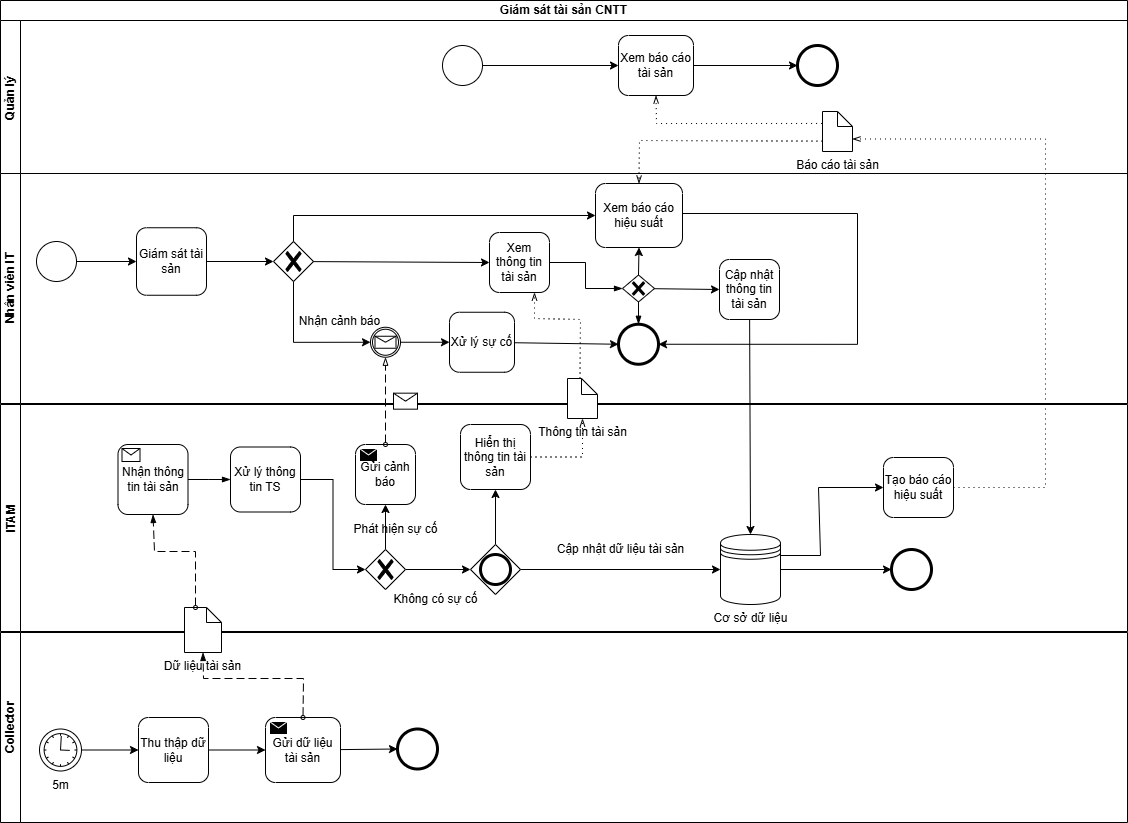
\includegraphics[width=\linewidth]{Images/C5/BPMN/RITAM-Giám sát Tài sản CNTT.drawio.png}
%     \vspace{0.5cm}
%     \caption{Mô hình hóa nghiệp vụ giám sát tài sản}
% \end{figure}
%      \begin{itemize}[label=--]
%         \item \textbf{Thu thập dữ liệu tài sản:} 
%         \begin{itemize}[label=\textbullet]
%             \item Cứ 5 phút, phần mềm Collector được cài đặt tại máy tính (bao gồm cả máy tính để bàn và máy tính xách tay) thu thập dữ liệu về cấu hình phần cứng, phần mềm, hiệu năng (RAM, CPU, bộ nhớ).
%             \item Dữ liệu mà Collector thu thập được sẽ gửi đến hệ thống quản lý tài sản - ITAM .
%         \end{itemize}
%         \item \textbf{Xử lý và quản lý dữ liệu tài sản CNTT:}
%         \begin{itemize}[label=\textbullet]
%             \item Hệ thống ITAM tiếp nhận dữ liệu tài sản CNTT theo thời gian thực từ Collector.
%             \item Hệ thống sẽ xử lý, phân tích và lưu trữ thông tin tài sản vào cơ sở dữ liệu. Vì sẽ có nhiều thông tin từ nhiều tài sản gửi lên cùng một lúc nên hệ thống sẽ sử dụng Kafka như trung gian để tổng hợp, phân phối dữ liệu.
%             \item Trong trường hợp không có sự cố, thì dữ liệu tài sản sẽ được cập nhật vào cơ sở dữ liệu, đồng thời sẽ được hiển thị ở màn hình nhân viên IT.
%         \end{itemize}
%         \item \textbf{Xử lý sự cố tài sản}
%         \begin{itemize}[label=\textbullet]
%             \item Qua quá trình xử lý dữ liệu từ tài sản, nếu phát hiện sự cố, hệ thống ITAM sẽ gửi cảnh báo đến Nhân viên IT. Sau đó Nhân viên IT bắt đầu quy trình xử lý sự cố.
%         \end{itemize}       
%         \item \textbf{Giám sát tài sản}
%         \begin{itemize}[label=\textbullet]
%             \item Trong quy trình giám sát tài sản, nhân viên IT có thể xem thông tin chi tiết tài sản, báo cáo hiệu suất, cập nhật thông tin tài sản, và xử lý sự cố khi có cảnh báo.
%             \item Quản lý cũng có thể xem các bảng tổng quan về tình trạng tài sản
%         \end{itemize}
        
%     \end{itemize}
% %----------%
%     \item \textbf{Quản lý vòng đời tài sản}\\
%     Vòng đời tài sản bao gồm các giai đoạn như sau: mua sắm, triển khai, sử dụng, thanh lý.
%      \begin{figure}[H]
%     \centering
%     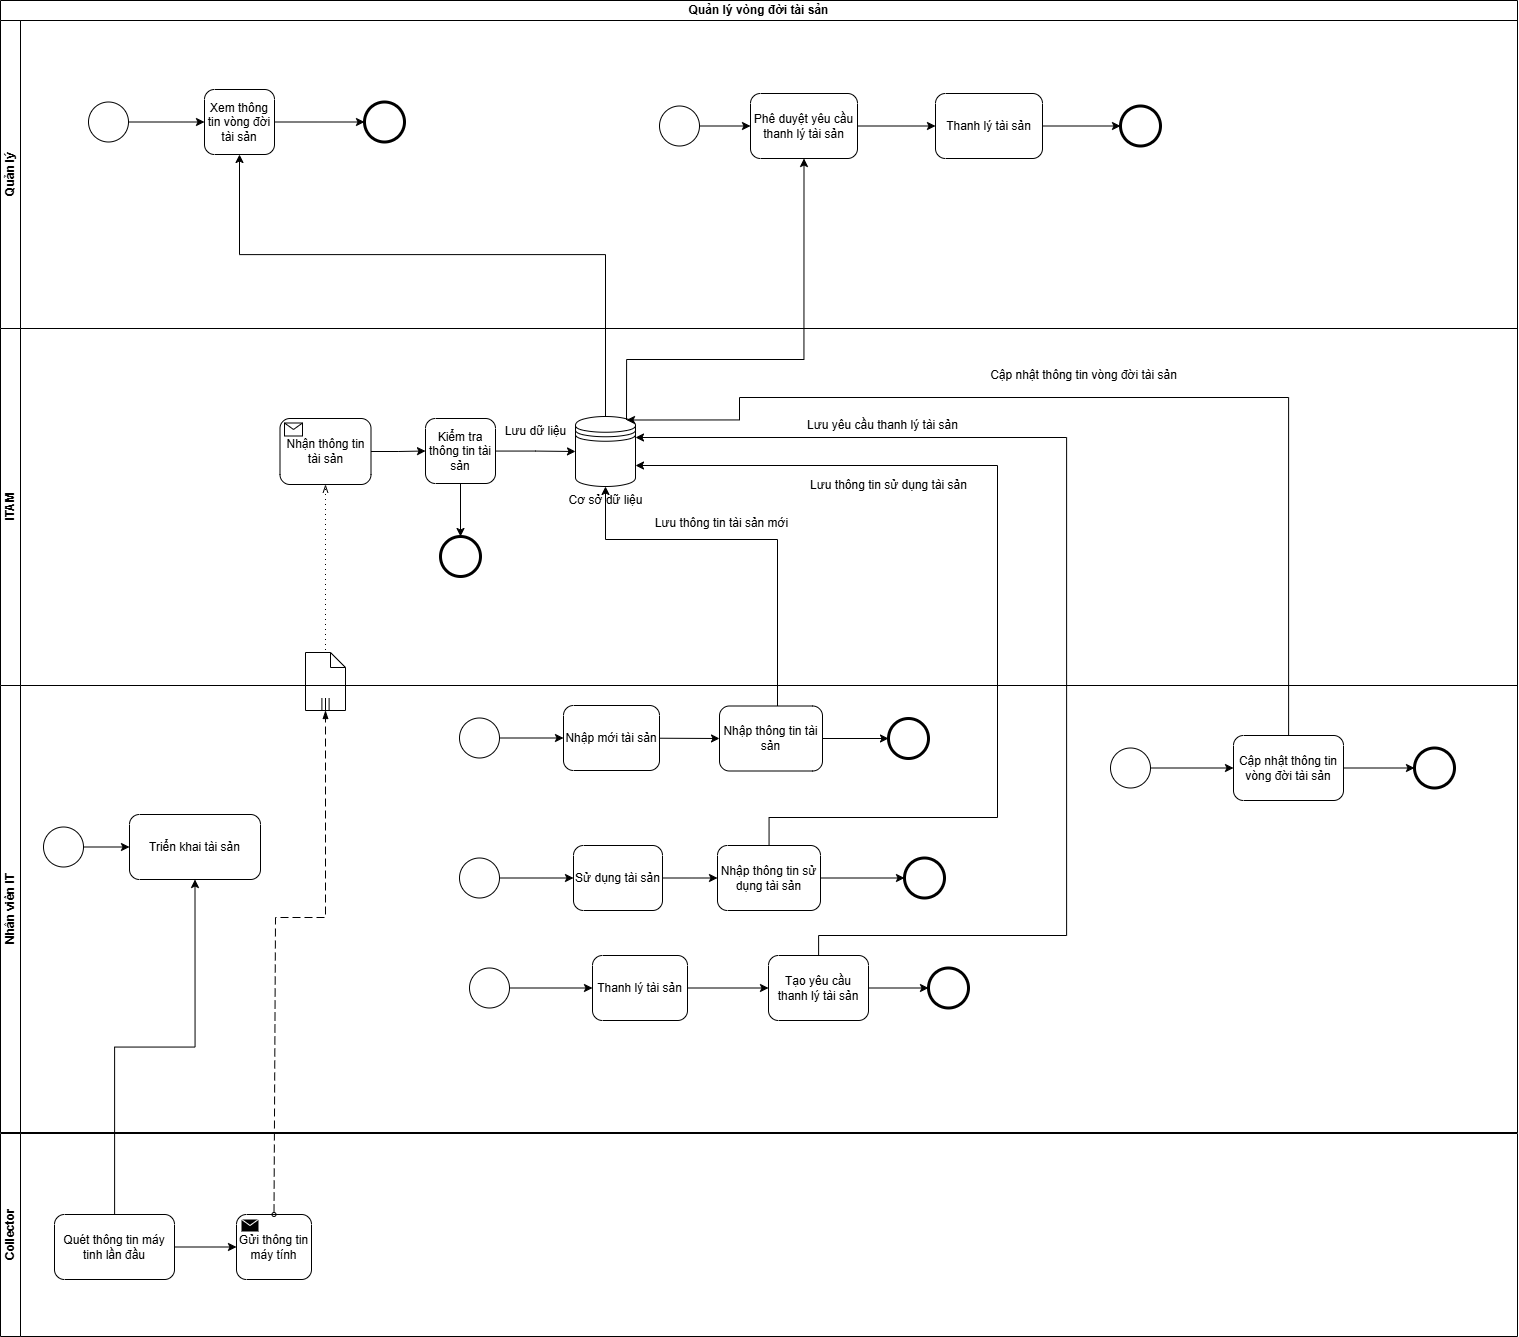
\includegraphics[width=\linewidth]{Images/C5/BPMN/RITAM-Quản lý vòng đời tài sản.drawio.png}
%     \vspace{15pt}
%     \caption{Mô hình hóa nghiệp vụ Quản lý vòng đời tài sản}
% \end{figure}
%     \begin{itemize}[label=--]
%        \item \textbf{Nhập mới tài sản:}
%        \begin{itemize}[label=\textbullet]
%            \item Sau khi hoàn tất giai đoạn mua sắm tài sản, Nhân viên IT nhận các thiết bị sẽ tiến hành nhập thông tin tài sản trên hệ thống.
%            \item Đối với các loại tài sản rời như Ổ cứng, Ram, card mạng, nhân viên có thể nhập trước các thông tin cơ bản. Tương tự đối với máy tính để bàn, máy tính Laptop, nhân viên IT nhập các thông tin cơ bản như hệ điều hành, mẫu mã, số seri.       
%        \end{itemize}
%        \item \textbf{Triển khai tài sản:}
%        \begin{itemize}[label=\textbullet]
%            \item Sau khi đã nhập xong thông tin, nhân viên IT tiến hành cài đặt tool và cấu hình lại để thu thập dữ liệu chi tiết phần cứng và phần mềm tại mỗi máy tính, rồi khởi động để bắt đầu quá trình thu thập dữ liệu lần đầu. 
%            \item Hệ thống tiếp nhận dữ liệu, kiểm tra dữ liệu và lưu dữ liệu chi tiết bao gồm dữ liệu về CPU, RAM, Ổ cứng, Card mạng, GPU (nếu có). 
%        \end{itemize}
%        \item \textbf{Sử dụng tài sản:}
%        \begin{itemize}[label=\textbullet]
%            \item Sau khi triển khai xong, nhân viên IT sẽ nhập thông tin sử dụng tài sản.
%            \item Hệ thống ghi nhận và cập nhật ở cơ sở dữ liệu.
%        \end{itemize}
%        \item \textbf{Thanh lý tài sản}:
%        \begin{itemize}[label=\textbullet]
%            \item Nhân viên tạo yêu cầu thanh lý tài sản.
%            \item Hệ thống ghi nhận và lưu lại cơ sở dữ liệu.
%            \item Quản lý sau đó có thể phê duyệt yêu cầu thanh lý tài sản. Hệ thống ghi nhận và lưu lại trạng thái đơn yêu cầu.
%            \item Sau khi đơn yêu cầu thanh lý đã được phê duyệt, nhân viên tiến hành thanh lý tài sản.
%        \end{itemize}
%     \end{itemize}
% %----------%
% %     \item Quản lý Dữ liệu Phần cứng và Phần mềm
% %      \begin{figure}[H]
% %     \centering
% %     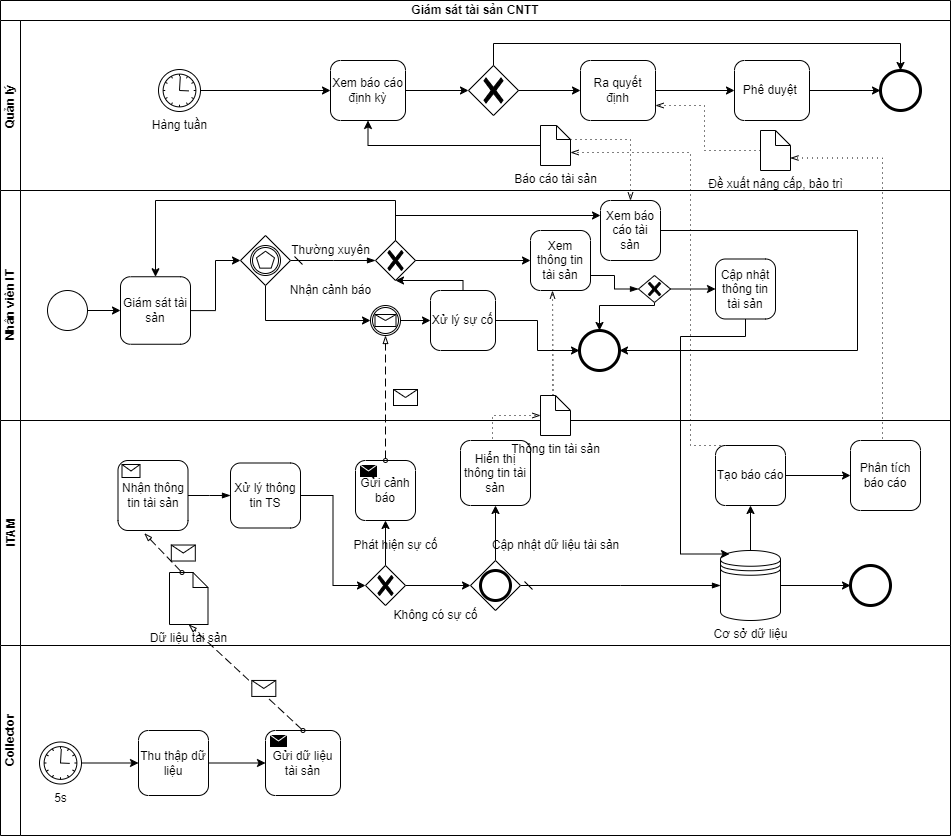
\includegraphics[width=\linewidth]{Images/C5/BPMN/BPMN-Giám sát Tài sản CNTT.png}
% %     \vspace{5pt}
% %     \caption{Mô hình hóa nghiệp vụ giám sát tài sản}
% % \end{figure}
%     \item \textbf{Cảnh báo}
%      \begin{figure}[H]
%     \centering
%     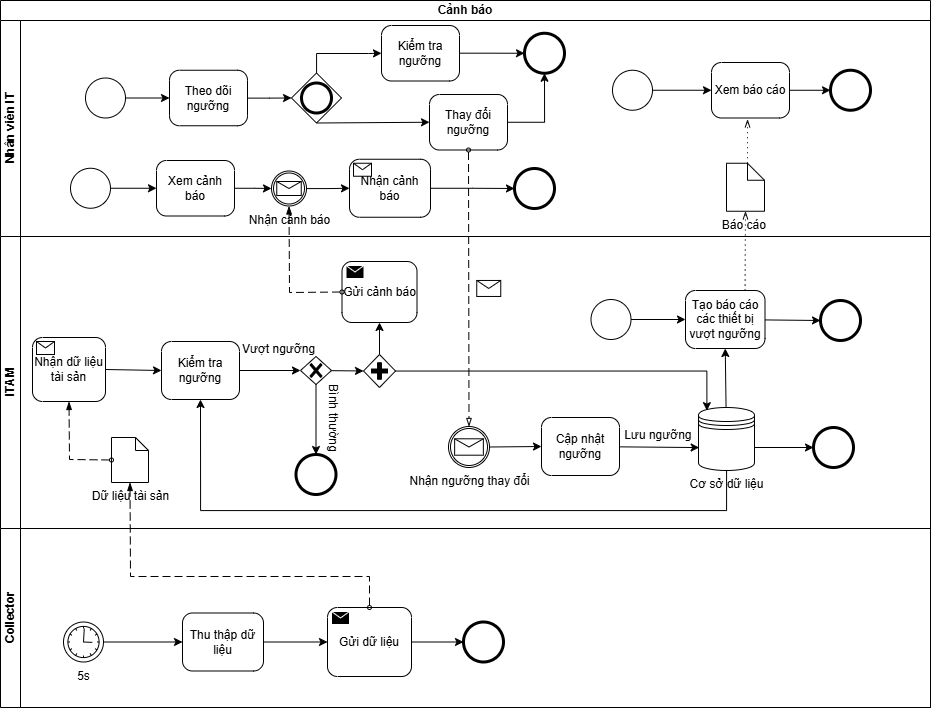
\includegraphics[width=\linewidth]{Images/C5/BPMN/BPMN-Cảnh báo.drawio.png}
%     \vspace{5pt}
%     \caption{Mô hình hóa nghiệp vụ Cảnh báo}
% \end{figure}
%     \begin{itemize}[label=--]
%         \item \textbf{Kiểm tra ngưỡng:}
%         \begin{itemize}[label=\textbullet]
%             \item Cứ 5 phút, Collector thu thập dữ liệu và gửi dữ liệu này đến hệ thống ITAM.
%             \item Hệ thống ITAM sau khi nhận dữ liệu sẽ kiểm tra thiết bị có vượt ngưỡng hay không. 
%             \item Nếu có tình trạng vượt ngưỡng, hệ thống sẽ gửi cảnh báo đến nhân viên IT phụ trách đồng thời lưu lại cảnh báo vào cơ sở dữ liệu. 
%             \item Nhân viên IT có thể xem các cảnh báo của các thiết bị vượt ngưỡng trên hệ thống.
%         \end{itemize}
%         \item \textbf{Theo dõi ngưỡng:}
%         \begin{itemize}[label=\textbullet]
%             \item Nhân viên IT có thể kiểm tra thông tin ngưỡng của các loại thiết bị.
%             \item Khi nhân viên thay đổi ngưỡng, hệ thống sẽ ghi nhận và thay đổi các chỉ số ở cơ sở dữ liệu.
%         \end{itemize}
%         \item \textbf{Báo cáo về các thiết bị vượt ngưỡng}
%         \begin{itemize}[label=\textbullet]
%             \item Khi nhân viên IT có nhu cầu xem báo cáo tổng quan về các thiết bị vượt ngưỡng, hệ thống sẽ tạo báo cáo từ cơ sở dữ liệu.
%         \end{itemize}
%     \end{itemize}
% %----------%
%     \item \textbf{Quản lý yêu cầu nâng cấp}
%     \begin{figure}[H]
%     \centering
%     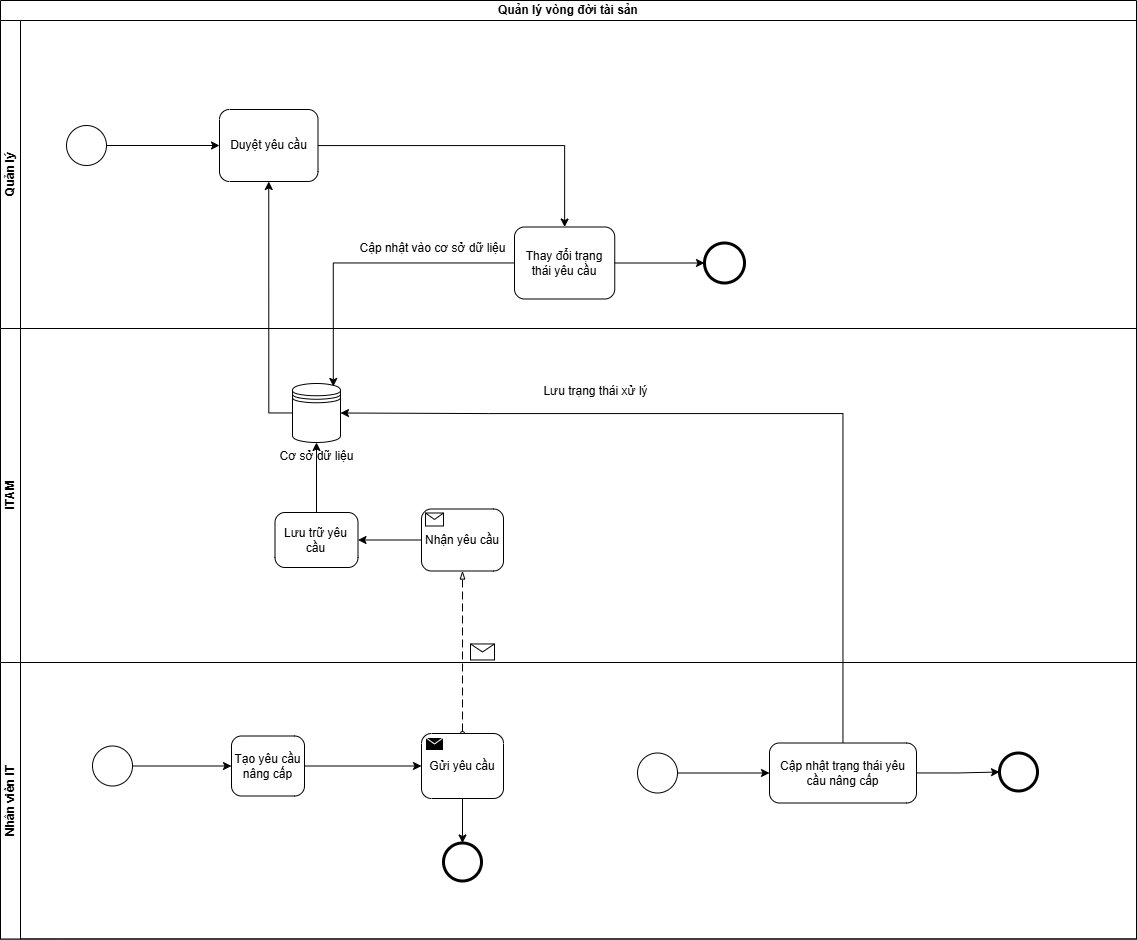
\includegraphics[width=0.8\linewidth]{Images/C5/BPMN/RITAM-Quản lý yêu cầu nâng cấp.drawio.png}
%     \vspace{10pt}
%     \caption{Mô hình hóa nghiệp vụ Quản lý yêu cầu nâng cấp tài sản}
% \end{figure}
%     \begin{itemize}[label=--]
%         \item Trong quá trình sử dụng tài sản, khi các thiết bị cũ cần được thay thế, nâng cấp, người dùng tài sản có thể báo cho nhân viên IT để tiến hành nâng cấp, thay thế tài sản.
%         \item Nhân viên khi nhận được yêu cầu từ người dùng tài sản sẽ tiến hành tạo yêu cầu nâng cấp tài sản.
%         \item Hệ thống sẽ lưu yêu cầu nâng cấp tài sản vào cơ sở dữ liệu và đợi phê duyệt từ quản lý.
%         \item Quản lý phê duyệt yêu cầu nâng cấp. Sau đó, hệ thống sẽ cập nhật trạng thái đã phê duyệt cho đơn yêu cầu nâng cấp.
%         \item Sau khi yêu cầu đã được phê duyệt thì nhân viên sẽ tiến hành nâng cấp hoặc thay thế tài sản. Khi hoàn thành nhân viên phải cập nhật trạng thái cho yêu cầu nâng cấp đã hoàn tất.
%         \item Khi hoàn tất yêu cầu nâng cấp, Tool sẽ tự động quét và gửi dữ liệu mới lên hệ thống. Hệ thống sau đó tiếp nhận và cập nhật thông tin vào cơ sở dữ liệu.
%     \end{itemize}
% %----------%    
%     \item \textbf{Quản lý sự cố và bảo trì}
%     \begin{figure}[H]
%     \centering
%     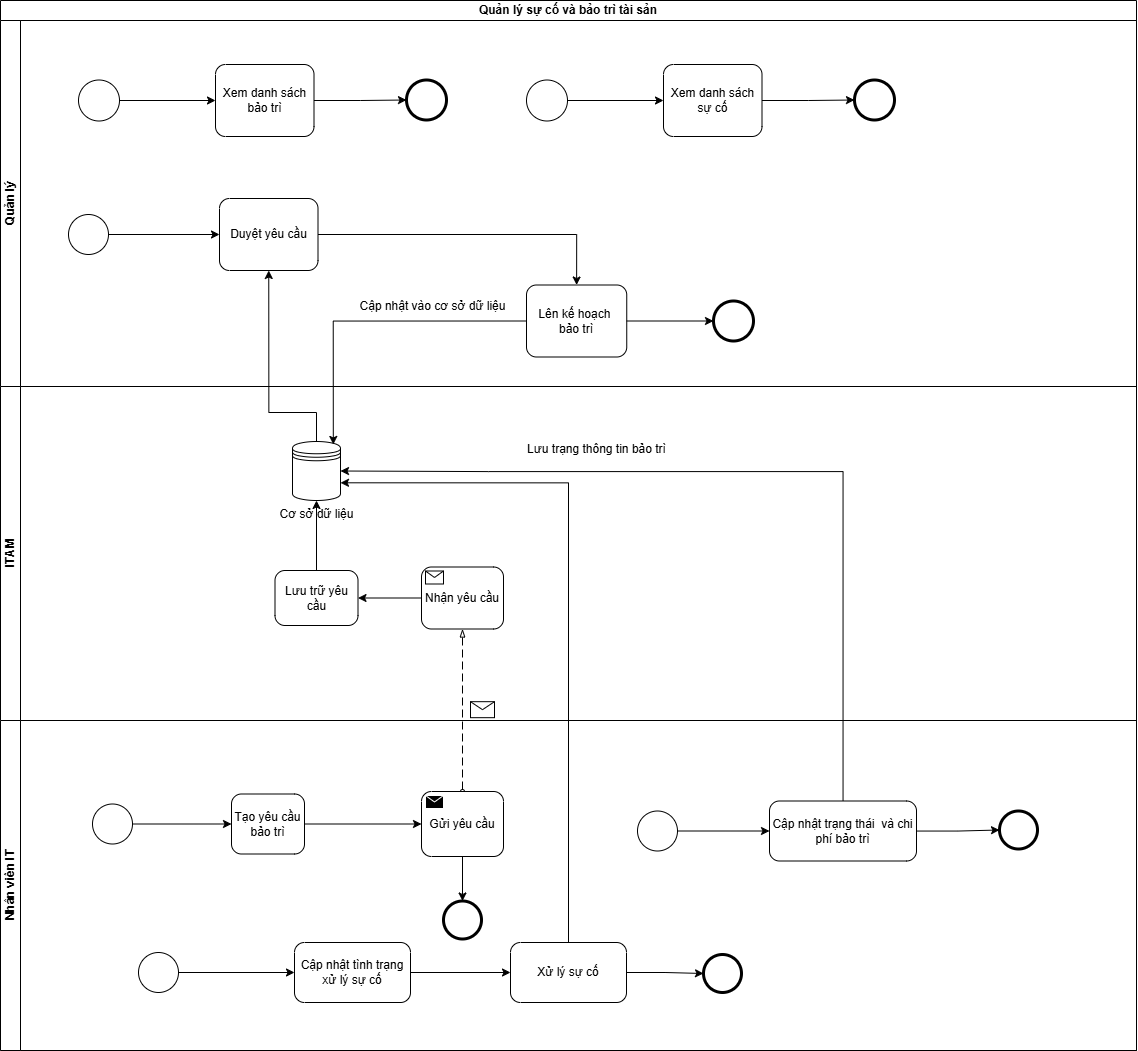
\includegraphics[width=0.8\linewidth]{Images/C5/BPMN/RITAM-Quản lý sự cố và bảo trì.drawio.png}
%     \vspace{10pt}
%     \caption{Mô hình hóa nghiệp vụ Quản lý sự cố và bảo trì tài sản}
% \end{figure}
%     \begin{itemize}[label=--]
%         \item \textbf{Quản lý sự cố tài sản}
%         \begin{itemize}[label=\textbullet]
%             \item Khi có sự cố tài sản, nhân viên IT sẽ lưu lại sự cố trên hệ thống và tiến hành xử lý sự cố.
%             \item Sau khi xử lý xong sự cố, nhân viên IT sẽ cập nhật trạng thái sự cố trên hệ thống.
%             \item Cả nhân viên IT và quản lý đều có thể xem lại lịch sử sự cố của từng máy.
%         \end{itemize}
%         \item \textbf{Quản lý bảo trì tài sản}
%         \begin{itemize}[label=\textbullet]
%             \item Nhân viên IT tạo yêu cầu bảo trì tài sản.
%             \item Hệ thống tiếp nhận và lưu yêu cầu bảo trì tài sản.
%             \item Quản lý phê duyệt yêu cầu bảo trì tài sản.
%             \item Nhân viên IT xác nhận thực hiện bảo trì, sau đó lên kế hoạch bảo trì tài sản.
%             \item Sau khi hoàn tất bảo trì tài sản, nhân viên IT cập nhật trạng thái và chi phí bảo trì.
%         \end{itemize}
%     \end{itemize}
% %----------%
%     \item \textbf{Quản lý Đơn đặt hàng}
%      \begin{figure}[H]
%     \centering
%     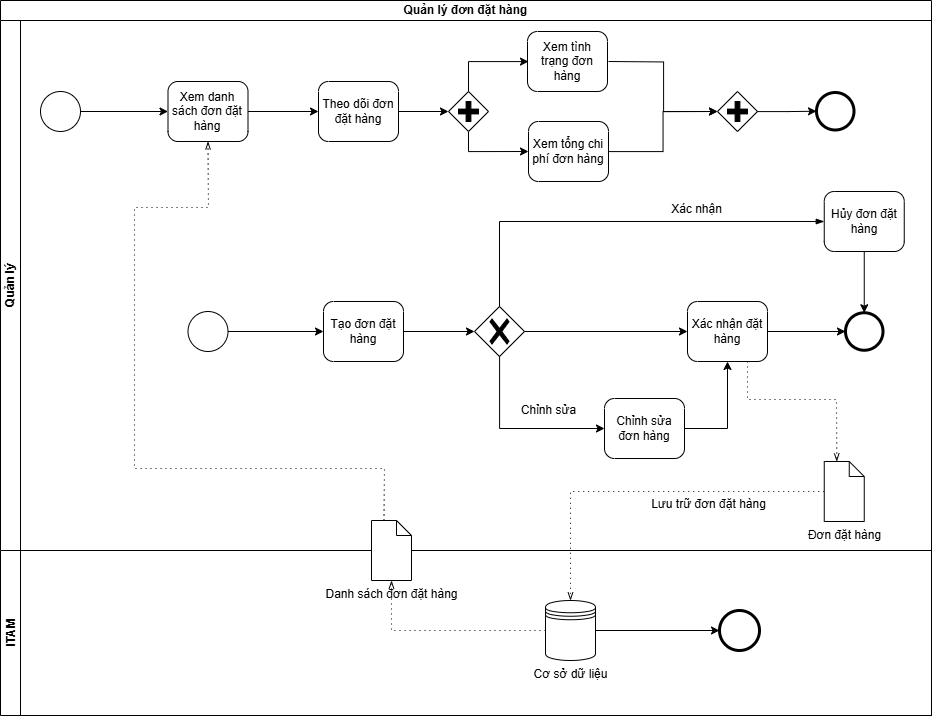
\includegraphics[width=\linewidth]{Images/C5/BPMN/RITAM-Quản lý đơn đặt hàng.drawio.png}
%     \vspace{5pt}
%     \caption{Mô hình hóa nghiệp vụ Quản lý đơn đặt hàng}
% \end{figure}
%     \begin{itemize}[label=--]
%         \item  \textbf{Tạo đơn đặt hàng:}
%         \begin{itemize}[label=\textbullet]
%             \item Quản lý tạo đơn đặt hàng trên hệ thống khi có nhu cầu mua sắm tài sản.
%             \item Sau khi tạo đơn hàng thì phải xác nhận đơn hàng, người tạo có thể chỉnh sửa rồi xác nhận lại đơn hàng. Quản lý phải gán mã nhân viên xử lý đơn hàng khi nhận hàng.
%             \item Đơn hàng sau khi xác nhận sẽ được lưu trữ vào cơ sở dữ liệu. 
%             \item Ngoài ra Quản lý có thể hủy đơn đặt hàng nếu trong quá trình tạo đơn có sai sót.
%         \end{itemize}
%         \item \textbf{Xem danh sách các đơn hàng:}
%         \begin{itemize}[label=\textbullet]
%             \item Quản lý có thể xem danh sách các đơn đặt hàng, họ có thể xem cụ thể một đơn hàng
%             \item Đơn hàng bao gồm các thông tin cơ bản, tình trạng và tổng chi phí cho đơn hàng ,thông tin nhân viên xử lý đơn hàng đó.
%         \end{itemize}
%     \end{itemize}
% %----------%
% \end{enumerate}

% \subsubsection{ Mô hình hóa tương tác}
% \begin{itemize}[label=--]
% \item{Use case toàn hệ thống}
% \begin{figure}[H]
%     \centering
%     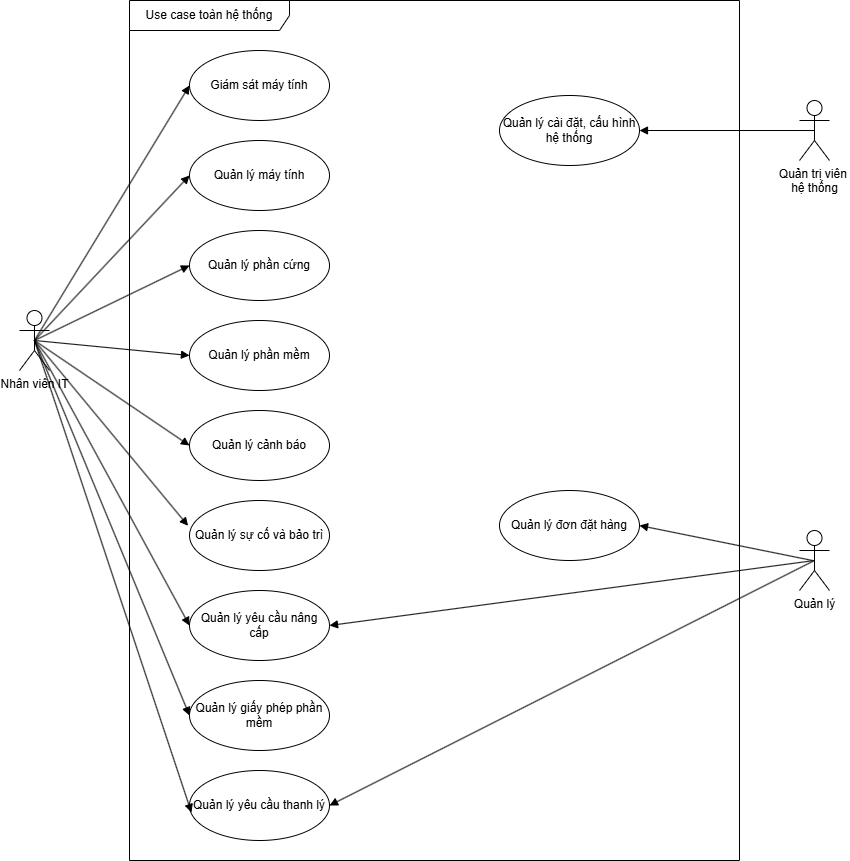
\includegraphics[width=\linewidth]{Images/C5/UseCaseDiagrams/Use-case-General.drawio.png}
%     \vspace{5pt}
%     \caption{Use case toàn hệ thống}
% \end{figure}

% % \subsubsubsection{ Use case Đăng nhập}
% % \begin{figure}[H]
% %     \centering
% %     \includegraphics[width=\linewidth]{Images/C5/UseCaseDiagrams/Use-case-Dang-nhap.drawio.png}
% %     \vspace{5pt}
% %     \caption{Use case Đăng nhập}
% % \end{figure}
% %%----------------------------------
% % \begin{table}[H]
% %         \centering
% %         \begin{tabular}{|p{4cm}|p{10cm}|}
% %             \hline
% %             Tên use-case & Đăng nhập\\
% %             \hline
% %             Đối tượng & Nhân viên IT, Quản lý, Quản trị viên hệ thống \\
% %             \hline
% %             Mô tả & Nhân viên IT, Quản lý, Quản trị viên hệ thống thực hiện đăng nhập vào hệ thống ITAM \\
% %             \hline
% %             Diều kiện kích hoạt &  Nhân viên IT, Quản lý, Quản trị viên hệ thống bấm vào mục "Đăng nhập"\\
% %             \hline
% %             Tiền điều kiện & Nhân viên IT, Quản lý, Quản trị viên hệ thống chưa đăng nhập vào hệ thống, đã có tài khoản và mật khẩu \\
% %             \hline
% %             Hậu điều kiện & Nhân viên IT, Quản lý, Quản trị viên hệ thống đăng nhập vào hệ thống thành công \\
% %             \hline
% %             Luồng tương tác chính & 
% %             \begin{enumerate}
% %                 \item Nhân viên IT, Quản lý, Quản trị viên hệ thống truy cập vào màn hình đăng nhập.
% %                 \item Nhân viên IT, Quản lý, Quản trị viên hệ thống điền thông tin tài khoản và mật khẩu.
% %                 \item Nếu thông tin đăng nhập đúng và chính xác, Nhân viên IT, Quản lý, Quản trị viên hệ thống đăng nhập vào hệ thống và chuyển đến trang chủ.
% %             \end{enumerate}\\
% %             \hline
% %             % Luồng tương tác thay thế& b \\
% %             % \hline
% %             Luồng tương tác ngoại lệ & Nếu trong quá trình xác thực tài khoản có vấn đề hay lỗi thì hệ thống sẽ trả về lỗi tài khoản chưa được xác thực thành công. Nếu tài khoản không tồn tại hệ thống trả về lỗi không tồn tại tài khoản. Nếu sai mật khẩu hệ thống trả về lỗi sai mật khẩu \\
% %             \hline
% %         \end{tabular}
% %         \caption{Đặc tả Use case Đăng nhập}
% %         \label{tab:my_label}
% % oi\end{table}

% \item{ Use case Giám sát máy tính}
% \begin{figure}[H]
%     \centering
%     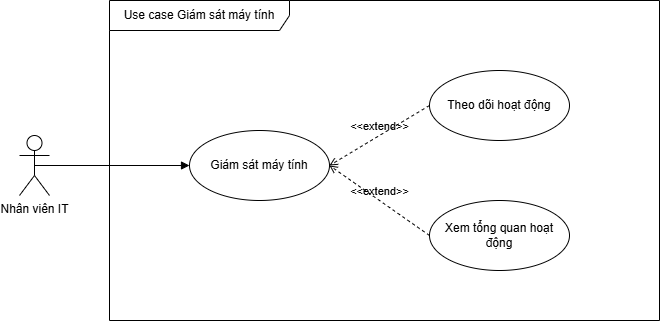
\includegraphics[width=\linewidth]{Images/C5/UseCaseDiagrams/Use-case-Giam-sat-may-tinh.drawio.png}
%     \vspace{5pt}
%     \caption{Use case Giám sát máy tính}
% \end{figure}

% \begin{table}[H]
%     \centering
%     \caption{Đặc tả Use case Giám sát máy tính}
%     \begin{tabular}{|p{4cm}|p{10cm}|}
%         \hline
%         Tên use-case & Giám sát máy tính\\
%         \hline
%         Đối tượng & Nhân viên IT \\
%         \hline
%         Mô tả & Nhân viên IT có thể giám sát hoạt động của máy tính, bao gồm theo dõi hoạt động và xem tổng quan hoạt động. \\
%         \hline
%         Điều kiện kích hoạt & Nhân viên IT chọn vào mục "Giám sát máy tính" trên giao diện hệ thống.\\
%         \hline
%         Tiền điều kiện & 
%         \begin{itemize}
%             \item Nhân viên IT đã đăng nhập vào hệ thống.
%             \item Nhân viên IT có quyền truy cập tính năng giám sát máy tính.
%         \end{itemize}\\
%         \hline
%         Hậu điều kiện & Nhân viên IT giám sát thành công các hoạt động của máy tính. \\
%         \hline
%         Luồng tương tác chính &
%         \begin{enumerate}
%             \item Nhân viên IT truy cập vào mục "Giám sát máy tính".
%             \item Nhân viên IT chọn "Hoạt động" để xem giao diện giám sát máy tính.
%             \item Hệ thống hiển thị giao diện giám sát máy tính theo thời gian thực.
%         \end{enumerate}\\
%         \hline
%         Luồng tương tác thay thế&
%         Tại bước 2:
%         \newline
%             2.1. Nhân viên IT chọn "Tổng quan hoạt động" để xem tổng quan hoạt động của các máy tính trong hệ thống.
%         \newline 
%             2.2. Hệ thống hiển thị giao diện tổng quan hoạt động của các máy tính trong hệ thống.
%         \\
%         \hline
%         Luồng tương tác ngoại lệ & 
%         Tại bước 3: Hệ thống lỗi khi hiển thị giao diện giám sát theo thời gian thực, hệ thống báo lỗi.
%         \newline
%         Tại bước 2.2: Hệ thống lỗi khi hiển thị tổng quan hoạt động của các máy tính, hệ thống báo lỗi.
%         \\
%         \hline
%     \end{tabular}
    
%     \label{tab:use_case_monitor}
% \end{table}


% \item{ Use case Quản lý máy tính}
% \begin{figure}[H]
%     \centering
%     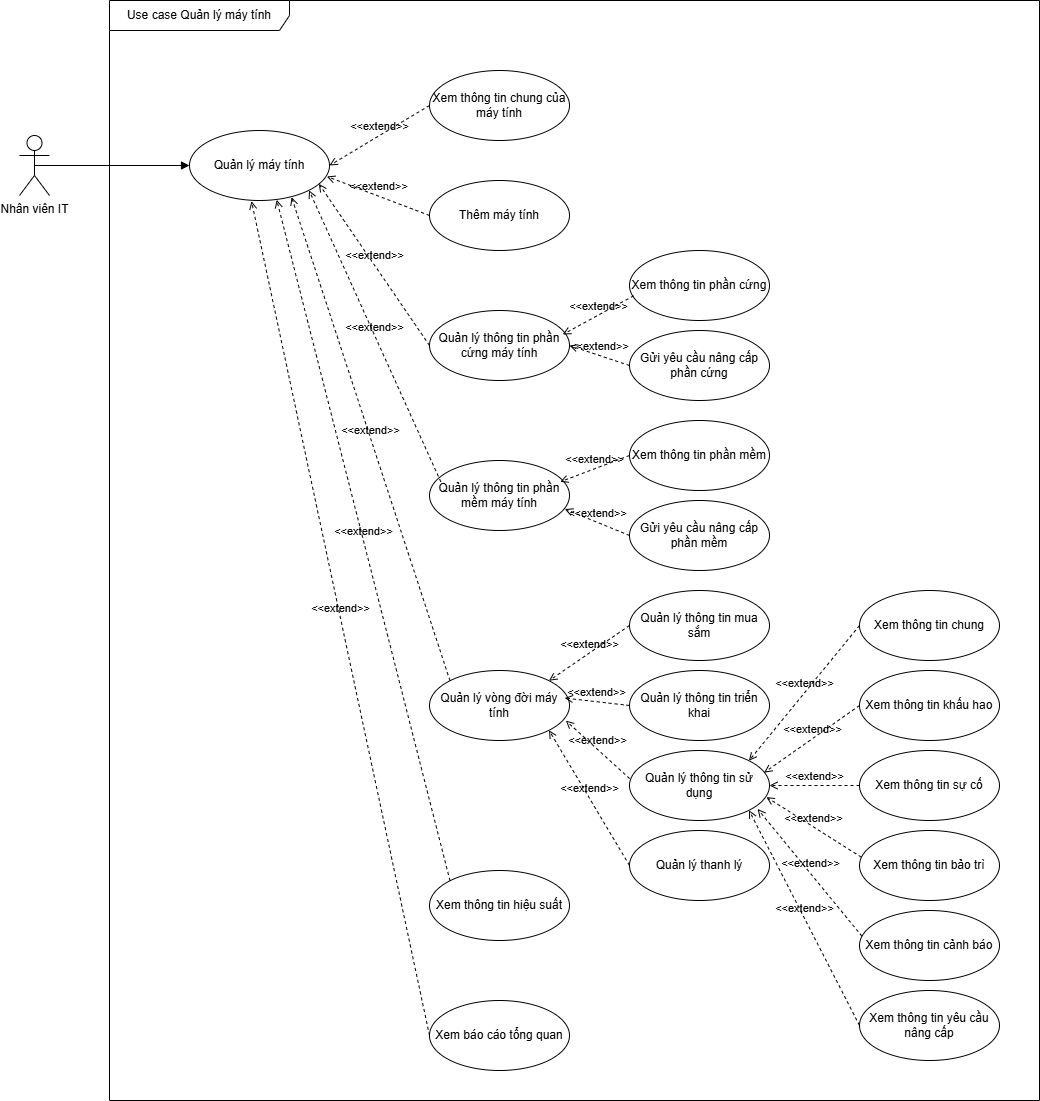
\includegraphics[width=\linewidth]{Images/C5/UseCaseDiagrams/Use-case-Quan-ly-may-tinh.drawio.png}
%     \vspace{5pt}
%     \caption{Use case Quản lý máy tính}
% \end{figure}

% \begin{table}[H]
%         \centering
%         \caption{Đặc tả Use case Xem thông tin chung của máy tính}
%         \begin{tabular}{|p{4cm}|p{10cm}|}
%             \hline
%             Tên use-case & Xem thông tin chung của máy tính\\
%             \hline
%             Đối tượng & Nhân viên IT \\
%             \hline
%             Mô tả & Nhân viên IT có thể thực hiện xem thông tin chung của máy tính \\
%             \hline
%             Diều kiện kích hoạt & Nhân viên IT chọn máy tính cần xem thông tin \\
%             \hline
%             Tiền điều kiện & Nhân viên IT đã đăng nhập vào hệ thống, có quyền truy cập vào tính năng Quản lý máy tính. \\
%             \hline
%             Hậu điều kiện & Nhân viên IT có thể thực hiện xem thông tin chung của máy tính thành công \\
%             \hline
%             Luồng tương tác chính &
%             \begin{enumerate}
%                 \item Nhân viên IT chọn "Quản lý máy tính" ở giao diện chính của hệ thống.
%                 \item Hệ thống hiển thị danh sách các máy tính.
%                 \item Nhân viên IT chọn máy tính cần xem thông tin từ danh sách.
%                 \item Hệ thống hiện thị thông tin về máy tính đã chọn.
%             \end{enumerate}\\
%             \hline
%             Luồng tương tác thay thế&  
%             Không có\\
%             \hline
%             Luồng tương tác ngoại lệ & 
%             Tại bước 2: Hệ thống lỗi trong việc hiển thị danh sách các máy tính, hệ thống báo lỗi.
            
%             Tại bước 4: Hệ thống lỗi trong việc hiển thị thông tin máy tính, hệ thống báo lỗi.
%             \\
%             \hline
%         \end{tabular}
        
%         \label{tab:my_label}
% \end{table}

% \begin{table}[H]
%         \centering
%         \caption{Đặc tả Use case Thêm máy tính}
%         \begin{tabular}{|p{4cm}|p{10cm}|}
%             \hline
%             Tên use-case & Thêm máy tính\\
%             \hline
%             Đối tượng & Nhân viên IT \\
%             \hline
%             Mô tả & Nhân viên IT có thể thực hiện thêm máy tính \\
%             \hline
%             Diều kiện kích hoạt & Nhân viên IT chọn "Thêm máy tính" \\
%             \hline
%             Tiền điều kiện & Nhân viên IT đã đăng nhập vào hệ thống, có quyền truy cập vào tính năng Quản lý máy tính. \\
%             \hline
%             Hậu điều kiện & Nhân viên IT có thể thực hiện thêm máy tính thành công \\
%             \hline
%             Luồng tương tác chính &
%             \begin{enumerate}
%                 \item Nhân viên IT chọn "Quản lý máy tính" ở giao diện chính của hệ thống.
%                 \item Hệ thống hiển thị danh sách các máy tính và nút "Thêm máy tính"
%                 \item Nhân viên IT chọn nút "Thêm máy tính".
%                 \item Hệ thống hiện thị trang biểu mẫu thêm máy tính.
%                 \item Nhân viên IT thực hiện điền thông tin máy tính cần thêm mới và nhấn nút "Lưu".
%                 \item Hệ thống kiểm tra và ghi nhận thông tin máy tính mới và báo thành công.
%             \end{enumerate}\\
%             \hline
%             Luồng tương tác thay thế&  
%             Tại bước 5: Nếu muốn hủy bỏ thêm máy tính, Nhân viên IT bấm "Trở về". Tiếp tục bước 2\\
%             \hline
%             Luồng tương tác ngoại lệ & 
%             Tại bước 2: Hệ thống lỗi trong việc hiển thị danh sách các máy tính, hệ thống báo lỗi.
            
%             Tại bước 4: Hệ thống lỗi trong việc kiểm tra và ghi nhận thông tin máy tính mới, hệ thống báo lỗi.

%             Tại bước 4: Hệ thống kiểm tra thông tin máy tính mới và không cho phép lưu, hệ thống báo lỗi cho người dùng.
%             \\
%             \hline
%         \end{tabular}
        
%         \label{tab:my_label}
% \end{table}

% \begin{table}[H]
%         \centering
%         \caption{Đặc tả Use case Quản lý thông tin phần cứng máy tính}
%         \begin{tabular}{|p{4cm}|p{10cm}|}
%             \hline
%             Tên use-case & Quản lý thông tin phần cứng máy tính\\
%             \hline
%             Đối tượng & Nhân viên IT \\
%             \hline
%             Mô tả & Nhân viên IT có thể thực hiện quản lý thông tin phần cứng máy tính \\
%             \hline
%             Diều kiện kích hoạt & Nhân viên IT chọn "Thông tin phần cứng" \\
%             \hline
%             Tiền điều kiện & Nhân viên IT đã đăng nhập vào hệ thống, có quyền truy cập vào tính năng Quản lý máy tính. \\
%             \hline
%             Hậu điều kiện & Nhân viên IT có thể thực hiện quản lý thông tin phần cứng máy tính thành công \\
%             \hline
%             Luồng tương tác chính &
%             \begin{enumerate}
%                 \item Nhân viên IT chọn "Quản lý máy tính" ở giao diện chính của hệ thống.
%                 \item Hệ thống hiển thị danh sách các máy tính.
%                 \item Nhân viên IT chọn máy tính cần quản lý.
%                 \item Hệ thống hiện thị thông tin chi tiết của máy tính.
%                 \item Nhân viên IT chọn nút "Thông tin phần cứng"
%                 \item Hệ thống hiển thị thông tin về phần cứng máy tính và nút "Gửi yêu cầu nâng cấp".
%                 \item Nhân viên IT chọn nút "Gửi yêu cầu nâng cấp".
%                 \item Hệ thống xuất hiện biểu mẫu "Yêu cầu nâng cấp".
%                 \item Nhân viên IT điền vào biểu mẫu và nhấn nút "Gửi".
%                 \item Hệ thống kiểm tra và lưu yêu cầu nâng cấp.
%             \end{enumerate}\\
%             \hline
%             Luồng tương tác thay thế&  
%             Tại bước 6: Nhân viên IT bấm "Trở về". Tiếp tục bước 2

%             Tại bước 9: Nếu muốn hủy bỏ yêu cầu nâng cấp phần cứng, bấm "Hủy".
%             \\
%             \hline
%             Luồng tương tác ngoại lệ & 
%             Tại bước 2: Hệ thống lỗi trong việc hiển thị danh sách các máy tính, hệ thống báo lỗi.

%             Tại bước 6: Hệ thống lỗi trong việc hiển thị thông tin phần cứng, hệ thống báo lỗi.
            
%             Tại bước 10: Hệ thống lỗi trong việc kiểm tra và ghi nhận yêu cầu nâng cấp, hệ thống báo lỗi.

%             Tại bước 10: Hệ thống kiểm tra yêu cầu nâng cấp và không cho phép lưu, hệ thống báo lỗi cho người dùng.
%             \\
%             \hline
%         \end{tabular}
        
%         \label{tab:my_label}
% \end{table}

% \begin{table}[H]
%         \centering\
%         \caption{Đặc tả Use case Quản lý thông tin phần mềm máy tính}
%         \begin{tabular}{|p{4cm}|p{10cm}|}
%             \hline
%             Tên use-case & Quản lý thông tin phần mềm máy tính\\
%             \hline
%             Đối tượng & Nhân viên IT \\
%             \hline
%             Mô tả & Nhân viên IT có thể thực hiện quản lý thông tin phần mềm máy tính \\
%             \hline
%             Diều kiện kích hoạt & Nhân viên IT chọn "Thông tin phần mềm" \\
%             \hline
%             Tiền điều kiện & Nhân viên IT đã đăng nhập vào hệ thống, có quyền truy cập vào tính năng Quản lý máy tính. \\
%             \hline
%             Hậu điều kiện & Nhân viên IT có thể thực hiện quản lý thông tin phần mềm máy tính thành công \\
%             \hline
%             Luồng tương tác chính &
%             \begin{enumerate}
%                 \item Nhân viên IT chọn "Quản lý máy tính" ở giao diện chính của hệ thống.
%                 \item Hệ thống hiển thị danh sách các máy tính.
%                 \item Nhân viên IT chọn máy tính cần quản lý.
%                 \item Hệ thống hiện thị thông tin chi tiết của máy tính.
%                 \item Nhân viên IT chọn nút "Thông tin phần mềm"
%                 \item Hệ thống hiển thị danh sách thông tin về phần mềm máy tính và nút "Gửi yêu cầu nâng cấp".
%                 \item Nhân viên IT chọn nút "Gửi yêu cầu nâng cấp".
%                 \item Hệ thống xuất hiện biểu mẫu "Yêu cầu nâng cấp".
%                 \item Nhân viên IT điền vào biểu mẫu và nhấn nút "Gửi".
%                 \item Hệ thống kiểm tra và lưu yêu cầu nâng cấp.
%             \end{enumerate}\\
%             \hline
%             Luồng tương tác thay thế&  
%             Tại bước 6: Nhân viên IT bấm "Trở về". Tiếp tục bước 2

%             Tại bước 9: Nếu muốn hủy bỏ yêu cầu nâng cấp phần mềm, bấm "Hủy".
%             \\
%             \hline
%             Luồng tương tác ngoại lệ & 
%             Tại bước 2: Hệ thống lỗi trong việc hiển thị danh sách các máy tính, hệ thống báo lỗi.

%             Tại bước 6: Hệ thống lỗi trong việc hiển thị danh sách thông tin phần mềm, hệ thống báo lỗi.
            
%             Tại bước 10: Hệ thống lỗi trong việc kiểm tra và ghi nhận yêu cầu nâng cấp, hệ thống báo lỗi.

%             Tại bước 10: Hệ thống kiểm tra yêu cầu nâng cấp và không cho phép lưu, hệ thống báo lỗi cho người dùng.
%             \\
%             \hline
%         \end{tabular}
        
%         \label{tab:my_label}
% \end{table}

% \begin{table}[H]
%         \centering
%         \caption{Đặc tả Use case Quản lý vòng đời máy tính}
%         \begin{tabular}{|p{4cm}|p{10cm}|}
%             \hline
%             Tên use-case & Quản lý vòng đời máy tính\\
%             \hline
%             Đối tượng & Nhân viên IT \\
%             \hline
%             Mô tả & Nhân viên IT có thể thực hiện quản lý vòng đời máy tính \\
%             \hline
%             Diều kiện kích hoạt & Nhân viên IT chọn "Vòng đời tài sản" \\
%             \hline
%             Tiền điều kiện & Nhân viên IT đã đăng nhập vào hệ thống, có quyền truy cập vào tính năng Quản lý máy tính. \\
%             \hline
%             Hậu điều kiện & Nhân viên IT có thể thực hiện quản lý vòng đời máy tính thành công \\
%             \hline
%             Luồng tương tác chính &
%             \begin{enumerate}
%                 \item Nhân viên IT chọn "Quản lý máy tính" ở giao diện chính của hệ thống.
%                 \item Hệ thống hiển thị danh sách các máy tính.
%                 \item Nhân viên IT chọn máy tính cần quản lý.
%                 \item Hệ thống hiện thị thông tin chi tiết của máy tính.
%                 \item Nhân viên IT chọn nút "Vòng đời tài sản"
%                 \item Nhân viên IT chọn nút "Mua sắm"
%                 \item Hệ thống hiển thị thông tin về mua sắm tài sản.
%             \end{enumerate}\\
%             \hline
%             Luồng tương tác thay thế&  
%             Tại bước 6:
            
%             6.1.1. Nhân viên IT chọn "Triển khai".
            
%             6.1.2. Hệ thống hiển thị thông tin về triển khai máy tính.
            

%             Tại bước 6:
            
%             6.2.1. Nhân viên IT chọn "Sử dụng".
            
%             6.2.2. Hệ thống hiển thị thông tin về sử dụng máy tính bao gồm thông tin chung về sử dụng, thông tin khấu hao, thông tin về sự cố máy tính, thông tin về bảo trì, thông tin về cảnh báo, thông tin về yêu cầu nâng cấp của máy tính.


%             Tại bước 6:
            
%             6.3.1. Nhân viên IT chọn "Thanh lý".
            
%             6.3.2. Hệ thống hiển thị thông tin về thanh lý máy tính.

%             \\
%             \hline
%             Luồng tương tác ngoại lệ & 
%             Tại bước 2: Hệ thống lỗi trong việc hiển thị danh sách các máy tính, hệ thống báo lỗi.

%             Tại bước 7, 6.1.2, 6.2.2, 6.3.2: Hệ thống lỗi trong việc hiển thị thông tin, hệ thống báo lỗi.
%             \\
%             \hline
%         \end{tabular}
        
%         \label{tab:my_label}
% \end{table}

% \begin{table}[H]
%         \centering
%         \caption{Đặc tả Use case Xem thông tin hiệu suất}
%         \begin{tabular}{|p{4cm}|p{10cm}|}
%             \hline
%             Tên use-case & Xem thông tin hiệu suất\\
%             \hline
%             Đối tượng & Nhân viên IT \\
%             \hline
%             Mô tả & Nhân viên IT có thể thực hiện xem thông tin hiệu suất máy tính \\
%             \hline
%             Diều kiện kích hoạt & Nhân viên IT chọn "Hiệu suất máy tính" \\
%             \hline
%             Tiền điều kiện & Nhân viên IT đã đăng nhập vào hệ thống, có quyền truy cập vào tính năng Quản lý máy tính. \\
%             \hline
%             Hậu điều kiện & Nhân viên IT có thể thực hiện xem thông tin hiệu suất thành công \\
%             \hline
%             Luồng tương tác chính &
%             \begin{enumerate}
%                 \item Nhân viên IT chọn "Quản lý máy tính" ở giao diện chính của hệ thống.
%                 \item Hệ thống hiển thị danh sách các máy tính.
%                 \item Nhân viên IT chọn máy tính cần quản lý.
%                 \item Hệ thống hiện thị thông tin chi tiết của máy tính.
%                 \item Nhân viên IT chọn nút "Hiệu suất máy tính"
%                 \item Hệ thống hiển thị thông tin về hiệu suất máy tính.
%             \end{enumerate}\\
%             \hline
%             Luồng tương tác thay thế&  
%             Tại bước 6: Nhân viên IT bấm "Trở về". Tiếp tục bước 2
%             \\
%             \hline
%             Luồng tương tác ngoại lệ & 
%             Tại bước 2: Hệ thống lỗi trong việc hiển thị danh sách các máy tính, hệ thống báo lỗi.

%             Tại bước 6: Hệ thống lỗi trong việc hiển thị hiệu suất, hệ thống báo lỗi.
%             \\
%             \hline
%         \end{tabular}
        
%         \label{tab:my_label}
% \end{table}

% \begin{table}[H]
%         \centering
%         \caption{Đặc tả Use case Xem báo cáo tổng quan}
%         \begin{tabular}{|p{4cm}|p{10cm}|}
%             \hline
%             Tên use-case & Xem báo cáo tổng quan\\
%             \hline
%             Đối tượng & Nhân viên IT \\
%             \hline
%             Mô tả & Nhân viên IT có thể thực hiện xem báo cáo tổng quan của các máy tính \\
%             \hline
%             Diều kiện kích hoạt & Nhân viên IT chọn "Báo cáo tổng quan" \\
%             \hline
%             Tiền điều kiện & Nhân viên IT đã đăng nhập vào hệ thống, có quyền truy cập vào tính năng Quản lý máy tính. \\
%             \hline
%             Hậu điều kiện & Nhân viên IT có thể thực hiện xem báo cáo tổng quan các máy tính thành công \\
%             \hline
%             Luồng tương tác chính &
%             \begin{enumerate}
%                 \item Nhân viên IT chọn "Quản lý máy tính" ở giao diện chính của hệ thống.
%                 \item Hệ thống hiển thị danh sách các máy tính.
%                 \item Nhân viên IT chọn "Báo cáo tổng quan".
%                 \item Hệ thống hiện thị báo cáo tổng quan về các máy tính.
%             \end{enumerate}\\
%             \hline
%             Luồng tương tác thay thế&  
%             Không có\\
%             \hline
%             Luồng tương tác ngoại lệ & 
%             Tại bước 2: Hệ thống lỗi trong việc hiển thị danh sách các máy tính, hệ thống báo lỗi.
            
%             Tại bước 4: Hệ thống lỗi trong việc hiển thị báo cáo tổng quan các máy tính, hệ thống báo lỗi.
%             \\
%             \hline
%         \end{tabular}
        
%         \label{tab:my_label}
% \end{table}

% \item{ Use case Quản lý phần cứng}
% \begin{figure}[H]
%     \centering
%     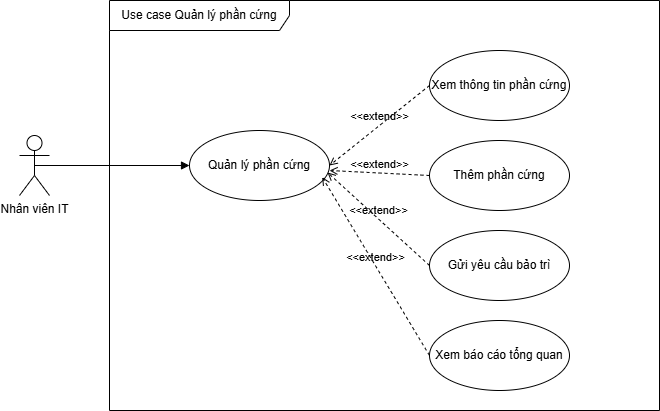
\includegraphics[width=\linewidth]{Images/C5/UseCaseDiagrams/Use-case-Quan-ly-phan-cung.drawio.png}
%     \vspace{5pt}
%     \caption{Use case Quản lý phần cứng}
% \end{figure}
% \begin{table}[H]
%         \centering
%         \caption{Đặc tả Use case Quản lý phần cứng}
%         \begin{tabular}{|p{4cm}|p{10cm}|}
%             \hline
%             Tên use-case & Quản lý phần cứng\\
%             \hline
%             Đối tượng & Nhân viên IT \\
%             \hline
%             Mô tả & Nhân viên IT thực hiện quản lý phần cứng \\
%             \hline
%             Diều kiện kích hoạt & Nhân viên IT bấm nút "Phần cứng" trên giao diện chính của hệ thống \\
%             \hline
%             Tiền điều kiện & Nhân viên IT đã đăng nhập vào hệ thống, có quyền truy cập vào tính năng Quản lý phần cứng. \\
%             \hline
%             Hậu điều kiện & Nhân viên IT thực hiện quản lý phần cứng thành công. \\
%             \hline
%             Luồng tương tác chính & 
%             \begin{enumerate}
%                 \item Nhân viên IT chọn "Phần cứng" ở giao diện chính của hệ thống.
%                 \item Hệ thống hiển thị danh sách các phần cứng.
%                 \item Nhân viên IT chọn phần cứng cần xem chi tiết.
%                 \item Hệ thống hiển thị thông tin chi tiết của phần cứng.
%             \end{enumerate}
%             \\
%             \hline
%             Luồng tương tác thay thế&
            
%             Tại bước 3:
            
%             3.1. Nhân viên IT chọn "Thêm phần cứng" để thêm phần cứng mới.
            
%             3.2. Hệ thống hiển thị giao diện thêm phần cứng.
            
%             3.3. Nhân viên IT nhập thông tin cho phần cứng cần thêm và bấm "Lưu".

%             3.4. Hệ thống kiểm tra và ghi nhận thông tin phần cứng.
%             \newline

%             Tại bước 4:
            
%             4.1. Nhân viên IT chọn "Gửi yêu cầu bảo trì".
            
%             4.2. Hệ thống hiển thị biểu mẫu yêu cầu bảo trì cho phần cứng.
            
%             4.3. Nhân viên IT nhập thông tin bảo trì.

%             4.4. Hệ thống kiểm tra và ghi nhận thông tin bảo trì.
%             \newline

%             Tại bước 2:
            
%             2.1. Nhân viên IT chọn "Báo cáo tổng quan".
            
%             2.2. Hệ thống hiển thị báo cáo tổng quan về phần cứng.
%             \\
%             \hline
%             Luồng tương tác ngoại lệ &
            
%             Tại bước 2: Hệ thống lỗi trong việc hiển thị danh sách phần cứng, hệ thống báo lỗi.

%             Tại bước 4: Hệ thống lỗi trong việc hiển thị thông tin phần cứng, hệ thống báo lỗi.

%             Tại bước 2.2: Hệ thống lỗi trong việc hiển thị báo cáo thổng quan về phần cứng, hệ thống báo lỗi.

%             Tại bước 3.4: Hệ thống lỗi trong việc kiểm tra và ghi nhận thông tin phần cứng, hệ thống báo lỗi.

%             Tại bước 4.4: Hệ thống lỗi trong việc kiểm tra và ghi nhận thông tin bảo trì, hệ thống báo lỗi.
%             \\
%             \hline
%         \end{tabular}
        
%         \label{tab:my_label}
% \end{table}

% \item{ Use case Quản lý phần mềm}
% \begin{figure}[H]
%     \centering
%     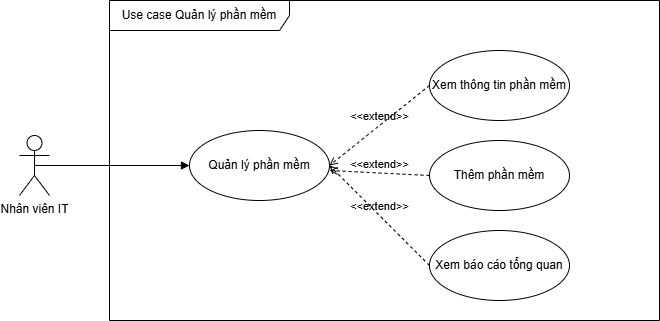
\includegraphics[width=\linewidth]{Images/C5/UseCaseDiagrams/Use-case-Quan-ly-phan-mem.drawio.png}
%     \vspace{5pt}
%     \caption{Use case Quản lý phần mềm}
% \end{figure}
% \begin{table}[H]
%         \centering
%         \caption{Đặc tả Use case Quản lý phần mềm}
%         \begin{tabular}{|p{4cm}|p{10cm}|}
%             \hline
%             Tên use-case & Quản lý phần mềm\\
%             \hline
%             Đối tượng & Nhân viên IT \\
%             \hline
%             Mô tả & Nhân viên IT thực hiện quản lý phần mềm \\
%             \hline
%             Diều kiện kích hoạt & Nhân viên IT bấm nút "Phần mềm" trên giao diện chính của hệ thống \\
%             \hline
%             Tiền điều kiện & Nhân viên IT đã đăng nhập vào hệ thống, có quyền truy cập vào tính năng Quản lý phần mềm. \\
%             \hline
%             Hậu điều kiện & Nhân viên IT thực hiện quản lý phần mềm thành công. \\
%             \hline
%             Luồng tương tác chính & 
%             \begin{enumerate}
%                 \item Nhân viên IT chọn "Phần mềm" ở giao diện chính của hệ thống.
%                 \item Hệ thống hiển thị danh sách các phần mềm.
%                 \item Nhân viên IT chọn phần mềm cần xem chi tiết.
%                 \item Hệ thống hiển thị thông tin chi tiết của phần mềm.
%             \end{enumerate}
%             \\
%             \hline
%             Luồng tương tác thay thế&
            
%             Tại bước 3:
            
%             3.1. Nhân viên IT chọn "Thêm phần mềm" để thêm phần mềm mới.
            
%             3.2. Hệ thống hiển thị giao diện thêm phần mềm.
            
%             3.3. Nhân viên IT nhập thông tin cho phần mềm cần thêm và bấm "Lưu".

%             3.4. Hệ thống kiểm tra và ghi nhận thông tin phần mềm.
%             \newline

%             Tại bước 2:
            
%             2.1. Nhân viên IT chọn "Báo cáo tổng quan".
            
%             2.2. Hệ thống hiển thị báo cáo tổng quan về phần mềm.
%             \\
%             \hline
%             Luồng tương tác ngoại lệ &
            
%             Tại bước 2: Hệ thống lỗi trong việc hiển thị danh sách phần mềm, hệ thống báo lỗi.

%             Tại bước 4: Hệ thống lỗi trong việc hiển thị thông tin phần mềm, hệ thống báo lỗi.

%             Tại bước 2.2: Hệ thống lỗi trong việc hiển thị báo cáo thổng quan về phần mềm, hệ thống báo lỗi.

%             Tại bước 3.4: Hệ thống lỗi trong việc kiểm tra và ghi nhận thông tin phần mềm, hệ thống báo lỗi.
%             \\
%             \hline
%         \end{tabular}
        
%         \label{tab:my_label}
% \end{table}

% \item{ Use case Quản lý giấy phép phần mềm}
% \begin{figure}[H]
%     \centering
%     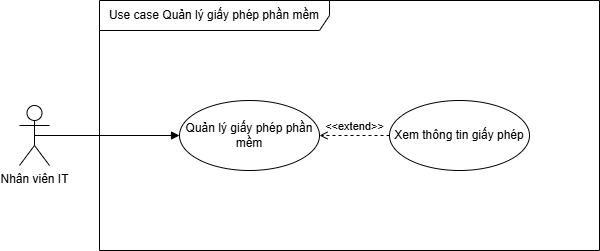
\includegraphics[width=\linewidth]{Images/C5/UseCaseDiagrams/Use-case-Quan-ly-giay-phep-phan-mem.drawio.png}
%     \vspace{5pt}
%     \caption{Use case Quản lý giấy phép phần mềm}
% \end{figure}
% \begin{table}[H]
%         \centering
%         \caption{Đặc tả Use case Quản lý giấy phép phần mềm}
%         \begin{tabular}{|p{4cm}|p{10cm}|}
%             \hline
%             Tên use-case & Quản lý giấy phép phần mềm\\
%             \hline
%             Đối tượng & Nhân viên IT\\
%             \hline
%             Mô tả & Nhân viên IT thực hiện quản lý giấy phép phần mềm. \\
%             \hline
%             Điều kiện kích hoạt & Nhân viên IT bấm vào nút "Giấy phép phần mềm" trên giao diện chính của hệ thống.\\
%             \hline
%             Tiền điều kiện &  Nhân viên IT đã đăng nhập vào hệ thống, có quyền truy cập vào tính năng Quản lý giấy phép phần mềm.\\
%             \hline
%             Hậu điều kiện & Nhân viên IT thực hiện quản lý giấy phép phần mềm thành công \\
%             \hline
%             Luồng tương tác chính & 
%             \begin{enumerate}
%                 \item Nhân viên IT chọn "Giấy phép phần mềm" trên giao diện chính của hệ thống.
%                 \item Hệ thống hiển thị danh sách giấy phép phần mềm.
%                 \item Nhân viên IT chọn giấy phép phần mềm cần xem.
%                 \item Hệ thống hiển thị chi tiết giấy phép phần mềm.
%             \end{enumerate}
%             \\
%             \hline
%             Luồng tương tác thay thế& Không có \\
%             \hline
%             Luồng tương tác ngoại lệ &
%             Tại bước 2: Hệ thống lỗi trong việc hiển thị danh sách giấy phép phần mềm, hệ thống báo lỗi.

%             Tại bước 4: Hệ thống lỗi trong việc hiển thị chi tiết giấy phép phần mềm, hệ thống báo lỗi.
%             \\
%             \hline
%         \end{tabular}
        
%         \label{tab:my_label}
% \end{table}

% \item{ Quản lý cảnh báo}
% \begin{figure}[H]
%     \centering
%     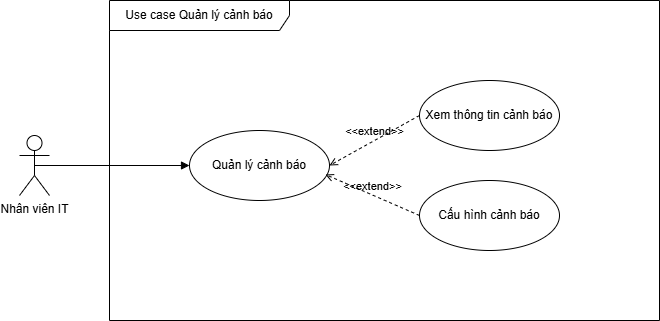
\includegraphics[width=\linewidth]{Images/C5/UseCaseDiagrams/Use-case-Quan-ly-canh-bao.drawio.png}
%     \vspace{5pt}
%     \caption{Use case Quản lý cảnh báo}
% \end{figure}
% \begin{table}[H]
%         \centering
%         \caption{Đặc tả Use case Xem thông tin cảnh báo}
%         \begin{tabular}{|p{4cm}|p{10cm}|}
%             \hline
%             Tên use-case & Xem thông tin cảnh báo\\
%             \hline
%             Đối tượng & Nhân viên IT \\
%             \hline
%             Mô tả & Nhân viên IT thực hiện xem thông tin cảnh báo. \\
%             \hline
%             Diều kiện kích hoạt & Nhân viên IT bấm nút "Cảnh báo" trên giao diện chính của hệ thống \\
%             \hline
%             Tiền điều kiện & Nhân viên IT đã đăng nhập vào hệ thống, có quyền truy cập vào tính năng Quản lý cảnh báo. \\
%             \hline
%             Hậu điều kiện & Nhân viên IT thực hiện xem thông tin cảnh báo thành công. \\
%             \hline
%             Luồng tương tác chính &
%             \begin{enumerate}
%                 \item Nhân viên IT chọn "Cảnh báo" trên giao diện chính của hệ thống.
%                 \item Hệ thống hiển thị danh sách các cảnh báo.
%                 \item Nhân viên IT chọn cảnh báo cần xem chi tiết.
%                 \item Hệ thống hiển chị thông tin chi tiết của cảnh báo.
%             \end{enumerate}\\
%             \hline
%             Luồng tương tác thay thế& Không có \\
%             \hline
%             Luồng tương tác ngoại lệ & 
            
%             Tại bước 2: Hệ thống lỗi trong việc hiển thị danh sách cảnh báo, hệ thống báo lỗi.

%             Tại bước 4: Hệ thống lỗi trong việc hiển thị thông tin cảnh báo, hệ thống báo lỗi.
%             \\
%             \hline
%         \end{tabular}
        
%         \label{tab:my_label}
% \end{table}

% \begin{table}[H]
%         \centering
%         \caption{Đặc tả Use case Cấu hình cảnh báo}
%         \begin{tabular}{|p{4cm}|p{10cm}|}
%             \hline
%             Tên use-case & Cấu hình cảnh báo\\
%             \hline
%             Đối tượng & Nhân viên IT \\
%             \hline
%             Mô tả & b Nhân viên IT thực hiện cấu hình cảnh báo. \\
%             \hline
%             Diều kiện kích hoạt & Nhân viên IT bấm nút "Cấu hình cảnh báo" trên giao diện chính của hệ thống \\
%             \hline
%             Tiền điều kiện & Nhân viên IT đã đăng nhập vào hệ thống, có quyền truy cập vào tính năng Cấu hình cảnh báo. \\
%             \hline
%             Hậu điều kiện & Nhân viên IT thực hiện cấu hình cảnh báo thành công. \\
%             \hline
%             Luồng tương tác chính &
%             \begin{enumerate}
%                 \item Nhân viên IT chọn "Cấu hình cảnh báo" trên giao diện chính của hệ thống (phần Cấu hình).
%                 \item Hệ thống hiển thị giao diện cấu hình cảnh báo.
%                 \item Nhân viên IT thực hiện cấu hình cảnh báo.
%                 \item Hệ thống kiểm tra và lưu cấu hình cảnh báo.
%             \end{enumerate}\\
%             \hline
%             Luồng tương tác thay thế& Không có \\
%             \hline
%             Luồng tương tác ngoại lệ & 
            
%             Tại bước 4: Hệ thống lỗi trong việc kiểm tra và lưu cấu hình cảnh báo, hệ thống báo lỗi.
%             \\
%             \hline
%         \end{tabular}
        
%         \label{tab:my_label}
% \end{table}

% \item{ Quản lý sự cố và bảo trì}
% \begin{figure}[H]
%     \centering
%     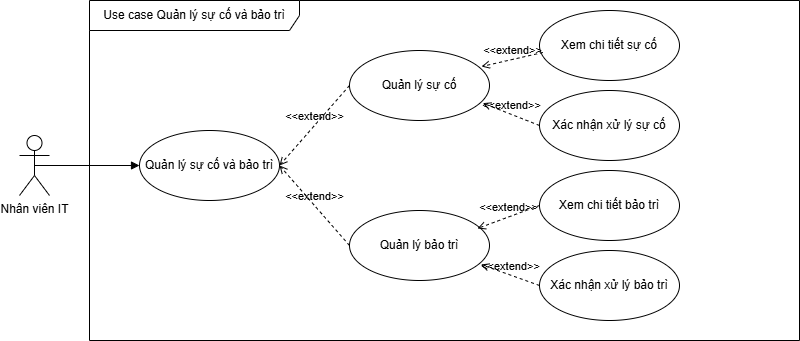
\includegraphics[width=\linewidth]{Images/C5/UseCaseDiagrams/Use-case-Quan-ly-su-co-va-bao-tri.drawio.png}
%     \vspace{5pt}
%     \caption{Use case Quản lý sự cố và bảo trì}
% \end{figure}
% \begin{table}[H]
%         \centering
%         \caption{Đặc tả Use case Quản lý sự cố}
%         \begin{tabular}{|p{4cm}|p{10cm}|}
%             \hline
%             Tên use-case & Quản lý sự cố\\
%             \hline
%             Đối tượng & Nhân viên IT \\
%             \hline
%             Mô tả & b Nhân viên IT thực hiện quản lý sự cố. \\
%             \hline
%             Diều kiện kích hoạt & Nhân viên IT bấm nút "Quản lý sự cố và bảo trì" trên giao diện chính của hệ thống \\
%             \hline
%             Tiền điều kiện & Nhân viên IT đã đăng nhập vào hệ thống, có quyền truy cập vào tính năng Quản lý sự cố. \\
%             \hline
%             Hậu điều kiện & Nhân viên IT thực hiện quản lý sự cố thành công. \\
%             \hline
%             Luồng tương tác chính &
%             \begin{enumerate}
%                 \item Nhân viên IT chọn "Quản lý sự cố và bảo trì" trên giao diện chính của hệ thống và chọn "Danh sách sự cố"
%                 \item Hệ thống hiển thị danh sách sự cố.
%                 \item Nhân viên IT chọn sự cố cần xem chi tiết.
%                 \item Hệ thống hiển thị chi tiết sự cố.
%                 \item Nhân viên IT chọn "Xác nhận đã xử lý" để xác nhận sự cố đã được xử lý.
%                 \item Hệ thống ghi nhận và cập nhật lại trạng thái xử lý.
%             \end{enumerate}\\
%             \hline
%             Luồng tương tác thay thế& Không có \\
%             \hline
%             Luồng tương tác ngoại lệ & 

%             Tại bước 2: Hệ thống lỗi trong việc hiển thị danh sách sự cố, hệ thống báo lỗi.

%             Tại bước 4: Hệ thống lỗi trong việc hiển thị chi tiết sự cố, hệ thống báo lỗi.
            
%             Tại bước 6: Hệ thống lỗi trong việc kiểm tra và ghi nhận cập nhật xử lý sự cố, hệ thống báo lỗi.
%             \\
%             \hline
%         \end{tabular}
        
%         \label{tab:my_label}
% \end{table}

% \begin{table}[H]
%         \centering
%         \caption{Đặc tả Use case Quản lý sự cố}
%         \begin{tabular}{|p{4cm}|p{10cm}|}
%             \hline
%             Tên use-case & Quản lý bảo trì\\
%             \hline
%             Đối tượng & Nhân viên IT \\
%             \hline
%             Mô tả & b Nhân viên IT thực hiện quản lý bảo trì. \\
%             \hline
%             Diều kiện kích hoạt & Nhân viên IT bấm nút "Quản lý sự cố và bảo trì" trên giao diện chính của hệ thống \\
%             \hline
%             Tiền điều kiện & Nhân viên IT đã đăng nhập vào hệ thống, có quyền truy cập vào tính năng Quản lý bảo trì. \\
%             \hline
%             Hậu điều kiện & Nhân viên IT thực hiện quản lý bảo trì thành công. \\
%             \hline
%             Luồng tương tác chính &
%             \begin{enumerate}
%                 \item Nhân viên IT chọn "Quản lý sự cố và bảo trì" trên giao diện chính của hệ thống và chọn "Danh sách yêu cầu bảo trì"
%                 \item Hệ thống hiển thị danh sách yêu cầu bảo trì.
%                 \item Nhân viên IT chọn yêu cầu bảo trì cần xem chi tiết.
%                 \item Hệ thống hiển thị chi tiết yêu cầu bảo trì.
%                 \item Nhân viên IT chọn "Xác nhận hoàn tất" để xác nhận yêu cầu bảo trì đã được xử lý.
%                 \item Hệ thống ghi nhận và cập nhật lại trạng thái xử lý yêu cầu bảo trì.
%             \end{enumerate}\\
%             \hline
%             Luồng tương tác thay thế& Không có \\
%             \hline
%             Luồng tương tác ngoại lệ & 

%             Tại bước 2: Hệ thống lỗi trong việc hiển thị danh sách yêu cầu bảo trì, hệ thống báo lỗi.

%             Tại bước 4: Hệ thống lỗi trong việc hiển thị chi tiết yêu cầu bảo trì, hệ thống báo lỗi.
            
%             Tại bước 6: Hệ thống lỗi trong việc kiểm tra và ghi nhận cập nhật xử lý yêu cầu bảo trì, hệ thống báo lỗi.
%             \\
%             \hline
%         \end{tabular}
        
%         \label{tab:my_label}
% \end{table}

% \item{ Use case Quản lý yêu cầu nâng cấp}
% \begin{figure}[H]
%     \centering
%     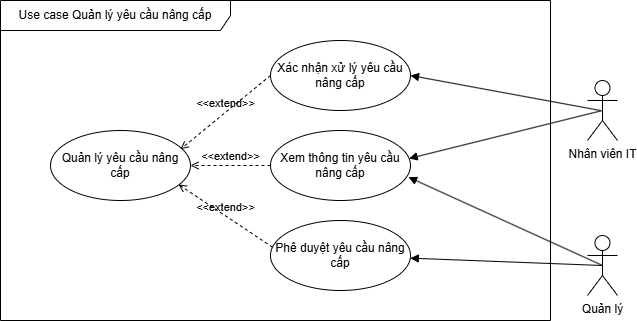
\includegraphics[width=\linewidth]{Images/C5/UseCaseDiagrams/Use-case-Quan-ly-yeu-cau-nang-cap.drawio.png}
%     \vspace{5pt}
%     \caption{Use case Quản lý yêu cầu nâng cấp}
% \end{figure}
% \begin{table}[H]
%         \centering
%         \caption{Đặc tả Use case Xác nhận xử lý yêu cầu nâng cấp}
%         \begin{tabular}{|p{4cm}|p{10cm}|}
%             \hline
%             Tên use-case & Xác nhận xử lý yêu cầu nâng cấp\\
%             \hline
%             Đối tượng & Nhân viên IT \\
%             \hline
%             Mô tả & Nhân viên IT thực hiện xác nhận đã xử lý yêu cầu nâng cấp \\
%             \hline
%             Điều kiện kích hoạt & Nhân viên IT bấm vào nút "Xác nhận xử lý" trên giao diện thông tin chi tiết yêu cầu nâng cấp\\
%             \hline
%             Tiền điều kiện &  Nhân viên IT đã đăng nhập vào hệ thống, có quyền truy cập vào tính năng Quản lý yêu cầu nâng cấp.\\
%             \hline
%             Hậu điều kiện & Nhân viên IT thực hiện xác nhận xử lý yêu cầu nâng cấp thành công \\
%             \hline
%             Luồng tương tác chính & 
%             \begin{enumerate}
%                 \item Nhân viên IT chọn "Yêu cầu nâng cấp" trên giao diện chính của hệ thống.
%                 \item Hệ thống hiển thị danh sách yêu cầu nâng cấp.
%                 \item Nhân viên IT chọn yêu cầu nâng cấp cần xem.
%                 \item Hệ thống hiển thị chi tiết yêu cầu nâng cấp.
%                 \item Nhân viên IT chọn ""Xác nhận xử lý" trên giao diện thông tin chi tiết yêu cầu nâng cấp.
%                 \item Hệ thống kiểm tra và ghi nhận thông tin xác nhận xử lý.
%             \end{enumerate}
%             \\
%             \hline
%             Luồng tương tác thay thế& Không có \\
%             \hline
%             Luồng tương tác ngoại lệ &
%             Tại bước 2: Hệ thống lỗi trong việc hiển thị danh sách yêu cầu nâng cấp, hệ thống báo lỗi.

%             Tại bước 4: Hệ thống lỗi trong việc hiển thị chi tiết yêu cầu nâng cấp, hệ thống báo lỗi.
            
%             Tại bước 6: Hệ thống lỗi trong việc kiểm tra và ghi nhận cập nhật xử lý yêu cầu nâng cấp, hệ thống báo lỗi.
%             \\
%             \hline
%         \end{tabular}
        
%         \label{tab:my_label}
% \end{table}

% \begin{table}[H]
%         \centering
%         \caption{Đặc tả Use case Xem thông tin yêu cầu nâng cấp}
%         \begin{tabular}{|p{4cm}|p{10cm}|}
%             \hline
%             Tên use-case & Xem thông tin yêu cầu nâng cấp\\
%             \hline
%             Đối tượng & Nhân viên IT, Quản lý \\
%             \hline
%             Mô tả & Nhân viên IT, Quản lý thực hiện xem thông tin yêu cầu nâng cấp \\
%             \hline
%             Điều kiện kích hoạt & Nhân viên IT, Quản lý bấm vào nút "Yêu cầu nâng cấp" trên giao diện chính của hệ thống.\\
%             \hline
%             Tiền điều kiện &  Nhân viên IT, Quản lý đã đăng nhập vào hệ thống, có quyền truy cập vào tính năng Quản lý yêu cầu nâng cấp.\\
%             \hline
%             Hậu điều kiện & Nhân viên IT, Quản lý thực hiện xem thông tin yêu cầu nâng cấp thành công \\
%             \hline
%             Luồng tương tác chính & 
%             \begin{enumerate}
%                 \item Nhân viên IT, Quản lý chọn "Yêu cầu nâng cấp" trên giao diện chính của hệ thống.
%                 \item Hệ thống hiển thị danh sách yêu cầu nâng cấp.
%                 \item Nhân viên IT, Quản lý chọn yêu cầu nâng cấp cần xem.
%                 \item Hệ thống hiển thị chi tiết yêu cầu nâng cấp.
%             \end{enumerate}
%             \\
%             \hline
%             Luồng tương tác thay thế& Không có \\
%             \hline
%             Luồng tương tác ngoại lệ &
%             Tại bước 2: Hệ thống lỗi trong việc hiển thị danh sách yêu cầu nâng cấp, hệ thống báo lỗi.

%             Tại bước 4: Hệ thống lỗi trong việc hiển thị chi tiết yêu cầu nâng cấp, hệ thống báo lỗi.
%             \\
%             \hline
%         \end{tabular}
        
%         \label{tab:my_label}
% \end{table}

% \begin{table}[H]
%         \centering
%         \caption{Đặc tả Use case Phê duyệt yêu cầu nâng cấp}
%         \begin{tabular}{|p{4cm}|p{10cm}|}
%             \hline
%             Tên use-case & Phê duyệt yêu cầu nâng cấp\\
%             \hline
%             Đối tượng & Quản lý \\
%             \hline
%             Mô tả & Quản lý thực hiện phê duyệt yêu cầu nâng cấp \\
%             \hline
%             Điều kiện kích hoạt & Quản lý bấm vào nút "Phê duyệt" trên giao diện thông tin chi tiết yêu cầu nâng cấp\\
%             \hline
%             Tiền điều kiện &  Quản lý đã đăng nhập vào hệ thống, có quyền truy cập vào tính năng Quản lý yêu cầu nâng cấp.\\
%             \hline
%             Hậu điều kiện & Quản lý thực hiện phê duyệt yêu cầu nâng cấp thành công \\
%             \hline
%             Luồng tương tác chính & 
%             \begin{enumerate}
%                 \item Quản lý chọn "Yêu cầu nâng cấp" trên giao diện chính của hệ thống.
%                 \item Hệ thống hiển thị danh sách yêu cầu nâng cấp.
%                 \item Quản lý chọn yêu cầu nâng cấp cần xem.
%                 \item Hệ thống hiển thị chi tiết yêu cầu nâng cấp.
%                 \item Quản lý chọn "Phê duyệt" trên giao diện thông tin chi tiết yêu cầu nâng cấp.
%                 \item Hệ thống kiểm tra và ghi nhận thông tin phê duyệt.
%             \end{enumerate}
%             \\
%             \hline
%             Luồng tương tác thay thế& Không có \\
%             \hline
%             Luồng tương tác ngoại lệ &
%             Tại bước 2: Hệ thống lỗi trong việc hiển thị danh sách yêu cầu nâng cấp, hệ thống báo lỗi.

%             Tại bước 4: Hệ thống lỗi trong việc hiển thị chi tiết yêu cầu nâng cấp, hệ thống báo lỗi.
            
%             Tại bước 6: Hệ thống lỗi trong việc kiểm tra và ghi nhận phê duyệt yêu cầu nâng cấp, hệ thống báo lỗi.
%             \\
%             \hline
%         \end{tabular}
        
%         \label{tab:my_label}
% \end{table}

% \item{ Use case Quản lý yêu cầu thanh lý}
% \begin{figure}[H]
%     \centering
%     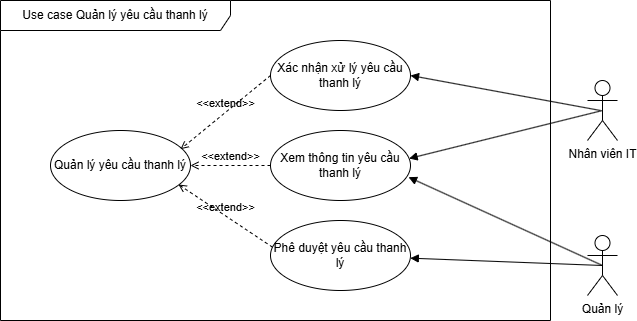
\includegraphics[width=\linewidth]{Images/C5/UseCaseDiagrams/Use-case-Quan-ly-yeu-cau-thanh-ly.drawio.png}
%     \vspace{5pt}
%     \caption{Use case Quản lý yêu cầu thanh lý}
% \end{figure}
% \begin{table}[H]
%         \centering
%         \caption{Đặc tả Use case Xác nhận xử lý yêu cầu thanh lý}
%         \begin{tabular}{|p{4cm}|p{10cm}|}
%             \hline
%             Tên use-case & Xác nhận xử lý yêu cầu thanh lý\\
%             \hline
%             Đối tượng & Nhân viên IT \\
%             \hline
%             Mô tả & Nhân viên IT thực hiện xác nhận đã xử lý yêu cầu thanh lý \\
%             \hline
%             Điều kiện kích hoạt & Nhân viên IT bấm vào nút "Xác nhận xử lý" trên giao diện thông tin chi tiết yêu cầu thanh lý\\
%             \hline
%             Tiền điều kiện &  Nhân viên IT đã đăng nhập vào hệ thống, có quyền truy cập vào tính năng Quản lý yêu cầu thanh lý.\\
%             \hline
%             Hậu điều kiện & Nhân viên IT thực hiện xác nhận xử lý yêu cầu thanh lý thành công \\
%             \hline
%             Luồng tương tác chính & 
%             \begin{enumerate}
%                 \item Nhân viên IT chọn "Yêu cầu thanh lý" trên giao diện chính của hệ thống.
%                 \item Hệ thống hiển thị danh sách yêu cầu thanh lý.
%                 \item Nhân viên IT chọn yêu cầu thanh lý cần xem.
%                 \item Hệ thống hiển thị chi tiết yêu cầu thanh lý.
%                 \item Nhân viên IT chọn ""Xác nhận xử lý" trên giao diện thông tin chi tiết yêu cầu thanh lý.
%                 \item Hệ thống kiểm tra và ghi nhận thông tin xác nhận xử lý.
%             \end{enumerate}
%             \\
%             \hline
%             Luồng tương tác thay thế& Không có \\
%             \hline
%             Luồng tương tác ngoại lệ &
%             Tại bước 2: Hệ thống lỗi trong việc hiển thị danh sách yêu cầu thanh lý, hệ thống báo lỗi.

%             Tại bước 4: Hệ thống lỗi trong việc hiển thị chi tiết yêu cầu thanh lý, hệ thống báo lỗi.
            
%             Tại bước 6: Hệ thống lỗi trong việc kiểm tra và ghi nhận cập nhật xử lý yêu cầu thanh lý, hệ thống báo lỗi.
%             \\
%             \hline
%         \end{tabular}
        
%         \label{tab:my_label}
% \end{table}

% \begin{table}[H]
%         \centering
%         \caption{Đặc tả Use case Xem thông tin yêu cầu thanh lý}
%         \begin{tabular}{|p{4cm}|p{10cm}|}
%             \hline
%             Tên use-case & Xem thông tin yêu cầu thanh lý\\
%             \hline
%             Đối tượng & Nhân viên IT, Quản lý \\
%             \hline
%             Mô tả & Nhân viên IT, Quản lý thực hiện xem thông tin yêu cầu thanh lý \\
%             \hline
%             Điều kiện kích hoạt & Nhân viên IT, Quản lý bấm vào nút "Yêu cầu thanh lý" trên giao diện chính của hệ thống.\\
%             \hline
%             Tiền điều kiện &  Nhân viên IT, Quản lý đã đăng nhập vào hệ thống, có quyền truy cập vào tính năng Quản lý yêu cầu thanh lý.\\
%             \hline
%             Hậu điều kiện & Nhân viên IT, Quản lý thực hiện xem thông tin yêu cầu thanh lý thành công \\
%             \hline
%             Luồng tương tác chính & 
%             \begin{enumerate}
%                 \item Nhân viên IT, Quản lý chọn "Yêu cầu thanh lý" trên giao diện chính của hệ thống.
%                 \item Hệ thống hiển thị danh sách yêu cầu thanh lý.
%                 \item Nhân viên IT, Quản lý chọn yêu cầu thanh lý cần xem.
%                 \item Hệ thống hiển thị chi tiết yêu cầu thanh lý.
%             \end{enumerate}
%             \\
%             \hline
%             Luồng tương tác thay thế& Không có \\
%             \hline
%             Luồng tương tác ngoại lệ &
%             Tại bước 2: Hệ thống lỗi trong việc hiển thị danh sách yêu cầu thanh lý, hệ thống báo lỗi.

%             Tại bước 4: Hệ thống lỗi trong việc hiển thị chi tiết yêu cầu thanh lý, hệ thống báo lỗi.
%             \\
%             \hline
%         \end{tabular}
        
%         \label{tab:my_label}
% \end{table}

% \begin{table}[H]
%         \centering
%         \caption{Đặc tả Use case Phê duyệt yêu cầu thanh lý}
%         \begin{tabular}{|p{4cm}|p{10cm}|}
%             \hline
%             Tên use-case & Phê duyệt yêu cầu thanh lý\\
%             \hline
%             Đối tượng & Quản lý \\
%             \hline
%             Mô tả & Quản lý thực hiện phê duyệt yêu cầu thanh lý \\
%             \hline
%             Điều kiện kích hoạt & Quản lý bấm vào nút "Phê duyệt" trên giao diện thông tin chi tiết yêu cầu thanh lý\\
%             \hline
%             Tiền điều kiện &  Quản lý đã đăng nhập vào hệ thống, có quyền truy cập vào tính năng Quản lý yêu cầu thanh lý.\\
%             \hline
%             Hậu điều kiện & Quản lý thực hiện phê duyệt yêu cầu thanh lý thành công \\
%             \hline
%             Luồng tương tác chính & 
%             \begin{enumerate}
%                 \item Quản lý chọn "Yêu cầu thanh lý" trên giao diện chính của hệ thống.
%                 \item Hệ thống hiển thị danh sách yêu cầu thanh lý.
%                 \item Quản lý chọn yêu cầu thanh lý cần xem.
%                 \item Hệ thống hiển thị chi tiết yêu cầu thanh lý.
%                 \item Quản lý chọn "Phê duyệt" trên giao diện thông tin chi tiết yêu cầu thanh lý.
%                 \item Hệ thống kiểm tra và ghi nhận thông tin phê duyệt.
%             \end{enumerate}
%             \\
%             \hline
%             Luồng tương tác thay thế& Không có \\
%             \hline
%             Luồng tương tác ngoại lệ &
%             Tại bước 2: Hệ thống lỗi trong việc hiển thị danh sách yêu cầu thanh lý, hệ thống báo lỗi.

%             Tại bước 4: Hệ thống lỗi trong việc hiển thị chi tiết yêu cầu thanh lý, hệ thống báo lỗi.
            
%             Tại bước 6: Hệ thống lỗi trong việc kiểm tra và ghi nhận phê duyệt yêu cầu thanh lý, hệ thống báo lỗi.
%             \\
%             \hline
%         \end{tabular}
        
%         \label{tab:my_label}
% \end{table}

% \item{ Use case Quản lý đơn đặt hàng}
% \begin{figure}[H]
%     \centering
%     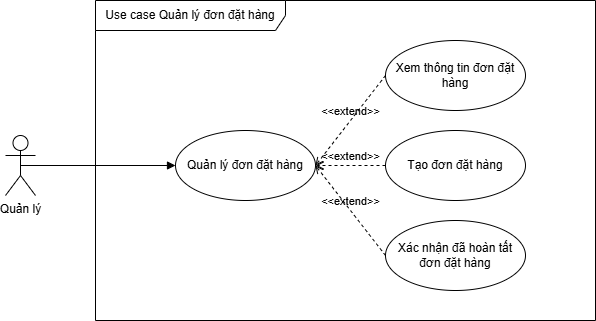
\includegraphics[width=\linewidth]{Images/C5/UseCaseDiagrams/Use-case-Quan-ly-don-dat-hang.drawio.png}
%     \vspace{5pt}
%     \caption{Use case Quản lý đơn đặt hàng}
% \end{figure}

% \begin{table}[H]
%         \centering
%         \caption{Đặc tả Use case Quản lý đơn đặt hàng}
%         \begin{tabular}{|p{4cm}|p{10cm}|}
%             \hline
%             Tên use-case & Quản lý đơn đặt hàng\\
%             \hline
%             Đối tượng & Quản lý \\
%             \hline
%             Mô tả & Quản lý có thể thực hiện quản lý đơn đặt hàng \\
%             \hline
%             Diều kiện kích hoạt & Quản lý chọn "Đơn đặt hàng" trên giao diện chính của hệ thống \\
%             \hline
%             Tiền điều kiện & Quản lý đã đăng nhập vào hệ thống, có quyền truy cập vào tính năng Quản lý đơn đặt hàng \\
%             \hline
%             Hậu điều kiện & Quản lý có thể thực hiện quản lý đơn đặt hàng thành công \\
%             \hline
%             Luồng tương tác chính &
%             \begin{enumerate}
%                 \item Quản lý chọn vào mục "Đơn đặt hàng".
%                 \item Hệ thống hiển thị danh sách đơn đặt hàng.
%                 \item Quản lý chọn đơn đặt hàng cần xem thông tin.
%                 \item Hệ thống hiện thị thông tin về đơn đặt hàng.
%                 \item Quản lý chọn "Xác nhận đã hoàn tất" để xác nhận đơn hàng đã hoàn tất.
%                 \item Hệ thống kiểm tra và ghi nhận hoàn tất đơn hàng.
%             \end{enumerate}\\
%             \hline
%             Luồng tương tác thay thế&  
            
%             Tại bước 2: 
                
%             2.1 Nếu muốn thêm đơn đặt hàng mới, chọn "Thêm đơn đặt hàng"
            
%             2.2. Quản lý nhập thông tin cho đơn đặt hàng và bấm "Đặt hàng"
            
%             2.3. Hệ thống kiểm tra và ghi nhận đơn đặt hàng.
                  
%             \\
%             \hline
%             Luồng tương tác ngoại lệ &

%             Tại bước 2: Hệ thống lỗi trong việc hiển thị danh sách đơn đặt hàng, hệ thống báo lỗi.

%             Tại bước 4: Hệ thống lỗi trong việc hiển thị chi tiết đơn đặt hàng, hệ thống báo lỗi.
            
%             Tại bước 6: Hệ thống lỗi trong việc kiểm tra và ghi nhận cập nhật hoàn tất đơn đặt hàng, hệ thống báo lỗi.
%             \\
%             \hline
%         \end{tabular}
        
%         \label{tab:my_label}
% \end{table}

% % \item{ Use case Quản lý tài chính}
% % \begin{figure}[H]
% %     \centering
% %     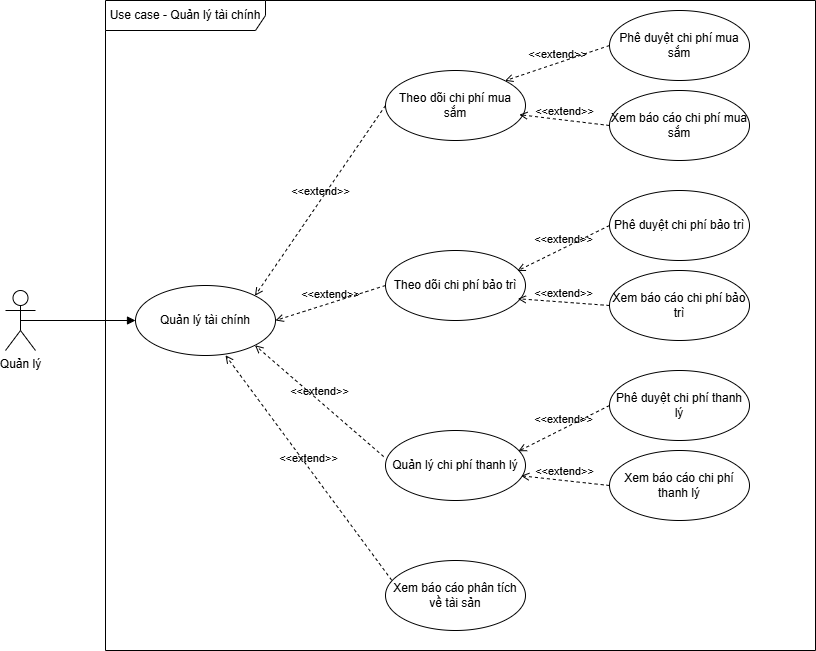
\includegraphics[width=\linewidth]{Images/C5/UseCaseDiagrams/Use-case-Quan-ly-tai-chinh.drawio.png}
% %     \vspace{5pt}
% %     \caption{Use case Quản lý tài chính}
% % \end{figure}
% % \begin{table}[H]
% %         \centering
% %         \begin{tabular}{|p{4cm}|p{10cm}|}
% %             \hline
% %             Tên use-case & Theo dõi chi phí mua sắm\\
% %             \hline
% %             Đối tượng & Quản lý \\
% %             \hline
% %             Mô tả & Quản lý thực hiện theo dõi chi phí mua sắm. \\
% %             \hline
% %             Diều kiện kích hoạt & Quản lý chọn vào "Chi phí mua sắm" trên giao diện quản lý tài chính \\
% %             \hline
% %             Tiền điều kiện & Quản lý đã đăng nhập vào hệ thống, có quyền truy cập vào tính năng Quản lý tài chính. \\
% %             \hline
% %             Hậu điều kiện & Quản lý thực hiện theo dõi chi phí mua sắm thành công. \\
% %             \hline
% %             Luồng tương tác chính &
% %             \begin{enumerate}
% %                 \item Quản lý chọn vào "Tài chính" trên giao diện chính của hệ thống.
% %                 \item Hệ thống hiển thị giao diện quản lý tài chính.
% %                 \item Quản lý chọn vào "Chi phí mua sắm".
% %                 \item Hệ thống hiển thị danh sách chi phí mua sắm.
% %                 \item Quản lý chọn chi phí mua sắm cần quản lý.
% %                 \item Hệ thống hiển thị chi tiết chi phí mua sắm.
% %                 \item Quản lý chọn "Phê duyệt" để phê duyệt chi phí mua sắm.
% %             \end{enumerate}
% %             \\
% %             \hline
% %             Luồng tương tác thay thế& 
% %             Tại bước 3:
% %             3.1. Quản lý chọn "Báo cáo chi phí mua sắm".
% %             3.2. Hệ thống hiển thị báo cáo về chi phí mua sắm.
% %             \\
% %             \hline
% %             Luồng tương tác ngoại lệ &
% %             Tại bước 4: Hệ thống lỗi trong việc hiển thị danh sách chi phí mua sắm, hệ thống báo lỗi.

% %             Tại bước 6: Hệ thống lỗi trong việc hiển thị chi tiết chi phí mua sắm, hệ thống báo lỗi.
            
% %             Tại bước 3.2: Hệ thống lỗi trong việc hiển thị báo cáo chi phí mua sắm, hệ thống báo lỗi.
% %             \\
% %             \hline
% %         \end{tabular}
% %         \caption{Đặc tả Use case Theo dõi chi phí mua sắm}
% %         \label{tab:my_label}
% % \end{table}

% % \begin{table}[H]
% %         \centering
% %         \begin{tabular}{|p{4cm}|p{10cm}|}
% %             \hline
% %             Tên use-case & Theo dõi chi phí bảo trì\\
% %             \hline
% %             Đối tượng & Quản lý \\
% %             \hline
% %             Mô tả & Quản lý thực hiện theo dõi chi phí bảo trì. \\
% %             \hline
% %             Diều kiện kích hoạt & Quản lý chọn vào "Chi phí bảo trì" trên giao diện quản lý tài chính.\\
% %             \hline
% %             Tiền điều kiện & Quản lý đã đăng nhập vào hệ thống, có quyền truy cập vào tính năng Quản lý tài chính. \\
% %             \hline
% %             Hậu điều kiện & Quản lý thực hiện theo dõi chi phí bảo trì thành công. \\
% %             \hline
% %             Luồng tương tác chính &
% %             \begin{enumerate}
% %                 \item Quản lý chọn vào "Tài chính" trên giao diện chính của hệ thống.
% %                 \item Hệ thống hiển thị giao diện quản lý tài chính.
% %                 \item Quản lý chọn vào "Chi phí bảo trì".
% %                 \item Hệ thống hiển thị danh sách chi phí bảo trì.
% %                 \item Quản lý chọn chi phí bảo trì cần quản lý.
% %                 \item Hệ thống hiển thị chi tiết chi phí bảo trì.
% %                 \item Quản lý chọn "Phê duyệt" để phê duyệt chi phí bảo trì.
% %             \end{enumerate}
% %             \\
% %             \hline
% %             Luồng tương tác thay thế& 
% %             Tại bước 3:
% %             3.1. Quản lý chọn "Báo cáo chi phí bảo trì".
% %             3.2. Hệ thống hiển thị báo cáo về chi phí bảo trì.
% %             \\
% %             \hline
% %             Luồng tương tác ngoại lệ &
% %             Tại bước 4: Hệ thống lỗi trong việc hiển thị danh sách chi phí bảo trì, hệ thống báo lỗi.

% %             Tại bước 6: Hệ thống lỗi trong việc hiển thị chi tiết chi phí bảo trì, hệ thống báo lỗi.
            
% %             Tại bước 3.2: Hệ thống lỗi trong việc hiển thị báo cáo chi phí bảo trì, hệ thống báo lỗi.
% %             \\
% %             \hline
% %         \end{tabular}
% %         \caption{Đặc tả Use case Theo dõi chi phí bảo trì}
% %         \label{tab:use_case_maintenance}
% % \end{table}

% % \begin{table}[H]
% %         \centering
% %         \begin{tabular}{|p{4cm}|p{10cm}|}
% %             \hline
% %             Tên use-case & Quản lý chi phí thanh lý\\
% %             \hline
% %             Đối tượng & Quản lý \\
% %             \hline
% %             Mô tả & Quản lý thực hiện theo dõi và quản lý chi phí thanh lý. \\
% %             \hline
% %             Diều kiện kích hoạt & Quản lý chọn vào "Chi phí thanh lý" trên giao diện quản lý tài chính. \\
% %             \hline
% %             Tiền điều kiện & Quản lý đã đăng nhập vào hệ thống, có quyền truy cập vào tính năng Quản lý tài chính. \\
% %             \hline
% %             Hậu điều kiện & Quản lý thực hiện theo dõi và quản lý chi phí thanh lý thành công. \\
% %             \hline
% %             Luồng tương tác chính &
% %             \begin{enumerate}
% %                 \item Quản lý chọn vào "Tài chính" trên giao diện chính của hệ thống.
% %                 \item Hệ thống hiển thị giao diện quản lý tài chính.
% %                 \item Quản lý chọn vào "Chi phí thanh lý".
% %                 \item Hệ thống hiển thị danh sách chi phí thanh lý.
% %                 \item Quản lý chọn chi phí thanh lý cần quản lý.
% %                 \item Hệ thống hiển thị chi tiết chi phí thanh lý.
% %                 \item Quản lý chọn "Phê duyệt" để phê duyệt chi phí thanh lý.
% %             \end{enumerate}
% %             \\
% %             \hline
% %             Luồng tương tác thay thế& 
% %             Tại bước 3:
% %             3.1. Quản lý chọn "Báo cáo chi phí thanh lý".
% %             3.2. Hệ thống hiển thị báo cáo về chi phí thanh lý.
% %             \\
% %             \hline
% %             Luồng tương tác ngoại lệ &
% %             Tại bước 4: Hệ thống lỗi trong việc hiển thị danh sách chi phí thanh lý, hệ thống báo lỗi.

% %             Tại bước 6: Hệ thống lỗi trong việc hiển thị chi tiết chi phí thanh lý, hệ thống báo lỗi.
            
% %             Tại bước 3.2: Hệ thống lỗi trong việc hiển thị báo cáo chi phí thanh lý, hệ thống báo lỗi.
% %             \\
% %             \hline
% %         \end{tabular}
% %         \caption{Đặc tả Use case Quản lý chi phí thanh lý}
% %         \label{tab:use_case_disposal}
% % \end{table}

% % \begin{table}[H]
% %         \centering
% %         \begin{tabular}{|p{4cm}|p{10cm}|}
% %             \hline
% %             Tên use-case & Xem báo cáo và phân tích về tài sản\\
% %             \hline
% %             Đối tượng & Quản lý \\
% %             \hline
% %             Mô tả & Quản lý thực hiện xem báo cáo và phân tích về tài sản. \\
% %             \hline
% %             Diều kiện kích hoạt & Quản lý chọn vào "Báo cáo về tài sản" trên giao diện quản lý tài chính. \\
% %             \hline
% %             Tiền điều kiện & Quản lý đã đăng nhập vào hệ thống, có quyền truy cập vào tính năng Quản lý tài chính. \\
% %             \hline
% %             Hậu điều kiện & Quản lý thực hiện xem báo cáo và phân tích về tài sản thành công. \\
% %             \hline
% %             Luồng tương tác chính &
% %             \begin{enumerate}
% %                 \item Quản lý chọn vào "Tài chính" trên giao diện chính của hệ thống.
% %                 \item Hệ thống hiển thị giao diện quản lý tài chính.
% %                 \item Quản lý chọn vào "Báo cáo về tài sản".
% %                 \item Hệ thống hiển thị báo cáo và phân tích về tài sản.

% %             \end{enumerate}
% %             \\
% %             \hline
% %             Luồng tương tác thay thế& 
% %             Không có
% %             \\
% %             \hline
% %             Luồng tương tác ngoại lệ &
% %             Tại bước 4: Hệ thống lỗi trong việc hiển thị báo cáo và phân tích về tài sản, hệ thống báo lỗi.
% %             \\
% %             \hline
% %         \end{tabular}
% %         \caption{Đặc tả Use case Xem báo cáo và phân tích về tài sản}
% %         \label{tab:use_case_disposal}
% % \end{table}

% \item{ Use case Quản lý cấu hình hệ thống}
% \begin{figure}[H]
%     \centering
%     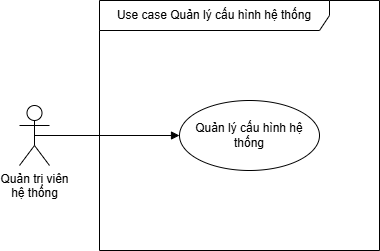
\includegraphics[width=0.7\linewidth]{Images/C5/UseCaseDiagrams/Use-case-Quan-ly-cau-hinh-he-thong.drawio.png}
%     \vspace{15pt}
%     \caption{Use case Quản lý cấu hình hệ thống}
% \end{figure}
% \begin{table}[H]
%         \centering
%         \caption{Đặc tả Use case Quản lý cấu hình hệ thống}
%         \begin{tabular}{|p{4cm}|p{10cm}|}
%             \hline
%             Tên use-case & Quản lý cấu hình hệ thống\\
%             \hline
%             Đối tượng & Quản trị viên hệ thống\\
%             \hline
%             Mô tả & Quản trị viên hệ thống thực hiện quản lý cấu hình hệ thống. \\
%             \hline
%             Điều kiện kích hoạt & Quản trị viên hệ thống chọn vào "Cấu hình chung" trên giao diện chính của hệ thống.\\
%             \hline
%             Tiền điều kiện & Quản trị viên hệ thống đã đăng nhập vào hệ thống, có quyền truy cập vào tính năng Quản lý cấu hình hệ thống. \\
%             \hline
%             Hậu điều kiện & Quản trị viên hệ thống thực hiện quản lý cấu hình hệ thống thành công. \\
%             \hline
%             Luồng tương tác chính & 
%             \begin{enumerate}
%                 \item Quản trị viên hệ thống chọn "Cấu hình chung" trên giao diện chính của hệ thống.
%                 \item Hệ thống hiển thị giao diện cấu hình hệ thống.
%                 \item Quản trị viên hệ thống thực hiện cấu hình hệ thống.
%                 \item Hệ thống kiểm tra và ghi nhận cấu hình.
%             \end{enumerate}
%             \\
%             \hline
%             Luồng tương tác thay thế& Không có \\
%             \hline
%             Luồng tương tác ngoại lệ &
%             Tại bước 4: Hệ thống lỗi trong việc kiểm tra và ghi nhận cấu hình, hệ thống báo lỗi.
%             \\
%             \hline
%         \end{tabular}
        
%         \label{tab:my_label}
% \end{table}

% \end{itemize}

% \subsection{ Giải pháp công nghệ}

% \subsubsection{ Thu thập dữ liệu thời gian thực}
% \begin{enumerate}
%     \item \textbf{Dữ liệu thời gian thực}:
%     \begin{itemize}[label=--]
%         \item \textbf{Dữ liệu thời gian thực (real-time data)}: là dữ liệu được tạo ra và xử lý ngay lập tức, phản ánh trạng thái hiện tại của một hệ thống, sự kiện hoặc hiện tượng. Đặc trưng của loại dữ liệu này là tính tức thời, yêu cầu  phải được xử lý và sử dụng ngay trong thời điểm phát sinh để đảm bảo giá trị và ý nghĩa.\cite{rtd}
%         % \item Tầm quan trọng: 
%         % \begin{itemize}
%         %     \item Ra quyết định nhanh chóng và chính xác
%         %     \item Phản ứng nhanh chóng với sự thay đổi
%         %     \item Cải thiện trải nghiệm người dùng
%         %     \item Tối ưu hóa hiệu quả hoạt động
%         %     \item Nâng cao khả năng cạnh tranh
%         % \end{itemize}
%         \item \textbf{Đặc điểm nổi bật:} 
%         \begin{itemize}[label=\textbullet]
%             \item Tính thức thời: Dữ liệu được tạo ra và xử lý ngay lập tức, thông tin phản ánh trạng thái hiện tại của hệ thống, sự kiện hoặc hiện tượng. Ví dụ: Lượt truy cập website, chỉ số cảm biến từ IoT,...
%             \item Tính liên tục: Dữ liệu được tạo ra liên tục tạo thành một luồng dữ liệu không ngừng, điều này yêu cầu hệ thống phải hoạt động liên tục và ổn định. Ví dụ: nhật ký sự kiện hệ thống
%             \item Tính biến động: dữ liệu có thể thay đổi nhanh chóng và khó dự đoán, điều này yêu cầu hệ thống phải xử lý linh hoạt, thích ứng với sự thay đổi. Ví dụ như: giá cả hàng hóa, giá cổ phiếu biến động trên thị trường chứng khoán.
%             \item Tính ngắn hạn: Giá trị dữ liệu chỉ có ý nghĩa trong thời gian ngắn, dữ liệu cũ có thể bị loại bỏ hoặc lưu trữ với mức độ ưu tiên thấp hơn. Ví dụ như: cảnh báo của hệ thống, định vị, các thông báo. 
%         \end{itemize}
%         \item \textbf{Phân loại dữ liệu thời gian thực}\cite{trtd}:
%         \begin{table}[H]
%         \centering
%         \caption{Loại dữ liệu thời gian thực}
%         \begin{tabular}{|p{2cm}|p{5.5cm}|p{5.5cm}|}
%             \hline
%             \textbf{Đặc điểm} & \textbf{Event Data} & \textbf{Streaming Data} \\
%             \hline
%             Bản chất &
%                 Là dữ liệu gắn nhãn thời gian không đều đặn, được tạo ra khi một sự kiện cụ thể xảy ra. Mỗi sự kiện mang thông tin về sự thay đổi trạng thái của hệ thống
%             &  Là dữ liệu gắn nhãn thời gian đều đặn, được tạo ra dưới dạng một luồng không ngừng, phản ánh trạng thái động của hệ thống. Ví dụ: cách mỗi giây\\
%             \hline
%            Tính chất & Mang tính chất "thời điểm", gắn liền với một mốc thời gian cụ thể &
%            Mang tính chất "thời gian", liên tục thay đổi theo thời gian.\\
%             \hline
%             Cấu trúc & Thường có cấu trúc rõ ràng, chứa thông tin về loại sự kiện, thời gian, đối tượng liên quan,... & Có thể có cấu trúc hoặc không cấu trúc. \\
%             \hline
%             Ví dụ & \begin{itemize}
%                 \item Khách hàng đặt hàng trên Website (sự kiện "đặt hàng")
%                 \item Hệ thống cảnh báo lỗi (sự kiện "lỗi hệ thống")
%             \end{itemize} & \begin{itemize}
%                 \item Dữ liệu cảm biến từ thiết bị IoT
%                 \item Nhật ký sự kiện hệ thống
%                 \item Luồng video từ camera giám sát.
%             \end{itemize}
%             \\
%             \hline
%         \end{tabular}
        
%         \label{tab:my_label}
%     \end{table}
%     \end{itemize}
%        \item \textbf{Apache Kafka trong thu thập dữ liệu thời gian thực}
%         \begin{enumerate}
%             \item \textbf{Các thành phần của Kafka}
%             \begin{figure}[H]
%                 \centering
%                 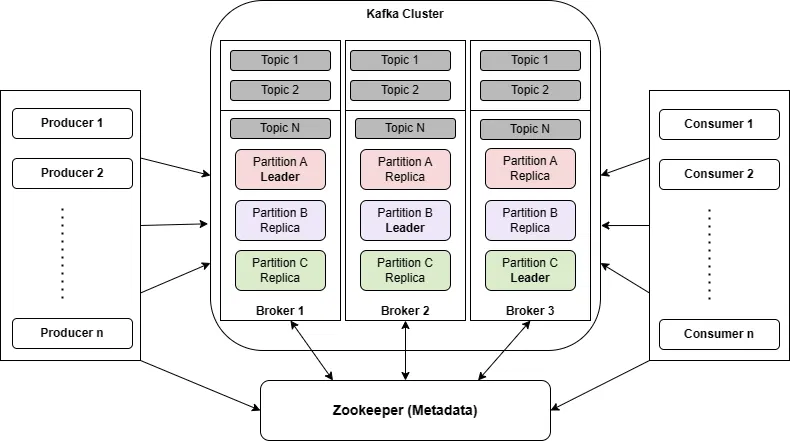
\includegraphics[width=\linewidth]{Images/Kafka/KafkaArchitecture.png}
%                 \vspace{5pt}
%                 \caption{Kiến trúc Kafka\\ Nguồn: 200lab.io, truy cập vào ngày 01/05/2025}
%             \end{figure}
%             \begin{enumerate}
%         \item \textbf{Kafka Events}\\
%         Một Kafka event (sự kiện) còn được gọi là record (bản ghi) hoặc message (thông điệp). Việc sử dụng 3 thuật ngữ event, record và message mang nghĩa tương đương nhau. Hay chỉ đơn giản nó là đơn vị dữ liệu cơ bản trong Kafka, là một mảng byte không có định dạng cụ thể.
    
%         Việc đọc và ghi dữ liệu trong Kafka thực hiện thông qua event. Mỗi event chứa một key (khoá), value (giá trị) và metadata (nếu có).
%     \\
%     \{\\
%     key: "ID",\\
%     value: "2433.544",\\
%     timestamp: "Feb. 12, 2024, at 20:06 p.m."\\
%     \}
%         \item \textbf{Kafka Topics}:
%         \begin{itemize}[label=--]
%         \item Các event được tổ chức và lưu trữ lâu dài trong các topics (chủ đề). Có thể coi một topic ví như một thư mục (folder) trong hệ thống tập tin (filesystem), còn mỗi event là một tập tin (file) nằm bên trong thư mục đó.
%         \item Hình dưới cho thấy một topic có 4 partitions, với phần ghi được thêm vào cuối mỗi partition. Kafka cung cấp khả năng dự phòng (redundancy) và khả năng mở rộng (scalability) thông qua các partitions. Mỗi partition có thể được lưu trữ trên một máy chủ khác nhau, điều đó có nghĩa là một topic có thể được mở rộng theo chiều ngang trên nhiều máy chủ để cung cấp hiệu suất vượt xa khả năng của một máy chủ.
%         \end{itemize}
%         \begin{figure}[H]
%             \centering
%             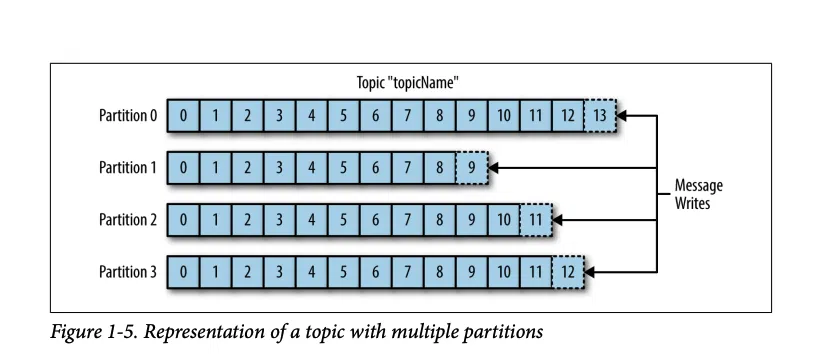
\includegraphics[width=\linewidth]{Images/Kafka/KafkaTopic.png}
%             \vspace{5pt}
%             \caption{Kafka Topic\\ Nguồn: 200lab.io, truy cập vào ngày 01/05/2025}
%         \end{figure}
        
%         \item \textbf{Kafka Brokers và Kafka Clusters}
%         \begin{itemize}[label=--]
%            \item Kafka được chạy dưới dạng một \textbf{Kafka cluster} gồm một hoặc nhiều \textbf{Kafka server} có thể mở rộng trên nhiều data center hoặc cloud. Một Kafka server này tạo thành lớp lưu trữ, được gọi là\textbf{ Kafka broker}.
%             \item \textbf{Brokers} chịu trách nhiệm quản lý bộ lưu trữ, xử lý các yêu cầu đọc và ghi cũng như sao chép dữ liệu trên toàn cluster (cụm).
%             \item Trong mỗi cluster sẽ có một broker sẽ hoạt động như một \textbf{cluster controller} (bộ điều khiển cụm), chịu trách nhiệm chỉ định phân vùng cho brokers và theo dõi lỗi của brokers.
%         \end{itemize}
%         \item \textbf{ Kafka Partitions và Kafka Replication}
%         \begin{itemize}[label=--]
%             \item Các \textbf{topic} được chia thành các \textbf{partitions} (phân vùng), là \textbf{đơn vị cơ bản} của tính song song và phân phối trong Kafka. Mỗi phân vùng được lưu trữ trên \textbf{một broker duy nhất} và nhiều phân vùng cho phép mở rộng quy mô theo chiều ngang và cải thiện hiệu suất.
%              \item Mỗi event trong một partition được gán một \textbf{offset} duy nhất, bắt đầu từ 0 cho event đầu tiên trong partition và tăng dần một cho mỗi event tiếp theo. Offset được sử dụng để xác định vị trí của event trong một partition.
%             \item Kafka đảm bảo độ bền của dữ liệu bằng cách sao chép dữ liệu (replication) trên nhiều brokers. Mỗi partition có thể có một hoặc nhiều \textbf{replica (bản sao)} trên các brokers khác nhau, ngăn ngừa mất dữ liệu trong trường hợp broker lỗi.
%             \begin{figure}[H]
%                 \centering
%                 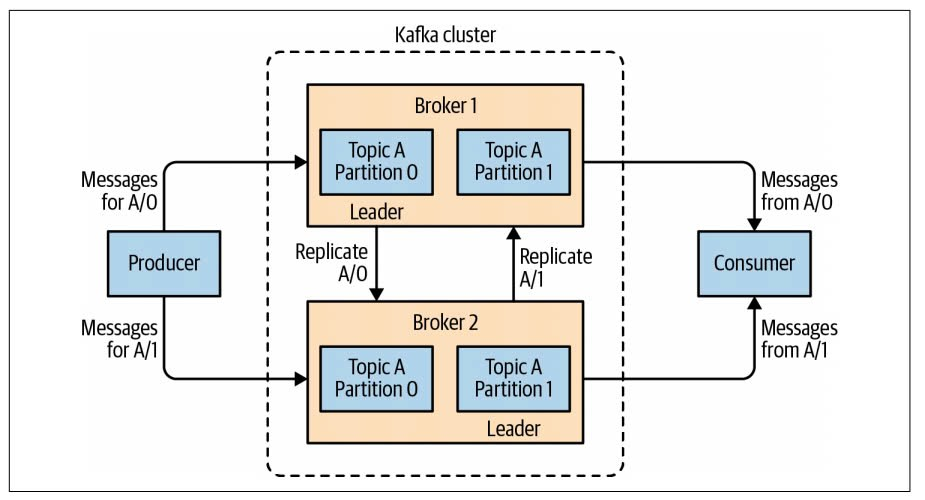
\includegraphics[width=\linewidth]{Images/Kafka/kafkacluster.png}
%                 \vspace{5pt}
%                 \caption{Kafka Cluster\\ Nguồn: 200lab.io, truy cập vào ngày 01/05/2025}
%             \end{figure}
%             \item Mỗi partition có một broker được chỉ định làm \textbf{leader}, nắm quyền sở hữu partition đó, trong khi các \textbf{brokers} còn lại lưu trữ các \textbf{replicas} (bản sao) của phân vùng đó được gọi là \textbf{followers}.
%             Nếu leader broker xảy ra lỗi, một trong những followers có dữ liệu cập nhật sẽ được chọn làm leader mới. Quá trình này được gọi là leader failover (chuyển đổi dự phòng lãnh đạo), nhằm đảm bảo tính khả dụng của dữ liệu.
%         \end{itemize}
%         \item \textbf{Kafka Producers}
%             \begin{itemize}[label=--]
%                 \item \textbf{Kafka Producer} là một client appication (ứng dụng khách), \textbf{publish} (xuất bản) event vào một topic cụ thể trong Kafka và luôn ghi vào \textbf{leader broker}. Theo mặc định, producers không quan tâm tới event được ghi ở partition nào mà sẽ publish đều event trên tất cả partition của một topic. Trong vài trường hợp, một producer sẽ gửi trực tiếp event tới các partition cụ thể.
%                 \item \textbf{Producers} kết nối tới \textbf{Kafka Brokers} thông qua giao thức mạng TCP. Đây là kết nối hai chiều (bi-directional connection).
%             \end{itemize}
%         \begin{figure}[H]
%             \centering
%             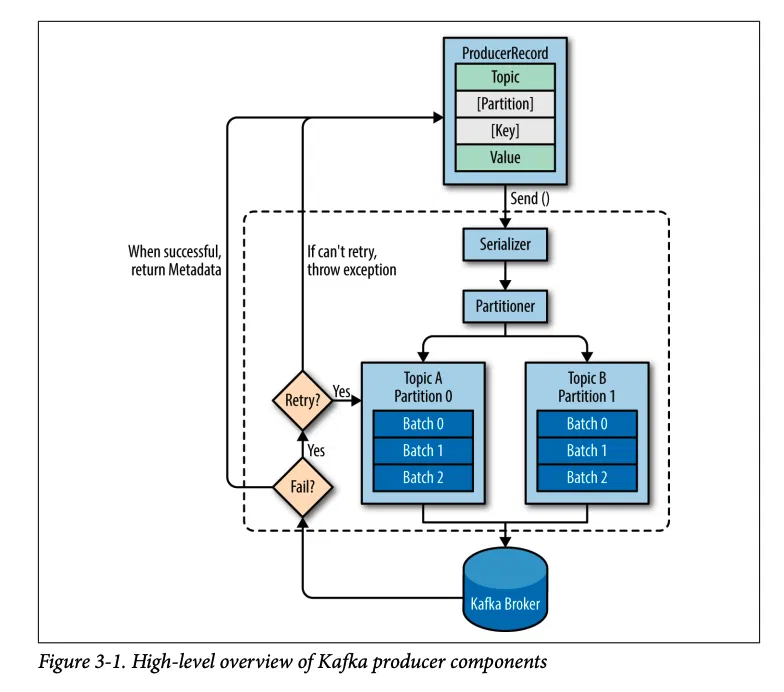
\includegraphics[width=0.7\linewidth]{Images/Kafka/KafkaProducer.png}
%             \vspace{5pt}
%             \caption{Kafka Producer\\ Nguồn: 200lab.io, truy cập vào ngày 01/05/2025}
%         \end{figure}
%         Quá trình gửi event như sau :
%         \begin{itemize}[label=--]
%             \item Tạo produceRecord
%             \item Serializer: Trước khi gửi ProducerRecord qua network, producer sẽ serialize (tuần tự hoá) key và value thành ByteArrays (mảng các bytes).
%             \item Xác định số Partitions: Nếu chúng ta chỉ định sẵn partition thì partitioner sẽ trả về partition được chỉ định, còn không thì partitioner sẽ chọn một partition dựa vào ProducerRecord key.
%             \item  Brokers xử lý events và trả về kết quả cho producers khi biết event cần được gửi tới topic và partition nào, producer sẽ thêm event vào một lô các bản ghi (a batch of records). Từ đó, chúng sẽ được gửi đi cùng topic và partition. Một thread độc lập chịu trách nhiệm gửi các lô bản ghi tới Kafka brokers phù hợp.\\
%             Broker sẽ gửi lại một response khi nhận được events. Nếu event được ghi thành công vào Kafka, broker sẽ gửi lại một object chứa RecordMetadata bao gồm topic, partition và offset của record bên trong partition. Còn nếu không thành công thì broker trả về lỗi. Khi producer nhận được lỗi, event sẽ được gửi lại (retry) vài lần trước khi bỏ cuộc và trả về lỗi.
%         \end{itemize}
%         \item \textbf{Kafka Consumers}: 
%             \begin{itemize}[label=--]
%                 \item \textbf{Kafka consumer} là một client application (ứng dụng khách), subscribe (đăng ký) một hoặc nhiều Kafka topics và đọc các bản ghi theo thứ tự chúng được tạo ra. Consumers đọc dữ liệu theo thời gian thực hoặc theo tốc độ của riêng chúng, cho phép các ứng dụng phản ứng với các sự kiện khi chúng xảy ra.
%                 \item Consumers kết nối tới Kafka Brokers thông qua giao thức mạng TCP. Đây là kết nối hai chiều (bi-directional connection).
%                 \item Consumers hoạt động trong một consumer group, làm việc cùng nhau để xử lý dữ liệu từ các partitions, cung cấp khả năng mở rộng theo chiều ngang và cho phép nhiều phiên bản của cùng một ứng dụng xử lý dữ liệu đồng thời.
%             \end{itemize}
%         \end{enumerate}
%     \end{enumerate}
%     \item \textbf{Công nghệ xử lý dữ liệu thời gian thực}:
%     \begin{enumerate}
%         \item \textbf{Giới thiệu về RabbitMQ}\\
%         \textbf{RabbitMQ} là một message broker (phần mềm trung gian nhắn tin) mã nguồn mở. Nó được thiết kế để hỗ trợ giao tiếp giữa các ứng dụng, hệ thống hoặc dịch vụ bằng cách gửi, nhận và quản lý các message.\\
%         Cách vận hành của RabbitMQ:
%         \begin{itemize}[label=--]
%             \item Producer: Gửi message tới RabbitMQ.
%             \item Exchange: Xử lý và định tuyến message đến các hàng đợi phù hợp dựa trên các rules (routing).
%             \item Queue: Lưu trữ tạm thời các message.
%             \item Consumer: Nhận message từ queue để xử lý.
%         \end{itemize}
%         RabbitMQ cho phép định tuyến linh hoạt thông qua các kiểu exchange: direct, topic, fanout, và headers.\\
%         Một số đặc điểm của RabbitMQ:
%         \begin{itemize}[label=--]
%             \item Mã nguồn mở: RabbitMQ dược viết bằng mã nguồn mở nên các nhà phát triển và kỹ sư trong cộng đồng RabbitMQ có thể đóng góp cải tiến và tiện ích bổ sung, đồng thời tận dụng được sự hỗ trợ tài chính của công ty Pivotal.
%             \item Nhẹ và dễ triển khai:  RabbitMQ dễ cài đặt, cấu hình và phù hợp với các hệ thống nhỏ đến vừa.
%             \item Độ tin cậy: RabbitMQ cho phép các message được chỉ định mức độ ưu tiên khác nhau. Điều này đảm bảo rằng các message có mức độ ưu tiên cao sẽ được xử lý trước các message có mức độ ưu tiên thấp hơn.
%             \item Tính linh hoạt trong kiểm soát cân bằng tin nhắn: RabbitMQ cung cấp các mức QoS khác nhau như "At Most Once" (Tối đa một lần), "At Least Once" (Tối thiểu một lần) và "Exactly Once" (Đúng một lần), cho phép kiểm soát sự cân bằng giữa reliability (độ tin cậy) và performance (hiệu suất).
%             \item Hỗ trợ ngôn ngữ và giao thức linh hoạt: RabbitMQ hỗ trợ chạy trên nhiều hệ điều hành và cả trên môi trường cloud, đồng thời cung cấp nhiều client libraries cho hầu hết các ngôn ngữ lập trình phổ biến. Ngoài ra, RabbitMQ còn hỗ trợ các giao thức nhắn tin khác nhau như STOMP, MQTT, ...
%         \end{itemize}
%         \item \textbf{Giới thiệu về Apache Pulsar}\\
%         \textbf{Apache Pulsar} là một nền tảng messaging phân tán mã nguồn mở, được thiết kế để cung cấp khả năng publish-subscribe (pub-sub) với độ trễ thấp và khả năng mở rộng cao. Pulsar được phát triển bởi Yahoo và hiện là một dự án của Apache Software Foundation, nổi bật nhờ khả năng kết hợp giữa message streaming và message queueing.\\
%         Pulsar sử dụng mô hình topic-based publish-subscribe với kiến trúc 3 thành phần chính:
%         \begin{itemize}[label=--]
%             \item Producer: Gửi các message đến topic.
%             \item Broker: Xử lý và phân phối message tới consumers.
%             \item Consumer: Nhận và xử lý message từ topic.
%         \end{itemize}
%         Một số đặc trưng của Apache Pulsar:
%         \begin{itemize}[label=--]
%             \item Hỗ trợ Message Queue và Pub-Sub: Pulsar cung cấp cả hai cơ chế trong cùng một hệ thống, linh hoạt hơn so với nhiều giải pháp khác.
%             \item Độ trễ thấp và thông lượng cao: Pulsar tối ưu cho các ứng dụng yêu cầu xử lý thời gian thực.
%             \item Hỗ trợ Multi-tenancy: Dễ dàng quản lý nhiều tenant (người dùng hoặc hệ thống độc lập) trên cùng một cụm Pulsar.
%             \item Kiến trúc phân cụm (Clustered Architecture): Pulsar hỗ trợ triển khai cụm để đảm bảo tính sẵn sàng cao (high availability) và khả năng chịu lỗi (fault-tolerance).
%         \end{itemize}
%         \item \textbf{So sánh giữa Kafka với RabbitMQ và Pulsar}\\
%         Các số liệu so sánh được dựa trên các chỉ số mà Confluent cung cấp\cite{compare-kafka}
%         \begin{table}[H]
%             \centering
%             \caption{So sánh giữa các công nghệ xử lý thời gian thực}
%             \begin{tabular}{|p{3cm}|p{3cm}|p{3cm}|p{4cm}|}
%         \hline 
%         \textbf{Khía cạnh} &\textbf{Kafka}  & \textbf{Pulsar} &\textbf{RabbitMQ(AMQP)} \\ 
%         \hline 
%         Thành phần & Kafka + Zookeeper & Pulsar + Zookeeper +
%         BookKeeper +
%         RocksDB & RabbitMQ
%         \\
%         \hline
%         Mô hình tiêu thụ message & Pull & Push & Push 
%         \\
%         \hline 
%         Kiến trúc lưu trữ & Log & Index & Index
%         \\
%         \hline 
%         Thông lượng & 605 MB/s & 305 MB/s & 38 MB/s  
%         \\
%         \hline
%         Độ trễ & 5 ms & 25 ms & 1 ms (*)
%         \\
%         \hline
%         Cộng đồng & Lớn & Chưa phát triển & Tương đối\\ 
%         \hline
%         Khả năng cấu hình & Tương đối phức tạp & Phức tạp & Dễ dàng\\
%         \hline 
%         Lưu trữ lâu dài & Hỗ trợ lưu trữ lâu dài & Hỗ trợ lưu trữ lâu dài  & Không hỗ trợ\\
%         \hline
%         \end{tabular}
          
%             \label{table:comparison}
%         \end{table}
%     (*) Độ trễ của RabbitMQ giảm đáng kể khi thông lượng cao hơn 30 MB/s. \\
%     => Apache Kafka vẫn là lựa chọn khả thi nhất cho thiết kế hệ thống theo mục tiêu đề tài, nhờ khả năng xử lý dữ liệu lớn, lưu trữ lâu dài và thông lượng cao. Tuy Apache Pulsar là lựa chọn tốt nếu hệ thống cần các tính năng cao cấp như quản lý đa cụm linh hoạt hoặc lưu trữ theo tầng. Tuy nhiên, độ phức tạp khi triển khai và hiệu suất chưa thực sự vượt qua Kafka. Đối với RabbitMQ, RabbitMQ chỉ phù hợp nếu cần một hệ thống đơn giản để xử lý message nhỏ và không yêu cầu lưu trữ dữ liệu lâu dài hoặc mở rộng quy mô lớn.
%     \end{enumerate}
%     \item \textbf{Confluent Cloud}:\\
%     Việc triển khai và vận hành \textbf{Apache Kafka} truyền thống yêu cầu doanh nghiệp phải đầu tư nhiều vào hạ tầng, cấu hình, bảo trì và đội ngũ kỹ thuật có chuyên môn cao để đảm bảo hệ thống hoạt động ổn định, mở rộng linh hoạt và an toàn. Trong khi đó, Confluent Cloud — nền tảng Kafka dưới dạng dịch vụ (Kafka-as-a-Service) được tạo ra như một giải pháp giúp giải quyết toàn bộ những khó khăn này bằng cách cung cấp một hệ sinh thái Kafka được quản lý toàn diện, sẵn sàng sử dụng và tối ưu hiệu suất.\\
%     Sử dụng \textbf{Confluent Cloud} giúp doanh nghiệp:
%     \begin{itemize}[label=--]
%         \item Tiết kiệm thời gian triển khai và bảo trì, nhờ hệ thống được cài đặt và cập nhật tự động bởi Confluent.
%         \item Giảm chi phí vận hành, do không cần đầu tư vào hạ tầng vật lý hoặc đội ngũ kỹ thuật chuyên sâu để quản lý Kafka.
%         \item Tự động mở rộng quy mô (auto-scaling) phù hợp với nhu cầu sử dụng theo thời gian thực, tránh lãng phí tài nguyên.
%         \item Tích hợp sẵn nhiều công cụ mở rộng như Schema Registry, ksqlDB, Connectors, giúp đẩy nhanh tốc độ phát triển các ứng dụng xử lý luồng (streaming).
%         \item Đảm bảo độ tin cậy và bảo mật cao, với các tính năng như mã hóa dữ liệu, kiểm soát truy cập, giám sát theo thời gian thực, được cấu hình sẵn theo tiêu chuẩn doanh nghiệp.
%         \item Triển khai linh hoạt trên nhiều nền tảng đám mây (AWS, Azure, GCP), giúp phù hợp với hạ tầng hiện có của tổ chức.
%     \end{itemize}
%     Tóm lại, Confluent Cloud không chỉ đơn thuần là một phiên bản Kafka dễ dùng hơn, mà còn là một giải pháp toàn diện giúp doanh nghiệp tập trung vào xây dựng giá trị từ dữ liệu thay vì quan tâm đến việc triển khai cơ sở hạ tầng, cấu hình trong khi sử dụng Kafka.
% \end{enumerate}
% \subsubsection{Mạng LSTM}
% \begin{enumerate}
%     \item \textbf{Mạng nơ-ron hồi quy RNN}\\
%     Trong các bài toán xử lý chuỗi như nhận dạng giọng nói, dịch máy, dự đoán chuỗi thời gian,… mô hình cần hiểu được mối liên hệ giữa các phần tử theo thứ tự thời gian. Tuy nhiên, các mạng nơ-ron truyền thống như mạng feedforward hoặc multilayer perceptron (MLP) không có cơ chế lưu trữ thông tin theo ngữ cảnh – tức là chúng xử lý mỗi đầu vào một cách độc lập và không xem xét đến thứ tự hoặc sự phụ thuộc giữa các phần tử trong chuỗi. Điều này khiến chúng không phù hợp với các bài toán có tính tuần tự hoặc phụ thuộc theo thời gian.\\ \\
%     \textbf{Mạng nơ-ron hồi quy} (RNN) chứa các vòng lặp bên trong cho phép thông tin có thể lưu lại được.
%     \begin{figure}[H]
%         \centering
%         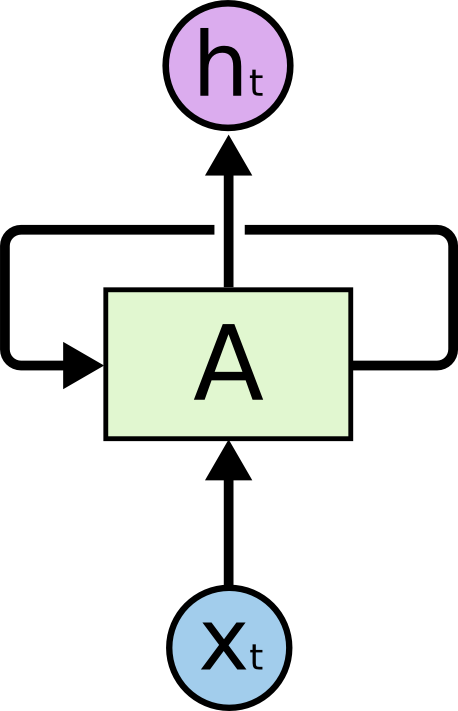
\includegraphics[width=0.2\linewidth]{Images//C5/RNN.png}
%         \vspace{0.5cm}
%         \caption{Recurrent Neural Network\\ Nguồn: https://colah.github.io, truy cập vào ngày 01/05/2025}
%     \end{figure}
%     Hình vẽ trên mô tả một đoạn của mạng nơ-ron hồi quy \textit{A} với đầu vào là $x_t$ và đầu ra là $h_t$ . Một vòng lặp cho phép thông tin có thể được truyền từ bước này qua bước này qua bước khác của mạng nơ-ron.\\
%     RNN cho phép duy trì một trạng thái ẩn (hidden state) được cập nhật liên tục theo thời gian, giúp lưu trữ thông tin từ các bước trước và sử dụng nó để xử lý bước hiện tại. Cụ thể, tại mỗi bước thời gian, RNN sẽ:
%     \begin{itemize}[label=--]
%         \item Nhận đầu vào hiện tại.
%         \item Kết hợp với trạng thái ẩn từ bước trước đó.
%         \item Tính toán trạng thái ẩn mới và đầu ra tương ứng
%     \end{itemize}
%     Nhờ cơ chế "hồi quy" này, RNN có khả năng nắm bắt mối quan hệ theo chuỗi và lưu trữ ngữ cảnh tạm thời, làm cho nó phù hợp với các bài toán thời gian thực hoặc dữ liệu tuần tự.\\
%     Tuy nhiên, RNN truyền thống vẫn gặp phải những hạn chế nghiêm trọng trong việc học các mối quan hệ dài hạn (long-term dependencies) do vấn đề vanishing gradient (gradient tiêu biến) khi huấn luyện. Để giải quyết vấn đề này, các kiến trúc nâng cao như LSTM và GRU đã được phát triển.
%     \item \textbf{Mạng LSTM}\\
%     Mạng bộ nhớ dài-ngắn (Long Short Term Memory networks), thường được gọi là LSTM - là một dạng đặc biệt của RNN, nó có khả năng học được các phụ thuộc xa. LSTM được thiết kế để tránh được vấn đề phụ thuộc xa (long-term dependency). Việc nhớ thông tin trong suốt thời gian dài là đặc tính mặc định của chúng, chứ không cần phải huấn luyện nó để có thể nhớ được. 
%     \begin{figure}[H]
%         \centering
%         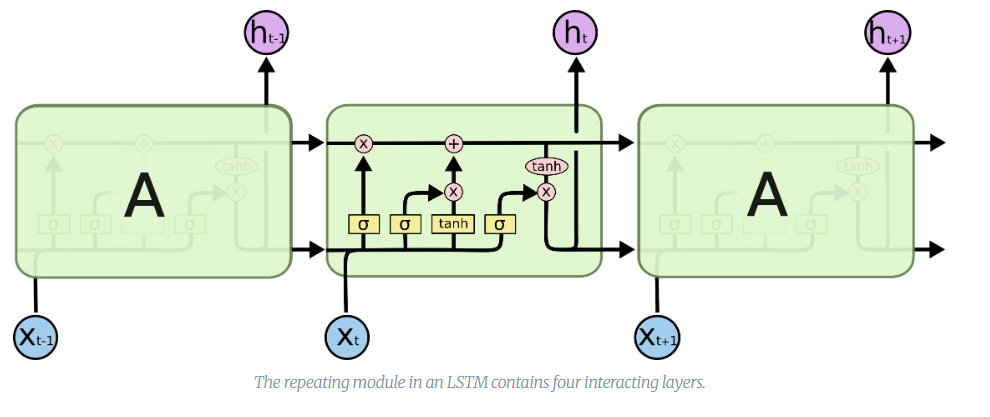
\includegraphics[width=0.75\linewidth]{Images//C5/LSTM.png}
%         \vspace{0.5cm}
%         \caption{Mạng LSTM\\ Nguồn: https://colah.github.io, truy cập vào ngày 01/05/2025}
%     \end{figure}
%     Cốt lõi của \textbf{LSTM} là \textit{cấu trúc ô nhớ (memory cell)} – nơi lưu trữ thông tin qua nhiều bước thời gian, kết hợp với ba cổng điều khiển chính (Các cổng là nơi sàng lọc thông tin đi qua nó, chúng được kết hợp bởi một tầng mạng sigmoid và một phép nhân):
%     \begin{itemize}[label=--]
%         \item Cổng vào (input gate): kiểm soát lượng thông tin mới được thêm vào ô nhớ.
%         \item Cổng quên (forget gate): quyết định thông tin nào trong ô nhớ cần được loại bỏ.
%         \item Cổng đầu ra (output gate): xác định thông tin nào sẽ được xuất ra tại bước hiện tại.
%     \end{itemize}
%     Nhờ các cơ chế này, LSTM có khả năng:
%     \begin{itemize}[label=--]
%         \item Ghi nhớ thông tin quan trọng trong thời gian dài.
%         \item Bỏ qua hoặc quên đi những thông tin không cần thiết.
%         \item Học hiệu quả các chuỗi dài mà không gặp vấn đề gradient tiêu biến như RNN.
%     \end{itemize}


% \end{enumerate}
% \subsection{Thiết kế}

% \subsubsection{Kiến trúc hệ thống}
% \noindent \textbf{Hệ thống quản lý tài sản CNTT theo thời gian thực} (Real-time IT Asset Management) được thiết kế để giám sát, quản lý và tối ưu hóa tài sản công nghệ thông tin. Kiến trúc hệ thống bao gồm nhiều thành phần chính để đảm bảo khả năng giám sát thời gian thực, lưu trữ dữ liệu hiệu quả, và hỗ trợ ra quyết định dựa trên phân tích dữ liệu. Hệ thống sẽ được thiết kế kết hợp giữa kiến trúc theo lớp.
% \begin{figure}[H]
%     \centering
%     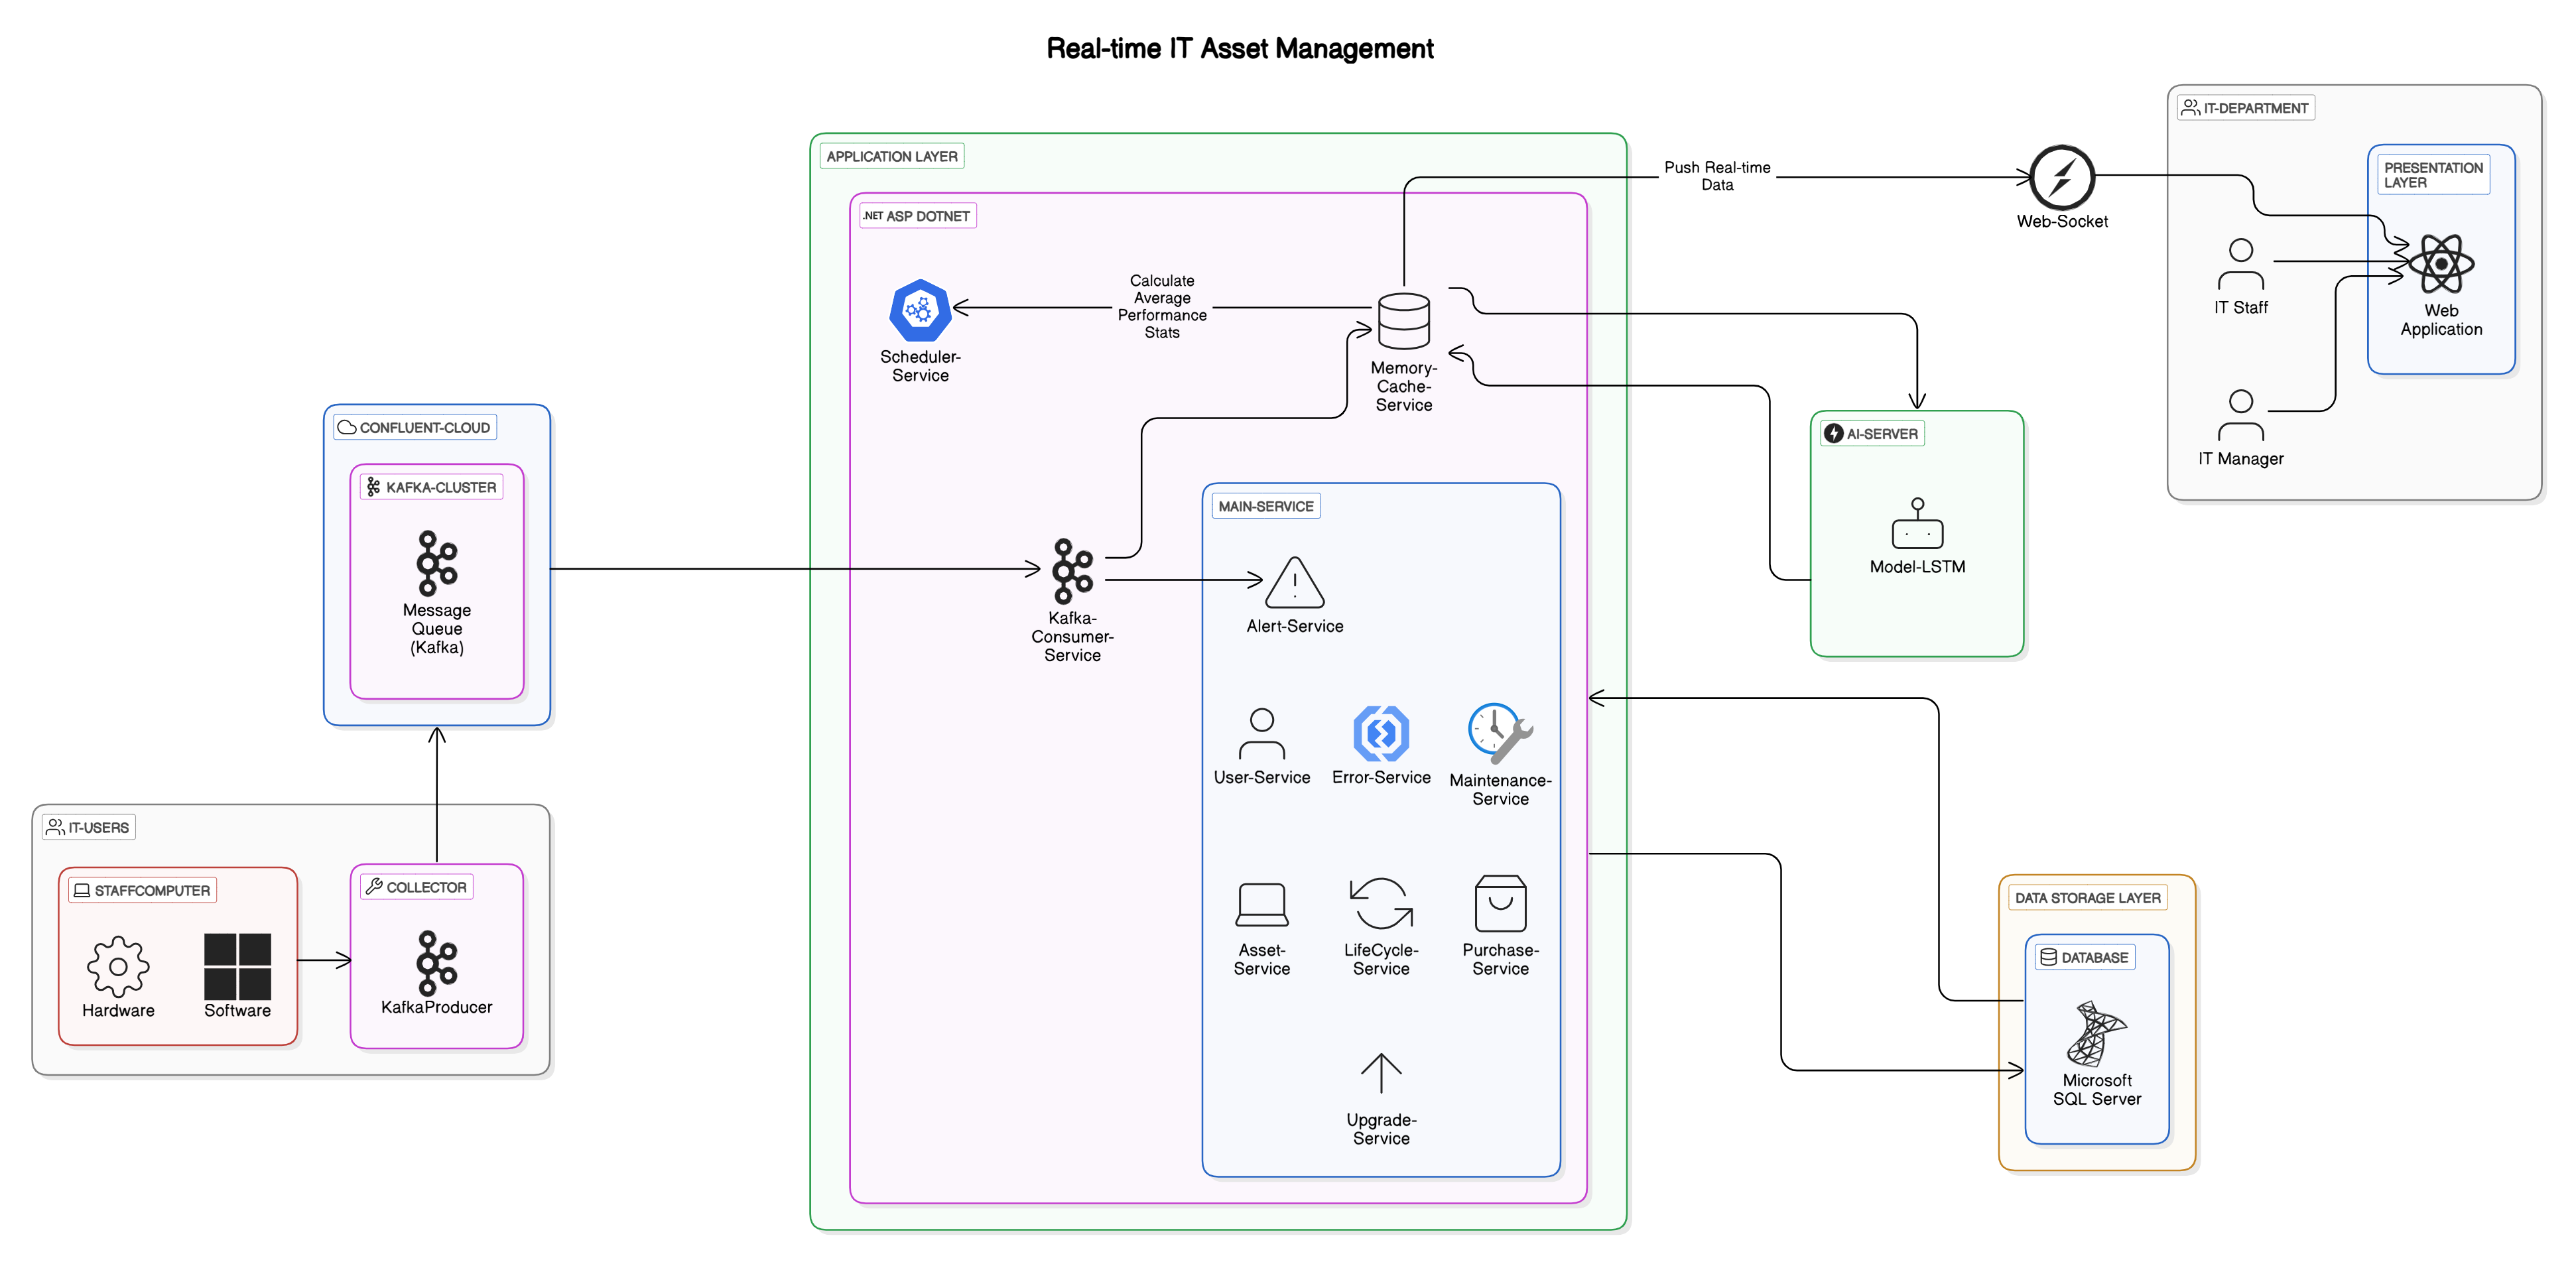
\includegraphics[width=\linewidth]{Images/C5/ITAM-Architecture.png}
%     \vspace{5pt}
%     \caption{Kiến trúc hệ thống ITAM}
% \end{figure}
% \noindent \textbf{Các thành phần chính của hệ thống}:
% \begin{enumerate}
%     \item \textbf{Bộ phận CNTT(IT Department)}:
%     \begin{itemize}[label=--]
%         \item Người dùng cuối là các nhân sự thuộc bộ phận IT, bao gồm:
%             \begin{itemize}[label=\textbullet]
%                 \item Nhân viên IT
%                 \item Quản lý
%             \end{itemize}
%         \item Cả hai đối tượng này tương tác với hệ thống qua \textbf{Presentation Layer} với Ứng dụng giao diện Web được phát triển bằng React.
%     \end{itemize}
%     \item \textbf{Tầng ứng dụng (Application Layer)}:\\
%     Tầng ứng dụng bao gồm các service:
%         \begin{itemize}[label=--]
%             \item Memory Cache Service: dùng để quản lý cache của hệ thống. Dữ liệu thời gian thực sẽ được cache lại với một khoảng thời gian nhất định.
%             \item Kafka Consumer Service: Dịch vụ chạy nền với vai trò là tiêu thụ tin nhắn từ Confluent Cloud
%             \item Scheduler Service: Dịch vụ chạy nền có vài trò là tính toán giá trị trung bình của hiệu suất mỗi ngày vào hai khung giờ là 10 giờ sáng và 14 giờ chiều.
%             \item Alert Service: dùng cho module cảnh báo
%             \item Life Cycle Service: dùng cho module quản lý vòng đời tài sản
%             \item Purchase Service: dùng cho module quản lý đơn đặt hàng
%             \item Upgrade Service: dùng để quản lý yêu cầu nâng cấp
%             \item Error \& Maintenance Service: dùng cho module quản lý sự cố và bảo trì            
%         \end{itemize}
%     \item \textbf{Tầng lưu trữ dữ liệu (Data Storage Layer) }:\\
%     Dữ liệu của hệ thống được lưu trữ trong Microsoft SQL Server, đảm bảo:
%     \begin{itemize}[label=--]
%         \item Quản lý dữ liệu liên quan đến tài sản.
%         \item Hỗ trợ lưu trữ dữ liệu về các sự kiện hệ thống.
%     \end{itemize}
%     \item \textbf{Người dùng tài sản CNTT (IT Users)}: \\
%     Tại mỗi máy của người dùng tài sản CNTT sẽ cài đặt Collector. Collector có trách nhiệm thu thập thông tin cấu hình phần cứng, phần mềm tại mỗi máy tính. Collector này đóng vai trò là Producer.
%     \item \textbf{AI Server}: Dùng để dự đoán hiệu suất tài sản
%     \item \textbf{Websocker}: Dùng để truyền dữ liệu theo thời gian thực
% \end{enumerate}
%     \textbf{Dữ liệu thu thập từ người dùng tài sản CNTT}: 
%     \begin{enumerate}
%         \item Dữ liệu từ phần cứng, phần mềm được thu thập qua Collector. \item Kafka Producer hay Collector sau đó đẩy dữ liệu lên Confluent Cloud
%         \item Dữ liệu này được Kafka Consumer Service tiêu thụ và lưu tại cache
%         \item Dữ liệu sau đó sẽ được xử lý tại các service, sau khi xử lý xong sẽ được truyền đến giao diện bằng WebSocket.
%     \end{enumerate}
% \subsubsection{Thiết kế cơ sở dữ liệu}
% \begin{figure}[H]
%     \centering
%     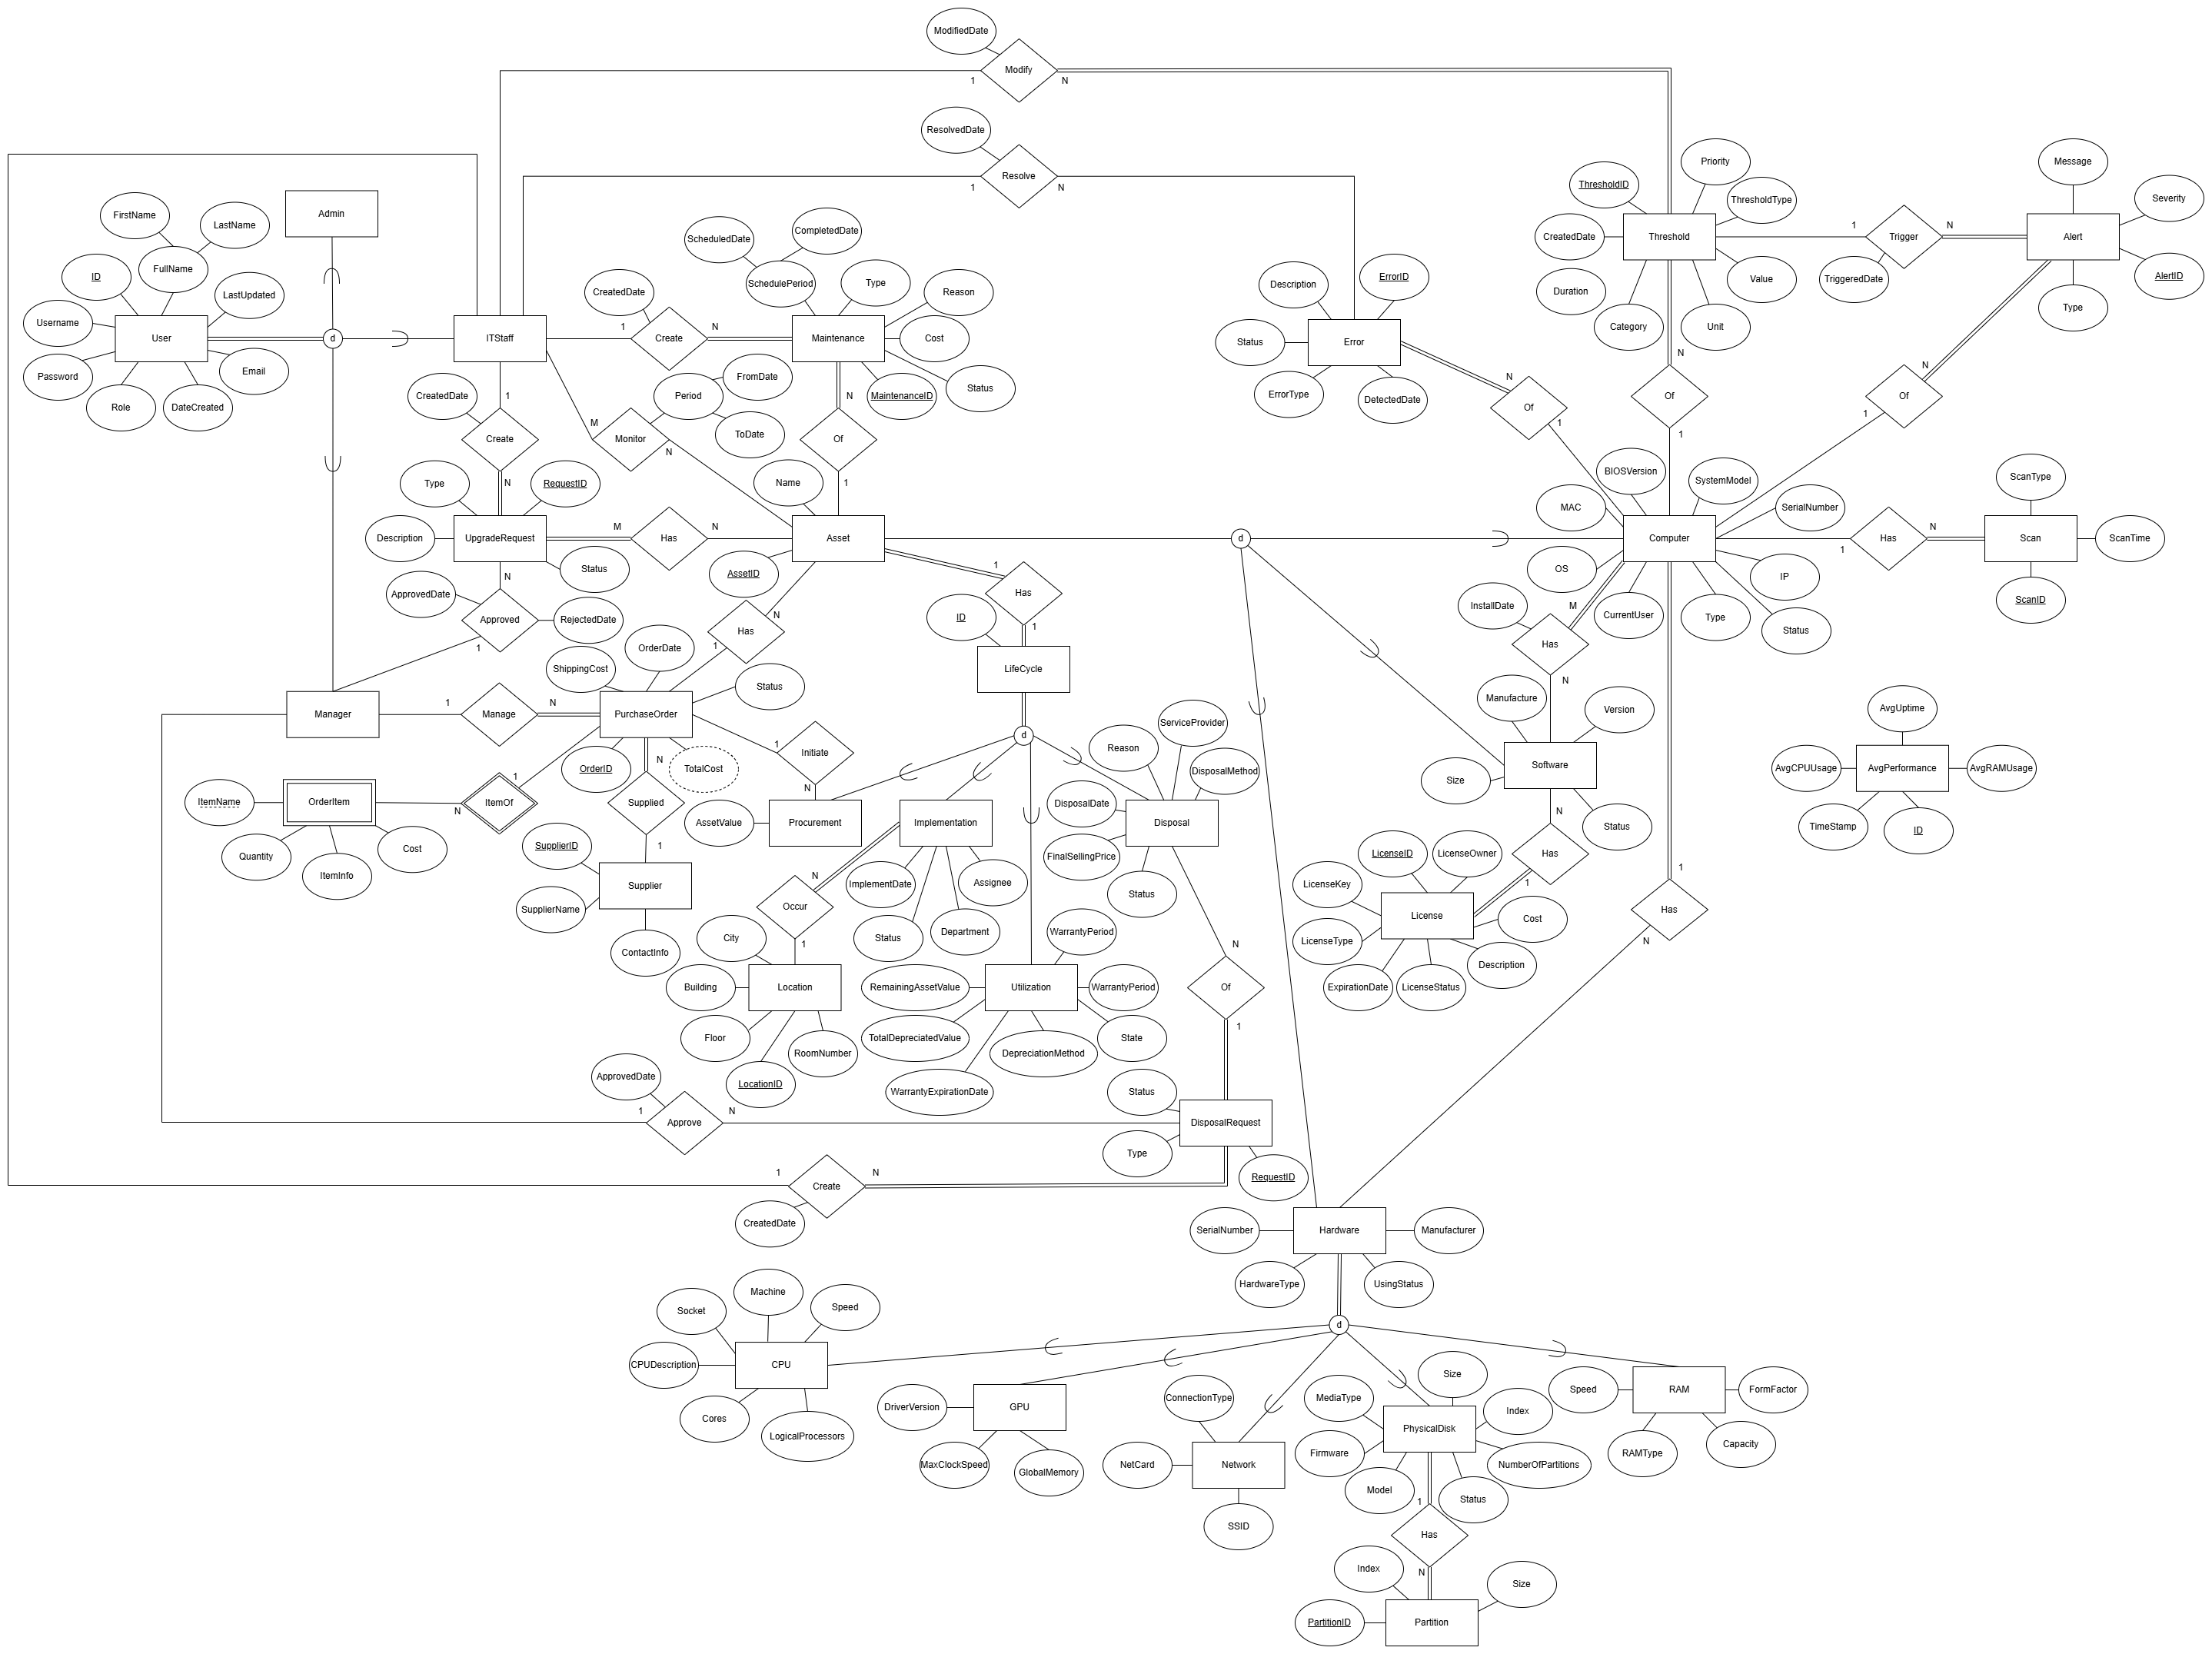
\includegraphics[width=\linewidth]{Images/C5/EERD.png}
%     \vspace{5pt}
%     \caption{Enhanced Entity-Relationship Diagram}
% \end{figure}
% \noindent \textbf{Các thành phần chính của EERD:}
% \begin{enumerate}
%     \item Thực thể (Entities)
%     \begin{itemize}[label=--]
%         \item Asset (Tài sản): Thực thể trung tâm trong hệ thống quản lý tài sản ITAM, đại diện cho mọi tài sản công nghệ thông tin trong tổ chức, bao gồm cả phần cứng, phần mềm và máy tính.
%         \item Hardware (Phần cứng): Là thực thể con của Asset, đại diện cho các tài sản vật lý thuộc về CNTT. Bao gồm nhiều thành phần phần cứng cụ thể như:
%         \begin{itemize}[label=\textbullet]
%             \item CPU: Đại diện cho bộ xử lý trung tâm của máy tính.
%             \item GPU: Đại diện cho bộ xử lý đồ họa trong hệ thống.
%             \item RAM: Đại diện cho bộ nhớ truy cập ngẫu nhiên của máy tính.
%             \item PhysicalDisk: Đại diện cho ổ đĩa vật lý được sử dụng để lưu trữ dữ liệu.
%             \item Network: Đại diện cho thiết bị mạng như card mạng và các kết nối mạng liên quan.
%         \end{itemize}
%         \item Partition (Phân vùng): Là thành phần liên quan đến PhysicalDisk, đại diện cho các phân vùng được tạo trên ổ đĩa vật lý.
%         \item Software (Phần mềm): Là thực thể con của Asset, đại diện cho các ứng dụng, phần mềm hệ thống hoặc phần mềm cài đặt trên các thiết bị.
%         \item Computer (Máy tính): Là thực thể con khác của Asset, đại diện cho các thiết bị máy tính cá nhân hoặc máy bàn, có mối quan hệ với cả các thành phần phần cứng và phần mềm được cài đặt trên máy.
%         \item License (Giấy phép): Đại diện cho các thông tin về bản quyền, thời hạn sử dụng và điều khoản liên quan đến các phần mềm thuộc tài sản.
%         \item Supplier (Nhà cung cấp): Đại diện cho các đơn vị cung cấp tài sản CNTT, phần mềm hoặc dịch vụ bảo trì liên quan.
%         \item PurchaseOrder (Đơn đặt hàng): Đại diện cho các đơn đặt hàng được tạo ra để mua sắm tài sản CNTT từ nhà cung cấp.
%         \item OrderItem (Thành phần của đơn đặt hàng): Các thành phần thông tin về tài sản cụ thể khi quản lý tạo và gửi yêu cầu đặt hàng đến với nhà cung cấp.
%         \item Threshold (Ngưỡng cảnh báo): Ghi nhận các ngưỡng cảnh báo do nhân viên cài đặt đối với từng máy tính để có thể giám sát, theo dõi và cảnh báo khi có thông số cao hoặc thấp của các tài sản liên quan đến máy tính này.
%         \item Alert (Cảnh báo): Thực thể này ghi nhận các cảnh báo liên quan đến tài sản của máy tính vượt ngưỡng cảnh báo.
%         \item Error (Lỗi): Ghi nhận các lỗi xảy ra trong quá trình thu thập dữ liệu tài sản từ collector.
%         \item  Maintenance (Bảo trì): Ghi lại các sự kiện bảo trì hoặc sửa chữa tài sản.
%         \item Upgrade Request (Yêu cầu nâng cấp): Thực thể này ghi nhận các yêu cầu nâng cấp liên quan đến một hay nhiều tài sản công nhận thông tin mà nhân viên IT sẽ đề xuất lên cho quản lý để được phê duyệt.
%         \item User (Người dùng): Thực thể cha đại diện cho các nhóm người dùng trong hệ thống.
%         \begin{itemize}[label=\textbullet]
%             \item System Administrator (Quản trị viên hệ thống): Thực thể con của User, có quyền cao nhất có toàn quyền quyết định đối với hệ thống.
%             \item IT Staff (Nhân viên IT): Quản lý và theo dõi các tài sản cụ thể, không có quyền thay đổi đơn đặt hàng.
%             \item Manager (Quản lý): Phê duyệt đơn đặt hàng và xem các báo cáo tài sản, nhưng không có quyền thay đổi cấu hình hệ thống.
%         \end{itemize}
%         \item LifeCycle (Vòng đời tài sản): Đại diện cho các giai đoạn mà một tài sản CNTT trải qua, bao gồm:
%         \begin{itemize}[label=\textbullet]
%             \item Procurement: Giai đoạn mua sắm tài sản.
%             \item Implementation: Giai đoạn cài đặt, thiết lập và triển khai sử dụng tài sản.
%             \item Utilization: Giai đoạn tài sản được đưa vào sử dụng thường xuyên trong hoạt động của tổ chức.
%             \item Disposal: Giai đoạn tài sản bị loại bỏ, thanh lý hoặc ngừng sử dụng.
%         \end{itemize}
%         \item Location (Vị trí): Đại diện cho vị trí vật lý hoặc bộ phận trong tổ chức mà tài sản được phân bổ và sử dụng.
%         \item DisposalRequest (Yêu cầu thanh lý): Ghi nhận các yêu cầu thanh lý tài sản từ nhân viên đến quản lý để thực hiện quy trình loại bỏ hợp lệ.
%         \item Scan (Quét): Đại diện cho các hoạt động quét tự động để thu thập dữ liệu tài sản từ máy tính hoặc hệ thống.
%         \item AvgPerformance (Hiệu suất trung bình): Là thực thể ghi nhận các chỉ số hiệu suất tổng hợp của tài sản, đặc biệt là máy tính, nhằm phục vụ việc giám sát và đánh giá.
%     \end{itemize}
%     \item Tổng hợp/Phân loại (Generalization/Specialization)
%     \begin{itemize}[label=--]
%         \item User (Người dùng): Là một tổng thể được phân loại thành các nhóm người dùng khác nhau, cụ thể như sau:
%         \begin{itemize}[label=\textbullet]
%             \item \textbf{Disjoint}: Một người dùng chỉ thuộc duy nhất một nhóm (không thể vừa là quản trị viên vừa là nhân viên IT).
%             \item \textbf{Total}: Mọi người dùng trong hệ thống đều phải thuộc một trong các nhóm sau: System Administrator (Quản trị viên hệ thống), IT Staff (Nhân viên IT), Manager (Quản lý).
%         \end{itemize}
%         \item Asset (Tài sản): Là thực thể tổng quát được phân loại thành ba loại tài sản cụ thể:
%         \begin{itemize}[label=\textbullet]
%             \item \textbf{Disjoint}: Mỗi tài sản chỉ thuộc duy nhất một loại (không thể vừa là phần mềm vừa là máy tính).
%             \item Total: Mọi tài sản trong hệ thống đều phải là một trong ba nhóm sau:Hardware (Phần cứng), Software (Phần mềm), Computer (Máy tính).
%         \end{itemize}
%         \item Hardware (Phần cứng): Là thực thể con của Asset, được phân loại thêm thành các thành phần phần cứng cụ thể:
%         \begin{itemize}[label=\textbullet]
%             \item \textbf{Disjoint}: Một phần cứng chỉ thuộc một loại duy nhất (ví dụ: một phần cứng không thể vừa là RAM vừa là GPU).
%             \item \textbf{Partial}: Không phải mọi phần cứng đều nhất thiết phải thuộc một trong các nhóm hiện tại, cho phép mở rộng thêm các loại phần cứng khác trong tương lai.
%             \item Các nhóm hiện tại bao gồm: CPU, GPU, RAM, PhysicalDisk, Network.
%         \end{itemize}
%         \item LifeCycle là một thực thể tổng quát mô tả toàn bộ vòng đời mà một tài sản CNTT phải trải qua, được phân loại thành các giai đoạn cụ thể:
%         \begin{itemize}[label=\textbullet]
%             \item \textbf{Disjoint}: Mỗi trạng thái cụ thể của vòng đời là tách biệt — một tài sản tại một thời điểm chỉ có thể nằm trong một giai đoạn vòng đời duy nhất.
%             \item \textbf{Total}: Mọi tài sản đều phải nằm trong một giai đoạn của vòng đời tại mọi thời điểm.
%             \item Các giai đoạn cụ thể bao gồm: Procurement (Mua sắm), Implementation (Triển khai), Utilization (Sử dụng), Disposal (Thanh lý).
%         \end{itemize}
%     \end{itemize}
%     \item Phân quyền (Authorization Levels) \\
%     Sự phân quyền giữa các nhóm người dùng được biểu diễn qua các mối quan hệ với các thực thể khác. Quyền hạn sẽ khác nhau tùy vào nhóm người dùng cụ thể, từ quản lý toàn bộ đến chỉ xem hoặc phê duyệt.
% \end{enumerate}
% \subsubsection{ Thiết kế chi tiết bên trong}
% \begin{figure}[H]
%     \centering
%     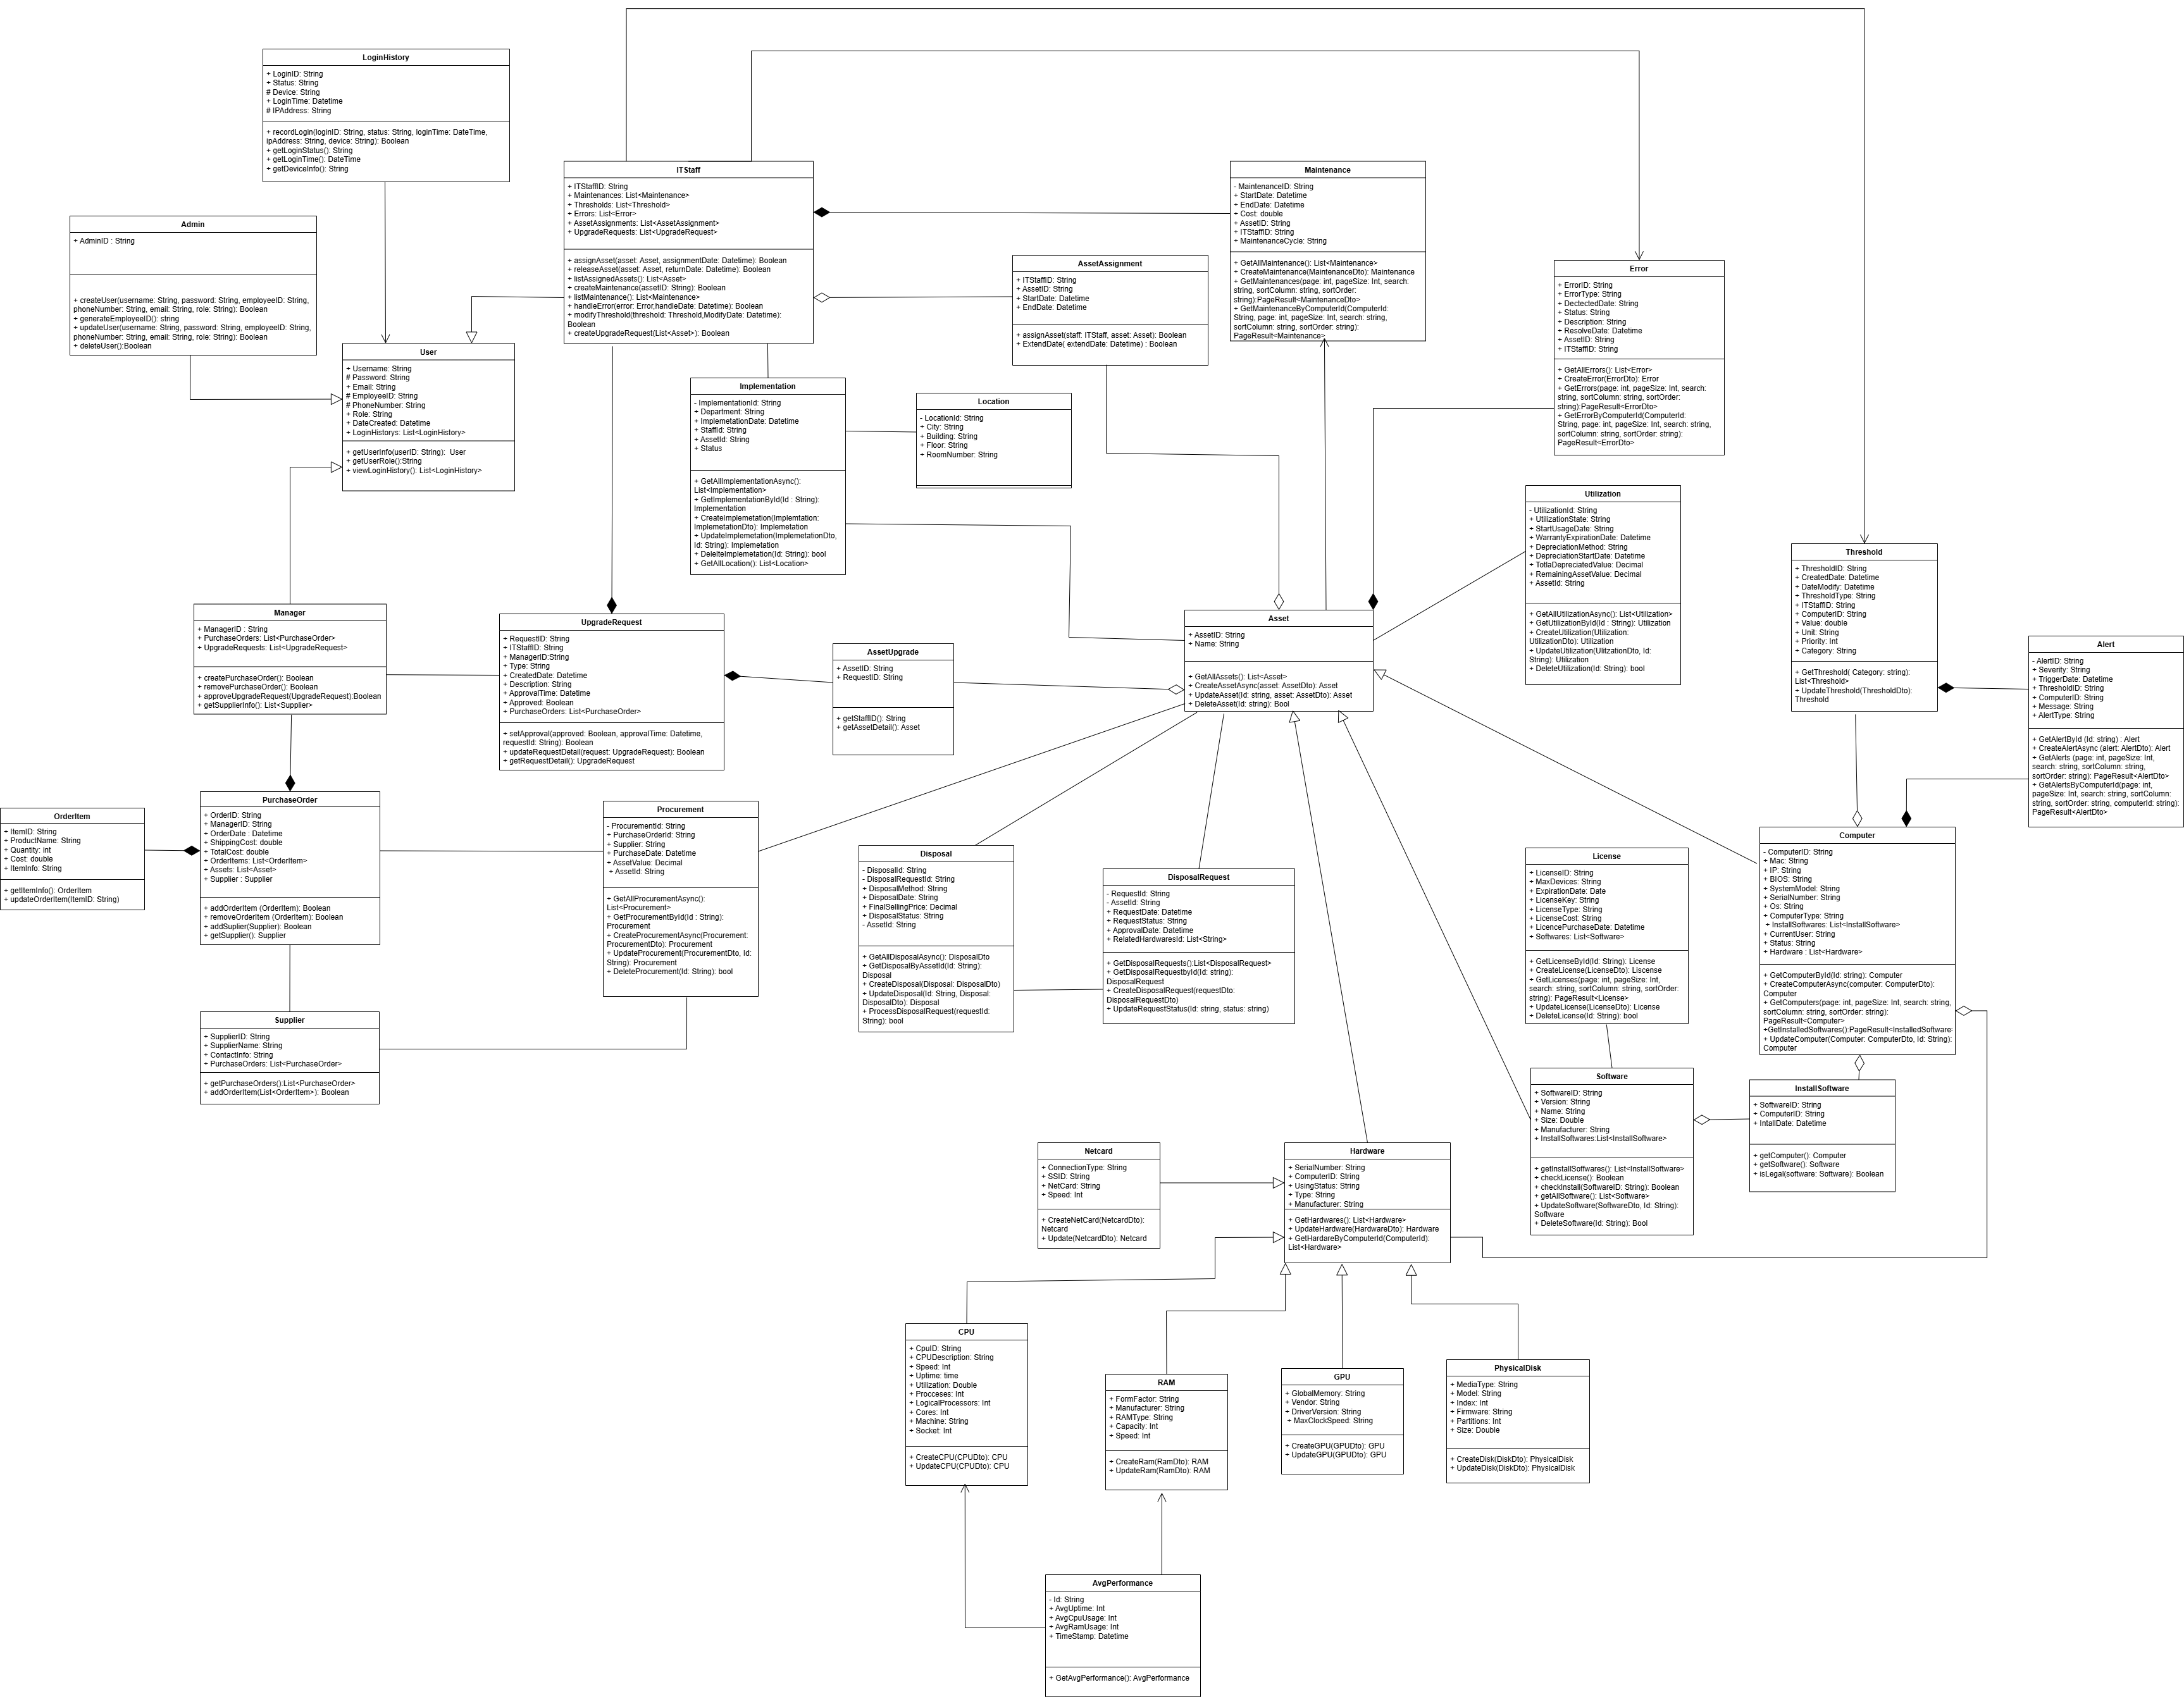
\includegraphics[width=\linewidth]{Images/C5/ClassDiagram.png}
%     \vspace{5pt}
%     \caption{Class Diagram}
% \end{figure}
% \subsection{Thiết kế API}
% \noindent Dưới đây là trình bày chi tiết thiết kế các giao diện lập trình ứng dụng (API) được sử dụng trong hệ thống. Thiết kế đầy đủ của toàn bộ hệ thống được trình bày tại đây \href{https://app.swaggerhub.com/apis/ITAMhcmut/APIDesign/1.0.0}{Link}.
% \subsubsection{Quản lý người dùng}
%     \begin{enumerate}
%         \item \textbf{Đăng nhập}
%         \begin{itemize}[label=--]
%             \item \textbf{URL:} \texttt{/api/login}
%             \item \textbf{Method:} POST
%             \item \textbf{Description:} API dùng để xác thực thông tin đăng nhập của người dùng.            
%             \item \textbf{Authorization:}
%             \begin{itemize}[label=\textbullet]
%                 \item Yêu cầu: Không yêu cầu
%                 \item Quyền truy cập: Mọi người dùng đều có thể gọi API này để đăng nhập.
%             \end{itemize}
%             \item \textbf{Request:} 
%             \begin{itemize}[label=\textbullet]
%                 \item Content-Type: \texttt{application/json}
%                 \item Request Body:
%             \end{itemize}
%             \begin{longtable}{|l|l|l|l|}
%             \hline
%             \textbf{Trường} & \textbf{Kiểu} & \textbf{Mô tả} & \textbf{Bắt buộc} \\
%             \hline
%             \endhead
%             \texttt{email} & String & Địa chỉ email người dùng & Có \\
%             \texttt{password} & String & Mật khẩu đăng nhập & Có \\
%             \hline
%             \end{longtable}
%             \item \textbf{Responses:}
%             \begin{itemize}[label=\textbullet]
%                 \item \textbf{200 OK:} Đăng nhập thành công. Dữ liệu JSON trả về:
%                 \begin{longtable}{|l|l|l|}
%                 \hline
%                 \textbf{Trường} & \textbf{Kiểu} & \textbf{Mô tả} \\
%                 \hline
%                 \endhead
%                 \texttt{accessToken} & String & Token JWT dùng để xác thực truy cập \\
%                 \hline
%                 \texttt{refreshToken} & String & Token để làm mới \texttt{accessToken}\\
%                 \hline
%                 \end{longtable}
%                 \item \textbf{500 Internal Server Error:} Có lỗi xảy ra trong quá trình xử lý hoặc người dùng không được phép đăng nhập. Không có dữ liệu trả về.
%             \end{itemize}
%         \end{itemize}
%         \item \textbf{Truy vấn thông tin của người dùng}
%         \begin{itemize}[label=--]
%             \item \textbf{URL:} \texttt{/api/users/\{id\}}
%             \item \textbf{Method:} GET
%             \item \textbf{Description:} Lấy thông tin chi tiết của người dùng cụ thể dựa trên \texttt{id}.            
%             \item \textbf{Authorization:}
%             \begin{itemize}[label=\textbullet]
%                 \item Yêu cầu: Header Authorization: Bearer <\texttt{accessToken}>
%                 \item Quyền truy cập: Administrator, Manager
%                 \item Phản hồi nếu không đủ quyền: 403 Forbidden
%             \end{itemize}
%             \item \textbf{Parameters:}
%             \begin{longtable}{|l|l|l|l|l|}
%             \hline
%             \textbf{Tên tham số} & \textbf{Vị trí} & \textbf{Kiểu dữ liệu} & \textbf{Bắt buộc} & \textbf{Mô tả} \\
%             \hline
%             \endhead
%             \texttt{id} & Path & String & Có & ID của người dùng\\
%             \hline
%             \end{longtable}
%             \item \textbf{Responses:}
%             \begin{itemize}[label=\textbullet]
%                 \item \textbf{200 OK:} Lấy thông tin thành công. Trả về dữ liệu chi tiết của người dùng.
%                 \begin{longtable}{|l|l|l|}
%                 \hline
%                 \textbf{Trường} & \textbf{Kiểu} & \textbf{Mô tả} \\
%                 \hline
%                 \endhead
%                 \texttt{id} & String & ID của người dùng \\
%                 \texttt{firstName} & String & Họ của người dùng \\
%                 \texttt{lastName} & String & Tên của người dùng \\
%                 \texttt{role} & String & Vai trò của người dùng \\
%                 \texttt{phoneNumber} & String & Số điện thoại người dùng \\
%                 \texttt{createdAt} & String & Ngày tạo tài khoản (ISO format) \\
%                 \texttt{lastUpdatedAt} & String & Ngày cập nhật gần nhất \\
%                 \texttt{accessToken} & String & Token xác thực truy cập \\
%                 \texttt{refreshToken} & String & Token làm mới \\                
%                 \hline
%                 \end{longtable}
%                 \item \textbf{403 Forbidden:} Người dùng không có quyền truy cập tài nguyên này. Không có dữ liệu trả về.
%                 \item \textbf{500 Internal Server Error} - Có lỗi xảy ra trong quá trình truy vấn người dùng. Không có dữ liệu trả về 
%             \end{itemize}
%         \end{itemize}
%     \end{enumerate}
% \subsubsection{Quản lý tài sản}
%     \begin{enumerate}
%         \item \textbf{Tạo mới máy tính}
%         \begin{itemize}[label=--]
%             \item \textbf{URL:} \texttt{/api/computer/CreateComputer}
%             \item \textbf{Method:} POST
%             \item \textbf{Description:} Tạo mới một tài sản máy tính
%             \item \textbf{Authorization:}
%             \begin{itemize}[label=\textbullet]
%                 \item Yêu cầu: Authorization: Bearer <\texttt{accessToken}>
%                 \item Quyền truy cập: Administrator, ITStaff
%                 \item Phản hồi nếu không đủ quyền: 403 Forbidden
%             \end{itemize}
%             \item \textbf{Request:}
%             \begin{itemize}[label=\textbullet]
%                 \item Content-Type: \texttt{application/json}
%                 \item Request Body:
%             \end{itemize}
%             \begin{longtable}{|l|l|l|l|}
%             \hline
%             \textbf{Trường} & \textbf{Kiểu} & \textbf{Mô tả} & \textbf{Bắt buộc} \\
%             \hline
%             \endhead
%             \texttt{name} & String & Tên thiết bị (do người dùng đặt) & Có \\
%             \texttt{model} & String & Model của máy tính & Không \\
%             \texttt{serialNumber} & String & Số serial & Không \\
%             \texttt{os} & String & Hệ điều hành & Không \\
%             \texttt{computerType} & String & Loại máy tính (Laptop, Desktop) & Có \\
%             \hline
%             \end{longtable}
%             \item \textbf{Responses:}
%             \begin{itemize}[label=\textbullet]
%                 \item \textbf{200 OK:} Tạo thành công. Trả về thông tin chi tiết của máy tính vừa được tạo. 
%                 \begin{longtable}{|l|l|l|}
%                 \hline
%                 \textbf{Trường} & \textbf{Kiểu} & \textbf{Mô tả} \\
%                 \hline
%                 \endhead
%                 \texttt{assetId} & String & Mã định danh của thiết bị \\
%                 \texttt{name} & String & Tên thiết bị \\
%                 \texttt{mac} & String & Địa chỉ MAC \\
%                 \texttt{ip} & String & Địa chỉ IP \\
%                 \texttt{bios} & String & Thông tin BIOS \\
%                 \texttt{model} & String & Model thiết bị \\
%                 \texttt{serialNumber} & String & Số serial \\
%                 \texttt{os} & String & Hệ điều hành \\
%                 \texttt{computerType} & String & Loại máy tính \\
%                 \texttt{currentUser} & String & Người dùng hiện tại \\
%                 \texttt{status} & String & Trạng thái thiết bị \\
%                 \texttt{hardware} & Array[Object] & Thông tin phần cứng chi tiết \\
%                 \hline
%                 \end{longtable}
%                 \item \textbf{403 Forbidden:} Người dùng không có quyền tạo máy tính. Không có dữ liệu trả về.
%                 \item \textbf{500 Internal Server Error:} Dữ liệu đầu vào không hợp lệ hoặc có lỗi trong quá trình xử lý. Không có dữ liệu trả về.
%             \end{itemize}
%         \end{itemize}
%         \item \textbf{Truy vấn thông tin phần cứng}
%         \begin{itemize}[label=--]
%             \item \textbf{URL:} \texttt{/api/hardware/GetHardwares}
%             \item \textbf{Method:} GET
%             \item \textbf{Description:} API này dùng để truy vấn danh sách phần cứng từ hệ thống, hỗ trợ phân trang, tìm kiếm và sắp xếp.
%             \item \textbf{Authorization:}
%             \begin{itemize}[label=\textbullet]
%                 \item Yêu cầu: Header Authorization: Bearer <\texttt{accessToken}>.
%                 \item Quyền truy cập: Administrator, Manager, ITStaff.
%                 \item Phản hồi nếu không đủ quyền: 403 Forbidden.
%             \end{itemize}
%             \item \textbf{Parameters:}
%             \begin{longtable}{|l|l|l|l|l|}
%             \hline
%             \textbf{Tên tham số} & \textbf{Vị trí} & \textbf{Kiểu} & \textbf{Bắt buộc} & \textbf{Mô tả} \\
%             \hline
%             \endhead
%             \texttt{page} & Query & Number & Không & Số trang hiện tại\\
%             \texttt{pageSize} & Query & Number & Không & Số phần tử mỗi trang \\
%             \texttt{search} & Query & String & Không & Từ khóa tìm kiếm\\
%             \texttt{sortColumn} & Query & String & Không & 	Cột dùng để sắp xếp \\
%             \texttt{sortOrder} & Query & String & Không & \texttt{asc} hoặc \texttt{desc}\\
%             \hline
%             \end{longtable}
%             \item \textbf{Responses:}
%             \begin{itemize}[label=\textbullet]
%                 \item \textbf{200 OK:} Lấy dữ liệu thành công. Trả về danh sách phần cứng và thông tin phân trang.
%                 \begin{longtable}{|l|l|l|}
%                 \hline
%                 \textbf{Trường} & \textbf{Kiểu} & \textbf{Mô tả} \\
%                 \hline
%                 \endhead
%                 \texttt{items} & Array[Object] & Danh sách phần cứng\\
%                 \texttt{totalRecords} & Number & Tổng số phần cứng trong hệ thống \\
%                 \texttt{currentPage} & Number & Trang hiện tại \\
%                 \texttt{pageSize} & Number & Số phần tử mỗi trang \\
%                 \texttt{totalPages} & Number & Tổng số trang \\
%                 \hline
%                 \end{longtable}
%                 Mỗi phần tử trong \texttt{items} sẽ là một object phần cứng, bao gồm:
%                 \begin{longtable}{|l|l|l|}
%                 \hline
%                 \textbf{Trường} & \textbf{Kiểu} & \textbf{Mô tả} \\
%                 \hline
%                 \endhead
%                 \texttt{serialNumber} & String & Số serial của phần cứng \\
%                 \texttt{computerID} & String & ID máy tính đang gắn phần cứng \\
%                 \texttt{hardwareType} & String & Loại phần cứng \\
%                 \texttt{usingStatus} & String & Trạng thái sử dụng \\
%                 \texttt{manufacturer} & String & Hãng sản xuất \\
%                 \texttt{details} & String & Thông tin chi tiết \\
%                 \texttt{assetId} & String & Mã định danh tài sản liên quan \\
%                 \texttt{name} & String & Tên định danh của phần cứng trong hệ thống \\
%                 \hline
%                 \end{longtable}
%                 \item \textbf{403 Forbidden:} Người dùng không có quyền truy cập API. Không có dữ liệu trả về.
%                 \item \textbf{500 Internal Server Error:} Dữ liệu đầu vào không hợp lệ hoặc có lỗi trong quá trình xử lý. Không có dữ liệu trả về.
%             \end{itemize}
%         \end{itemize}
%     \end{enumerate}
% \subsubsection{Yêu cầu nâng cấp tài sản}
%     \begin{enumerate}
%         \item \textbf{Tạo yêu cầu nâng cấp phần mềm}
%         \begin{itemize}[label=--]
%             \item \textbf{URL:} \texttt{/api/UpgradeRequest/software}
%             \item \textbf{Method:} POST
%             \item \textbf{Description:} API dùng để tạo mới một yêu cầu nâng cấp phần mềm cho thiết bị (tài sản).
%             \item \textbf{Authorization:}
%             \begin{itemize}[label=\textbullet]
%                 \item Yêu cầu: Header Authorization: Bearer <\texttt{accessToken}>.
%                 \item Quyền truy cập: Administrator, ITStaff.
%                 \item Phản hồi nếu không đủ quyền: 403 Forbidden.
%             \end{itemize}
%             \item \textbf{Request:}
%             \begin{itemize}[label=\textbullet]
%                 \item Content-Type: \texttt{application/json}
%                 \item Request Body:
%             \end{itemize}
%             \begin{longtable}{|l|l|l|l|}
%             \hline
%             \textbf{Trường} & \textbf{Kiểu} & \textbf{Mô tả} & \textbf{Bắt buộc} \\
%             \hline
%             \endhead
%             \texttt{description} & String & Mô tả ngắn gọn yêu cầu nâng cấp & Không \\
%             \texttt{updateReason} & String & Lý do cần nâng cấp phần mềm & Không \\
%             \texttt{assetId} & String & ID của thiết bị & Có \\
%             \texttt{updateType} & String & Loại cập nhật & Có \\
%             \texttt{managerName} & String & Tên người quản lý phê duyệt & Có \\
%             \texttt{staffName} & String & Tên nhân viên tạo yêu cầu & Có \\
%             \texttt{softwareType} & String & Loại phần mềm yêu cầu nâng cấp & Có\\
%             \texttt{softwareAlt} & String & ID của phần mềm nâng cấp & Có \\
%             \hline
%             \end{longtable}
%             \item \textbf{Responses:}
%             \begin{itemize}[label=\textbullet]
%                 \item \textbf{200 OK:} Tạo yêu cầu thành công. Trả về thông tin của yêu cầu nâng cấp vừa tạo.
%                 \begin{longtable}{|l|l|l|}
%                 \hline
%                 \textbf{Trường} & \textbf{Kiểu} & \textbf{Mô tả} \\
%                 \hline
%                 \endhead
%                 \texttt{requestId} & String & ID của yêu cầu nâng cấp \\
%                 \texttt{staffName} & String & Tên nhân viên gửi yêu cầu \\
%                 \texttt{managerName} & String & Tên người quản lý sẽ phê duyệt hoặc từ chối yêu cầu \\
%                 \texttt{createdDate} & String & Ngày tạo yêu cầu (ISO Format) \\
%                 \texttt{approvedDate} & String & Ngày yêu cầu được phê duyệt (nếu có) \\
%                 \texttt{rejectedDate} & String & Ngày yêu cầu bị từ chối (nếu có) \\
%                 \texttt{status} & String & Trạng thái hiện tại của yêu cầu \\
%                 \texttt{description} & String & Mô tả nội dung yêu cầu \\
%                 \texttt{updateReason} & String & Lý do đề xuất nâng cấp phần mềm \\
%                 \texttt{updateType} & String & Loại nâng cấp \\
%                 \texttt{typeDetail} & String & Thông tin chi tiết hơn về phần mềm cần nâng cấp \\
%                 \hline
%                 \end{longtable}
%                 \item \textbf{403 Forbidden:} Người dùng không có quyền truy cập API. Không có dữ liệu trả về.
%                 \item \textbf{500 Internal Server Error:} Dữ liệu đầu vào không hợp lệ hoặc có lỗi trong quá trình xử lý. Không có dữ liệu trả về.
%             \end{itemize}
%         \end{itemize}
%         \item \textbf{Hủy yêu cầu nâng cấp}
%         \begin{itemize}[label=--]
%             \item \textbf{URL:} \texttt{/api/UpgradeRequest/cancel/\{id\}}
%             \item \textbf{Method:} PUT
%             \item \textbf{Description:} Hủy một yêu cầu nâng cấp chưa được xử lý (trạng thái còn Pending).
%             \item \textbf{Authorization:}
%             \begin{itemize}[label=\textbullet]
%                 \item Yêu cầu: Header Authorization: Bearer <\texttt{accessToken}>.
%                 \item Quyền truy cập: Administrator, ITStaff.
%                 \item Phản hồi nếu không đủ quyền: 403 Forbidden.                
%             \end{itemize}
%             \item \textbf{Parameters:}
%             \begin{longtable}{|l|l|l|l|l|}
%             \hline
%             \textbf{Tên tham số} & \textbf{Vị trí} & \textbf{Kiểu} & \textbf{Bắt buộc} & \textbf{Mô tả} \\
%             \hline
%             \endhead
%             \texttt{id} & Path & String & Có & ID của yêu cầu cần hủy \\
%             \hline
%             \end{longtable}
%             \item \textbf{Responses:}
%             \begin{itemize}[label=\textbullet]
%                 \item \textbf{200 OK:} Hủy yêu cầu thành công. Trả về thông tin của yêu cầu đã cập nhật trạng thái.
%                 \item \textbf{403 Forbidden:} Người dùng không có quyền truy cập API. Không có dữ liệu trả về.
%                 \item \textbf{500 Internal Server Error:} Dữ liệu đầu vào không hợp lệ hoặc có lỗi trong quá trình xử lý. Không có dữ liệu trả về.
%             \end{itemize}
%         \end{itemize}
%     \end{enumerate}
% \subsubsection{Quản lý đơn đặt hàng}
%     \begin{enumerate}
%         \item \textbf{Tạo mới đơn đặt hàng}
%         \begin{itemize}[label=--]
%             \item \textbf{URL:} \texttt{/api/purchase-order/new}
%             \item \textbf{Method:} POST
%             \item \textbf{Description:} API dùng để tạo mới một đơn mua hàng với thông tin nhà cung cấp, các mặt hàng và chi phí liên quan.
%             \item \textbf{Authorization:}
%             \begin{itemize}[label=\textbullet]
%                 \item Yêu cầu: Header Authorization: Bearer <\texttt{accessToken}>.
%                 \item Quyền truy cập: Administrator, Manager
%                 \item Phản hồi nếu không đủ quyền: 403 Forbidden.
%             \end{itemize}
%             \item \textbf{Request:}
%             \begin{itemize}[label=\textbullet]
%                 \item Content-Type: \texttt{application/json}
%                 \item Request Body:
%             \end{itemize}
%             \begin{longtable}{|l|l|l|l|}
%             \hline
%             \textbf{Trường} & \textbf{Kiểu} & \textbf{Mô tả} & \textbf{Bắt buộc} \\
%             \hline
%             \endhead
%             \texttt{orderDate} & String &  Ngày tạo đơn (ISO Format) & Có  \\
%             \texttt{shippingCost} & Number & Chi phí vận chuyển & Có \\
%             \texttt{totalCost} & Number & Tổng chi phí đơn hàng & Có \\
%             \texttt{status} & String & Trạng thái đơn hàng & Có \\
%             \texttt{supplier} & Object & Thông tin nhà cung cấp & Có \\
%             \texttt{orderItems} & Array[Object] & Danh sách các mặt hàng đặt mua & Có \\
%             \hline
%             \end{longtable}
%             \item \textbf{Responses:} 
%             \begin{itemize}[label=\textbullet]
%                 \item \textbf{200 OK:} Tạo đơn hàng thành công. Trả về thông tin đơn hàng mới tạo.
%                 \item \textbf{403 Forbidden:} Người dùng không có quyền truy cập API. Không có dữ liệu trả về.
%                 \item \textbf{500 Internal Server Error:} Dữ liệu đầu vào không hợp lệ hoặc có lỗi trong quá trình xử lý. Không có dữ liệu trả về.
%             \end{itemize}
%         \end{itemize}
%     \end{enumerate}
% \subsubsection{Quản lý lỗi và bảo trì}
%     \begin{enumerate}
%         \item \textbf{Lấy danh sách lỗi theo máy tính}
%         \begin{itemize}[label=--]
%             \item \textbf{URL:} \texttt{/api/Error/computer/\{computerId\}}
%             \item \textbf{Method:} GET
%             \item \textbf{Description:} API dùng để lấy danh sách các lỗi đã được ghi nhận liên quan đến một máy tính cụ thể, hỗ trợ phân trang, tìm kiếm và sắp xếp.
%             \item \textbf{Authorization:}
%             \begin{itemize}[label=\textbullet]
%                 \item Yêu cầu: Yêu cầu: Header Authorization: Bearer <\texttt{accessToken}>.
%                 \item Quyền truy cập: Administrator, Manager, ITStaff.
%                 \item Phản hồi nếu không đủ quyền: 403 Forbidden.
%             \end{itemize}
%             \item \textbf{Parameters:}
%             \begin{longtable}{|l|l|l|l|l|}
%             \hline
%             \textbf{Tên tham số} & \textbf{Vị trí} & \textbf{Kiểu} & \textbf{Bắt buộc} & \textbf{Mô tả} \\
%             \hline
%             \endhead
%             \texttt{computerId} & Path & String & Có & ID của máy tính \\
%             \texttt{page} & Query & Number & Không & Số trang hiện tại \\
%             \texttt{pageSize} & Query & Number & Không & Số phần tử mỗi trang \\
%             \texttt{search} & Query & String & Không & Từ khóa tìm kiếm \\
%             \texttt{sortColumn} & Query & String & Không & 	Cột dùng để sắp xếp \\
%             \texttt{sortOrder} & Query & String & Không & \texttt{asc} hoặc \texttt{desc} \\
%             \hline
%             \end{longtable}
%             \item \textbf{Responses:}
%             \begin{itemize}[label=\textbullet]
%                 \item \textbf{200 OK:} Lấy dữ liệu thành công. Trả về danh sách lỗi tương ứng với máy tính và thông tin phân trang.
%                 \begin{longtable}{|l|l|l|}
%                 \hline
%                 \textbf{Trường} & \textbf{Kiểu} & \textbf{Mô tả} \\
%                 \hline
%                 \endhead
%                 \texttt{items} & Array[Object] & Danh sách lỗi\\
%                 \texttt{totalRecords} & Number & Tổng số lỗi của máy tính \\
%                 \texttt{currentPage} & Number & Trang hiện tại \\
%                 \texttt{pageSize} & Number & Số phần tử mỗi trang \\
%                 \texttt{totalPages} & Number & Tổng số trang \\
%                 \hline
%                 \end{longtable}
%                 Mỗi phần tử trong \texttt{items} sẽ là một object lỗi, bao gồm:
%                 \begin{longtable}{|l|l|l|}
%                 \hline
%                 \textbf{Trường} & \textbf{Kiểu} & \textbf{Mô tả} \\
%                 \hline
%                 \endhead
%                 \texttt{errorID} & String &  Mã lỗi \\
%                 \texttt{errorType} & String &  Loại lỗi \\
%                 \texttt{computerID} & String &  ID của máy tính xảy ra lỗi\\
%                 \texttt{computerName} & String &  Tên máy tính\\
%                 \texttt{staffName} & String & Tên nhân viên IT giám sát máy tính đó \\
%                 \texttt{status} & String & Trạng thái lỗi \\
%                 \texttt{detectedDate} & String & Ngày phát hiện lỗi (ISO Format) \\
%                 \texttt{resolvedDate} & String & Ngày khắc phục lỗi \\
%                 \texttt{description} & String & Mô tả chi tiết lỗi \\
%                 \hline
%                 \end{longtable}
%                 \item \textbf{403 Forbidden:} Người dùng không có quyền truy cập API. Không có dữ liệu trả về.
%                 \item \textbf{500 Internal Server Error:} Dữ liệu đầu vào không hợp lệ hoặc có lỗi trong quá trình xử lý. Không có dữ liệu trả về.
%             \end{itemize}
%         \end{itemize}
%         \item \textbf{Cập nhật trạng thái lỗi}
%         \begin{itemize}[label=--]
%             \item \textbf{URL:} \texttt{/api/Error/\{id\}/status}
%             \item \textbf{Method:} PATCH
%             \item \textbf{Description:} API dùng để cập nhật trạng thái của một lỗi cụ thể
%             \item \textbf{Authorization:}
%             \begin{itemize}[label=\textbullet]
%                 \item Yêu cầu: Yêu cầu: Header Authorization: Bearer <\texttt{accessToken}>.
%                 \item Quyền truy cập: Administrator, ITStaff.
%                 \item Phản hồi nếu không đủ quyền: 403 Forbidden.
%             \end{itemize}
%             \item \textbf{Parameters:}
%             \begin{longtable}{|l|l|l|l|l|}
%             \hline
%             \textbf{Tên tham số} & \textbf{Vị trí} & \textbf{Kiểu} & \textbf{Bắt buộc} & \textbf{Mô tả} \\
%             \hline
%             \endhead
%             \texttt{id} & Path & String & Có & Mã lỗi \\
%             \hline
%             \end{longtable}
%             \item \textbf{Request:}
%             \begin{itemize}[label=\textbullet]
%                 \item Content-Type: \texttt{application/json}
%                 \item Request Body:
%             \end{itemize}
%             \begin{longtable}{|l|l|l|l|}
%             \hline
%             \textbf{Trường} & \textbf{Kiểu} & \textbf{Mô tả} & \textbf{Bắt buộc} \\
%             \hline
%             \endhead
%             \texttt{newStatus} & String & Trạng thái mới của lỗi & Có  \\
%             \hline
%             \end{longtable}
%             \item \textbf{Responses:}
%             \begin{itemize}[label=\textbullet]
%                 \item \textbf{200 OK:} Cập nhật trạng thái thành công. Không có dữ liệu trả về.
%                 \item \textbf{403 Forbidden:} Người dùng không có quyền truy cập API. Không có dữ liệu trả về.
%                 \item \textbf{500 Internal Server Error:} Dữ liệu đầu vào không hợp lệ hoặc có lỗi trong quá trình xử lý. Không có dữ liệu trả về.
%             \end{itemize}
%         \end{itemize}
%         \item \textbf{Lịch sử bảo trì của tài sản}
%         \begin{itemize}[label=--]
%             \item \textbf{URL:} \texttt{/api/Maintenance/asset/\{assetId\}}
%             \item \textbf{Method:} GET
%             \item \textbf{Description:} API dùng để lấy danh sách các lần bảo trì của một tài sản cụ thể, hỗ trợ tìm kiếm, phân trang và sắp xếp.
%             \item \textbf{Authorization:}
%             \begin{itemize}[label=\textbullet]
%                 \item Yêu cầu: Yêu cầu: Header Authorization: Bearer <\texttt{accessToken}>.
%                 \item Quyền truy cập: Administrator, Manager, ITStaff.
%                 \item Phản hồi nếu không đủ quyền: 403 Forbidden.
%             \end{itemize}
%             \item \textbf{Parameters:}
%             \begin{longtable}{|l|l|l|l|l|}
%             \hline
%             \textbf{Tên tham số} & \textbf{Vị trí} & \textbf{Kiểu} & \textbf{Bắt buộc} & \textbf{Mô tả} \\
%             \hline
%             \endhead
%             \texttt{assetId} & Path & String & Có & ID của tài sản \\
%             \texttt{page} & Query & Number & Không & Số trang hiện tại \\
%             \texttt{pageSize} & Query & Number & Không & Số phần tử mỗi trang \\
%             \texttt{search} & Query & String & Không & Từ khóa tìm kiếm \\
%             \texttt{sortColumn} & Query & String & Không & 	Cột dùng để sắp xếp \\
%             \texttt{sortOrder} & Query & String & Không & \texttt{asc} hoặc \texttt{desc} \\
%             \hline
%             \end{longtable}
%             \item \textbf{Responses:}
%             \begin{itemize}[label=\textbullet]
%                 \item \textbf{200 OK:} Lấy dữ liệu thành công. Trả về danh sách bảo trì tương ứng với tài sản và thông tin phân trang.
%                 \begin{longtable}{|l|l|l|}
%                 \hline
%                 \textbf{Trường} & \textbf{Kiểu} & \textbf{Mô tả} \\
%                 \hline
%                 \endhead
%                 \texttt{items} & Array[Object] & Danh sách bảo trì\\
%                 \texttt{totalRecords} & Number & Tổng số bảo trì của tài sản \\
%                 \texttt{currentPage} & Number & Trang hiện tại \\
%                 \texttt{pageSize} & Number & Số phần tử mỗi trang \\
%                 \texttt{totalPages} & Number & Tổng số trang \\
%                 \hline
%                 \end{longtable}
%                 \item \textbf{403 Forbidden:} Người dùng không có quyền truy cập API. Không có dữ liệu trả về.
%                 \item \textbf{500 Internal Server Error:} Dữ liệu đầu vào không hợp lệ hoặc có lỗi trong quá trình xử lý. Không có dữ liệu trả về.
%             \end{itemize}
%         \end{itemize}
%     \end{enumerate}
% \subsubsection{Cài đặt ngưỡng cảnh báo}
%     \begin{enumerate}
%         \item \textbf{Thêm ngưỡng cảnh báo}
%         \begin{itemize}[label=--]
%             \item \textbf{URL:} \texttt{/api/threshold}
%             \item \textbf{Method:} POST
%             \item \textbf{Description:} API dùng để thêm mới một ngưỡng cảnh báo cho hệ thống.
%             \item \textbf{Request:} 
%             \begin{itemize}[label=\textbullet]
%                 \item Content-Type: \texttt{application/json}
%                 \item Request Body:
%             \end{itemize}
%             \begin{longtable}{|l|l|l|l|}
%             \hline
%             \textbf{Tên trường} & \textbf{Kiểu} & \textbf{Mô tả} & \textbf{Bắt buộc} \\
%             \hline
%             \endhead
%             \texttt{createdDate} & String & Ngày tạo ngưỡng cảnh báo & Có \\
%             \texttt{modifiedDate} & String & Ngày cập nhật cuối & Không \\
%             \texttt{thresholdType} & String & Loại ngưỡng & Có \\
%             \texttt{thresholdValue} & Number & Giá trị ngưỡng & Có \\
%             \texttt{duration} & Number & Thời lượng duy trì ngưỡng & Không \\
%             \texttt{unit} & String & Đơn vị ngưỡng & Có \\
%             \texttt{staffId} & String & ID của nhân viên thiết lập & Có \\
%             \hline
%             \end{longtable}
%             \item \textbf{Responses:}
%             \begin{itemize}[label=\textbullet]
%                 \item \textbf{200 OK:} Tạo mới ngưỡng cảnh báo thành công. Trả về thông tin ngưỡng mới được tạo.
%                 \item \textbf{403 Forbidden:} Người dùng không có quyền truy cập API. Không có dữ liệu trả về.
%                 \item \textbf{500 Internal Server Error:} Dữ liệu đầu vào không hợp lệ hoặc có lỗi trong quá trình xử lý. Không có dữ liệu trả về.
%             \end{itemize}
%         \end{itemize}
%         \item \textbf{Lấy danh sách cảnh báo theo máy tính}
%         \begin{itemize}[label=--]
%             \item \textbf{URL:} \texttt{/api/alert/computer/\{computerId\}}
%             \item \textbf{Method:} GET
%             \item \textbf{Description:} API dùng để lấy danh sách các cảnh báo đã được ghi nhận liên quan đến một máy tính cụ thể, hỗ trợ phân trang, tìm kiếm và sắp xếp.
%             \item \textbf{Authorization:}
%             \begin{itemize}[label=\textbullet]
%                 \item Yêu cầu: Yêu cầu: Header Authorization: Bearer <\texttt{accessToken}>.
%                 \item Quyền truy cập: Administrator, ITStaff.
%                 \item Phản hồi nếu không đủ quyền: 403 Forbidden.
%             \end{itemize}
%             \item \textbf{Parameters:}
%             \begin{longtable}{|l|l|l|l|l|}
%             \hline
%             \textbf{Tên tham số} & \textbf{Vị trí} & \textbf{Kiểu} & \textbf{Bắt buộc} & \textbf{Mô tả} \\
%             \hline
%             \endhead
%             \texttt{computerId} & Path & String & Có & ID của máy tính \\
%             \texttt{page} & Query & Number & Không & Số trang hiện tại \\
%             \texttt{pageSize} & Query & Number & Không & Số phần tử mỗi trang \\
%             \texttt{search} & Query & String & Không & Từ khóa tìm kiếm \\
%             \texttt{sortColumn} & Query & String & Không & 	Cột dùng để sắp xếp \\
%             \texttt{sortOrder} & Query & String & Không & \texttt{asc} hoặc \texttt{desc} \\
%             \hline
%             \end{longtable}
%             \item \textbf{Responses:}
%             \begin{itemize}[label=\textbullet]
%                 \item \textbf{200 OK:} Lấy dữ liệu thành công. Trả về danh sách cảnh báo tương ứng với máy tính và thông tin phân trang.
%                 \item \textbf{403 Forbidden:} Người dùng không có quyền truy cập API. Không có dữ liệu trả về.
%                 \item \textbf{500 Internal Server Error:} Dữ liệu đầu vào không hợp lệ hoặc có lỗi trong quá trình xử lý. Không có dữ liệu trả về.
%             \end{itemize}
%         \end{itemize}
%     \end{enumerate} 
% \subsubsection{Vòng đời tài sản}
%     \begin{enumerate}
%         \item \textbf{Lấy thông tin triển khai của tài sản}
%         \begin{itemize}[label=--]
%             \item \textbf{URL:} \texttt{/api/life-cycle/implementation/asset/\{assetId\}}
%             \item \textbf{Method:} GET
%             \item \textbf{Description:} Trả về thông tin triển khai (Implementation) của một tài sản cụ thể.
%             \item \textbf{Authorization:}
%             \begin{itemize}[label=\textbullet]
%                 \item Yêu cầu: Yêu cầu: Header Authorization: Bearer <\texttt{accessToken}>.
%                 \item Quyền truy cập: Administrator, Manager, ITStaff.
%                 \item Phản hồi nếu không đủ quyền: 403 Forbidden.
%             \end{itemize}
%             \item \textbf{Parameters:}
%             \begin{longtable}{|l|l|l|l|l|}
%             \hline
%             \textbf{Tên tham số} & \textbf{Vị trí} & \textbf{Kiểu} & \textbf{Bắt buộc} & \textbf{Mô tả} \\
%             \hline
%             \endhead
%             \texttt{assetId} & Path & String & Có & ID của tài sản \\
%             \hline
%             \end{longtable}
%             \item \textbf{Responses:}
%             \begin{itemize}[label=\textbullet]
%                 \item \textbf{200 OK:} Lấy dữ liệu thành công. Trả về thông tin triển khai tương ứng với tài sản.
%                 \begin{longtable}{|l|l|l|}
%                 \hline
%                 \textbf{Trường} & \textbf{Kiểu} & \textbf{Mô tả} \\
%                 \hline
%                 \endhead
%                 \texttt{implementationId} & String & Mã triển khai \\
%                 \texttt{department} & String & Phòng ban triển khai \\
%                 \texttt{implementationDate} & String & Ngày triển khai (ISO Format) \\
%                 \texttt{responsiblePerson} & String & Người phụ trách \\
%                 \texttt{status} & String & Trạng thái triển khai \\
%                 \texttt{assetId} & String & ID tài sản\\
%                 \texttt{locationId} & String & ID vị trí \\
%                 \texttt{location} & Object & Thông tin vị trí \\
%                 \hline
%                 \end{longtable}
%                 \item \textbf{403 Forbidden:} Người dùng không có quyền truy cập API. Không có dữ liệu trả về.
%                 \item \textbf{500 Internal Server Error:} Dữ liệu đầu vào không hợp lệ hoặc có lỗi trong quá trình xử lý. Không có dữ liệu trả về.
%             \end{itemize}
%         \end{itemize}
%         \item \textbf{Lấy thông tin thanh lý của tài sản}
%         \begin{itemize}[label=--]
%             \item \textbf{URL:} \texttt{/api/life-cycle/disposal/asset/\{assetId\}}
%             \item \textbf{Method:} GET
%             \item \textbf{Description:} Trả về thông tin thanh lý (Disposal) của một tài sản cụ thể.
%             \item \textbf{Authorization:}
%             \begin{itemize}[label=\textbullet]
%                 \item Yêu cầu: Yêu cầu: Header Authorization: Bearer <\texttt{accessToken}>.
%                 \item Quyền truy cập: Administrator, Manager, ITStaff.
%                 \item Phản hồi nếu không đủ quyền: 403 Forbidden.
%             \end{itemize}
%             \item \textbf{Parameters:}
%             \begin{longtable}{|l|l|l|l|l|}
%             \hline
%             \textbf{Tên tham số} & \textbf{Vị trí} & \textbf{Kiểu} & \textbf{Bắt buộc} & \textbf{Mô tả} \\
%             \hline
%             \endhead
%             \texttt{assetId} & Path & String & Có & ID của tài sản \\
%             \hline
%             \end{longtable}
%             \item \textbf{Responses:}
%             \begin{itemize}[label=\textbullet]
%                 \item \textbf{200 OK:} Lấy dữ liệu thành công. Trả về thông tin thanh lý tương ứng với tài sản.
%                 \begin{longtable}{|l|l|l|}
%                 \hline
%                 \textbf{Trường} & \textbf{Kiểu} & \textbf{Mô tả} \\
%                 \hline
%                 \endhead
%                 \texttt{disposalId} & String & Mã thanh lý \\
%                 \texttt{disposalRequestId} & String & Mã yêu cầu thanh lý\\
%                 \texttt{disposalMethod} & String & Phương thức thanh lý\\
%                 \texttt{disposalDate} & String & Ngày thanh lý \\
%                 \texttt{finalSellingPrice} & Number & Giá bán cuối cùng \\
%                 \texttt{disposalServiceProvider} & String & Đơn vị cung cấp dịch vụ \\
%                 \texttt{disposalStatus} & String & Trạng thái thanh lý \\
%                 \texttt{disposalReason} & String & Lý do thanh lý \\
%                 \texttt{assetId} & String & ID tài sản \\
%                 \hline
%                 \end{longtable}
%                 \item \textbf{403 Forbidden:} Người dùng không có quyền truy cập API. Không có dữ liệu trả về.
%                 \item \textbf{500 Internal Server Error:} Dữ liệu đầu vào không hợp lệ hoặc có lỗi trong quá trình xử lý. Không có dữ liệu trả về.
%             \end{itemize}
%         \end{itemize}
%     \end{enumerate}
% \subsubsection{Dự đoán hiệu suất tài sản}

%      \begin{itemize}[label=--]
%             \item \textbf{URL:} \texttt{/api/performance/predictasset/\{assetId\}}
%             % \item \textbf{URL:} \texttt{/api/life-cycle/disposal/asset/\{assetId\}}
%             \item \textbf{Method:} GET
%             \item \textbf{Description:} Dữ liệu dự đoán hiệu suất tài sản
%             \item \textbf{Authorization:}
%             \begin{itemize}[label=\textbullet]
%                 \item Yêu cầu: Yêu cầu: Header Authorization: Bearer <\texttt{accessToken}>.
%                 \item Quyền truy cập: Administrator, Manager, ITStaff.
%                 \item Phản hồi nếu không đủ quyền: 403 Forbidden.
%             \end{itemize}
%             \item \textbf{Parameters:}
%             \begin{longtable}{|l|l|l|l|l|}
%             \hline
%             \textbf{Tên tham số} & \textbf{Vị trí} & \textbf{Kiểu} & \textbf{Bắt buộc} & \textbf{Mô tả} \\
%             \hline
%             \endhead
%             \texttt{assetId} & Path & String & Có & ID của tài sản \\
%             \hline
%             \end{longtable}
%             \item \textbf{Responses:}
%             \begin{itemize}[label=\textbullet]
%                 \item \textbf{200 OK:} Lấy dữ liệu thành công. Trả về thông tin dự đoán hiệu suất tài sản.
%                 \begin{longtable}{|l|l|l|}
%                 \hline
%                 \textbf{Trường} & \textbf{Kiểu} & \textbf{Mô tả} \\
%                 \hline
%                 \endhead
%                 \texttt{ActualCpu} & List & Hiệu suất thực CPU trong 1 tiếng trước \\
%                 \texttt{ActualRam} & List & Hiệu suất thực Ram trong 1 tiếng trước\\
%                 \texttt{PredictedRam} & List & Hiệu suất Ram dự đoán\\
%                 \texttt{PredictedCpu} & List & Hiệu suất Cpu dự đoán \\
%                 \texttt{CpuMessage} & String & Cảnh báo sớm cho Cpu \\
%                 \texttt{RamMessage} & String & Cảnh báo sớm cho Ram \\
%                 \hline
%                 \end{longtable}
%                 \item \textbf{403 Forbidden:} Người dùng không có quyền truy cập API. Không có dữ liệu trả về.
%                 \item \textbf{500 Internal Server Error:} Dữ liệu đầu vào không hợp lệ hoặc có lỗi trong quá trình xử lý. Không có dữ liệu trả về.
%             \end{itemize}
%         \end{itemize}
% \subsection{Kết chương}
% \noindent Trong chương này, nhóm đã thực hiện các bước phân tích và thiết kế hệ thống với mục tiêu xây dựng một giải pháp Quản lý tài sản CNTT thời gian thực. Quá trình phát triển được chia thành ba phần chính: \textbf{phân tích, giải pháp công nghệ, và thiết kế hệ thống}.\\ \\
% \noindent Ở phần \textbf{phân tích}, nhóm đã mô hình hóa chi tiết các quy trình nghiệp vụ cốt lõi như: giám sát tài sản, quản lý vòng đời tài sản, cảnh báo sự cố và quản lý đơn đặt hàng. Các luồng thực thi được thể hiện thông qua hệ thống các use case cụ thể, giúp đảm bảo hệ thống đáp ứng đầy đủ yêu cầu của người dùng trong thực tế.\\ \\
% \noindent Tiếp theo, ở phần \textbf{giải pháp công nghệ}, nhóm đã tập trung phân tích khả năng thu thập và xử lý dữ liệu thời gian thực – một trong những yêu cầu then chốt của hệ thống. \textbf{Công nghệ Apache Kafka} trên nền tảng \textbf{Confluent Cloud} đã được lựa chọn làm giải pháp chính cho việc truyền tải dữ liệu hiệu suất từ các máy người dùng về hệ thống. Nhóm cũng đã phân tích và so sánh Kafka với các công nghệ thu thập dữ liệu thời gian thực khác để làm rõ lý do cho lựa chọn này.\\ \\
% \noindent Đặc biệt, nhóm đã tích hợp thêm thành phần AI Server sử dụng mô hình LSTM nhằm dự đoán hiệu suất hoạt động của tài sản CNTT theo thời gian. Việc ứng dụng mô hình LSTM không chỉ giúp đưa ra cảnh báo sớm mà còn góp phần nâng cao hiệu quả vận hành và giảm thiểu rủi ro trong quản lý thiết bị.\\ \\
% \noindent Trong phần \textbf{thiết kế}, nhóm đã hoàn thiện kiến trúc hệ thống gồm ba lớp: Presentation Layer, Application Layer và Data Storage Layer. Kiến trúc mới này được mô tả rõ trong sơ đồ kiến trúc tổng thể. Công nghệ React được sử dụng cho giao diện người dùng, ASP.NET Core đảm nhiệm backend, và Microsoft SQL Server là hệ quản trị cơ sở dữ liệu chính. Nhóm cũng đã thiết kế ERD để xác định mối quan hệ giữa các thực thể dữ liệu, sử dụng class diagram để mô tả chi tiết bên trong hệ thống.\\ \\
% \noindent Thiết kế API cung cấp một cấu trúc rõ ràng và đầy đủ, đảm bảo khả năng tương tác giữa các thành phần trong hệ thống. Các endpoint được tổ chức theo từng module chức năng như giám sát tài sản, quản lý vòng đời tài sản, quản lý dữ liệu phần cứng phần mềm, cảnh báo và quản lý đơn đặt hàng. Mỗi API đều được mô tả chỉ tiết về phương thức HTTP, định dạng dữ liệu yêu cầu và phản hồi, cùng với các kịch bản lỗi phổ biến. Điều này giúp đảm bảo tính thống nhất và dễ dàng trong việc triển khai hệ thống. \\ \\
% \noindent Tổng thể, chương này đã đóng vai trò nền tảng để xây dựng một hệ thống hoàn chỉnh, đảm bảo khả năng mở rộng, hiệu suất và khả năng thích ứng với nhu cầu thực tế.
% % \subsubsection{ Thiết kế giao diện}
% % \begin{itemize}

% \item{Đăng nhập}
% \begin{figure}[H]
%     \centering
%     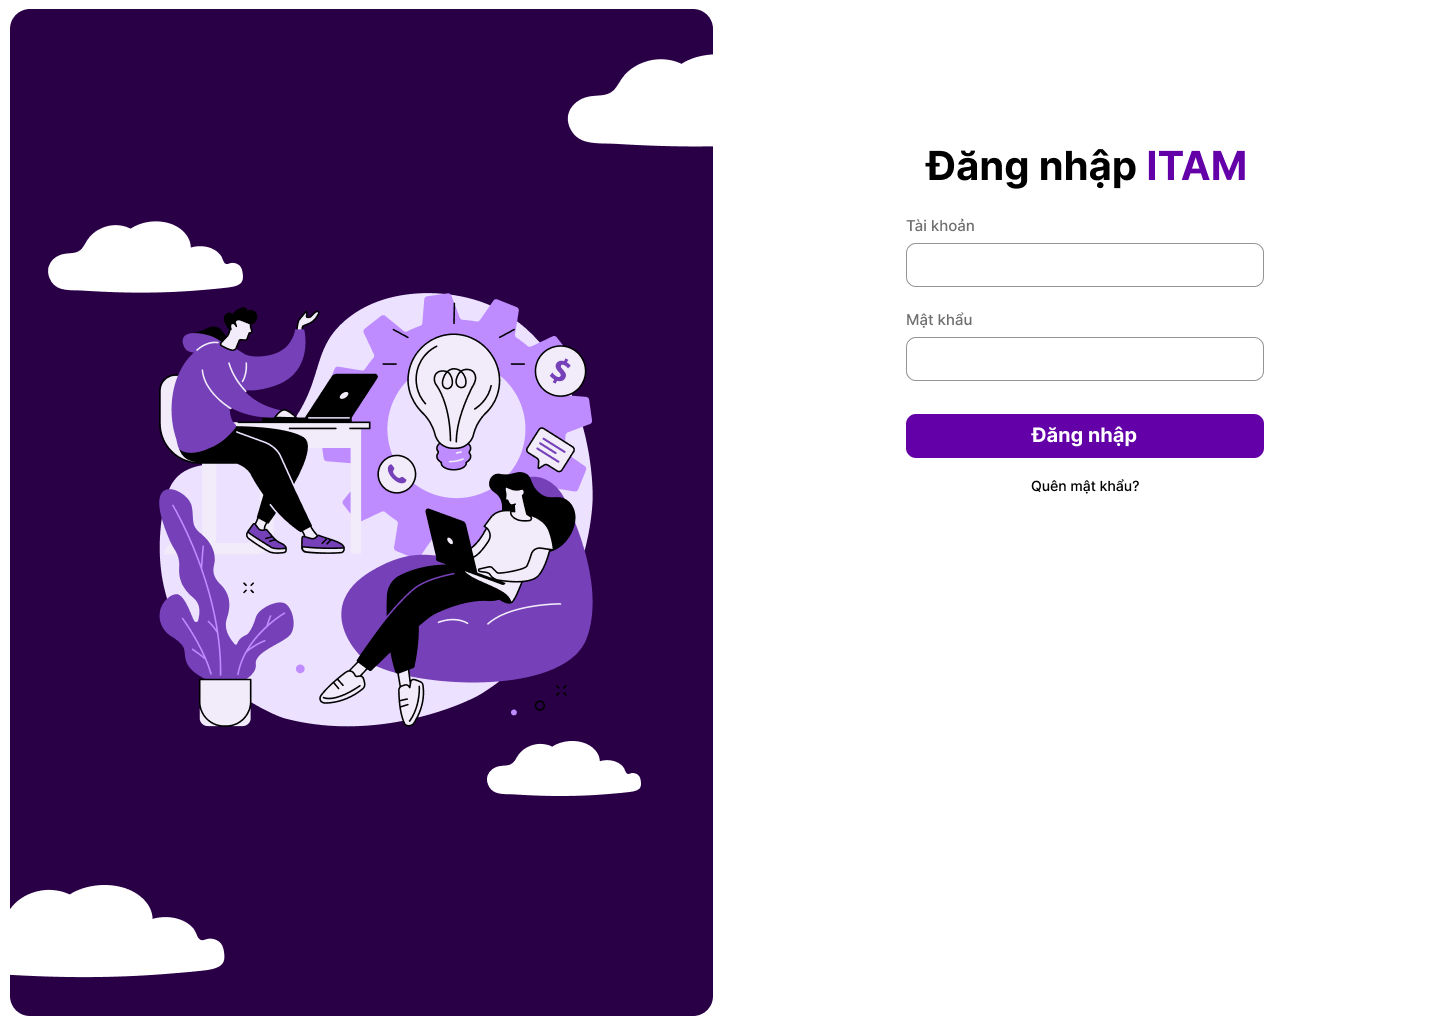
\includegraphics[width=14cm]{Images/C5/UI/Login.png}
%     \vspace{15pt}
%     \caption{Giao diện Đăng nhập}
% \end{figure}

\item{Bảng giám sát}\\
Bảng giám sát thời gian thực hiển thị trạng thái của máy tính có trong hệ thống, giúp nhân viên IT dễ dàng thực hiện giám sát máy tính, xử lý sự cố và cảnh báo một cách kịp thời, đảm bảo hoạt động của các máy tính trong hệ thống. Ngoài ra, tính năng xem tổng quan hoạt động của máy tính trong hệ thống giúp người dùng có cái nhìn tổng quan về hoạt động của các máy tính, cung cấp các thống kê về sự cố và tình trạng máy tính.
\begin{figure}[H]
    \centering
    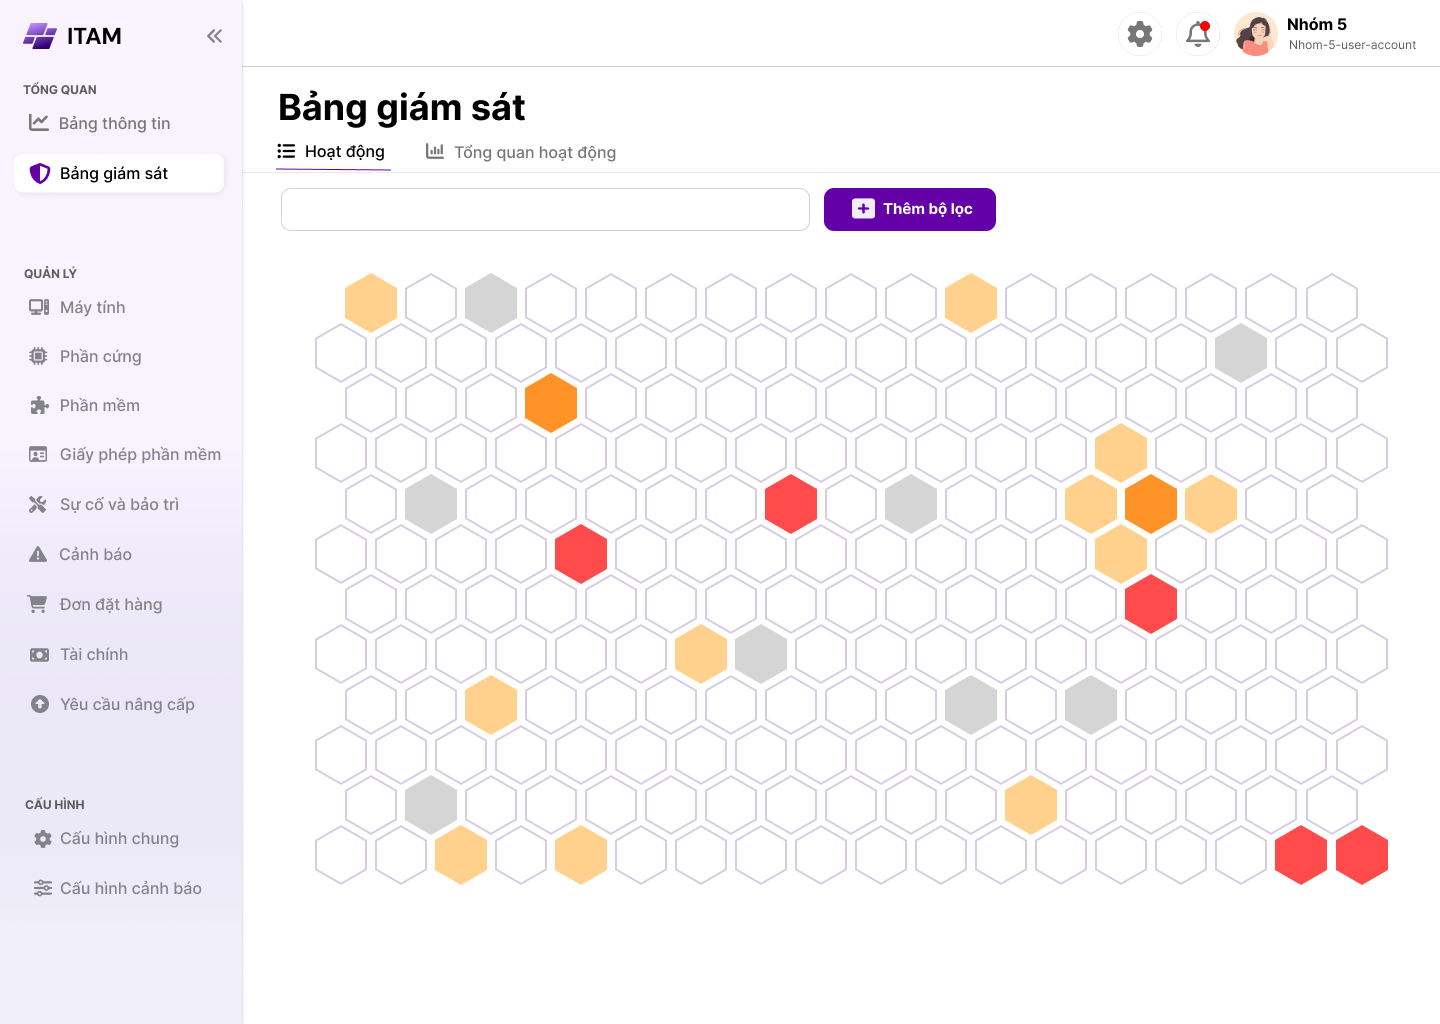
\includegraphics[width=14cm]{Images/C5/UI/Feature-Bảng giám sát 1.1.png}
    \vspace{15pt}
    \caption{Giao diện Bảng giám sát 1}
\end{figure}
% \begin{figure}[H]
%     \centering
%     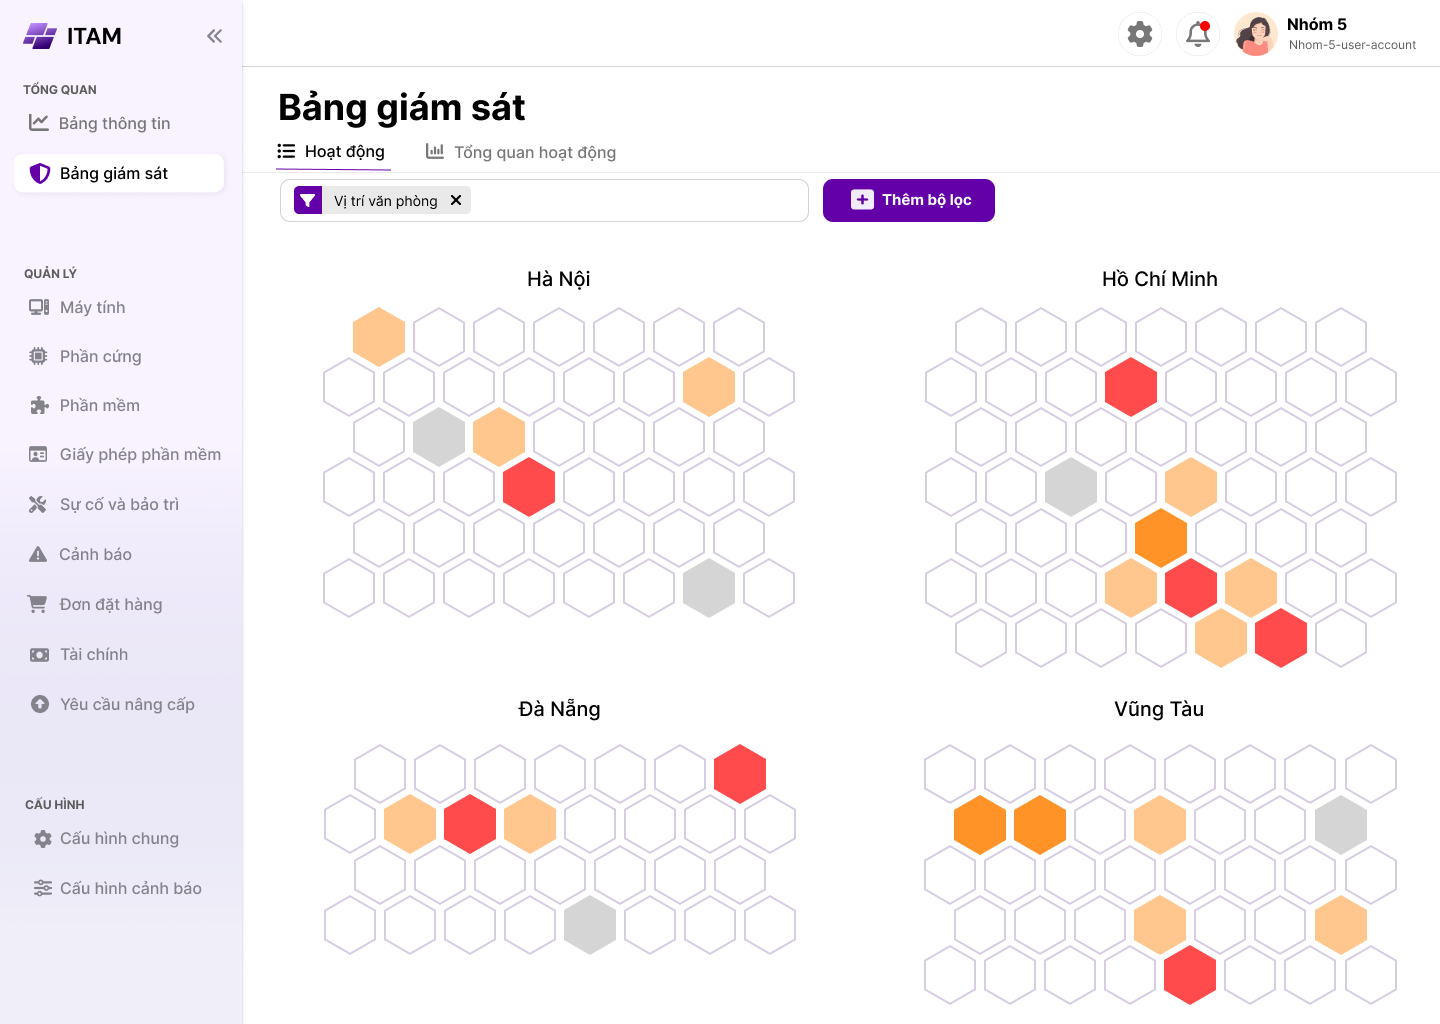
\includegraphics[width=14cm]{Images/C5/UI/Feature-Bảng giám sát 1.2.png}
%     \vspace{15pt}
%     \caption{Giao diện Bảng giám sát 2}
% \end{figure}
% \begin{figure}[H]
%     \centering
%     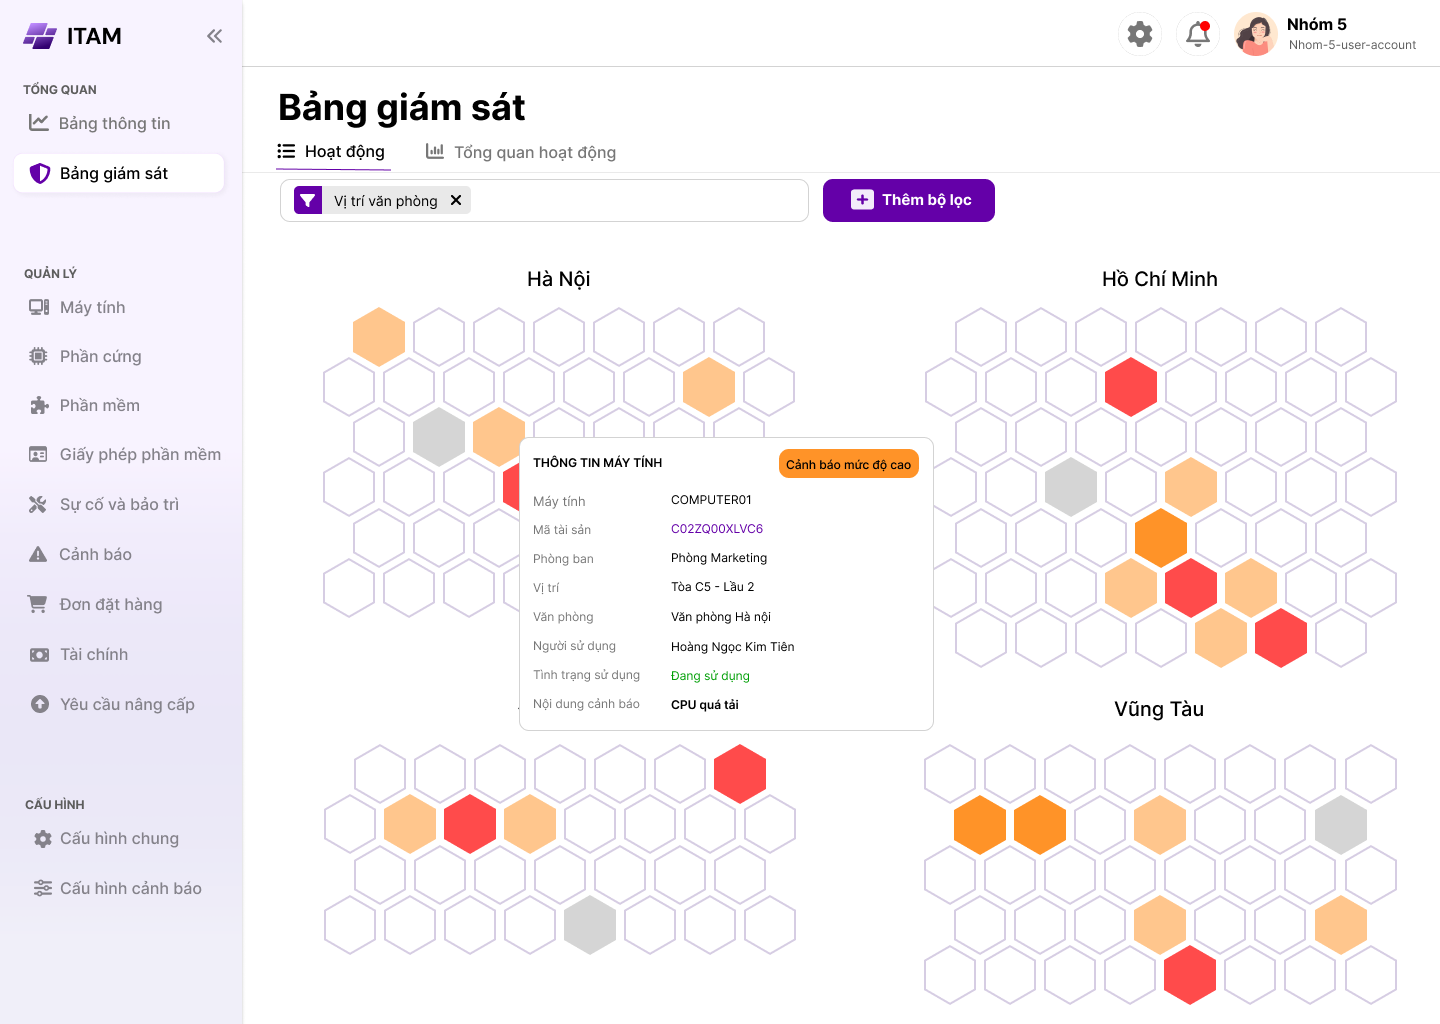
\includegraphics[width=14cm]{Images/C5/UI/Feature-Bảng giám sát 1.3.png}
%     \vspace{15pt}
%     \caption{Giao diện Bảng giám sát 2}
% \end{figure}
% \begin{figure}[H]
%     \centering
%     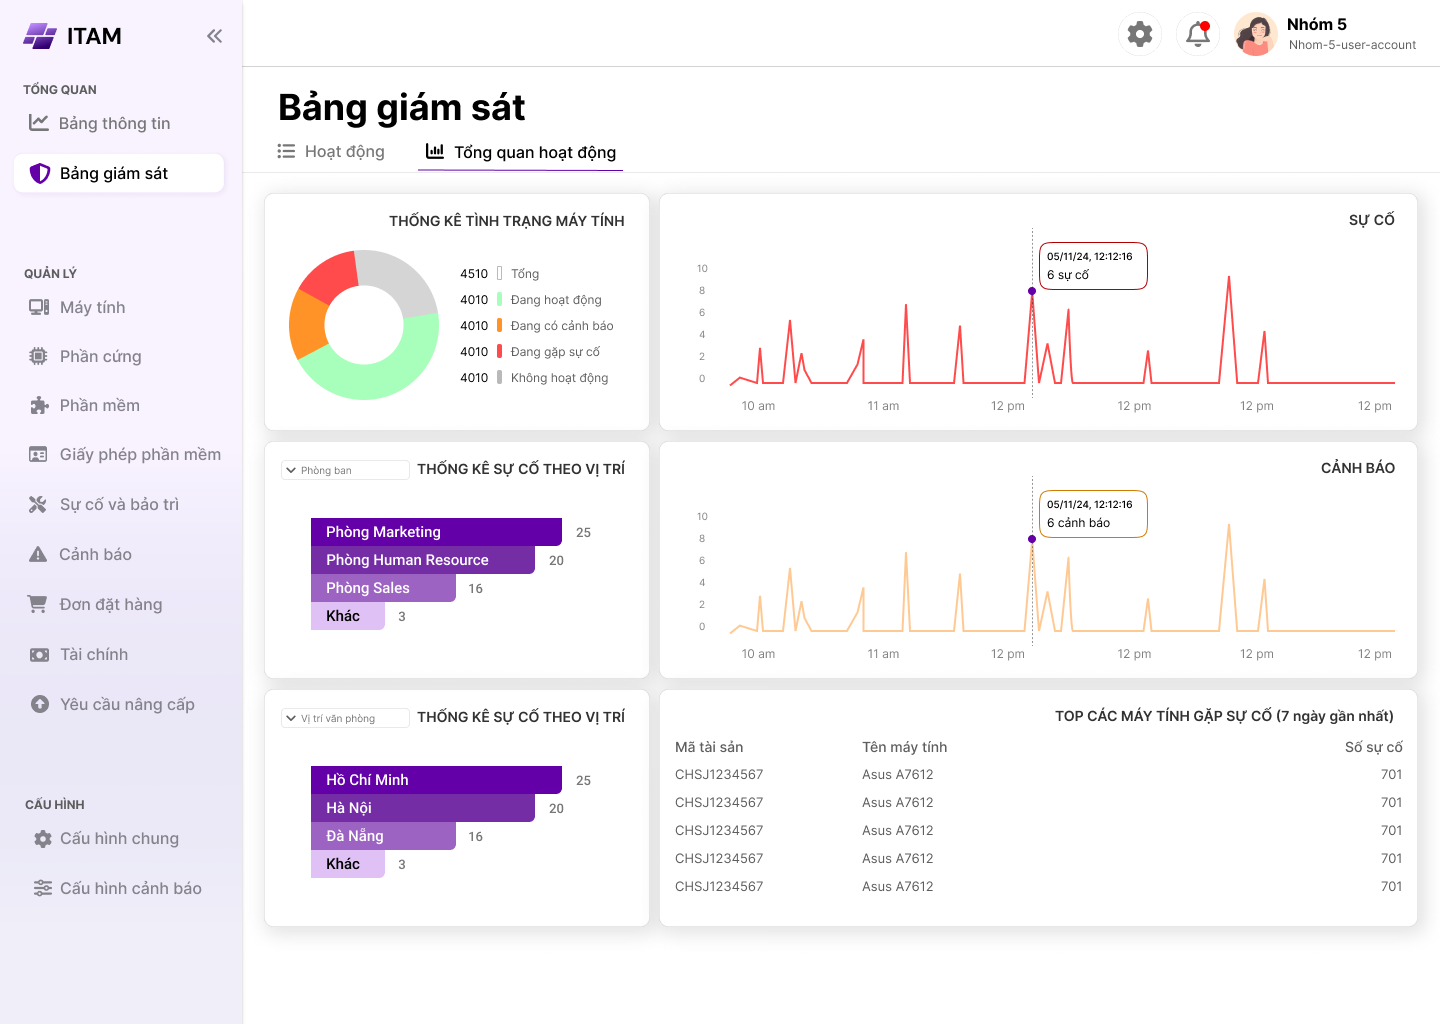
\includegraphics[width=14cm]{Images/C5/UI/Feature-Bảng giám sát 2.png}
%     \vspace{15pt}
%     \caption{Giao diện Bảng giám sát 3}
% \end{figure}

\item{Quản lý máy tính}\\
Quản lý máy tính cung cấp các tính năng cơ bản như xem danh sách máy tính, xem thông tin chi tiết máy tính, chỉnh sửa thông tin chi tiết máy tính, thêm máy tính, gửi yêu cầu nâng cấp, gửi yêu cầu bảo trì, và xem báo cáo tổng quan về máy tính trong hệ thống.\\
Thông tin chi tiết của máy tính gồm:
\begin{itemize}
    \item Thông tin chung như tên, số serial, loại máy tính, địa chỉ MAC,...
    \item Thông tin phần cứng của máy tính
    \item Thông tin phần mềm của máy tính
    \item Thông tin vòng đời của máy tính (Mua sắm, triển khai, sử dung, thanh lý)
    \item Hiệu suất sử dụng
\end{itemize}
% \begin{figure}[H]
%     \centering
%     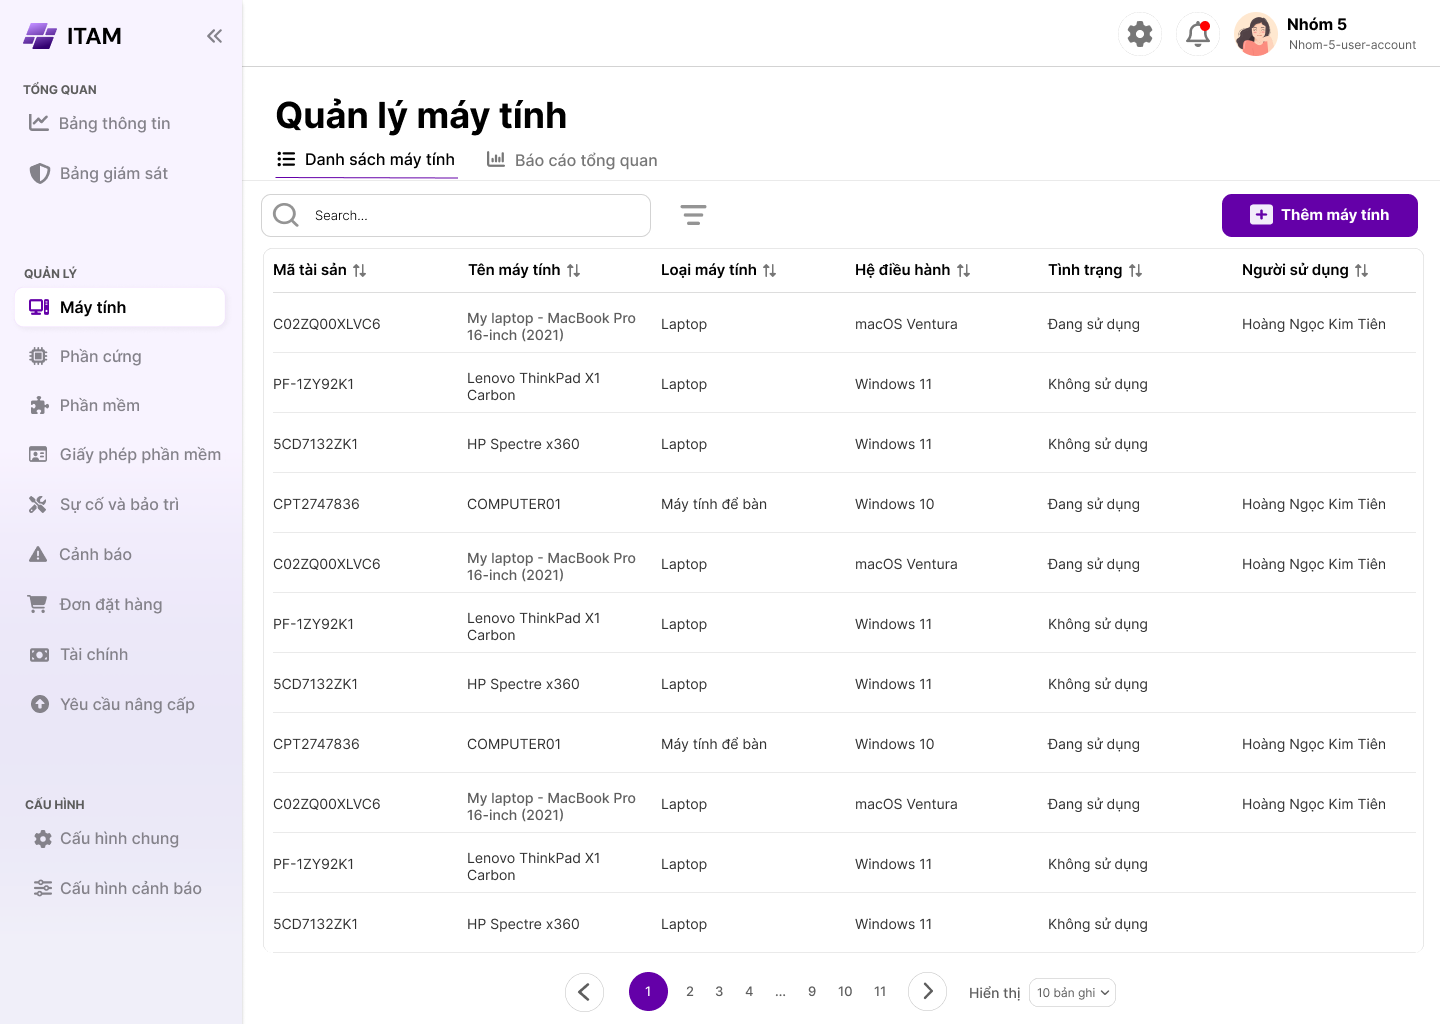
\includegraphics[width=14cm]{Images/C5/UI/Feature-Giám sát tài sản-Máy tính 1.1.png}
%     \vspace{15pt}
%     \caption{Giao diện Quản lý máy tính 1}
% \end{figure}
% \begin{figure}[H]
%     \centering
%     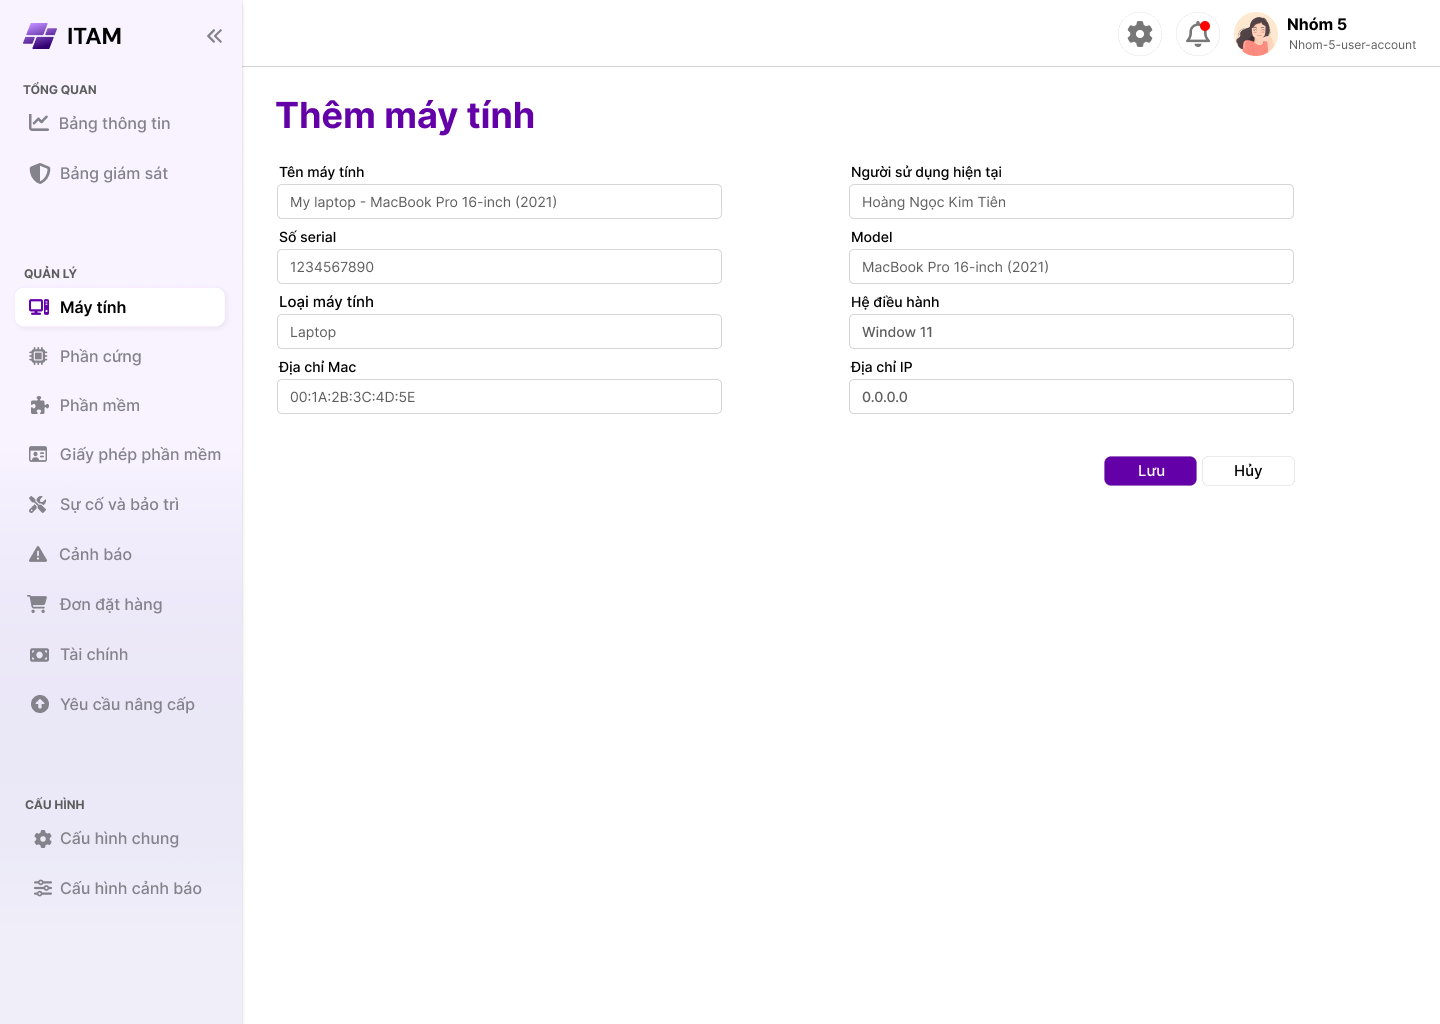
\includegraphics[width=14cm]{Images/C5/UI/Feature-Giám sát tài sản-Máy tính 1.2.png}
%     \vspace{15pt}
%     \caption{Giao diện Quản lý máy tính 2}
% \end{figure}
\begin{figure}[H]
    \centering
    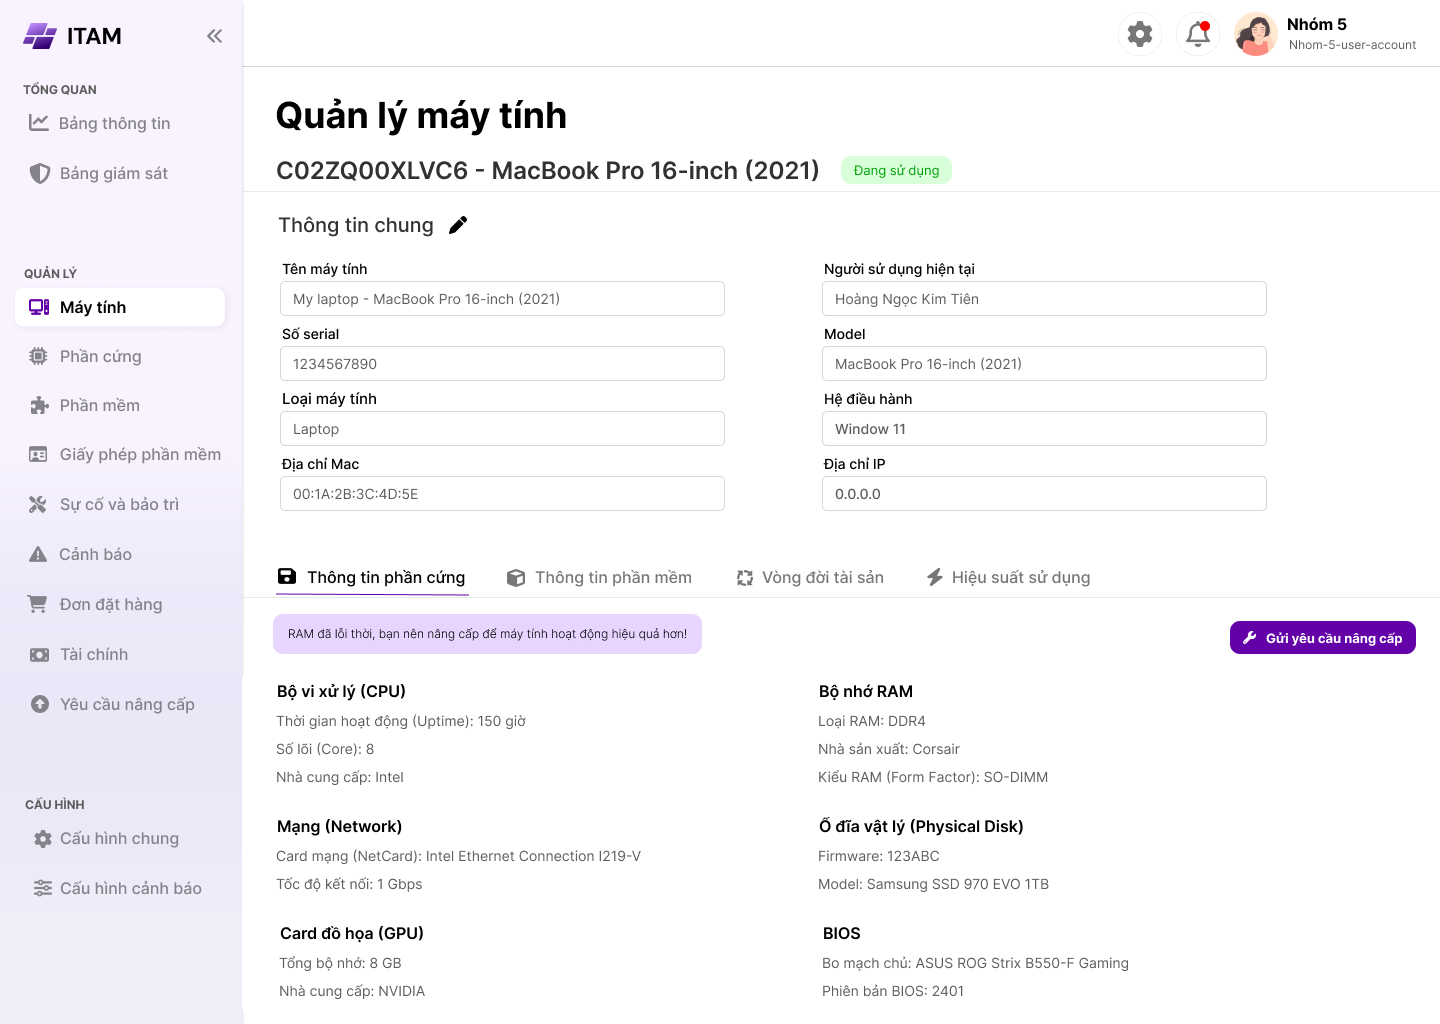
\includegraphics[width=14cm]{Images/C5/UI/Feature-Giám sát tài sản-Máy tính 2.1.png}
    \vspace{15pt}
    \caption{Giao diện Quản lý máy tính 1}
\end{figure}
% \begin{figure}[H]
%     \centering
%     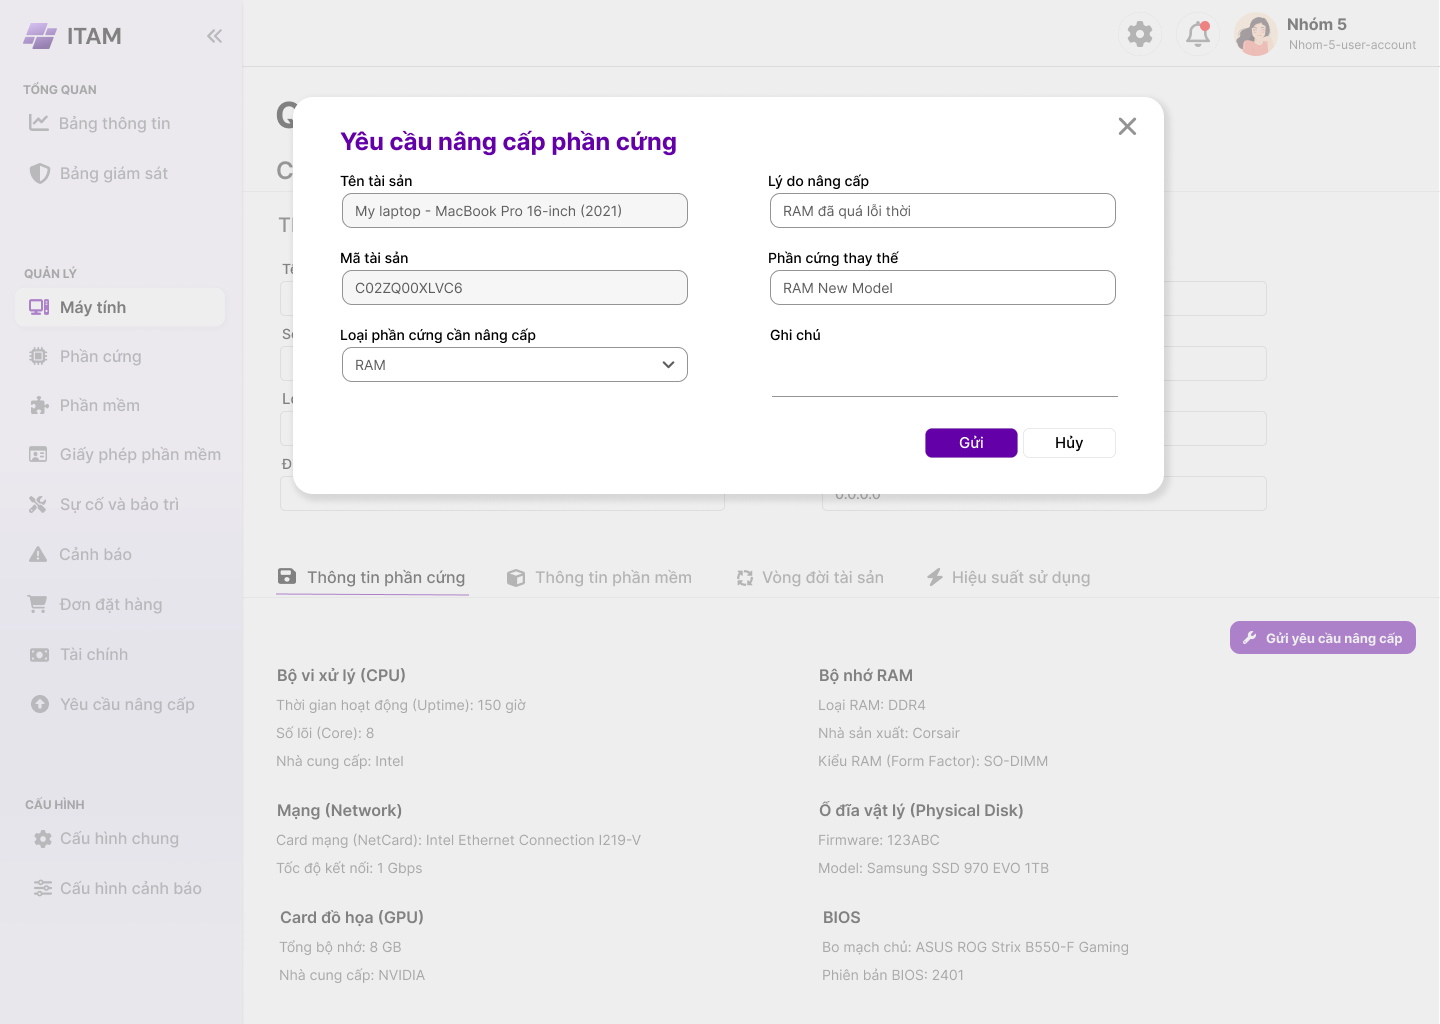
\includegraphics[width=14cm]{Images/C5/UI/Feature-Giám sát tài sản-Máy tính 2.2.png}
%     \vspace{15pt}
%     \caption{Giao diện Quản lý máy tính 4}
% \end{figure}
% \begin{figure}[H]
%     \centering
%     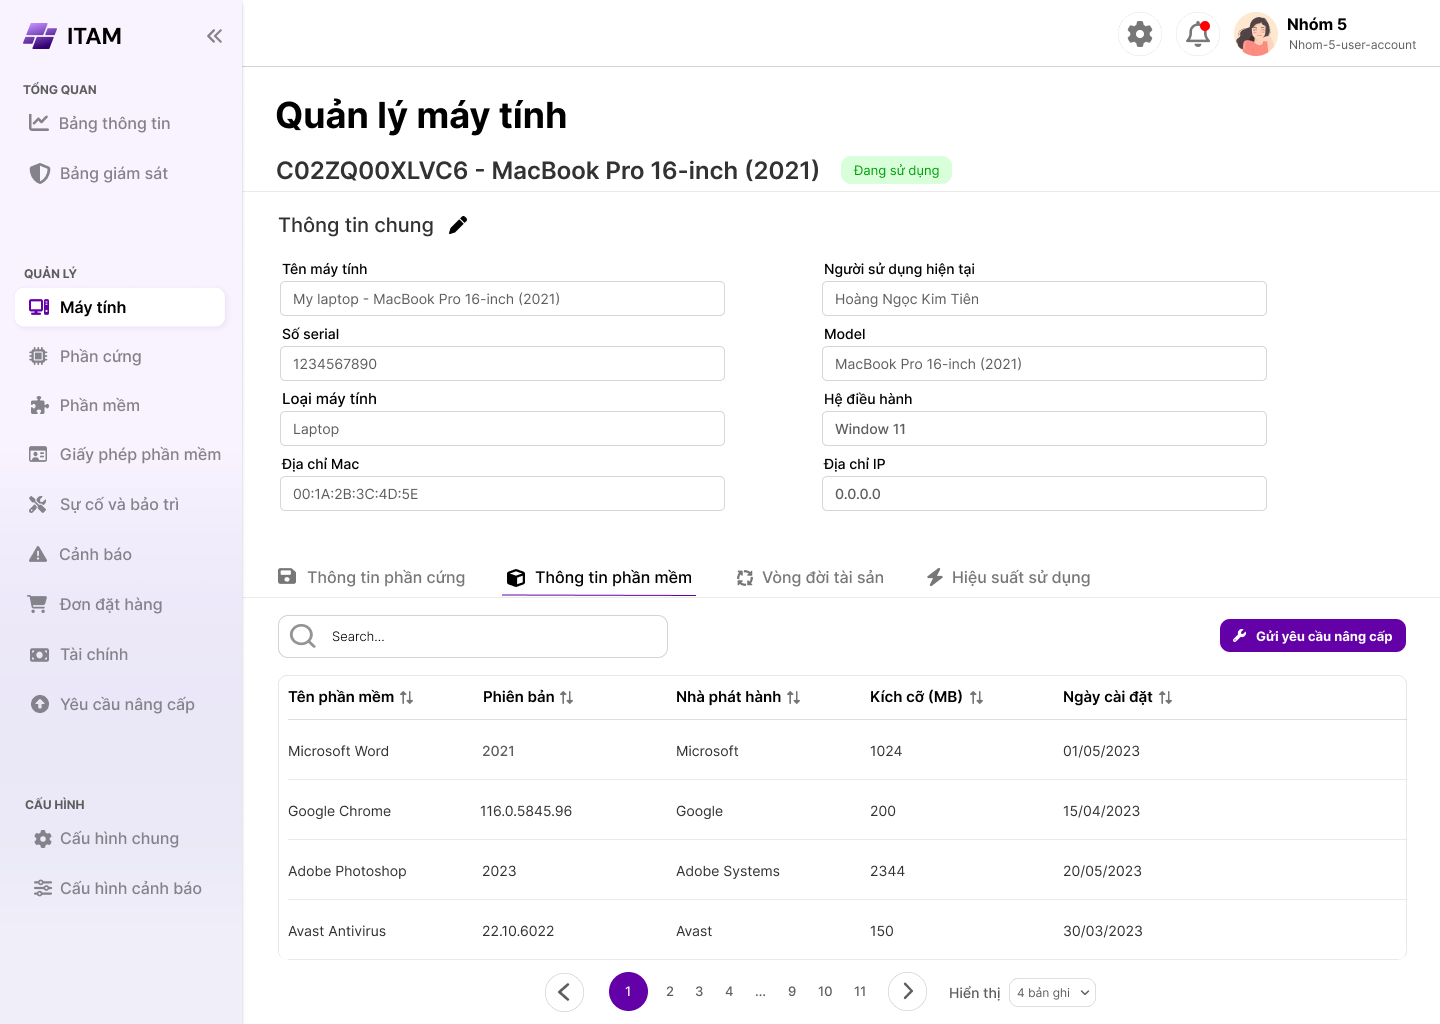
\includegraphics[width=14cm]{Images/C5/UI/Feature-Giám sát tài sản-Máy tính 3.1.png}
%     \vspace{15pt}
%     \caption{Giao diện Quản lý máy tính 5}
% \end{figure}
% \begin{figure}[H]
%     \centering
%     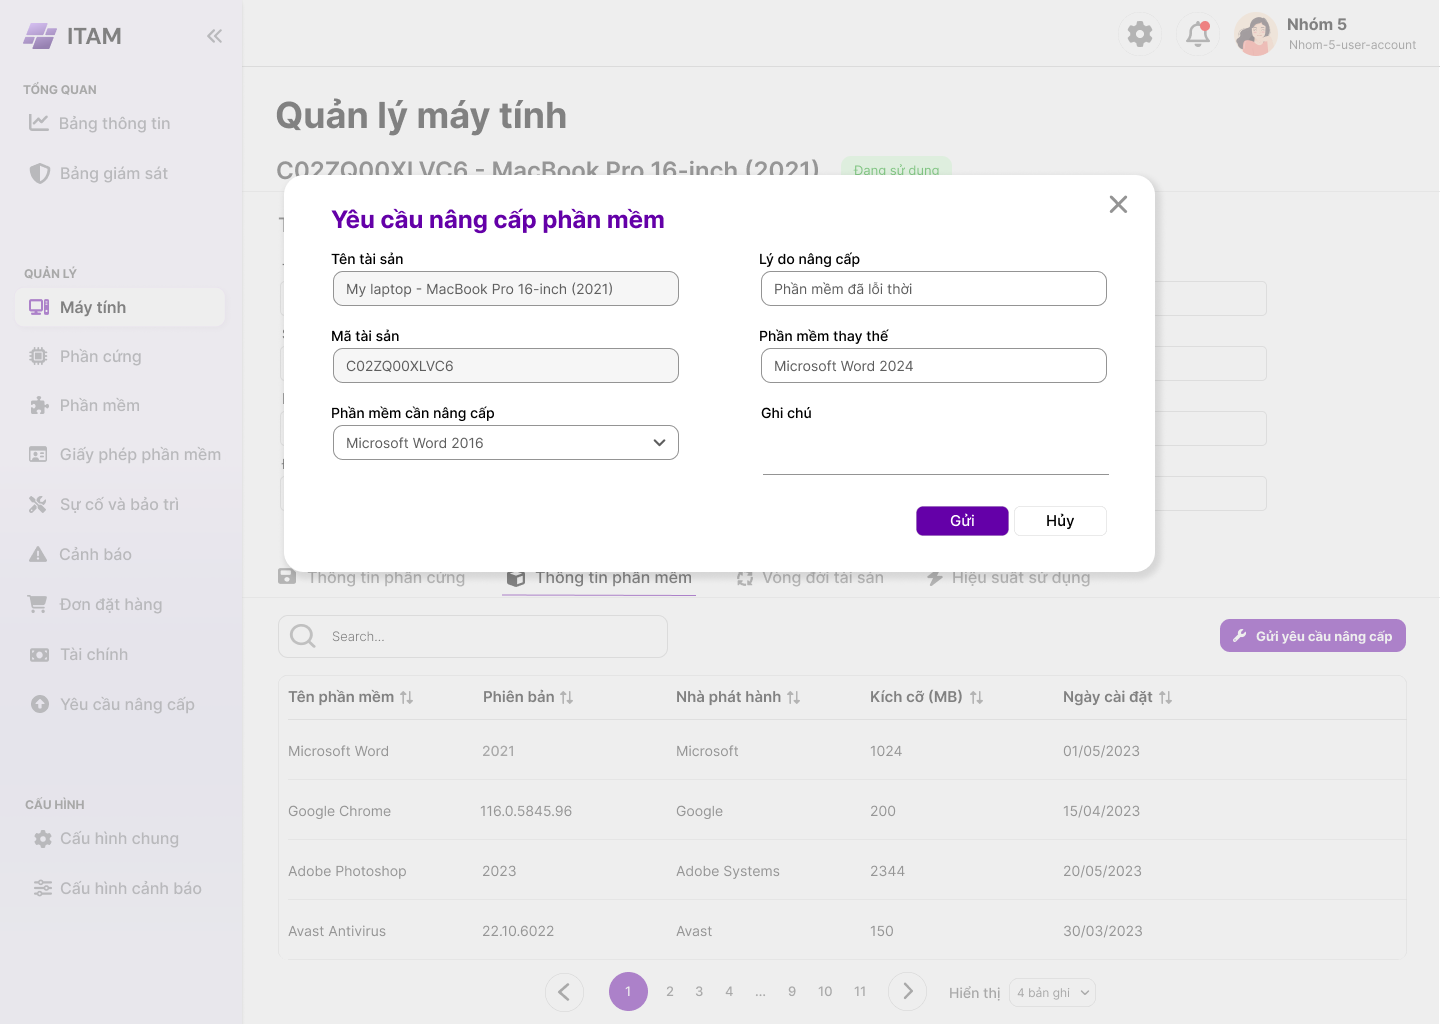
\includegraphics[width=14cm]{Images/C5/UI/Feature-Giám sát tài sản-Máy tính 3.2.png}
%     \vspace{15pt}
%     \caption{Giao diện Quản lý máy tính 6}
% \end{figure}
% \begin{figure}[H]
%     \centering
%     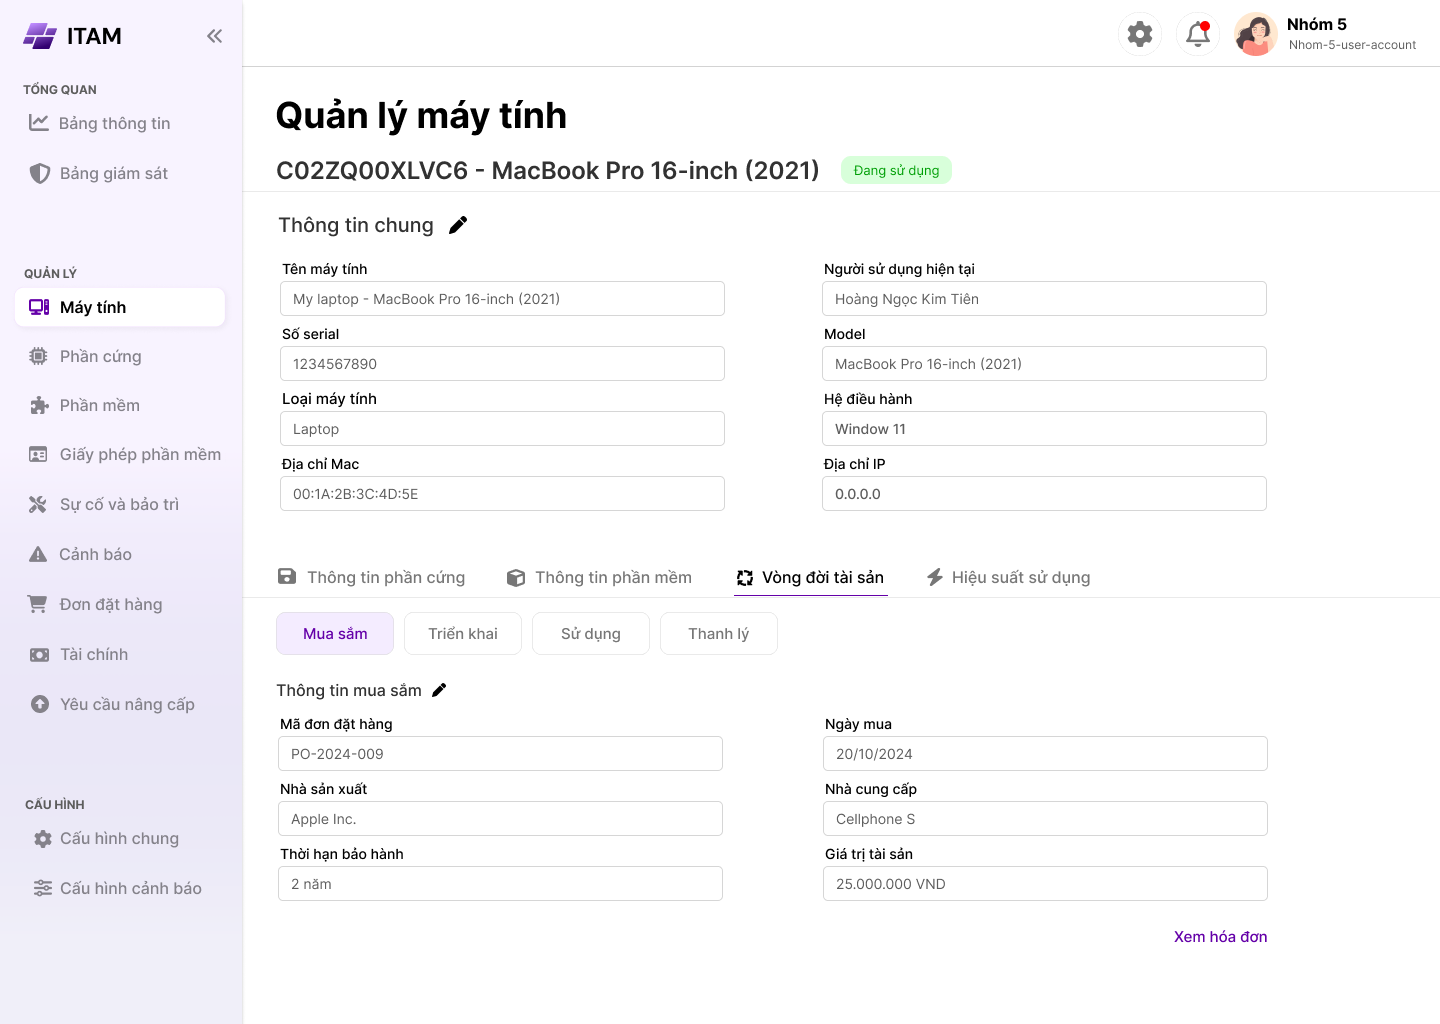
\includegraphics[width=14cm]{Images/C5/UI/Feature-Giám sát tài sản-Máy tính 4.1.png}
%     \vspace{15pt}
%     \caption{Giao diện Quản lý máy tính 7}
% \end{figure}
% \begin{figure}[H]
%     \centering
%     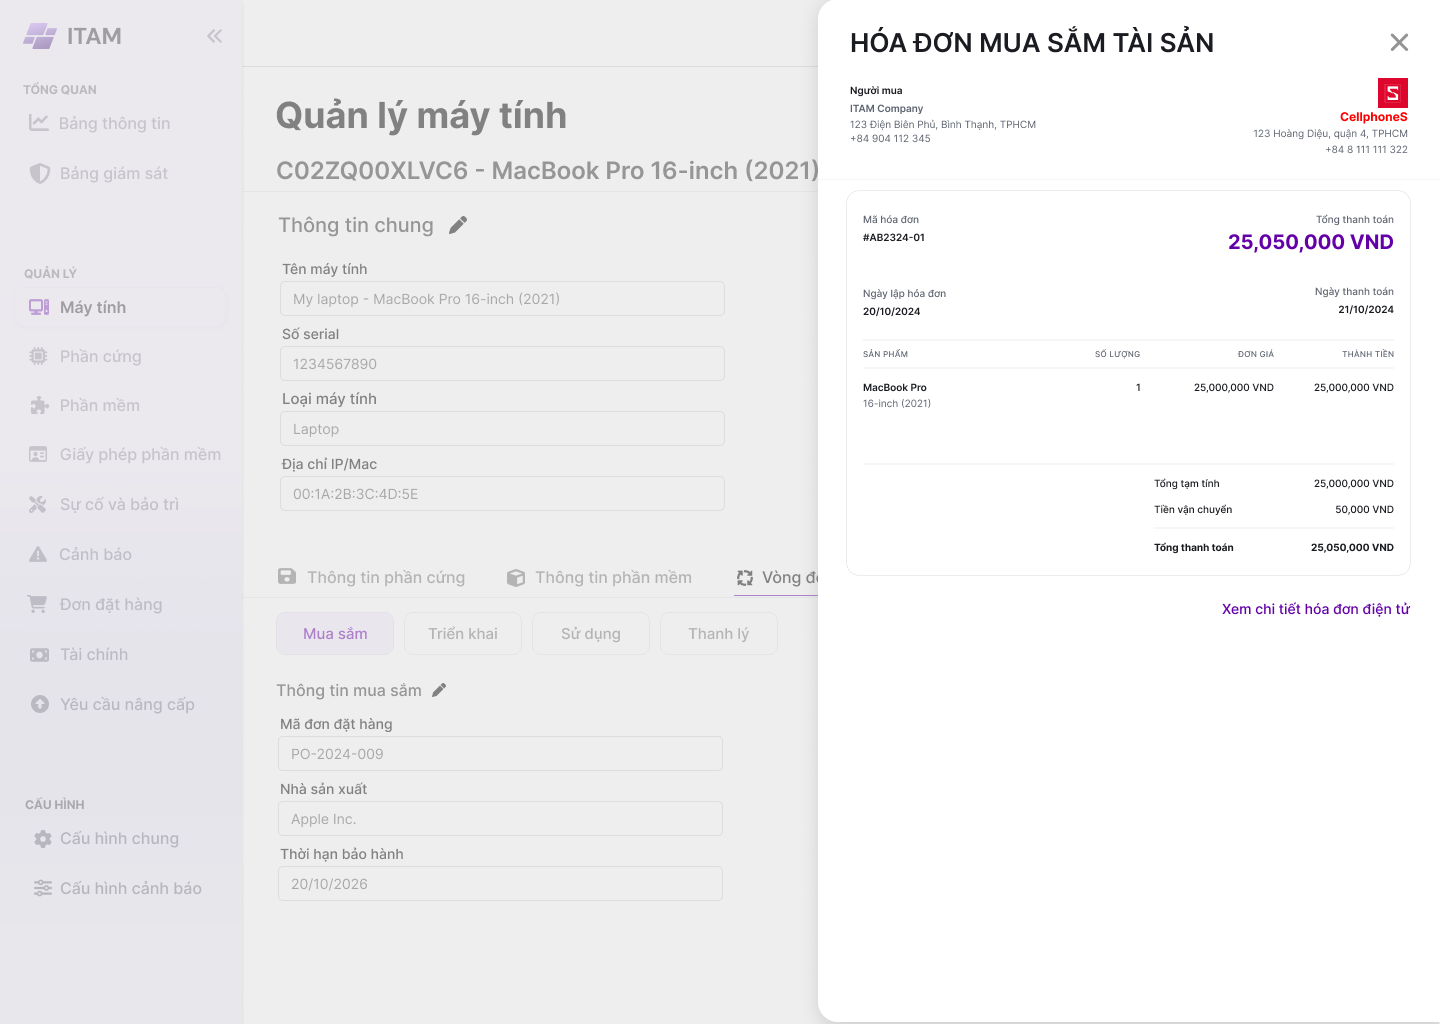
\includegraphics[width=14cm]{Images/C5/UI/Feature-Giám sát tài sản-Máy tính 4.2.png}
%     \vspace{15pt}
%     \caption{Giao diện Quản lý máy tính 8}
% \end{figure}
% \begin{figure}[H]
%     \centering
%     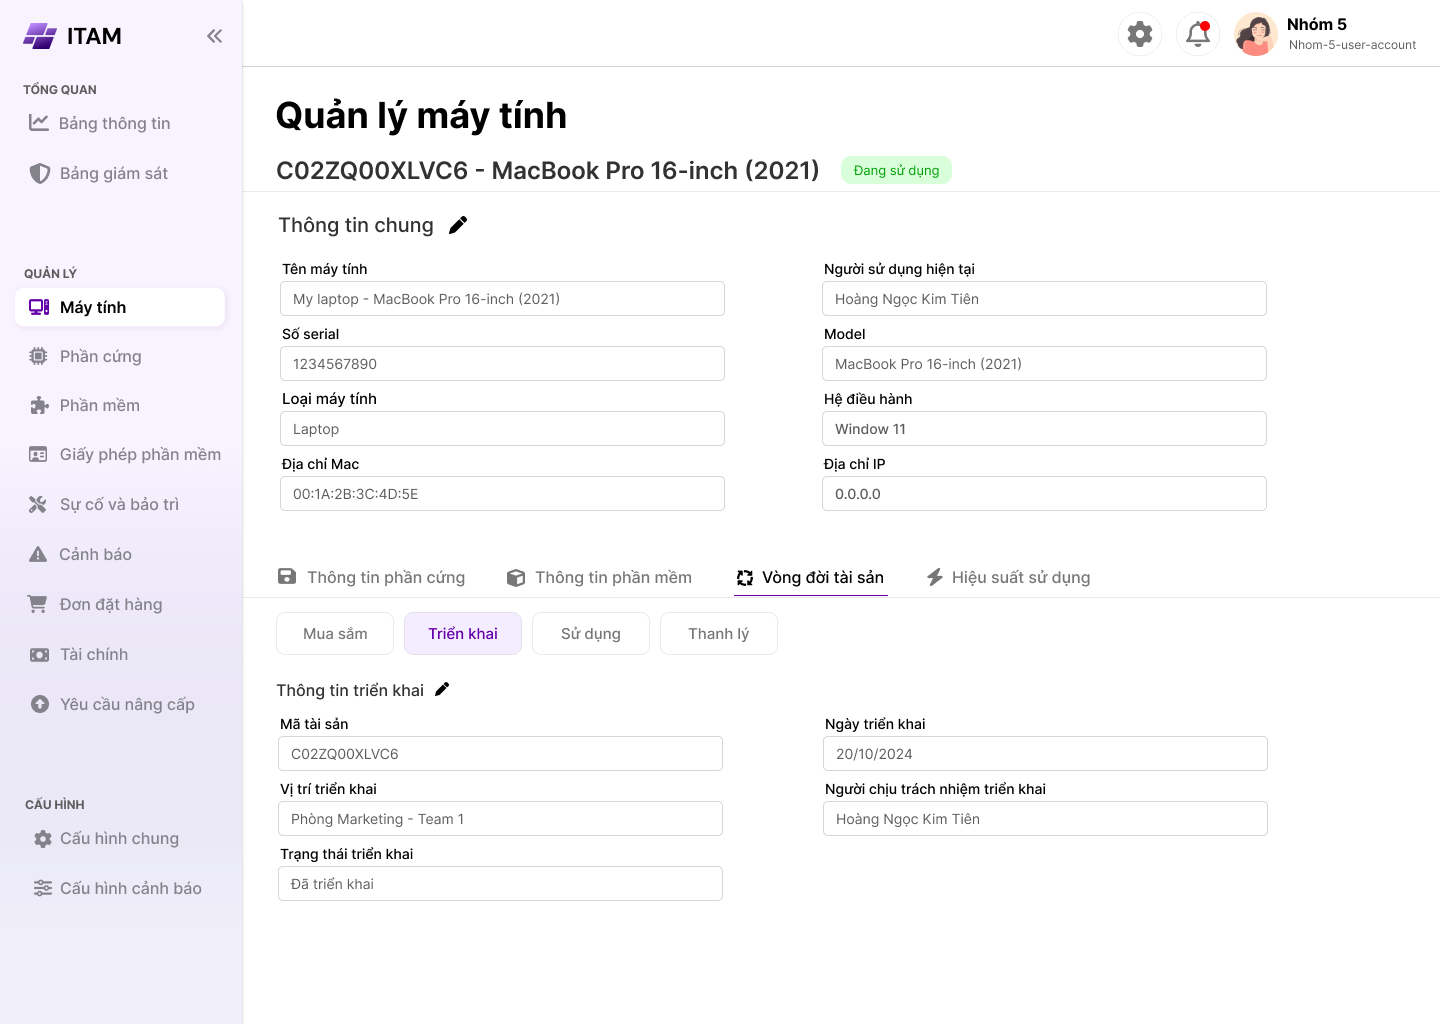
\includegraphics[width=14cm]{Images/C5/UI/Feature-Giám sát tài sản-Máy tính 5.png}
%     \vspace{15pt}
%     \caption{Giao diện Quản lý máy tính 8}
% \end{figure}
% \begin{figure}[H]
%     \centering
%     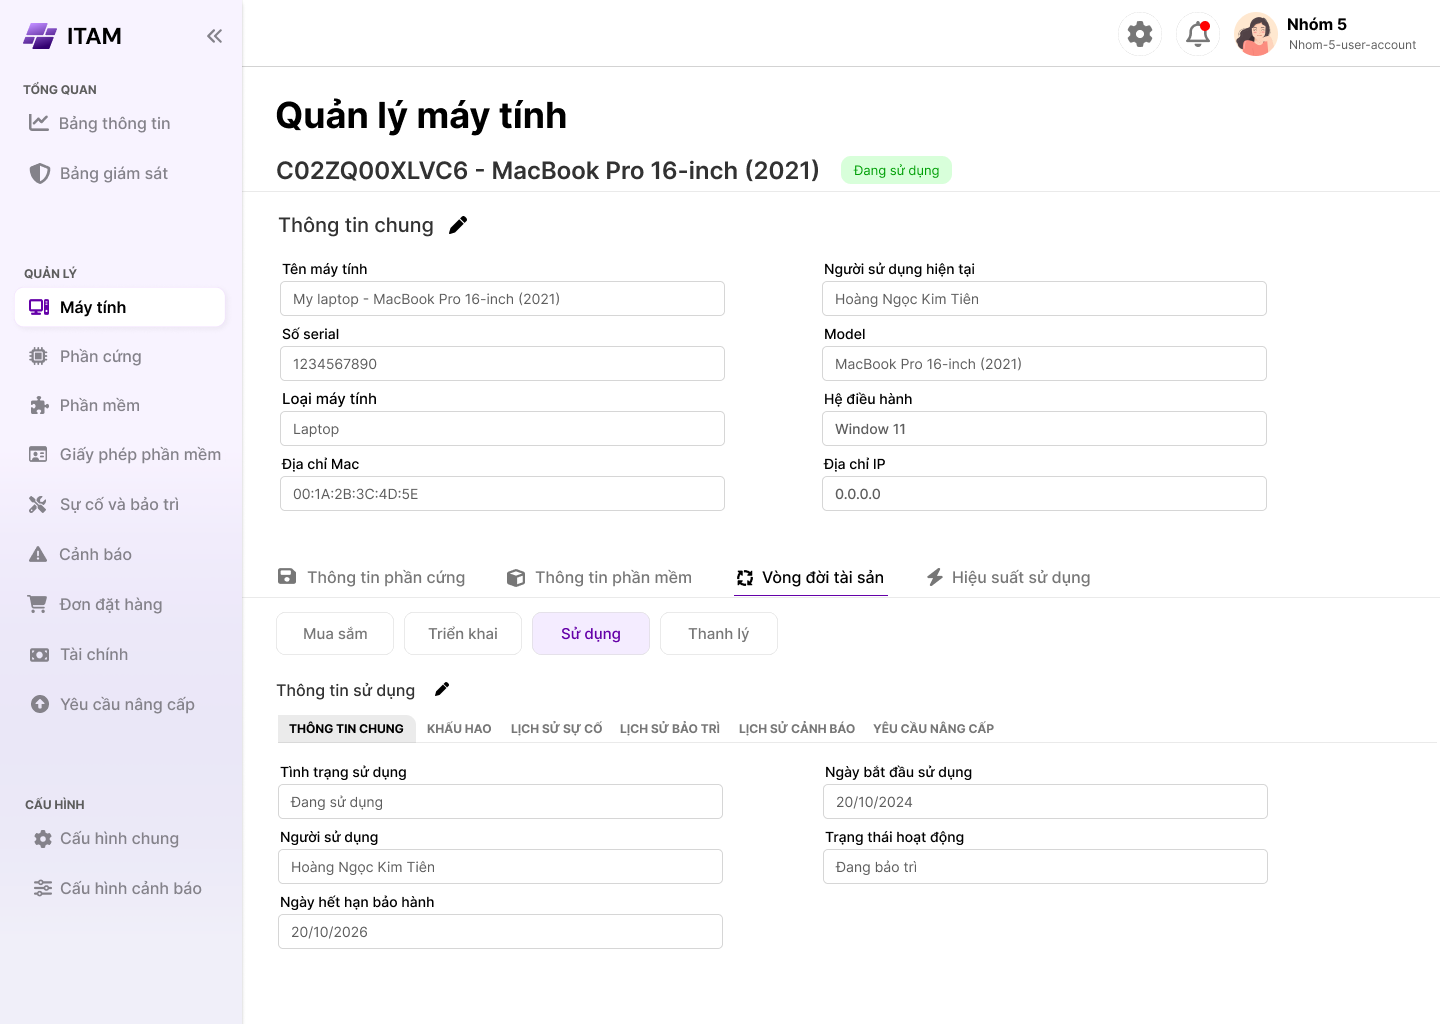
\includegraphics[width=14cm]{Images/C5/UI/Feature-Giám sát tài sản-Máy tính 6.1.png}
%     \vspace{15pt}
%     \caption{Giao diện Quản lý máy tính 9}
% \end{figure}
% \begin{figure}[H]
%     \centering
%     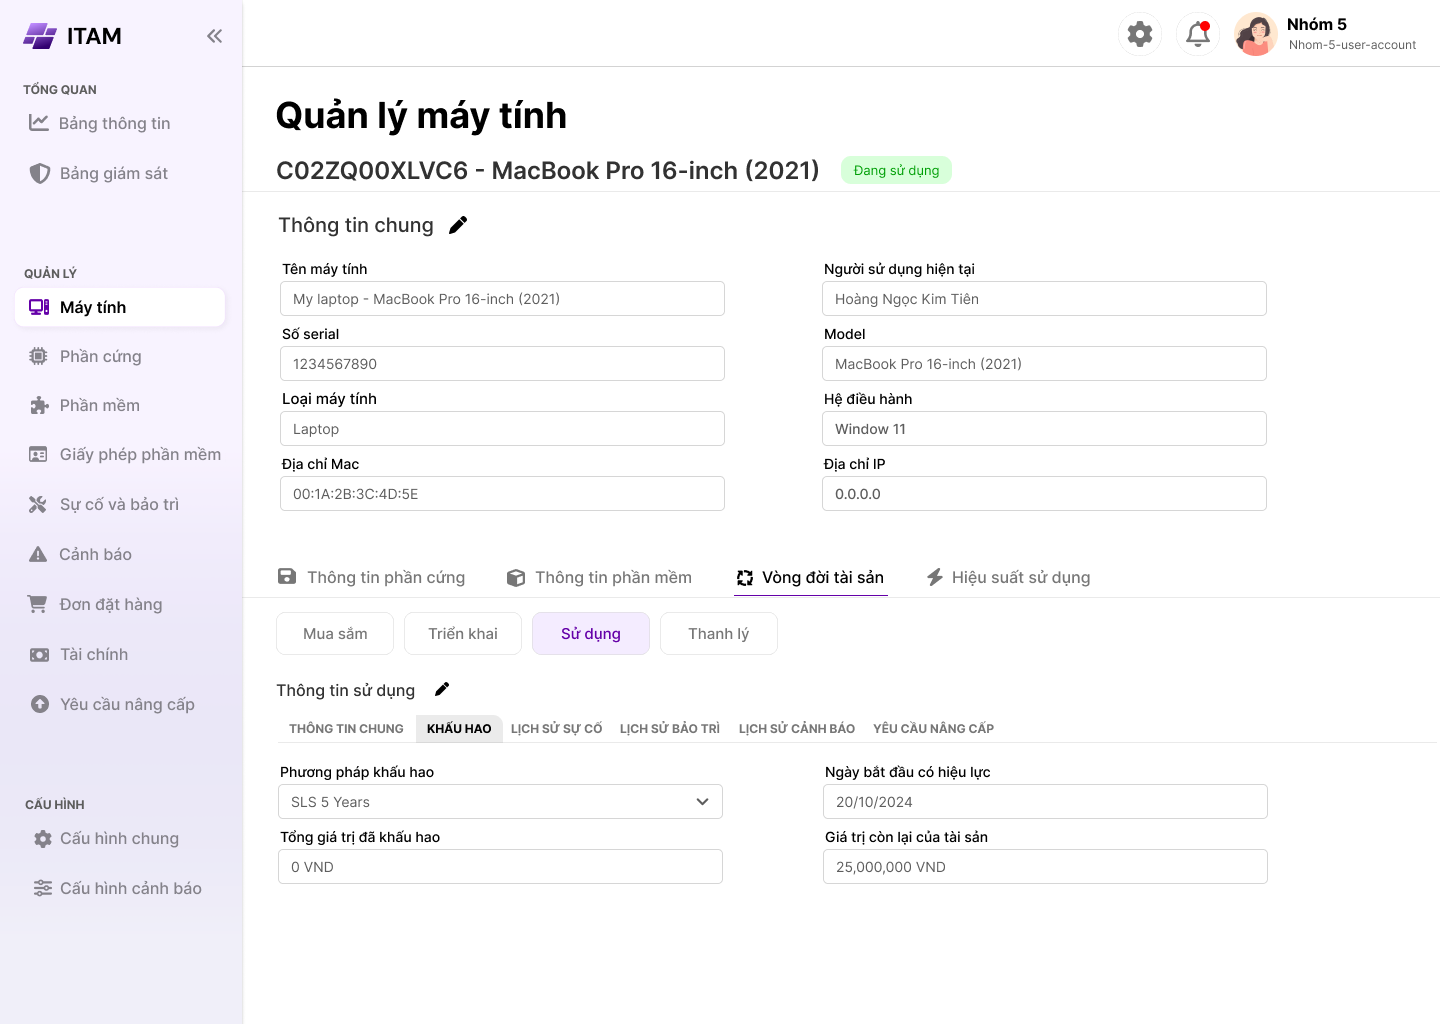
\includegraphics[width=14cm]{Images/C5/UI/Feature-Giám sát tài sản-Máy tính 6.2.png}
%     \vspace{15pt}
%     \caption{Giao diện Quản lý máy tính 11}
% \end{figure}
% \begin{figure}[H]
%     \centering
%     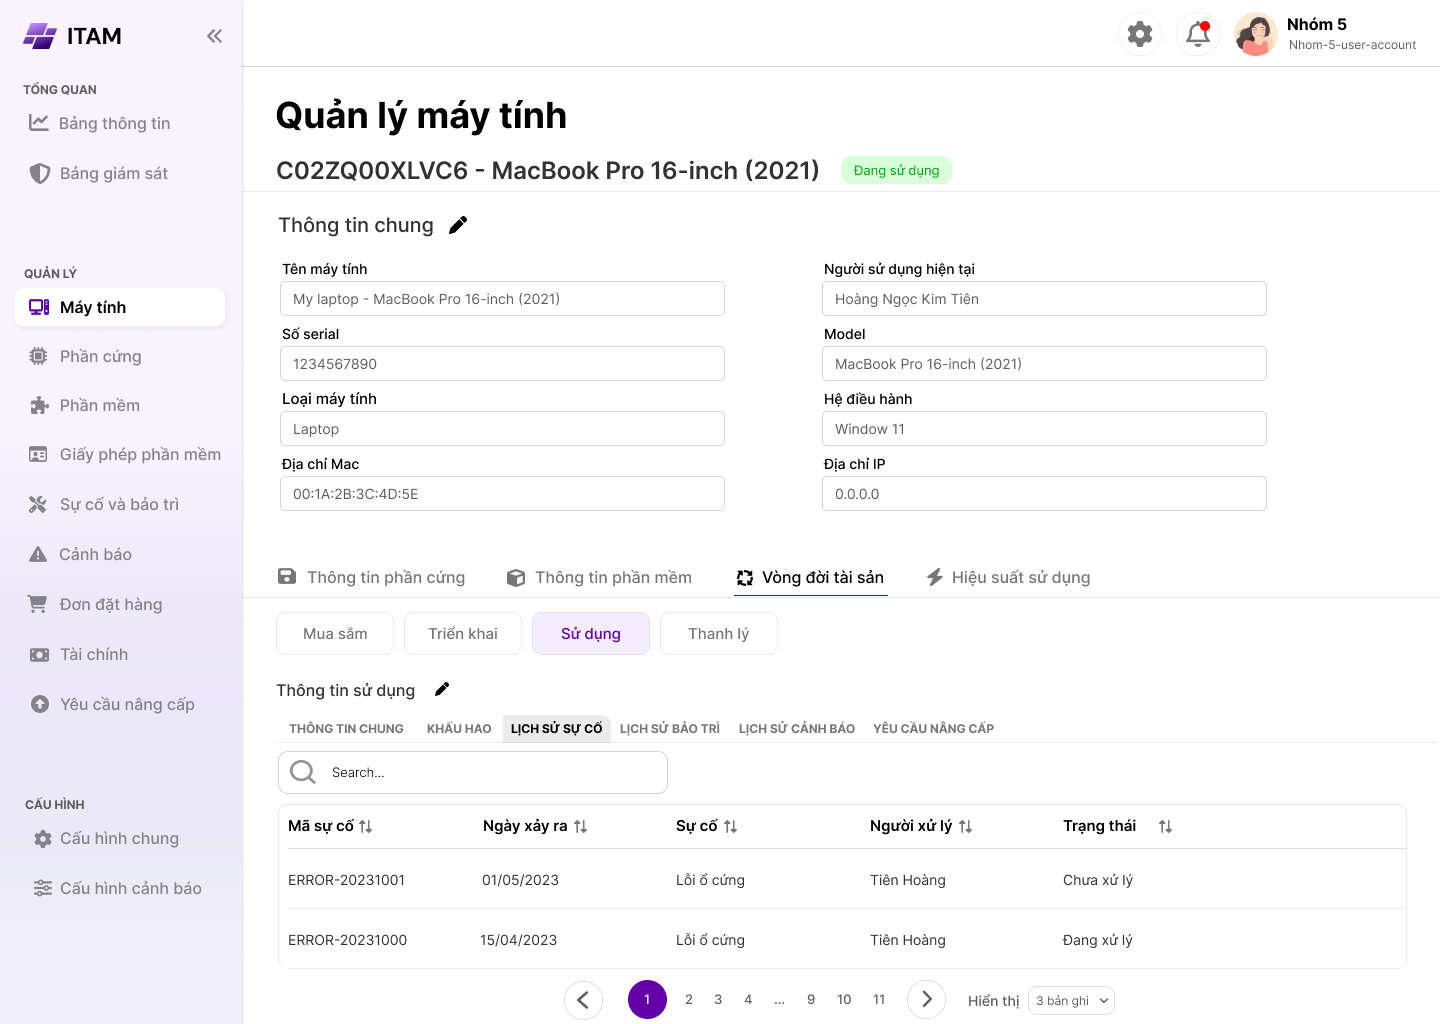
\includegraphics[width=14cm]{Images/C5/UI/Feature-Giám sát tài sản-Máy tính 6.3.png}
%     \vspace{15pt}
%     \caption{Giao diện Quản lý máy tính 12}
% \end{figure}
% \begin{figure}[H]
%     \centering
%     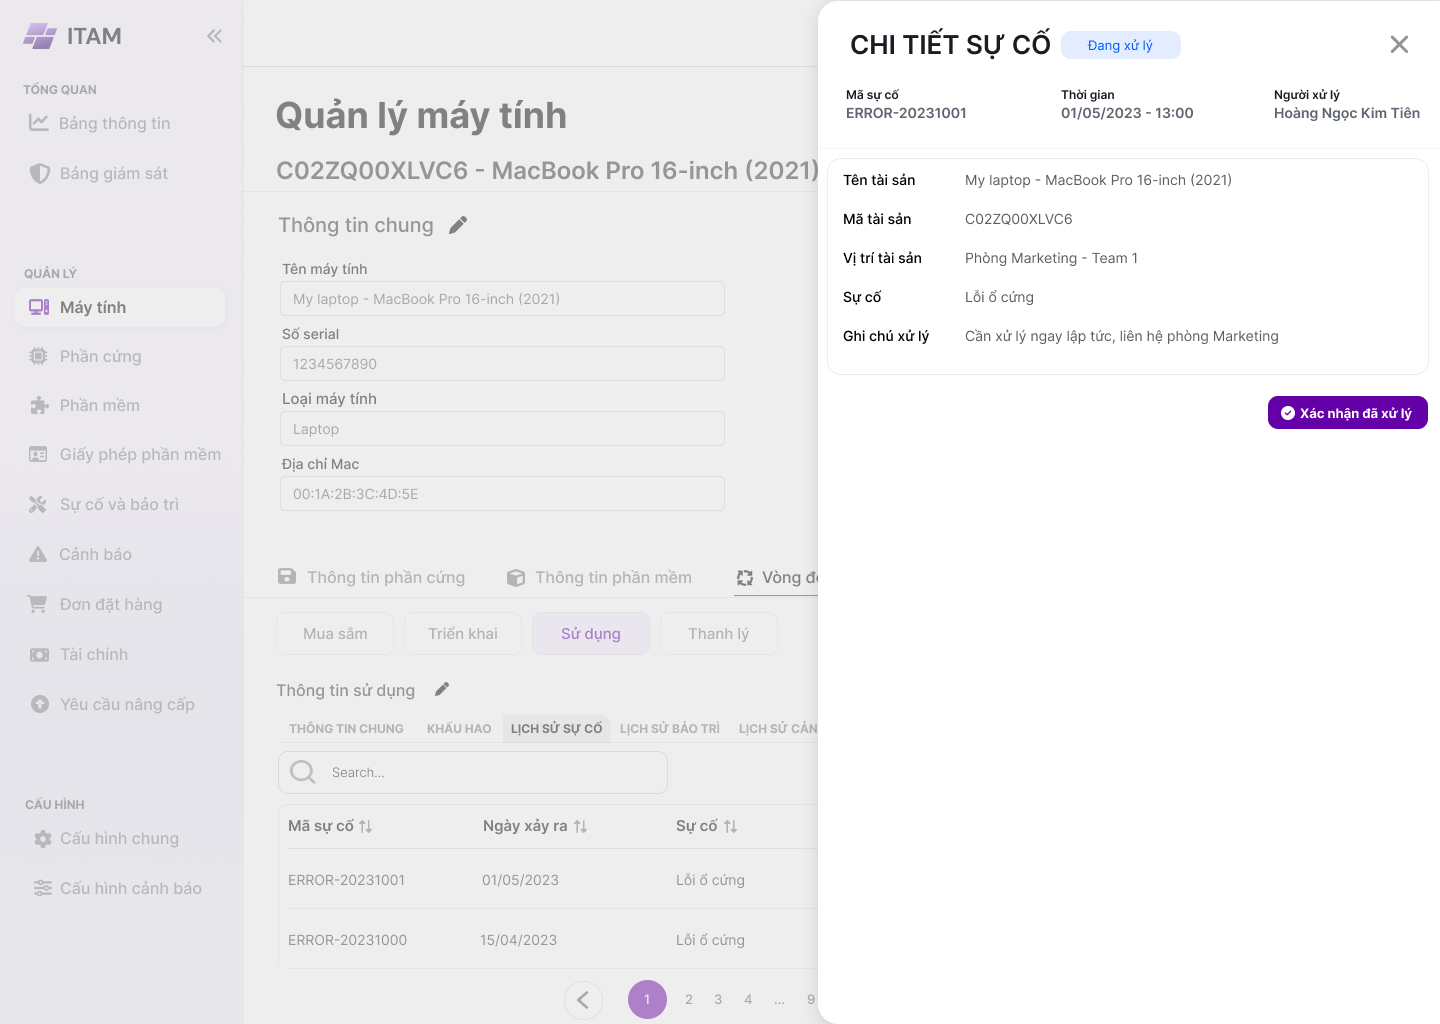
\includegraphics[width=14cm]{Images/C5/UI/Feature-Giám sát tài sản-Máy tính 6.4.png}
%     \vspace{15pt}
%     \caption{Giao diện Quản lý máy tính 13}
% \end{figure}
% \begin{figure}[H]
%     \centering
%     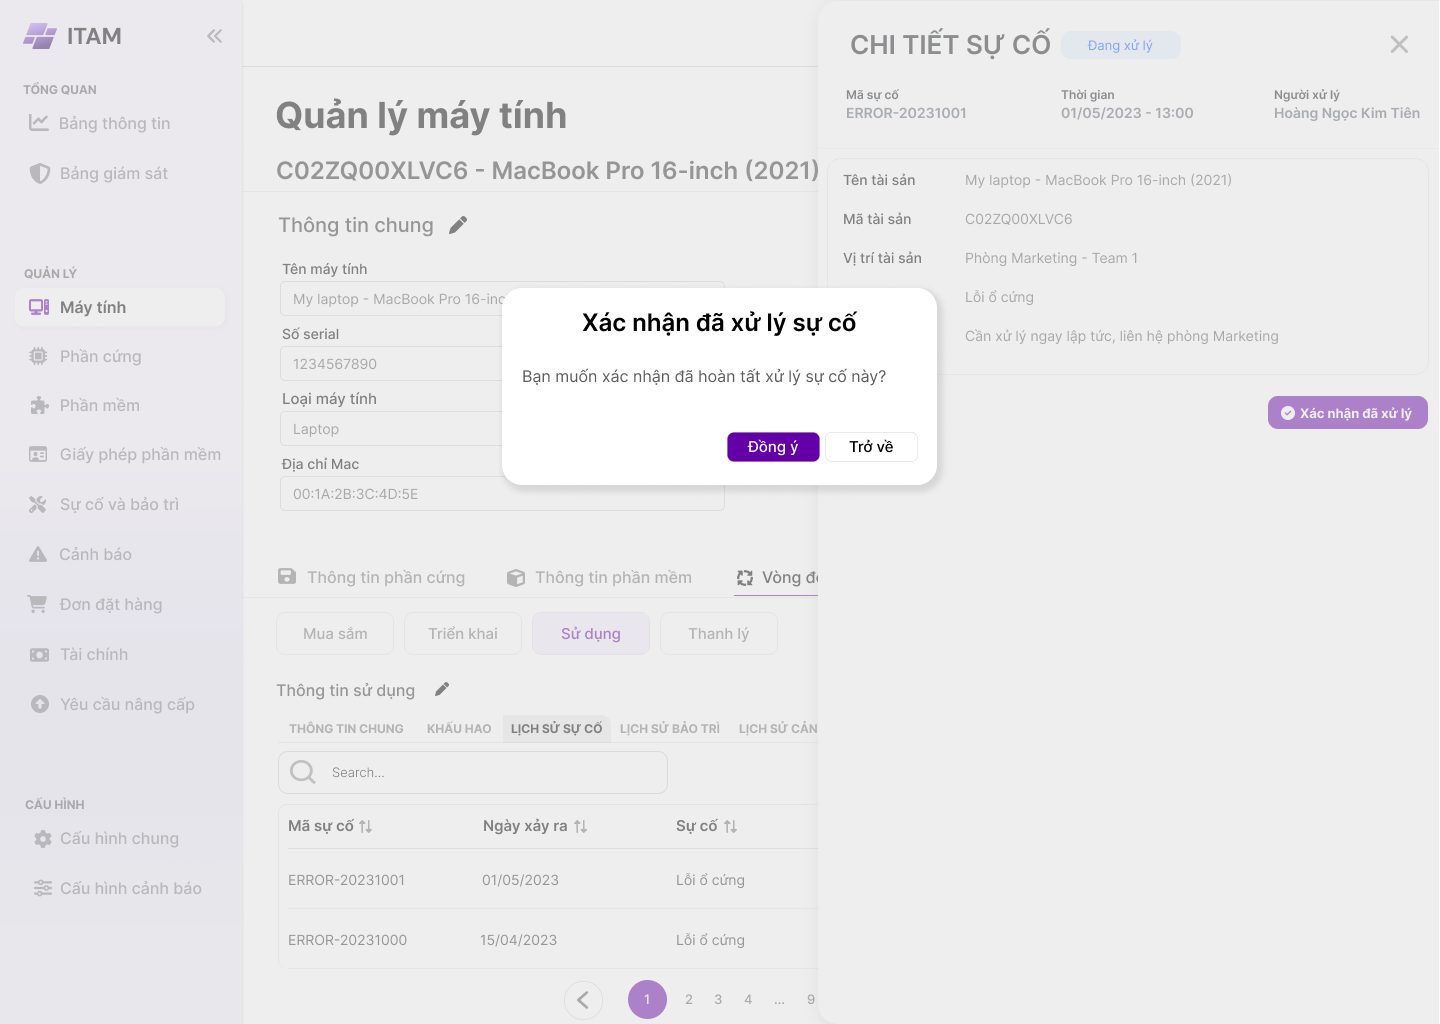
\includegraphics[width=14cm]{Images/C5/UI/Feature-Giám sát tài sản-Máy tính 6.5.png}
%     \vspace{15pt}
%     \caption{Giao diện Quản lý máy tính 14}
% \end{figure}
% \begin{figure}[H]
%     \centering
%     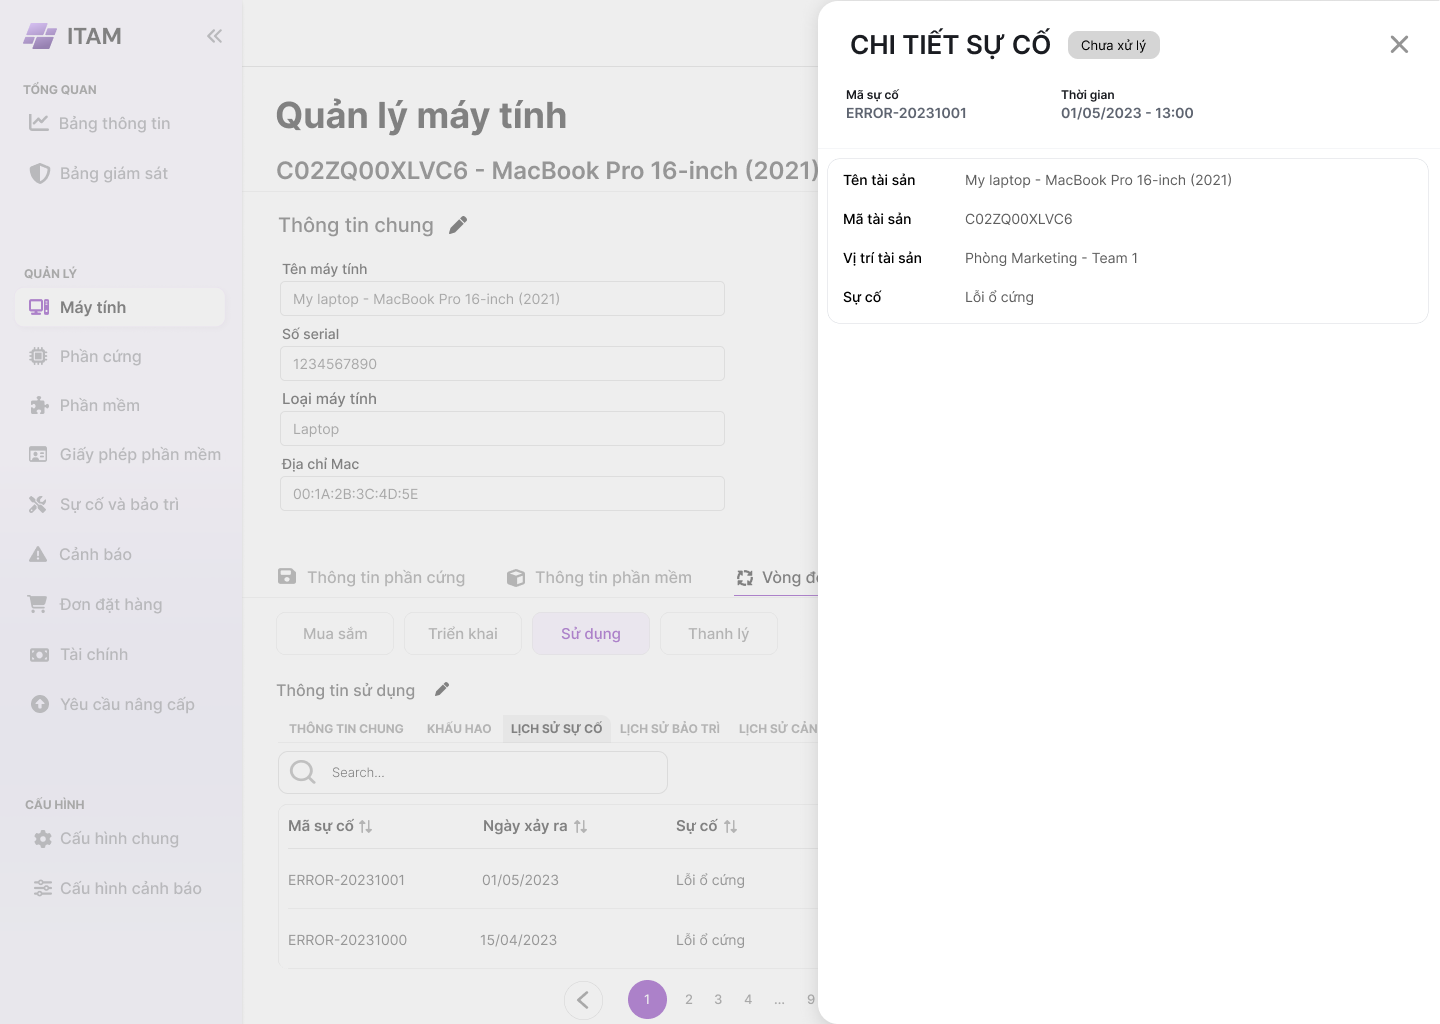
\includegraphics[width=14cm]{Images/C5/UI/Feature-Giám sát tài sản-Máy tính 6.6.png}
%     \vspace{15pt}
%     \caption{Giao diện Quản lý máy tính 15}
% \end{figure}
% \begin{figure}[H]
%     \centering
%     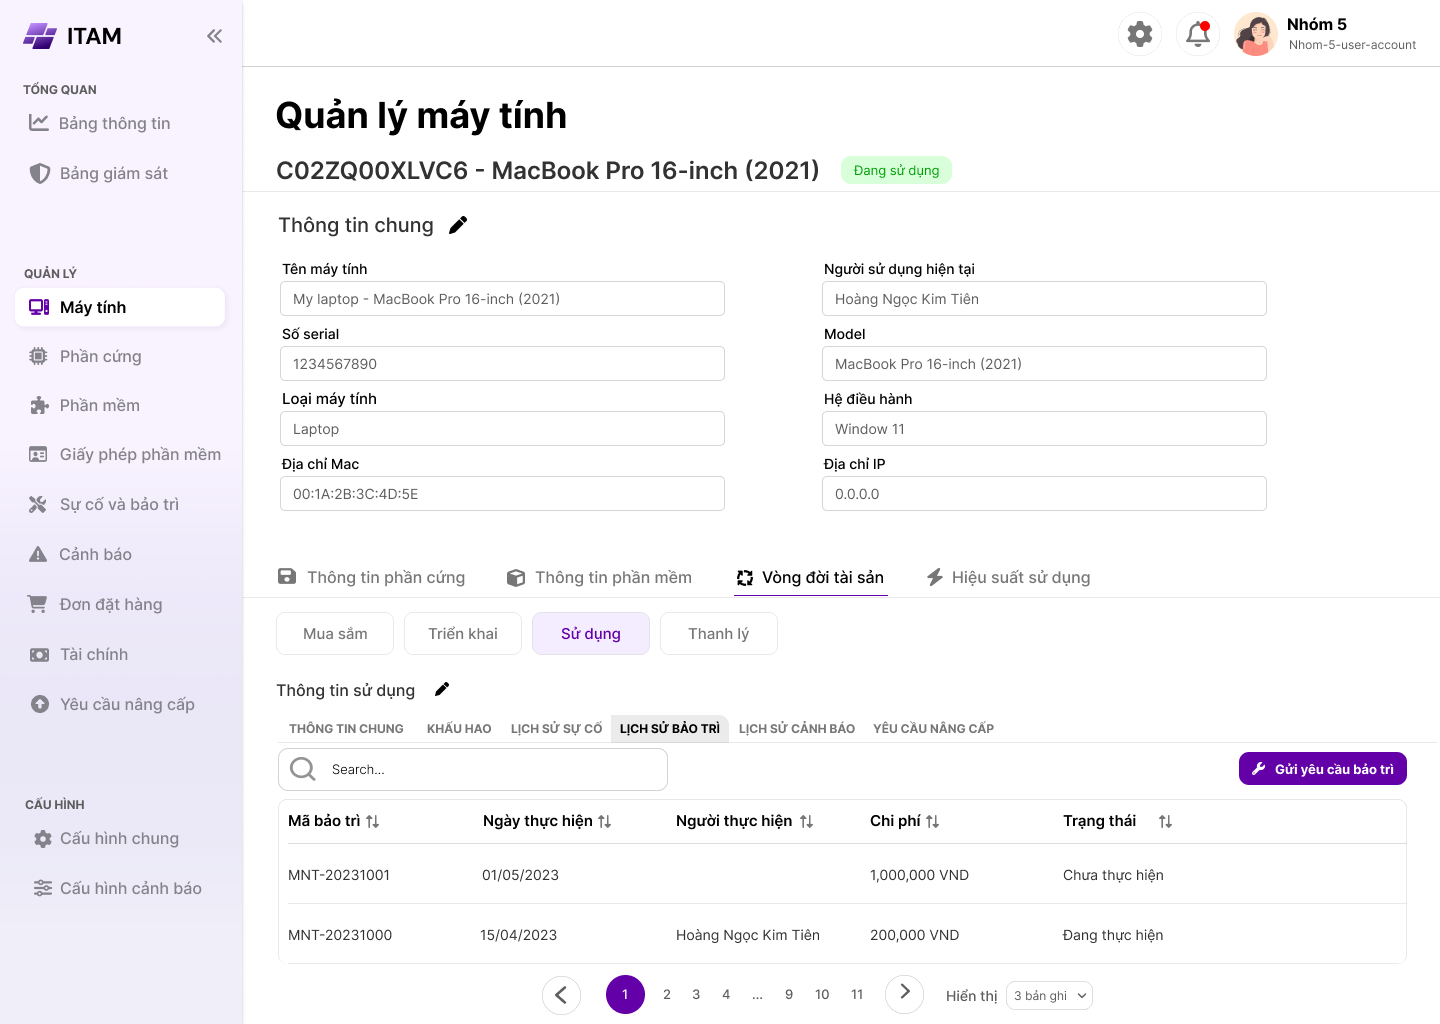
\includegraphics[width=14cm]{Images/C5/UI/Feature-Giám sát tài sản-Máy tính 6.8.png}
%     \vspace{15pt}
%     \caption{Giao diện Quản lý máy tính 10}
% \end{figure}
% \begin{figure}[H]
%     \centering
%     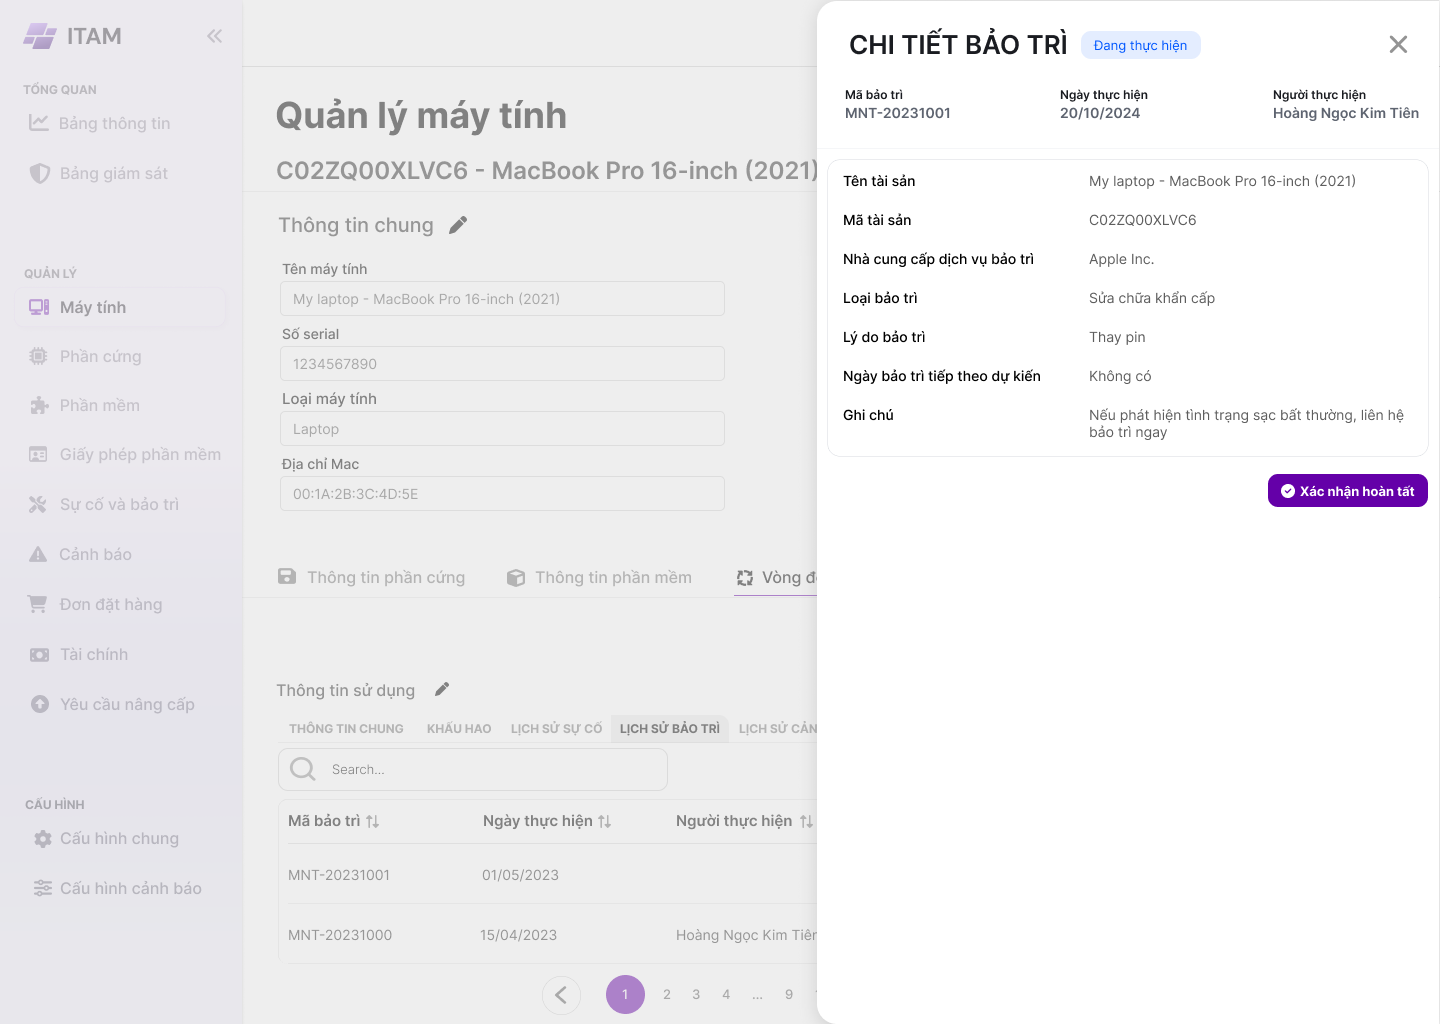
\includegraphics[width=14cm]{Images/C5/UI/Feature-Giám sát tài sản-Máy tính 6.9.png}
%     \vspace{15pt}
%     \caption{Giao diện Quản lý máy tính 17}
% \end{figure}
% \begin{figure}[H]
%     \centering
%     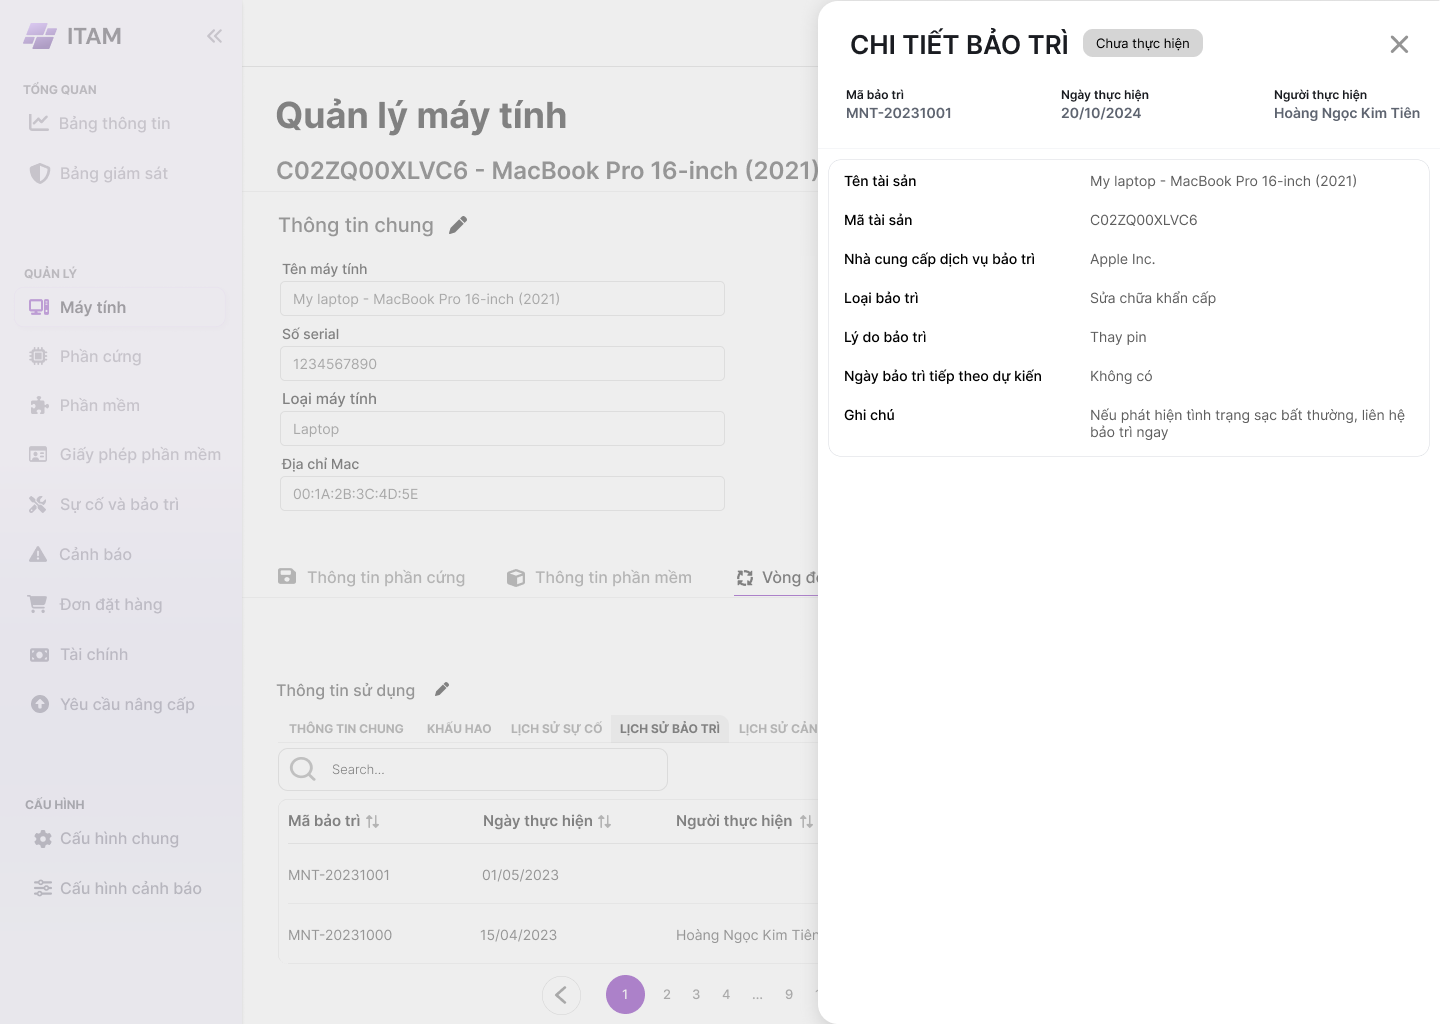
\includegraphics[width=14cm]{Images/C5/UI/Feature-Giám sát tài sản-Máy tính 6.10.png}
%     \vspace{15pt}
%     \caption{Giao diện Quản lý máy tính 18}
% \end{figure}
% \begin{figure}[H]
%     \centering
%     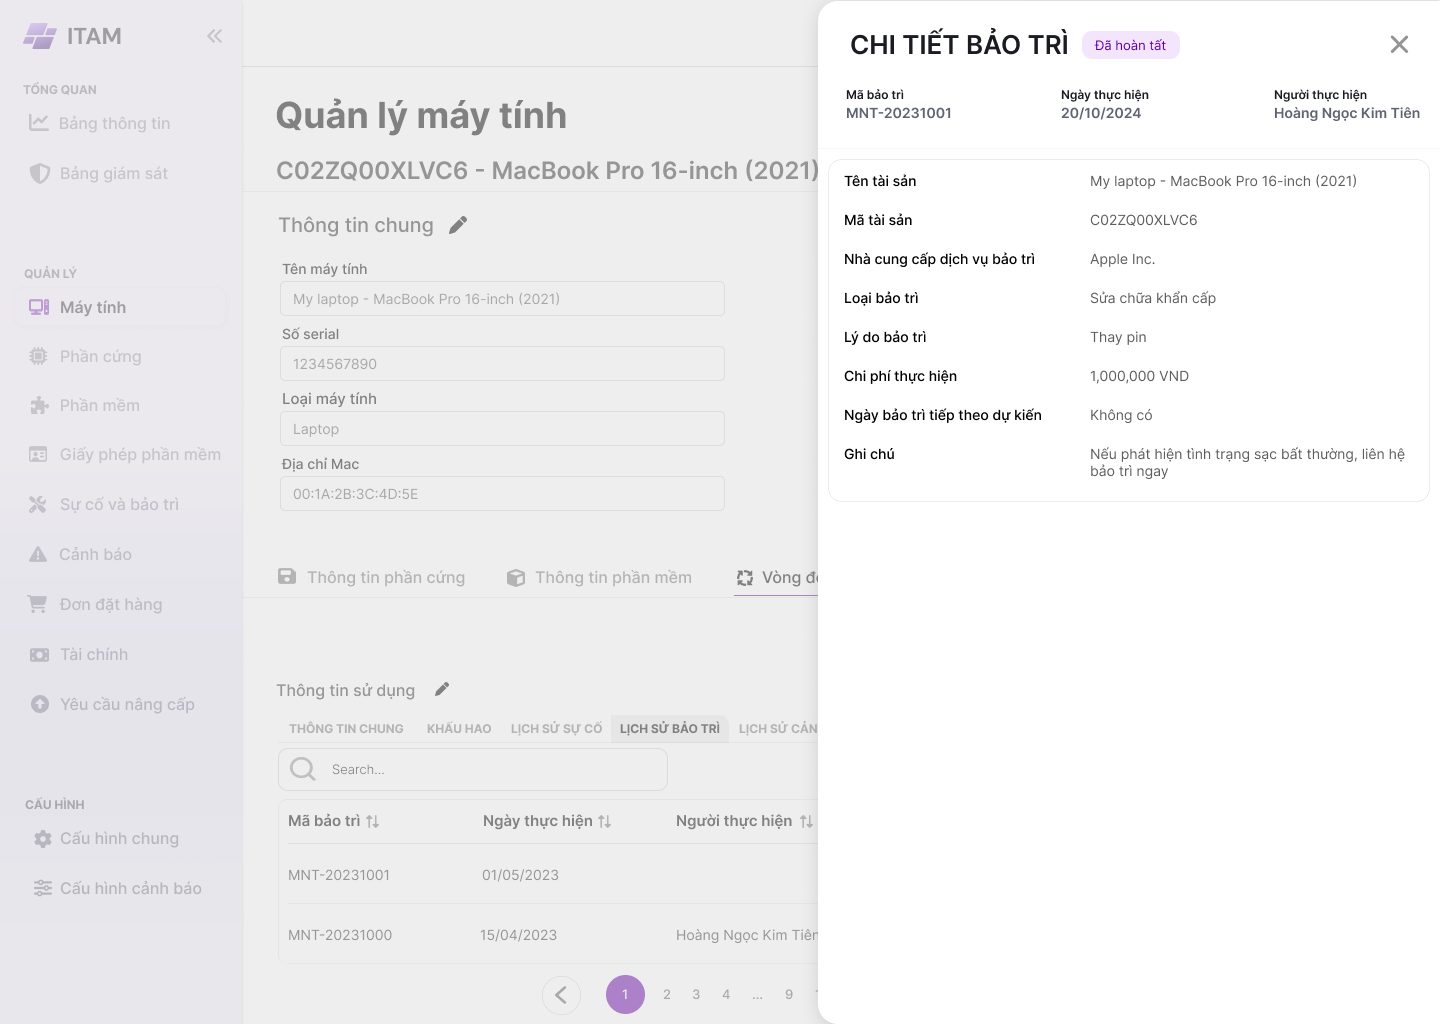
\includegraphics[width=14cm]{Images/C5/UI/Feature-Giám sát tài sản-Máy tính 6.11.png}
%     \vspace{15pt}
%     \caption{Giao diện Quản lý máy tính 19} 
% \end{figure}
% \begin{figure}[H]
%     \centering
%     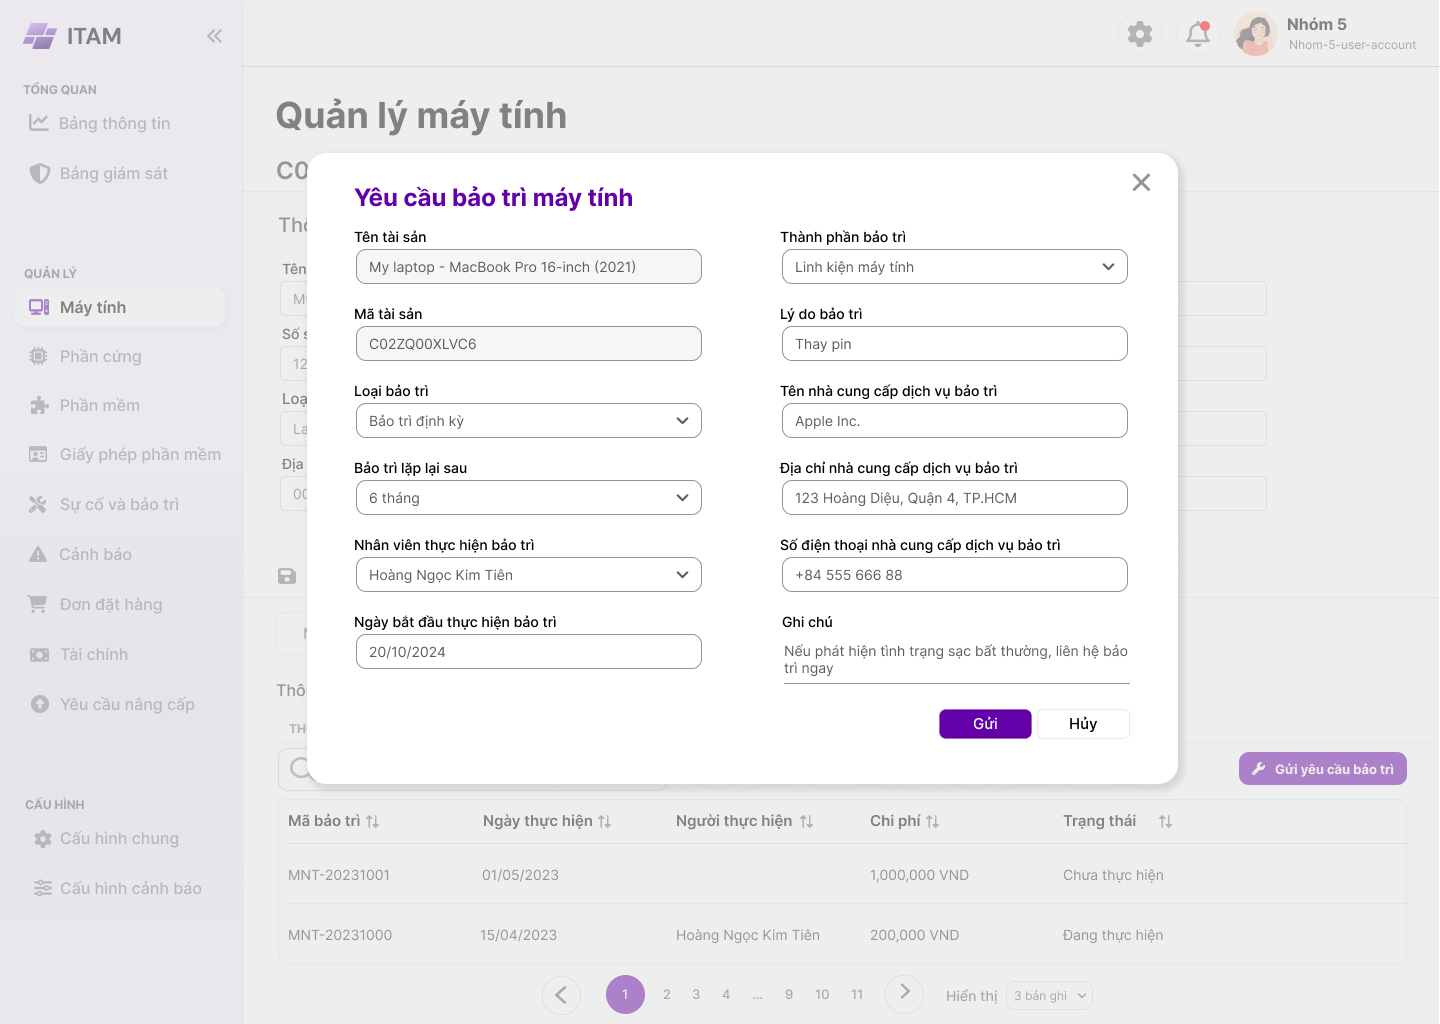
\includegraphics[width=14cm]{Images/C5/UI/Feature-Giám sát tài sản-Máy tính 6.12.png}
%     \vspace{15pt}
%     \caption{Giao diện Quản lý máy tính 11}
% \end{figure}
% \begin{figure}[H]
%     \centering
%     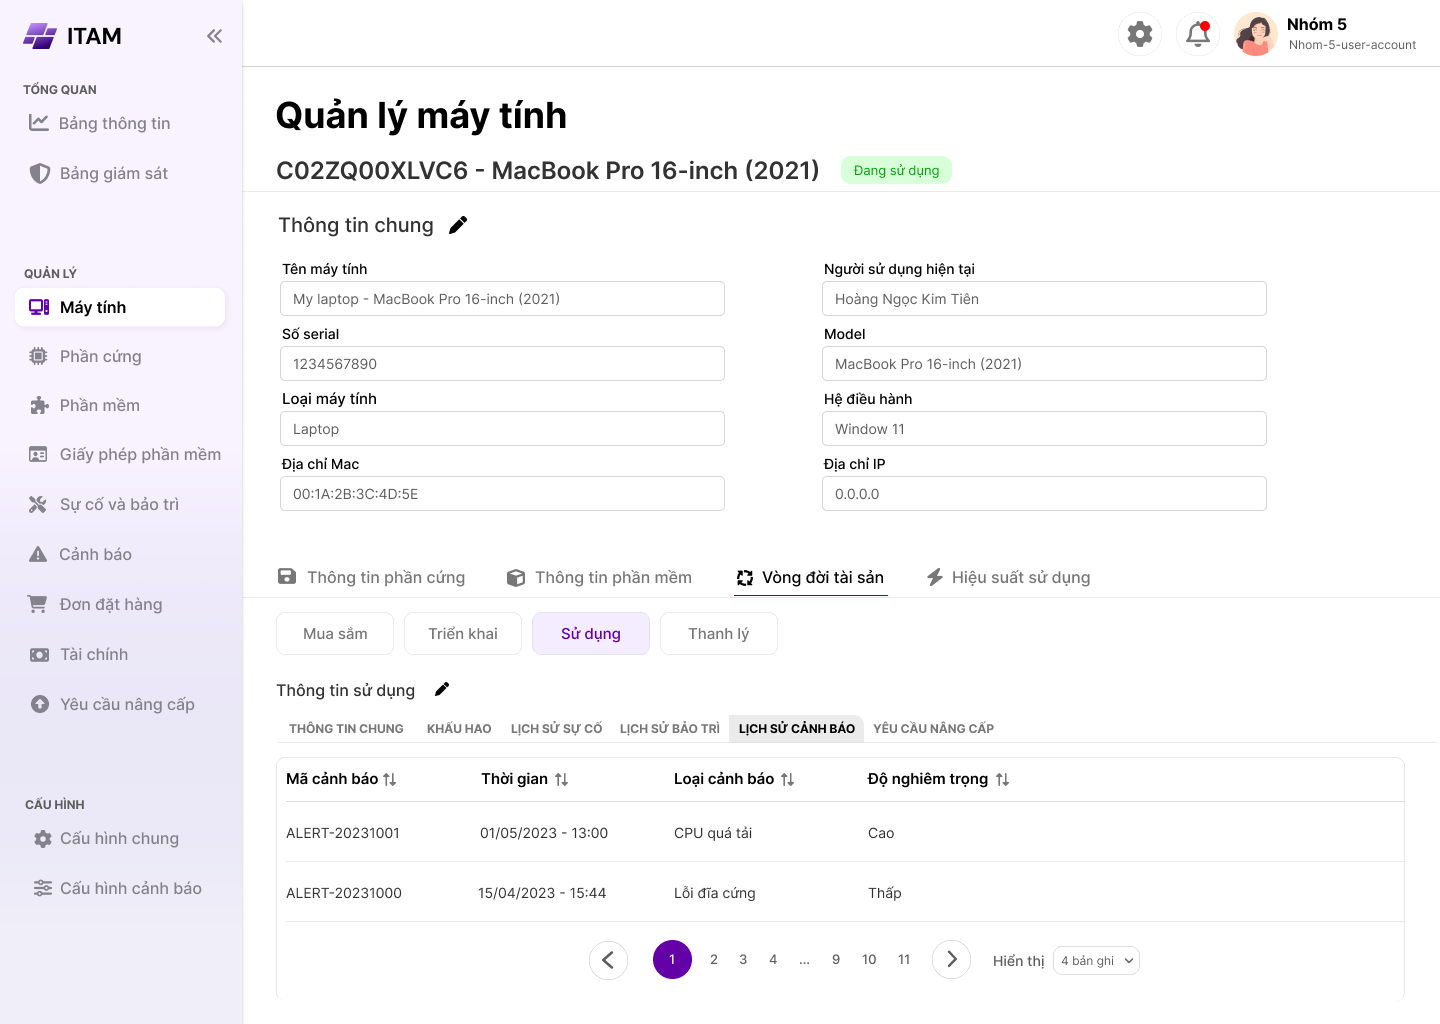
\includegraphics[width=14cm]{Images/C5/UI/Feature-Giám sát tài sản-Máy tính 6.13.png}
%     \vspace{15pt}
%     \caption{Giao diện Quản lý máy tính 15}
% \end{figure}
% \begin{figure}[H]
%     \centering
%     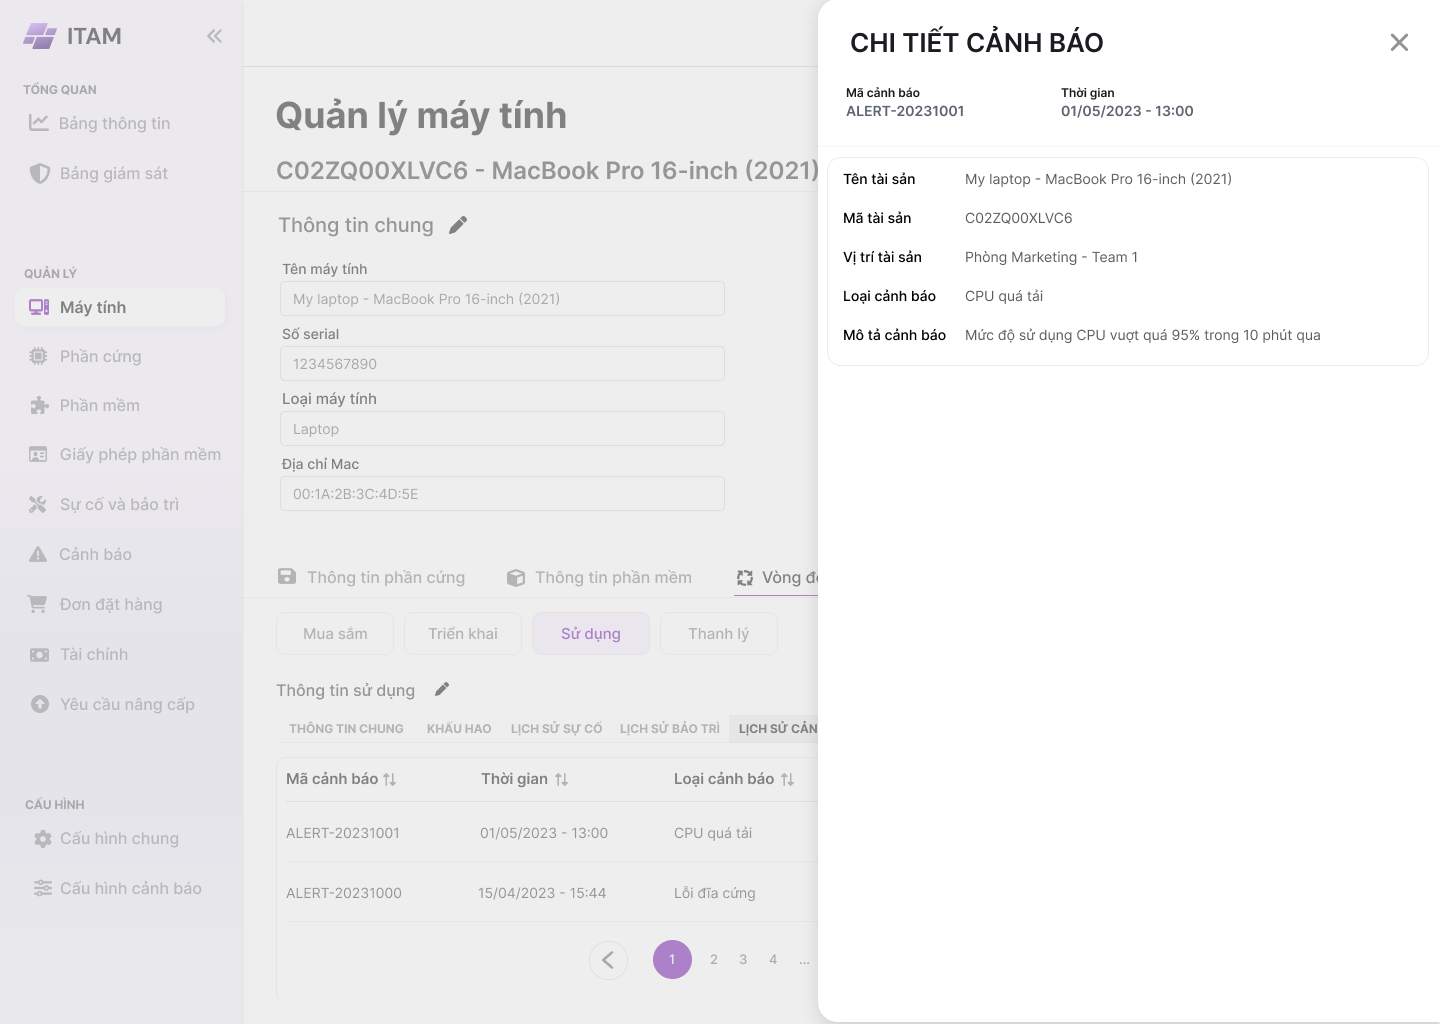
\includegraphics[width=14cm]{Images/C5/UI/Feature-Giám sát tài sản-Máy tính 6.14.png}
%     \vspace{15pt}
%     \caption{Giao diện Quản lý máy tính 22}
% \end{figure}
% \begin{figure}[H]
%     \centering
%     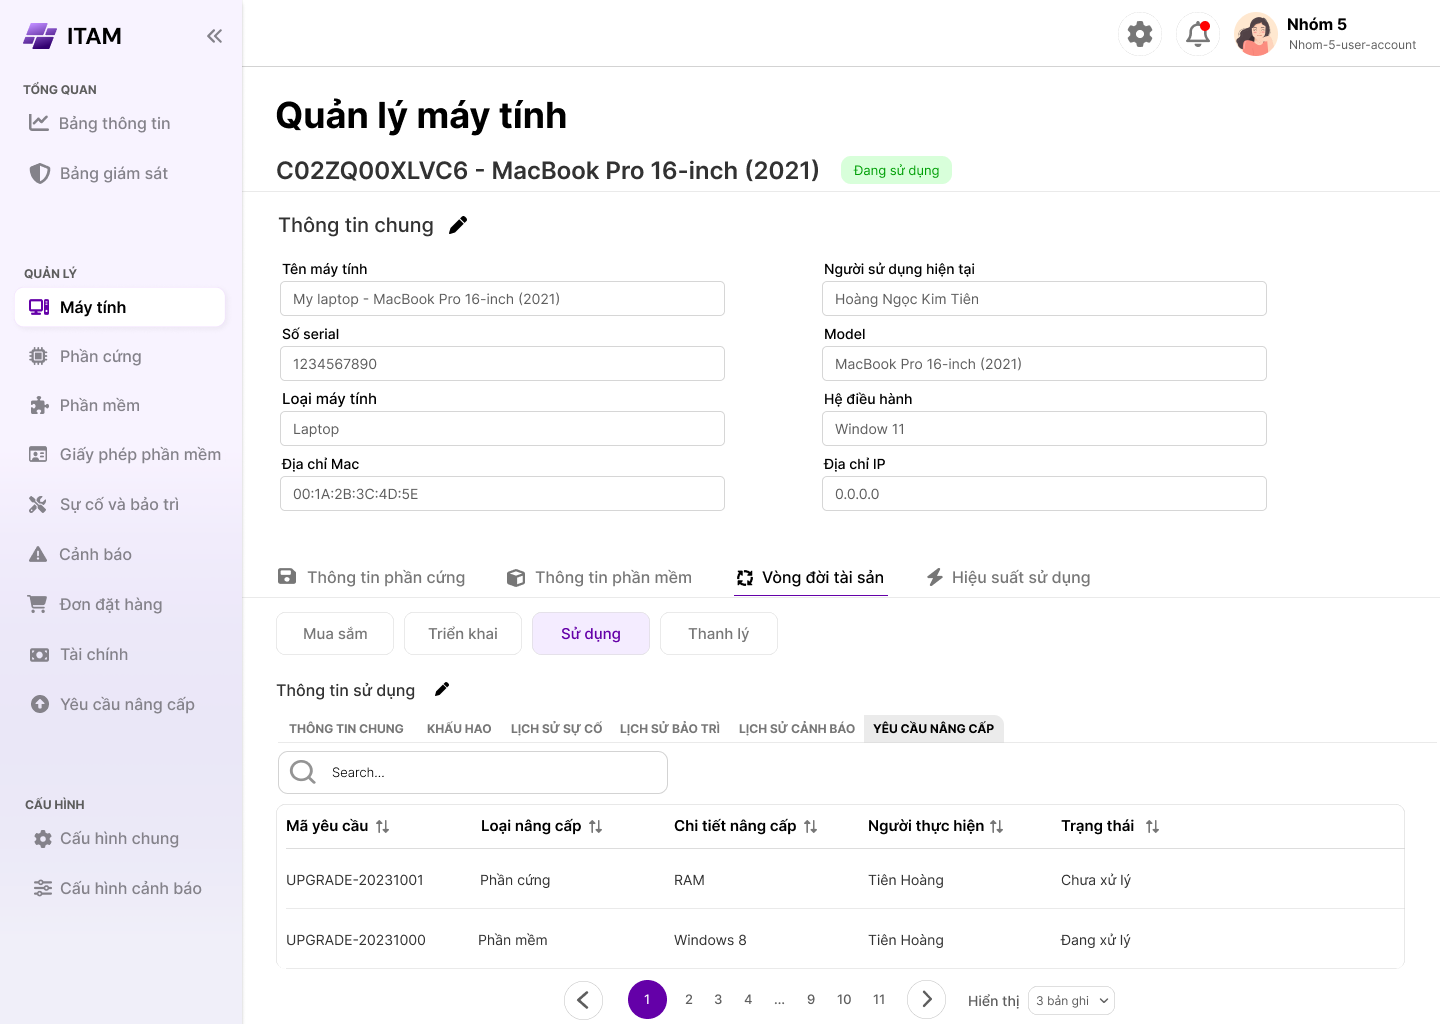
\includegraphics[width=14cm]{Images/C5/UI/Feature-Giám sát tài sản-Máy tính 6.15.png}
%     \vspace{15pt}
%     \caption{Giao diện Quản lý máy tính 16}
% \end{figure}
% \begin{figure}[H]
%     \centering
%     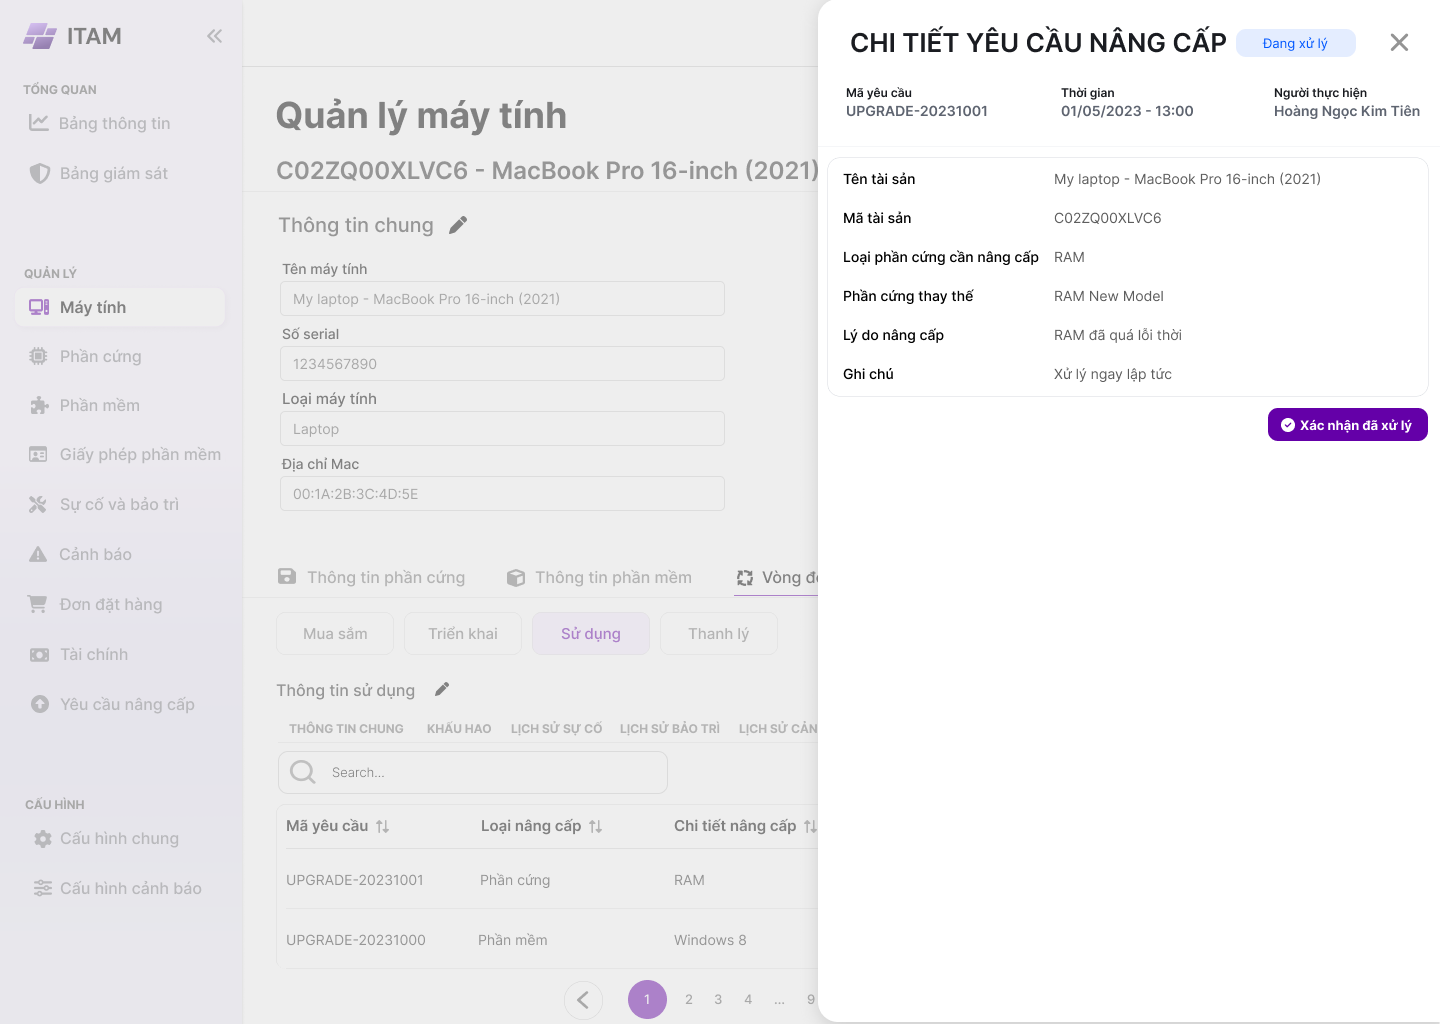
\includegraphics[width=14cm]{Images/C5/UI/Feature-Giám sát tài sản-Máy tính 6.16.png}
%     \vspace{15pt}
%     \caption{Giao diện Quản lý máy tính 24}
% \end{figure}
% \begin{figure}[H]
%     \centering
%     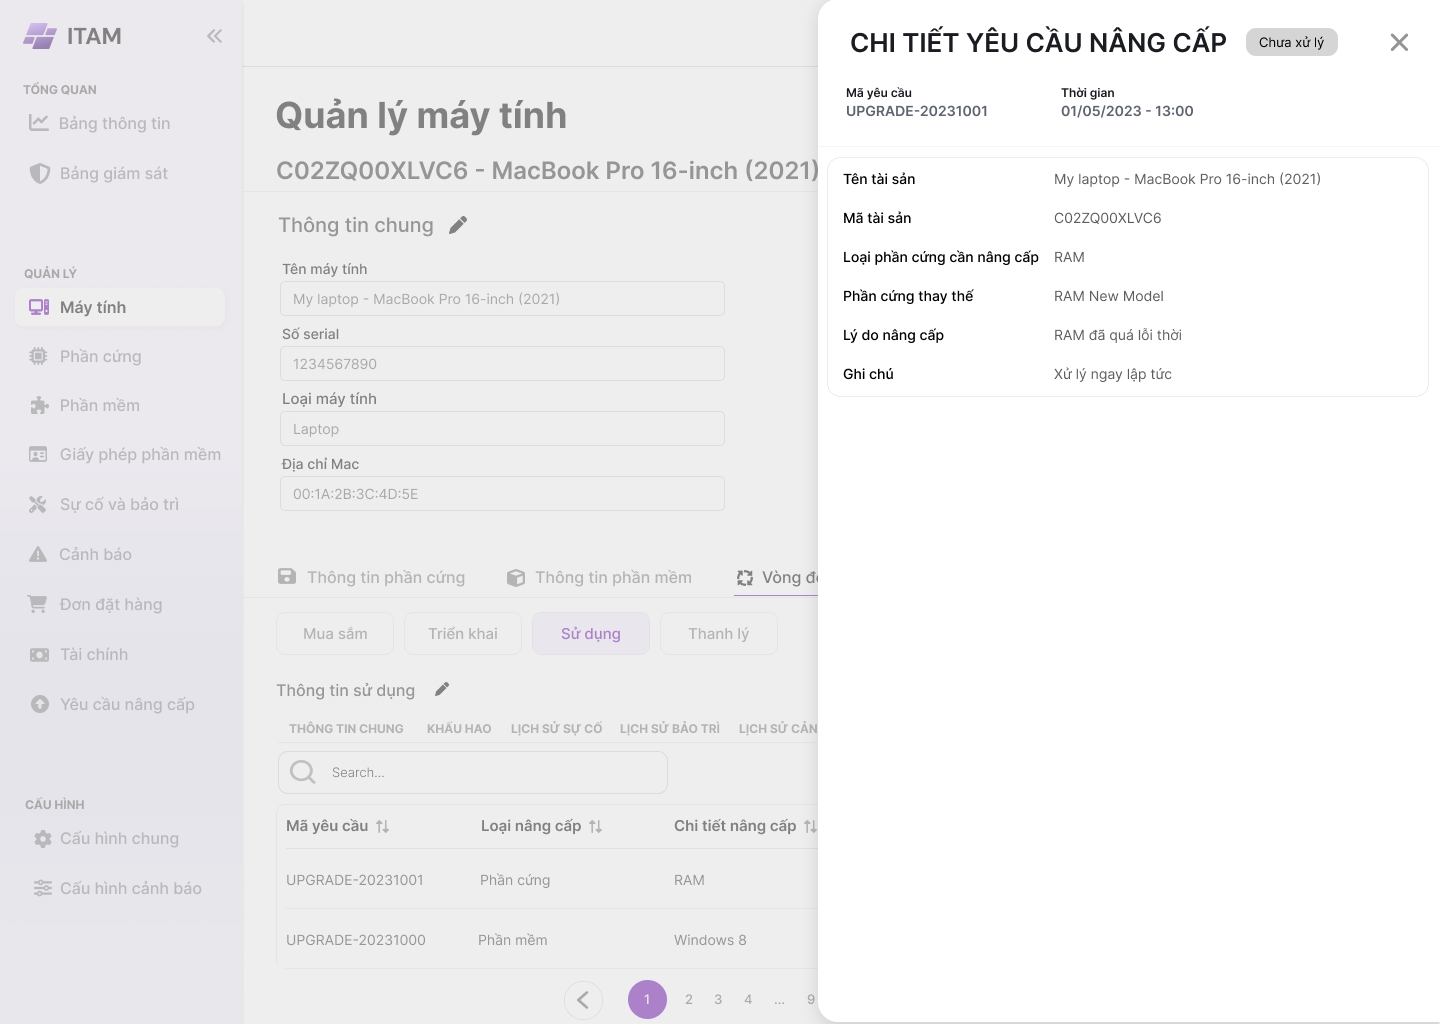
\includegraphics[width=14cm]{Images/C5/UI/Feature-Giám sát tài sản-Máy tính 6.17.png}
%     \vspace{15pt}
%     \caption{Giao diện Quản lý máy tính 25}
% \end{figure}
% \begin{figure}[H]
%     \centering
%     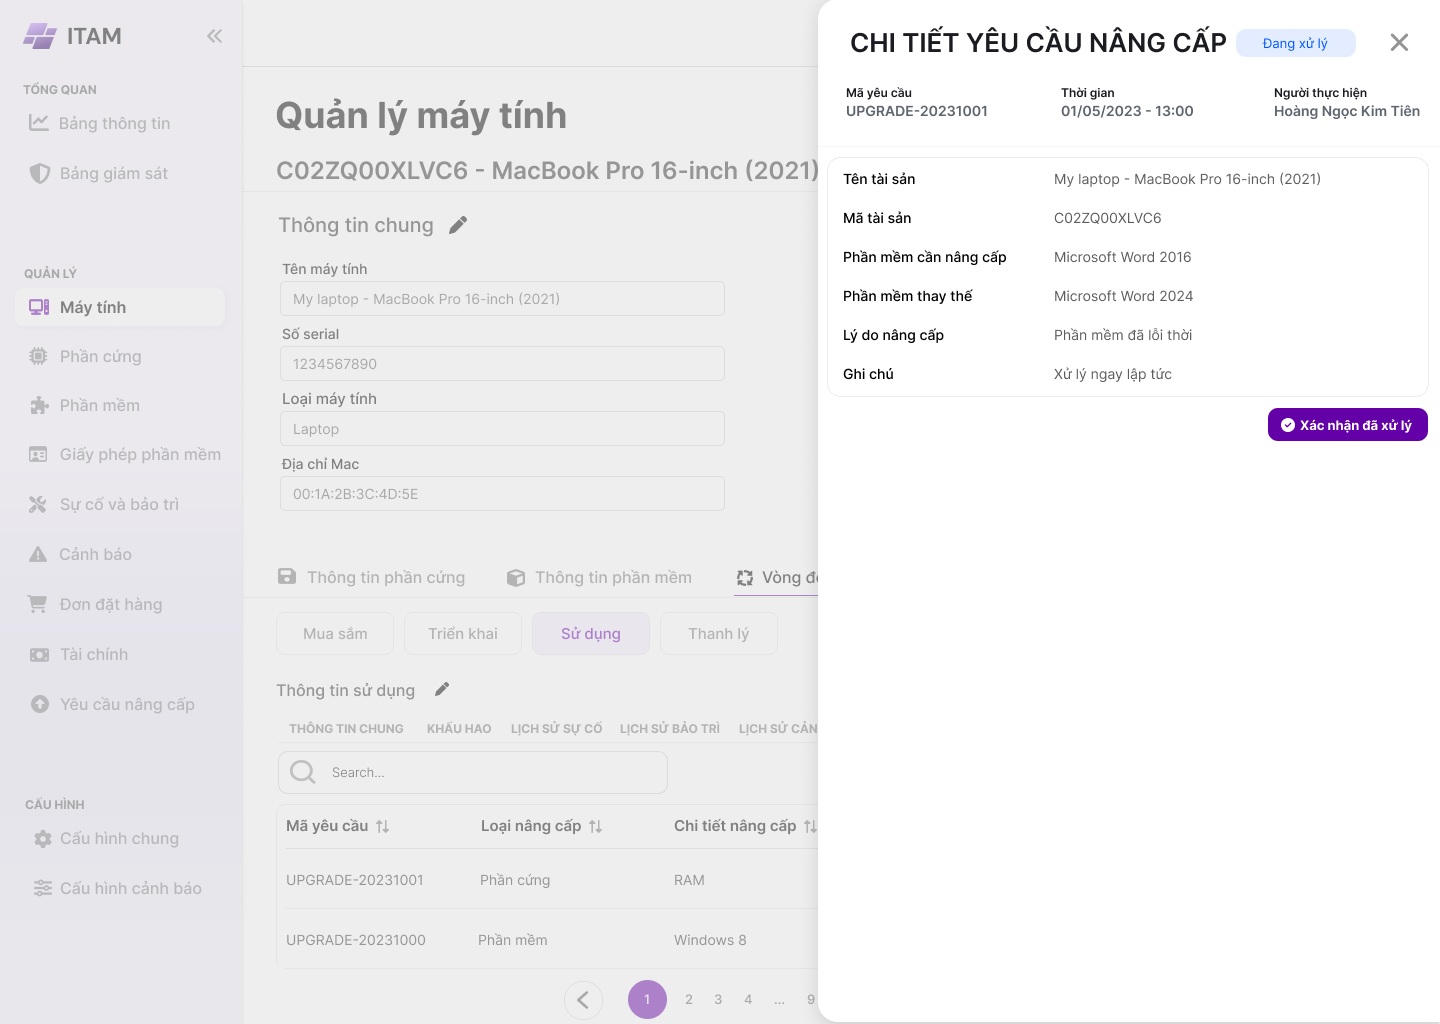
\includegraphics[width=14cm]{Images/C5/UI/Feature-Giám sát tài sản-Máy tính 6.18.png}
%     \vspace{15pt}
%     \caption{Giao diện Quản lý máy tính 26}
% \end{figure}
% \begin{figure}[H]
%     \centering
%     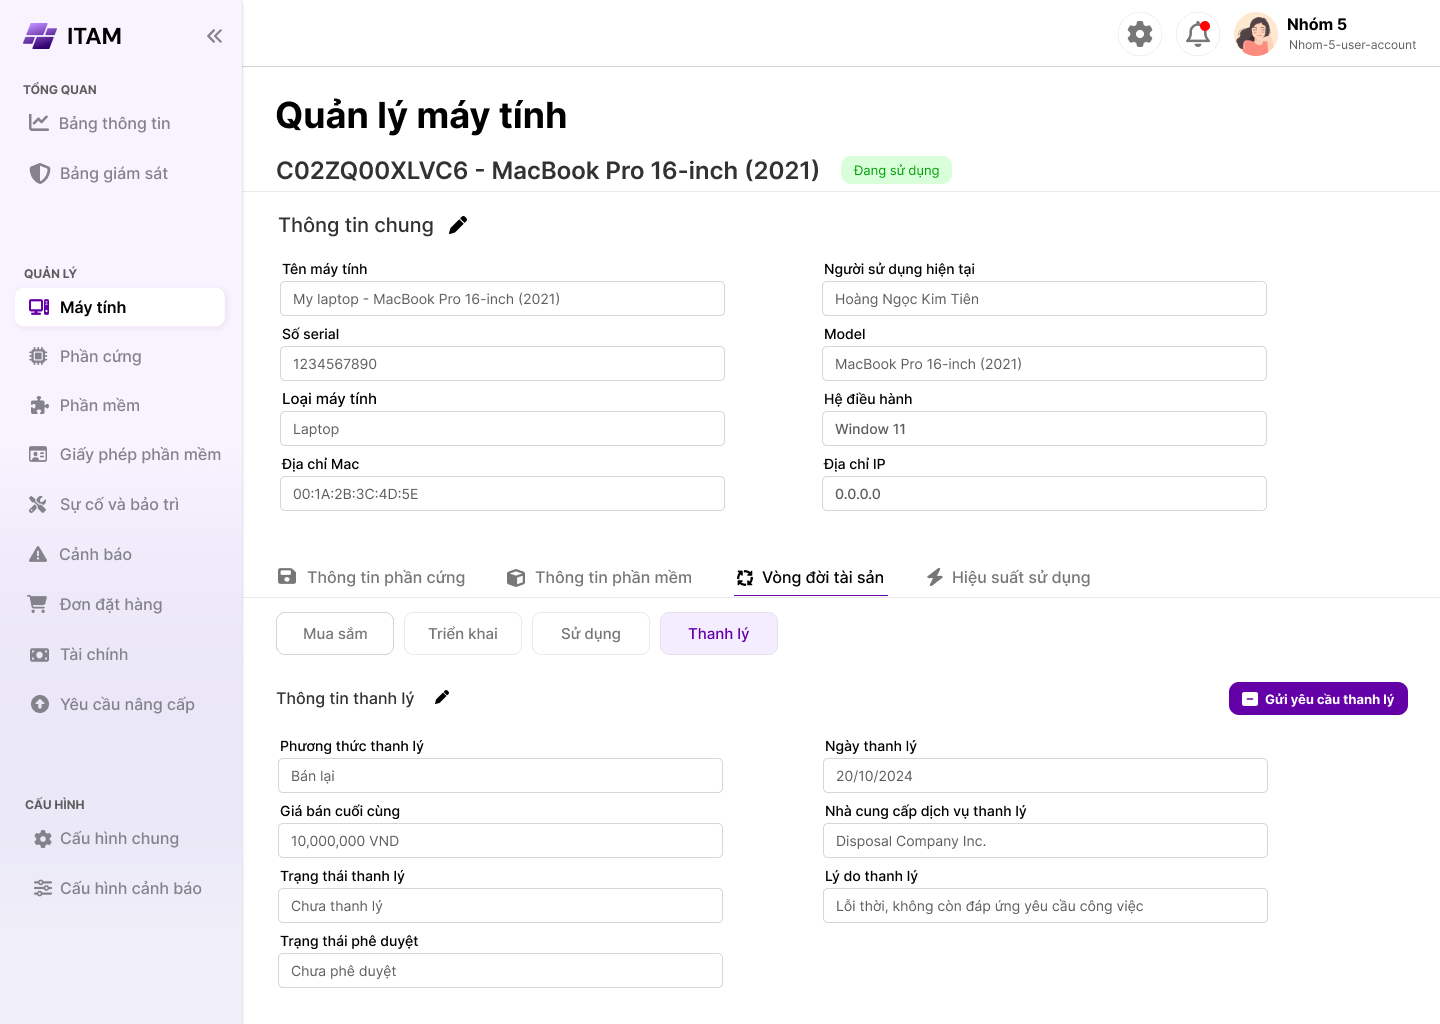
\includegraphics[width=14cm]{Images/C5/UI/Feature-Giám sát tài sản-Máy tính 7.1.png}
%     \vspace{15pt}
%     \caption{Giao diện Quản lý máy tính 12}
% \end{figure}
% \begin{figure}[H]
%     \centering
%     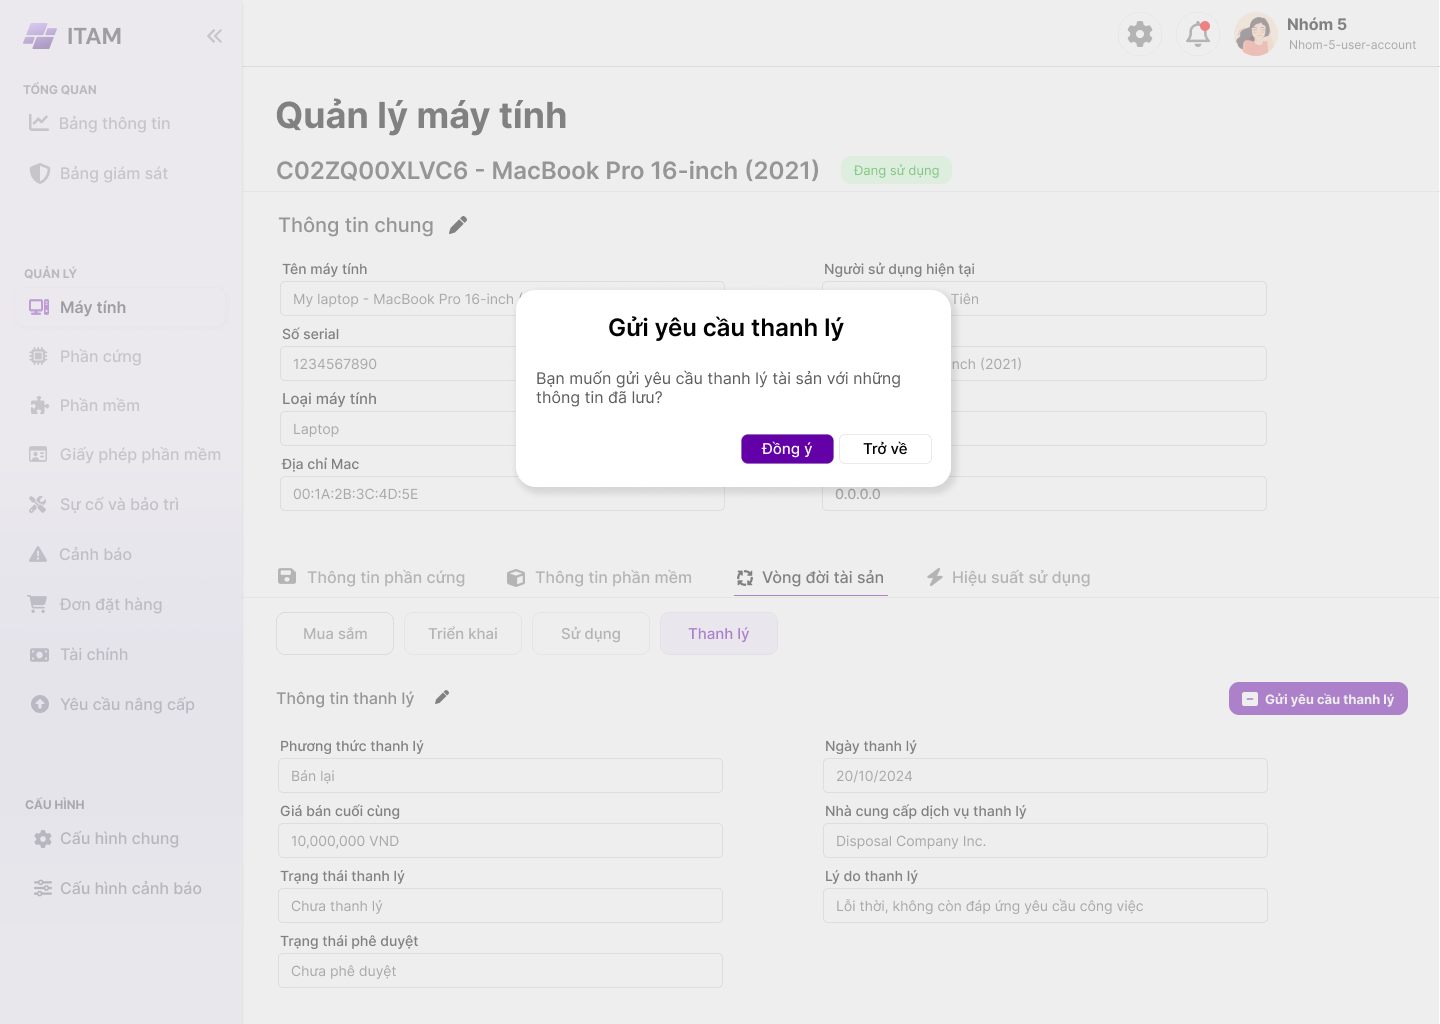
\includegraphics[width=14cm]{Images/C5/UI/Feature-Giám sát tài sản-Máy tính 7.2.png}
%     \vspace{15pt}
%     \caption{Giao diện Quản lý máy tính 28}
% \end{figure}
% \begin{figure}[H]
%     \centering
%     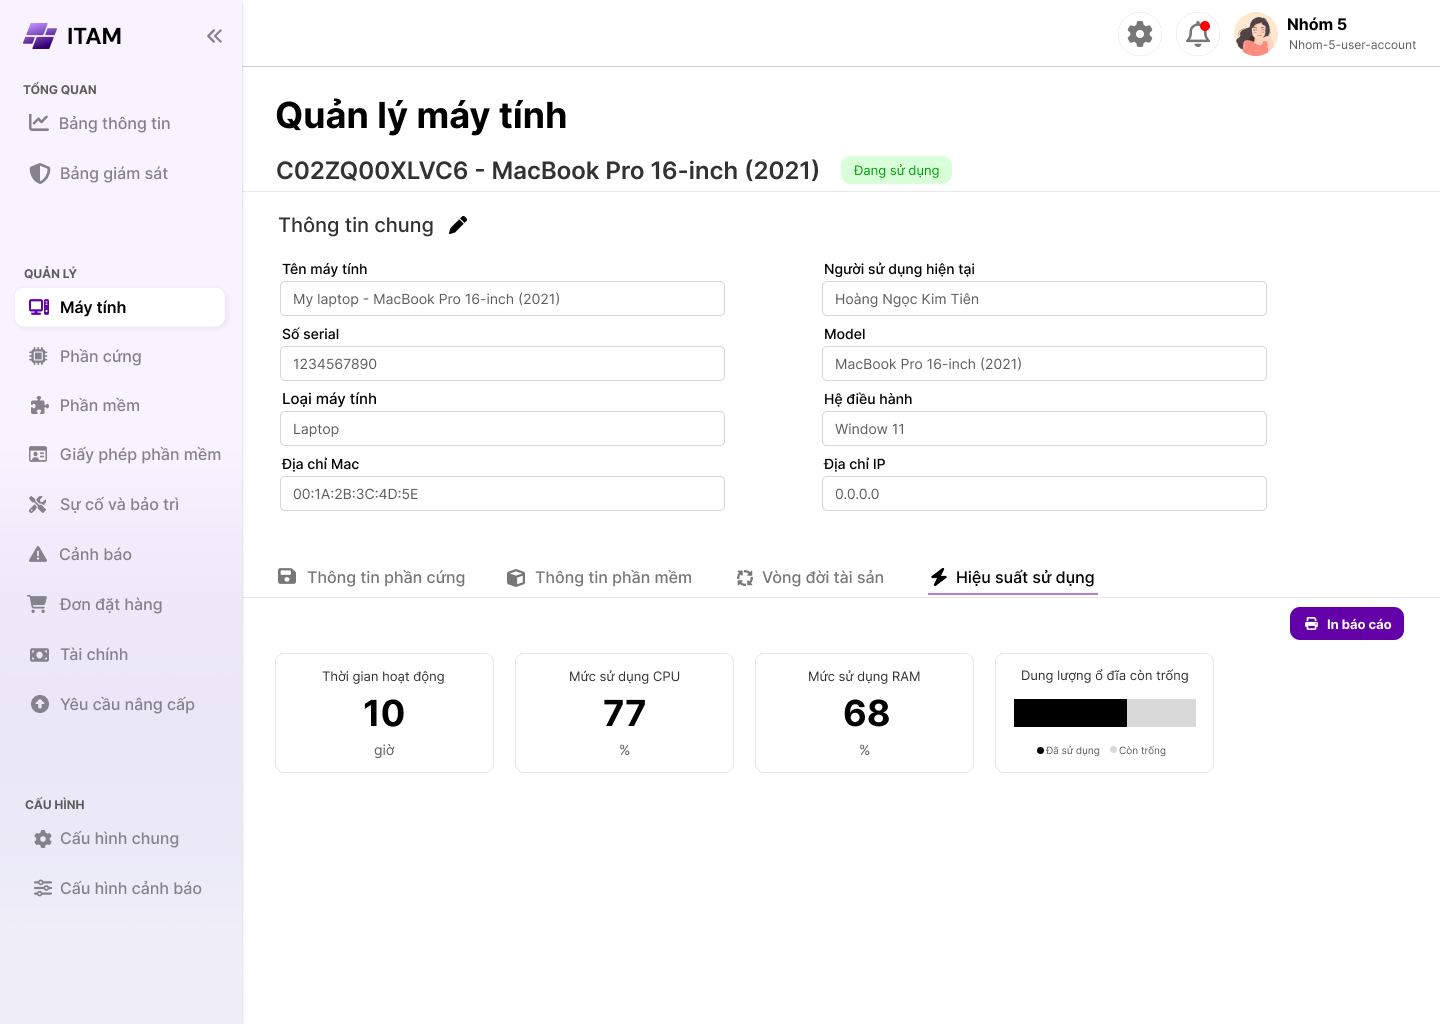
\includegraphics[width=14cm]{Images/C5/UI/Feature-Giám sát tài sản-Máy tính 9.1.png}
%     \vspace{15pt}
%     \caption{Giao diện Quản lý máy tính 2}
% \end{figure}
\begin{figure}[H]
    \centering
    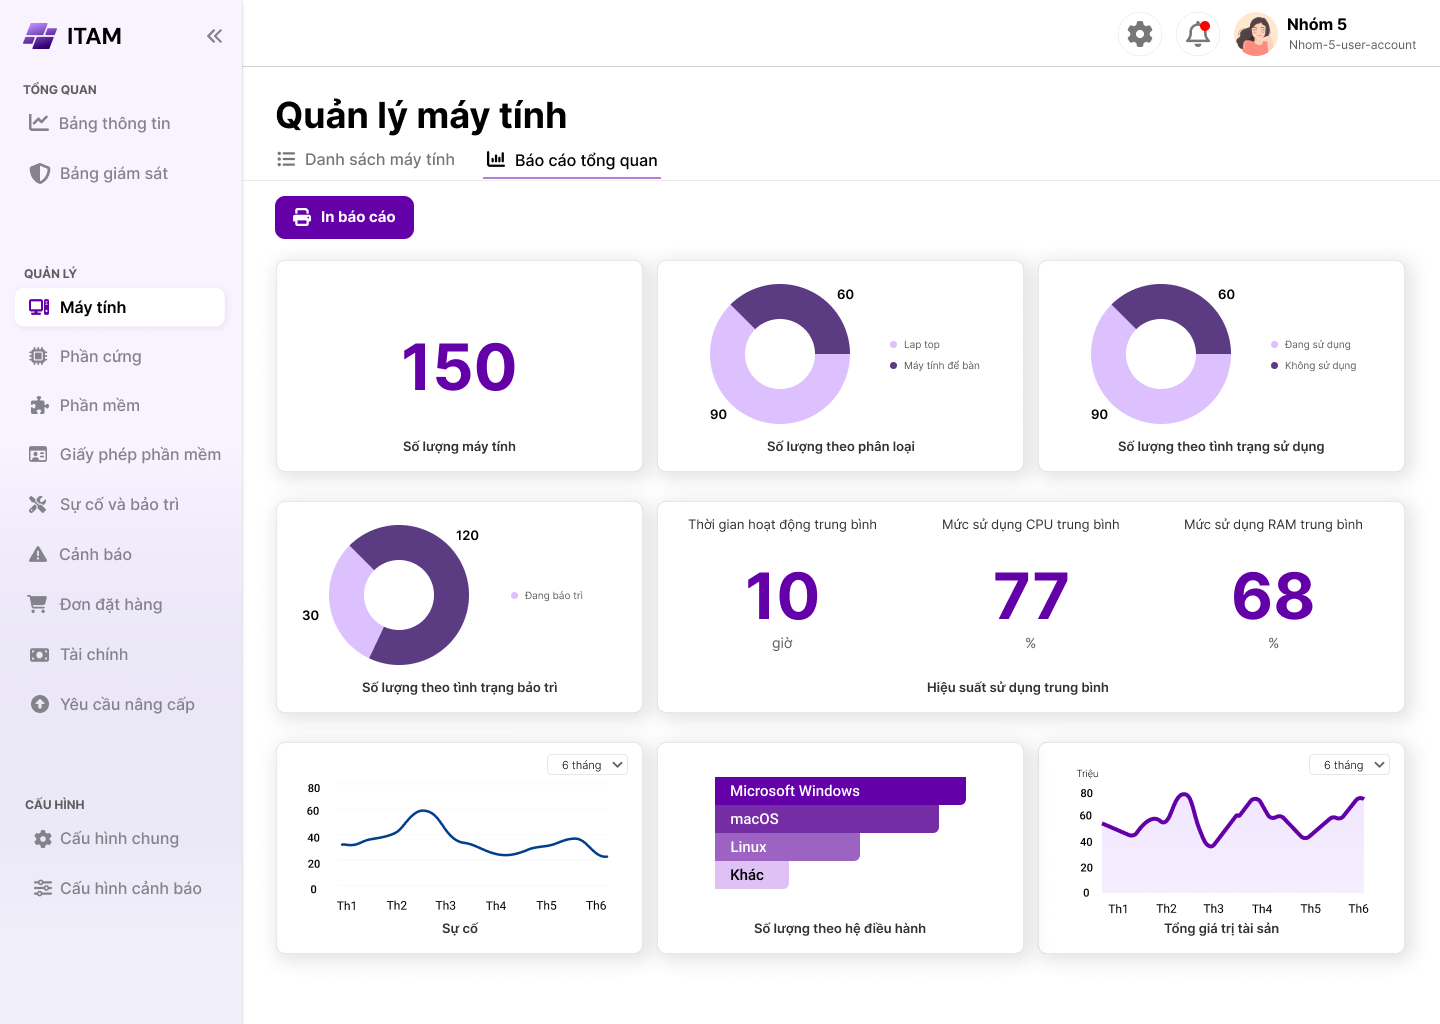
\includegraphics[width=14cm]{Images/C5/UI/Feature-Giám sát tài sản-Máy tính 10.png}
    \vspace{15pt}
    \caption{Giao diện Quản lý máy tính 2}
\end{figure}

\item{Quản lý phần cứng}\\
Ở chức năng Quản lý phần cứng, người dùng có thể dễ dàng xem danh sách tất cả các phần cứng trong hệ thống, thêm mới phần cứng, xem chi tiết phần cứng, gửi yêu cầu bảo trì cho phần cứng, và xem báo cáo tổng quan về phần cứng (xem thêm chi tiết ở phụ lục).
% \begin{figure}[H]
%     \centering
%     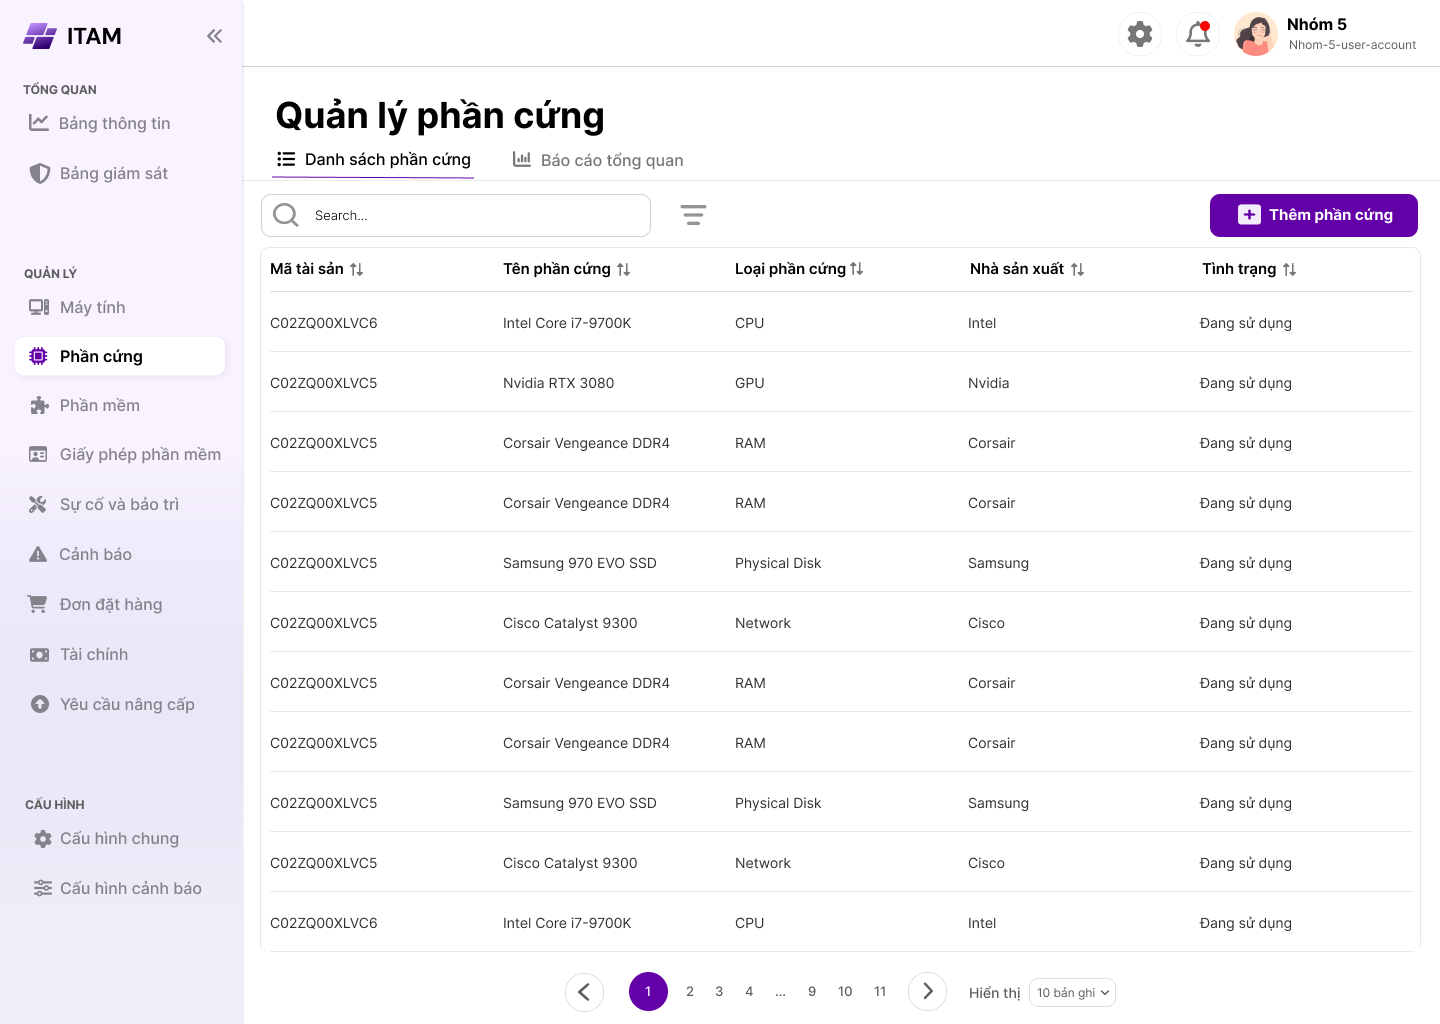
\includegraphics[width=14cm]{Images/C5/UI/Feature-Giám sát tài sản-Phần cứng 1.png}
%     \vspace{15pt}
%     \caption{Giao diện Quản lý phần cứng 1}
% \end{figure}
% \begin{figure}[H]
%     \centering
%     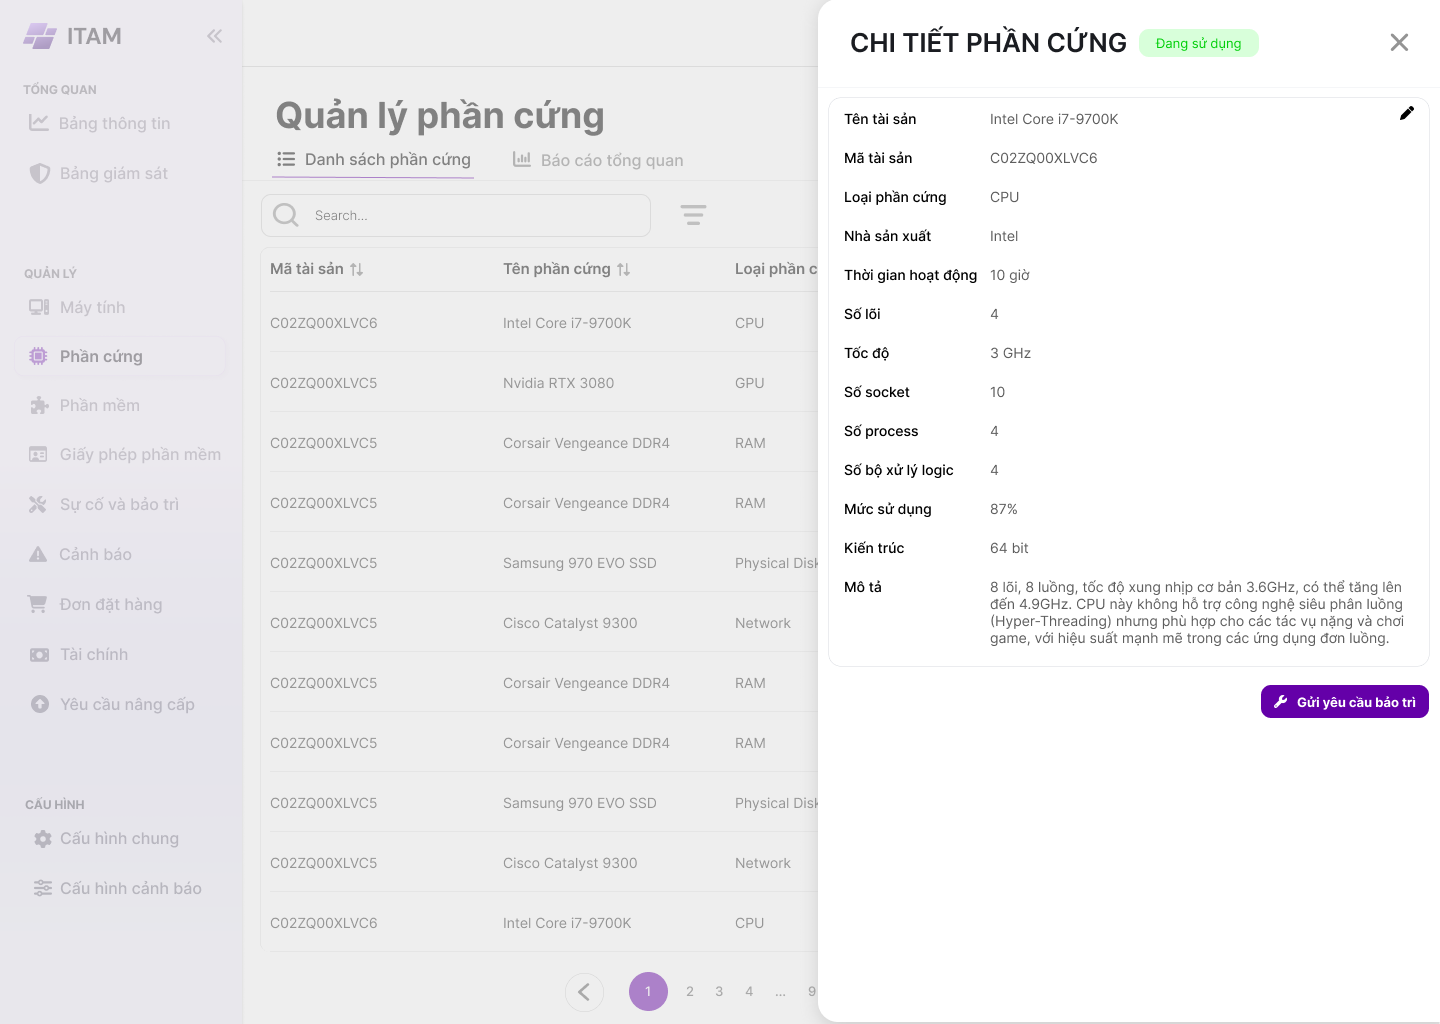
\includegraphics[width=14cm]{Images/C5/UI/Feature-Giám sát tài sản-Phần cứng 2.1-CPU.png}
%     \vspace{15pt}
%     \caption{Giao diện Quản lý phần cứng 2}
% \end{figure}
% \begin{figure}[H]
%     \centering
%     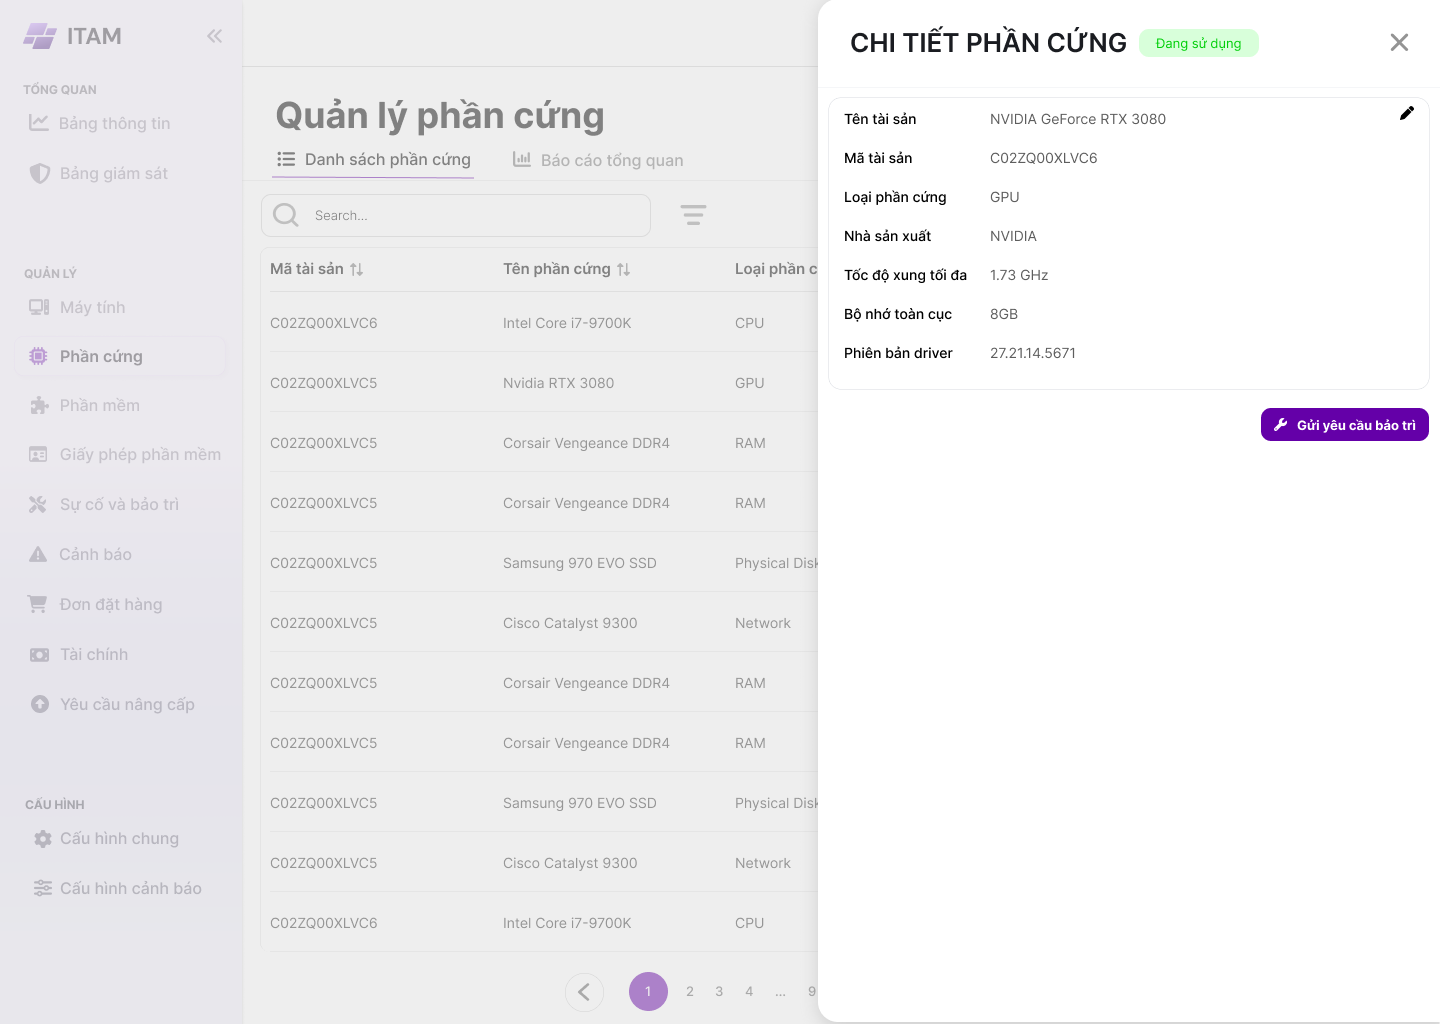
\includegraphics[width=14cm]{Images/C5/UI/Feature-Giám sát tài sản-Phần cứng 2.2-GPU.png}
%     \vspace{15pt}
%     \caption{Giao diện Quản lý phần cứng 3}
% \end{figure}
% \begin{figure}[H]
%     \centering
%     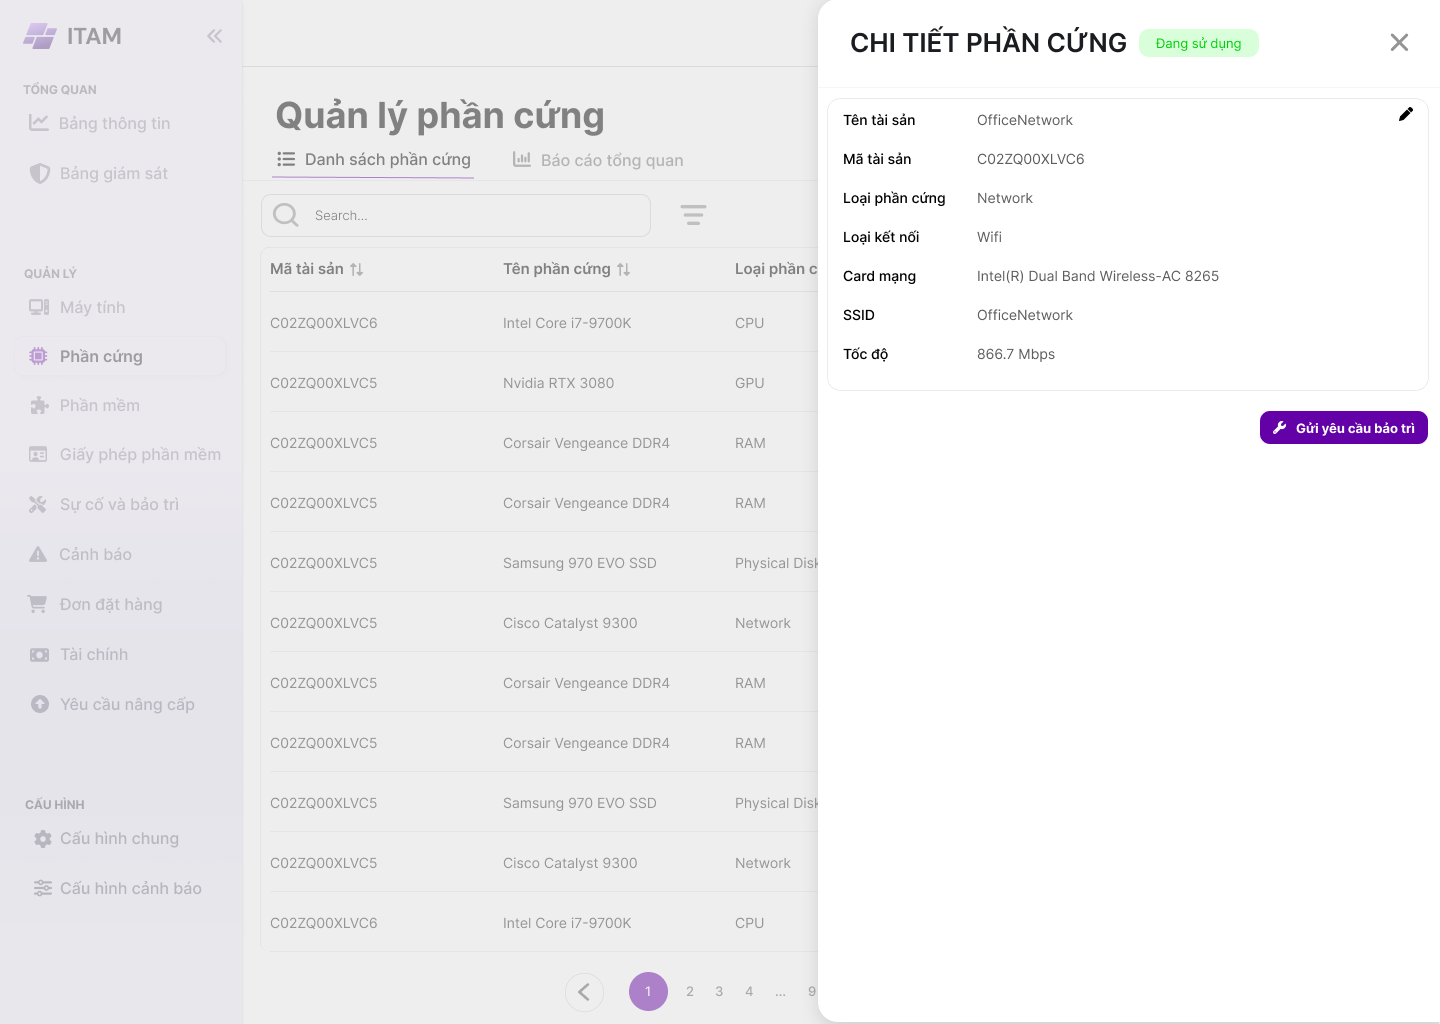
\includegraphics[width=14cm]{Images/C5/UI/Feature-Giám sát tài sản-Phần cứng 2.3-Network.png}
%     \vspace{15pt}
%     \caption{Giao diện Quản lý phần cứng 4}
% \end{figure}
% \begin{figure}[H]
%     \centering
%     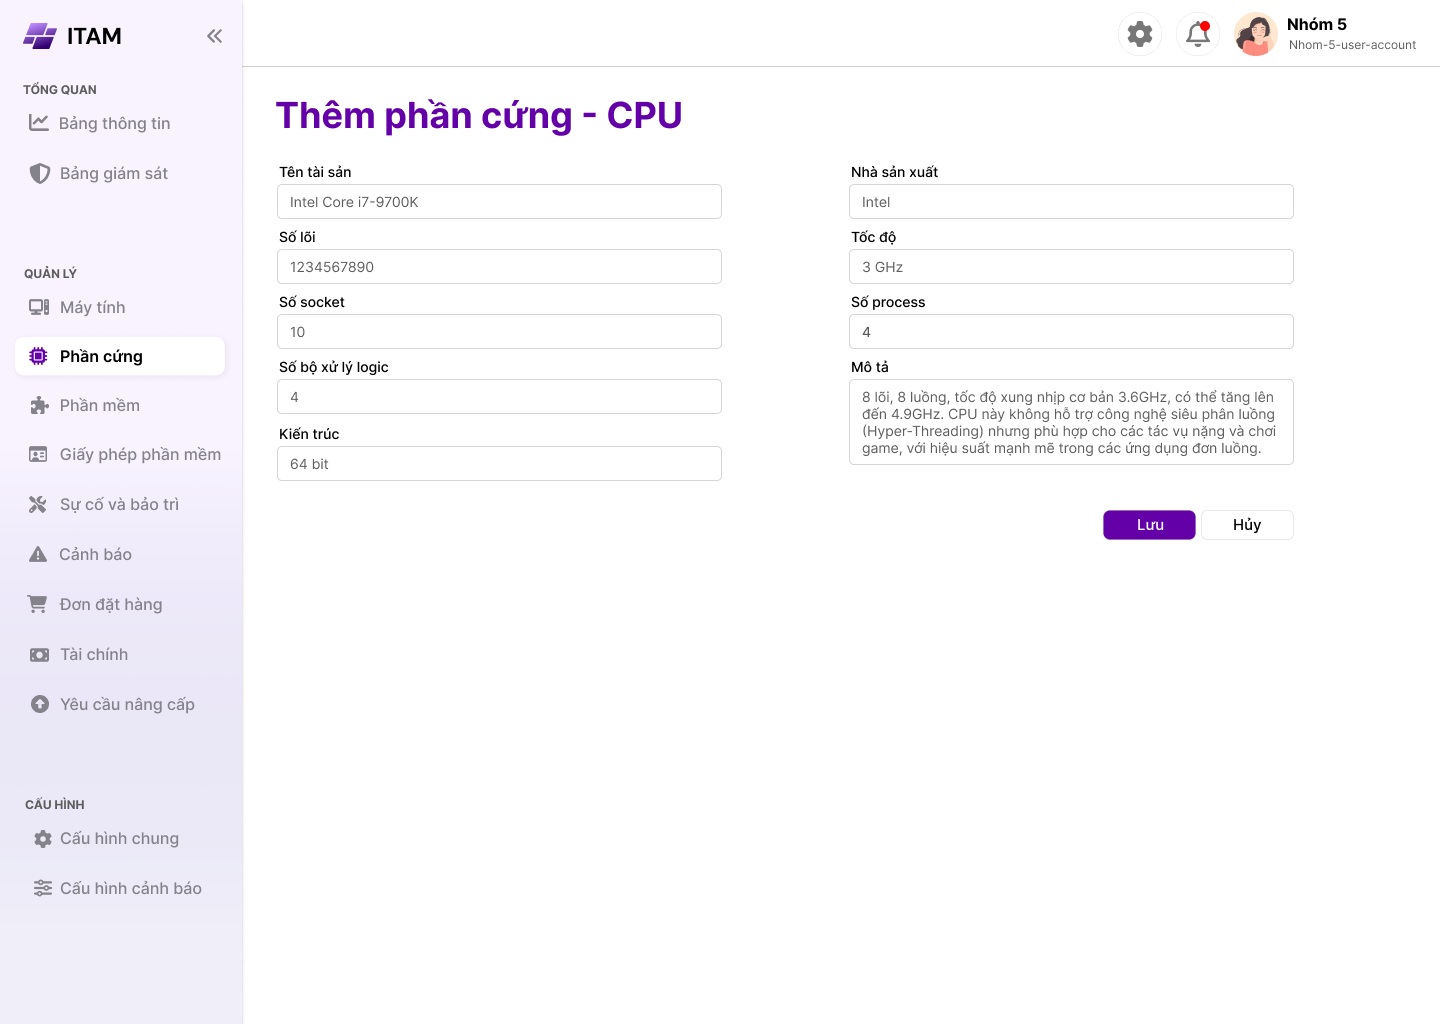
\includegraphics[width=14cm]{Images/C5/UI/Feature-Giám sát tài sản-Phần cứng 4.2.png}
%     \vspace{15pt}
%     \caption{Giao diện Quản lý phần cứng 3}
% \end{figure}
% \begin{figure}[H]
%     \centering
%     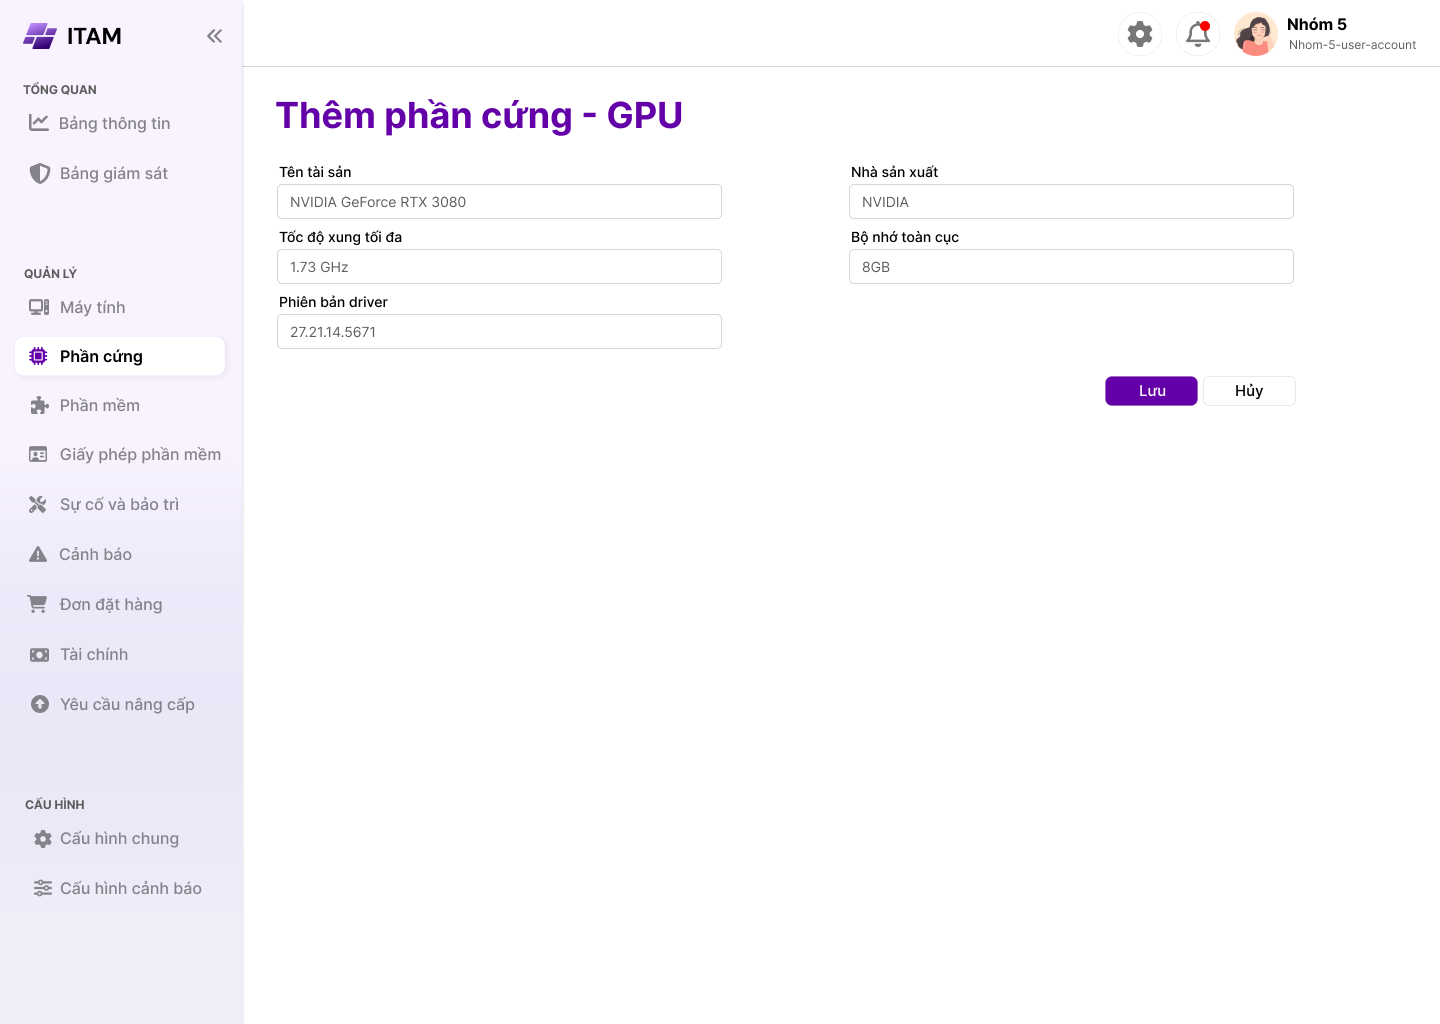
\includegraphics[width=14cm]{Images/C5/UI/Feature-Giám sát tài sản-Phần cứng 4.3.png}
%     \vspace{15pt}
%     \caption{Giao diện Quản lý phần cứng 6}
% \end{figure}
% \begin{figure}[H]
%     \centering
%     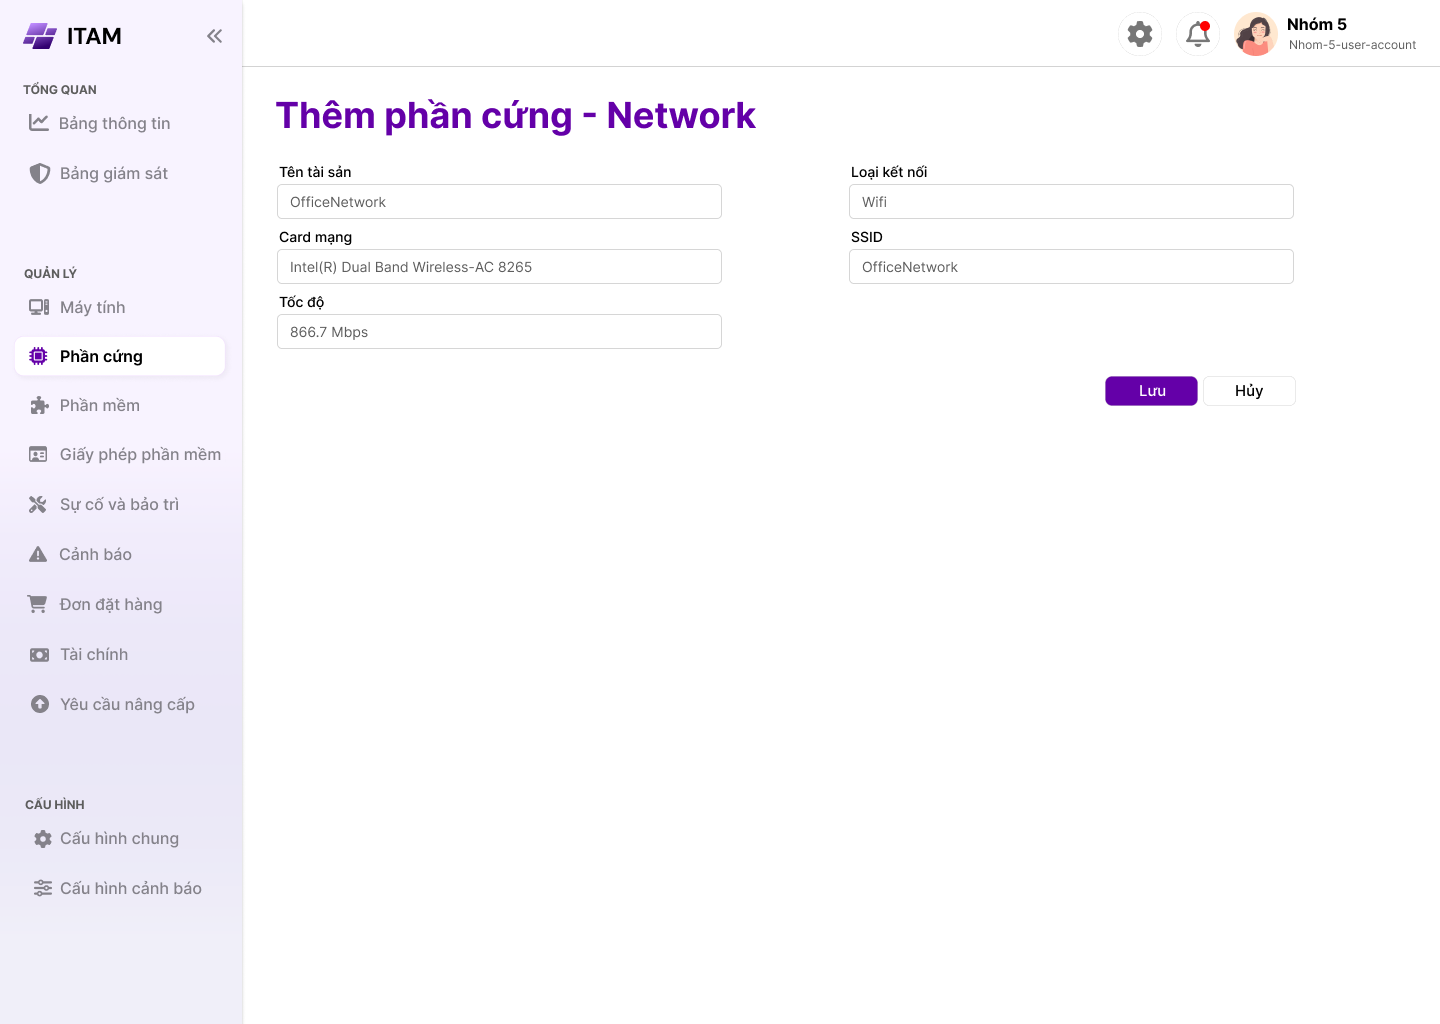
\includegraphics[width=14cm]{Images/C5/UI/Feature-Giám sát tài sản-Phần cứng 4.4.png}
%     \vspace{15pt}
%     \caption{Giao diện Quản lý phần cứng 7}
% \end{figure}
% \begin{figure}[H]
%     \centering
%     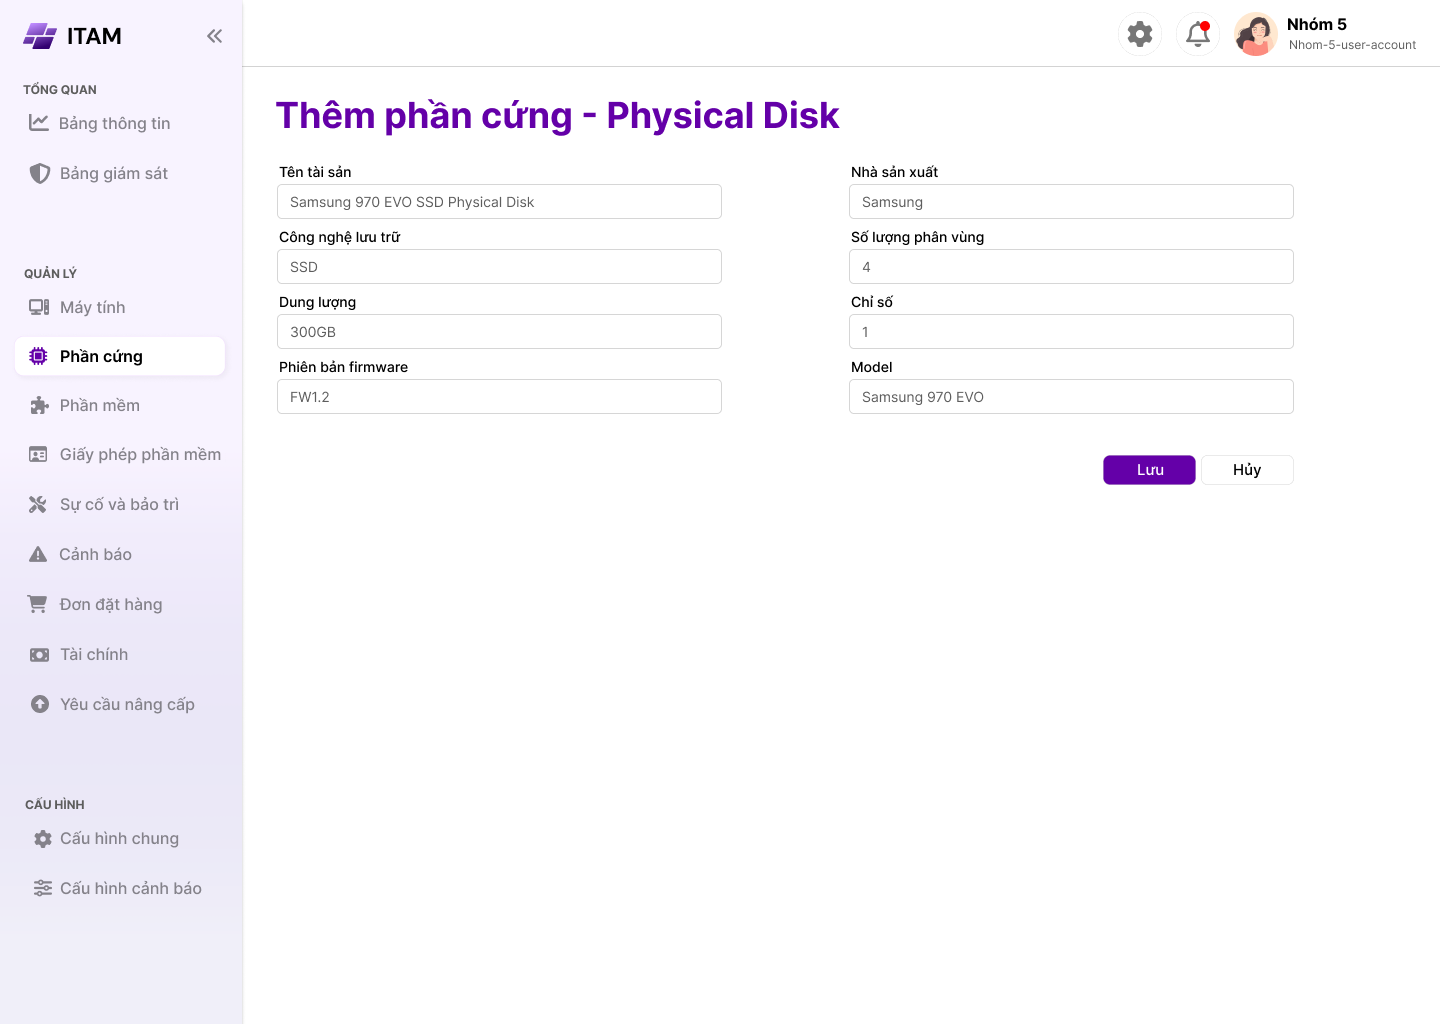
\includegraphics[width=14cm]{Images/C5/UI/Feature-Giám sát tài sản-Phần cứng 4.5.png}
%     \vspace{15pt}
%     \caption{Giao diện Quản lý phần cứng 8}
% \end{figure}
% \begin{figure}[H]
%     \centering
%     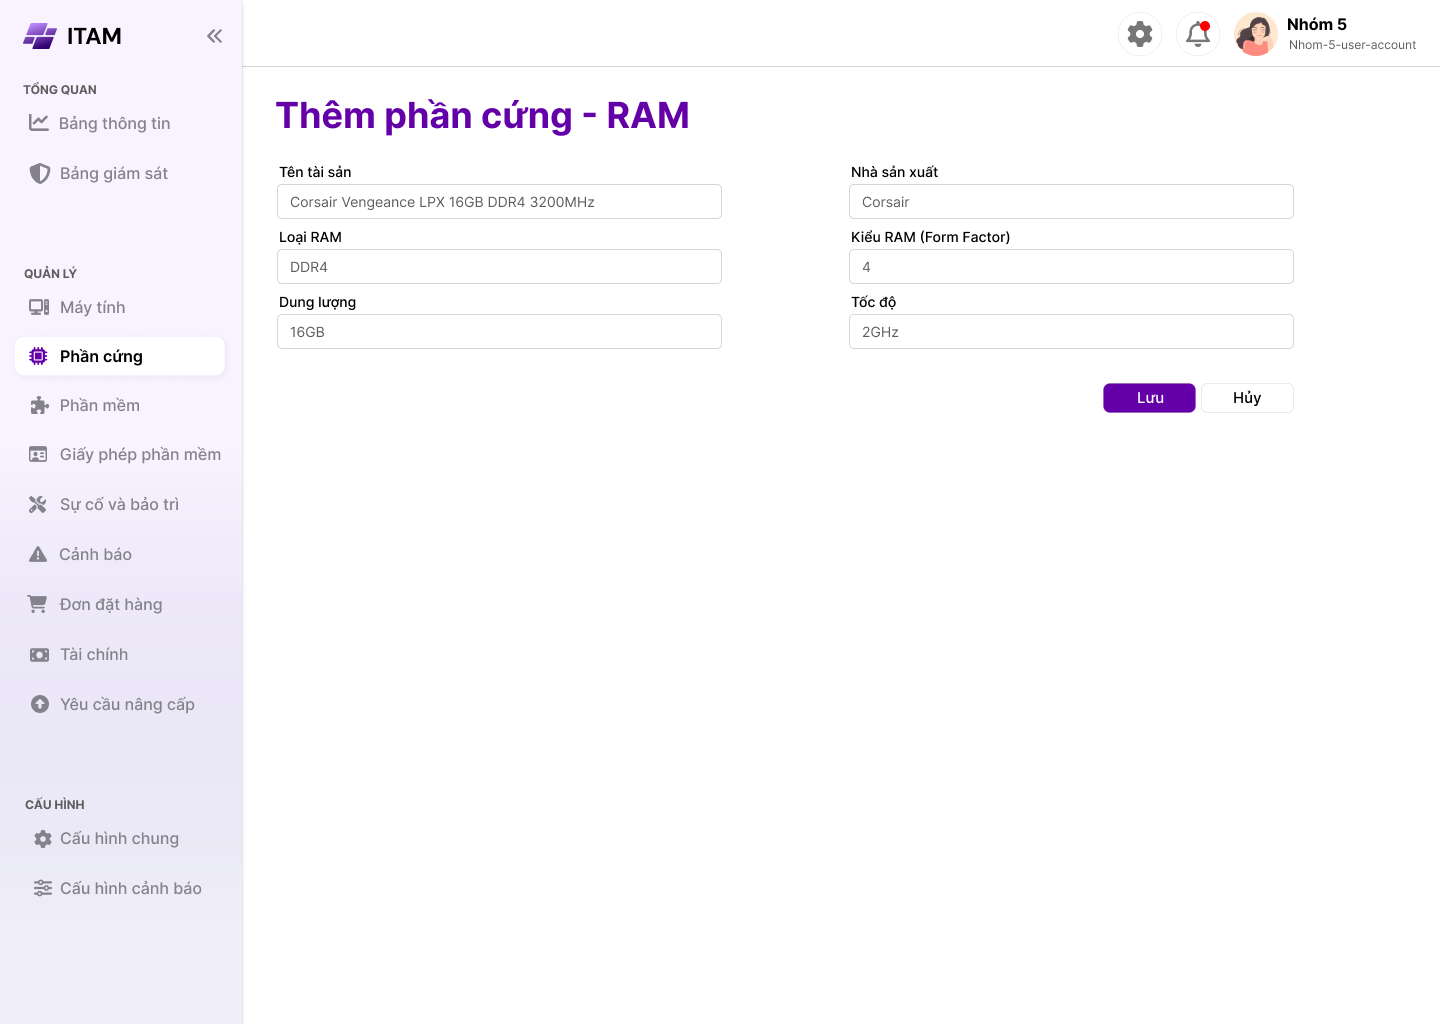
\includegraphics[width=14cm]{Images/C5/UI/Feature-Giám sát tài sản-Phần cứng 4.6.png}
%     \vspace{15pt}
%     \caption{Giao diện Quản lý phần cứng 9}
% \end{figure}
% \begin{figure}[H]
%     \centering
%     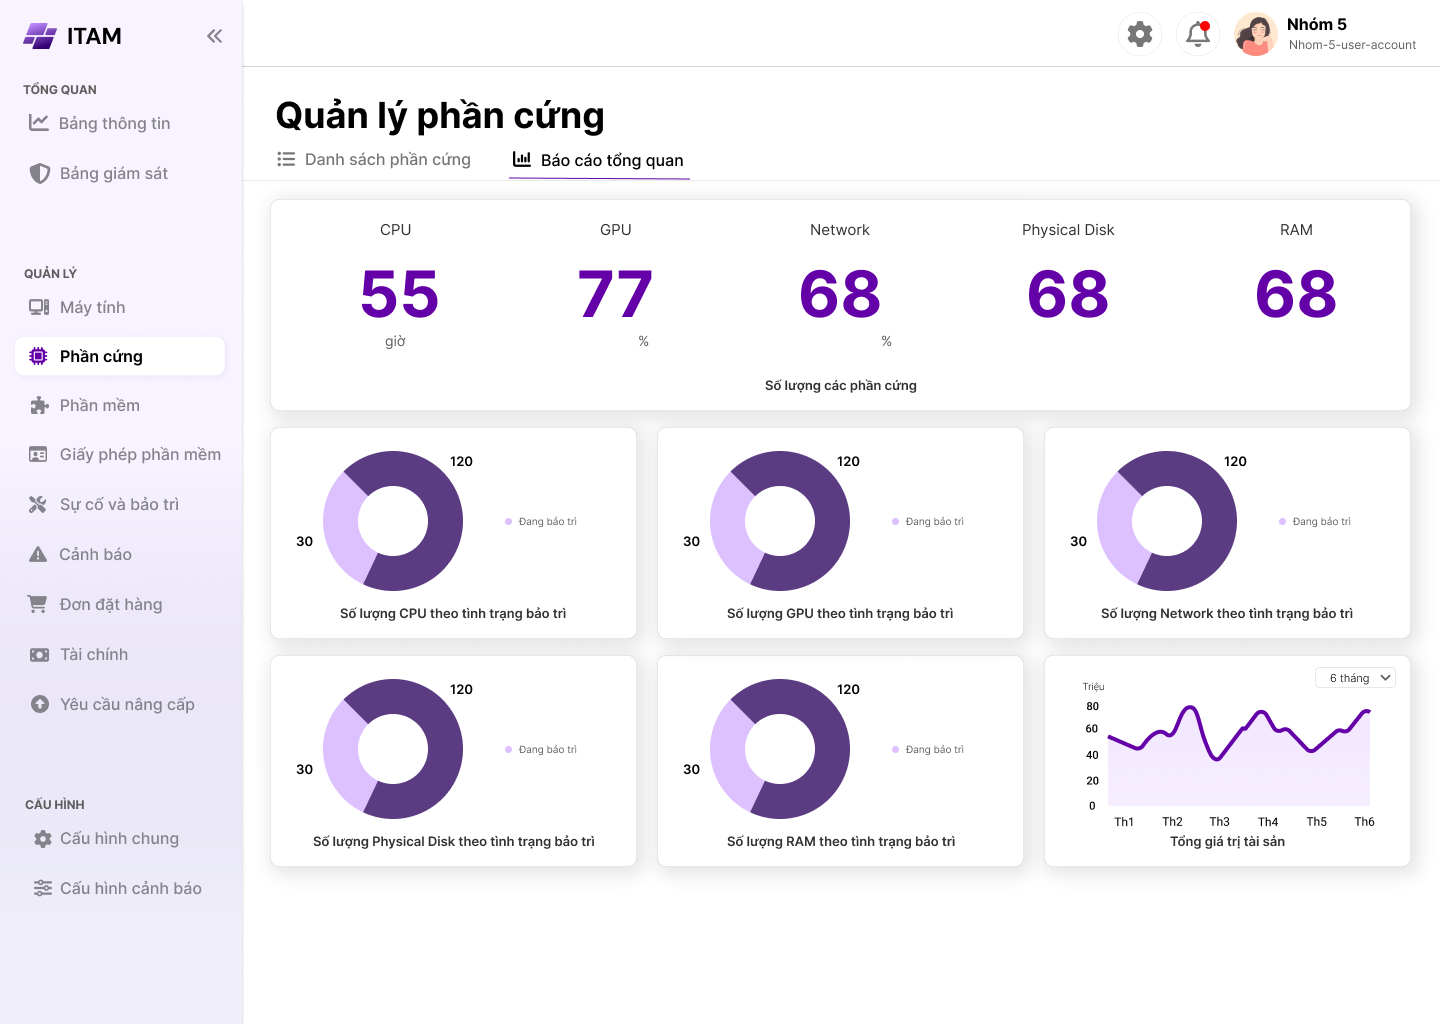
\includegraphics[width=14cm]{Images/C5/UI/Feature-Giám sát tài sản-Phần cứng 3.png}
%     \vspace{15pt}
%     \caption{Giao diện Quản lý phần cứng 4}
% \end{figure}

\item{Quản lý phần mềm}\\
Ở chức năng Quản lý phần mềm, người dùng có thể dễ dàng xem danh sách tất cả các phần mềm trong hệ thống, thêm mới phần mềm, xem chi tiết phần mềm, và xem báo cáo tổng quan về phần mềm (xem thêm chi tiết ở phụ lục).
% \begin{figure}[H]
%     \centering
%     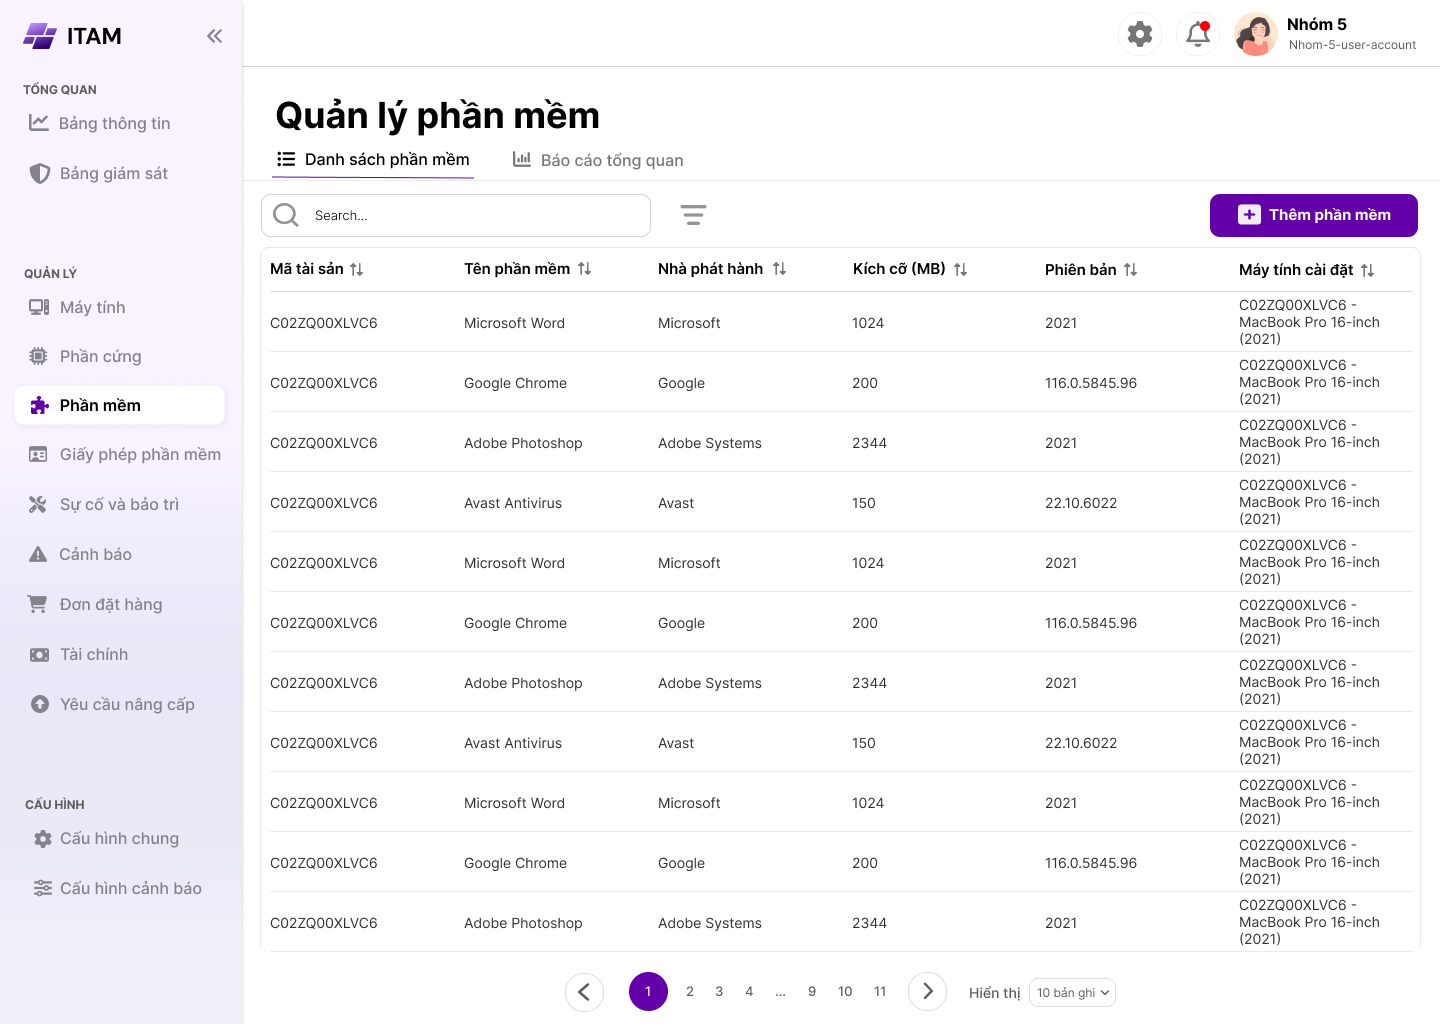
\includegraphics[width=14cm]{Images/C5/UI/Feature-Giám sát tài sản-Phần mềm 1.png}
%     \vspace{15pt}
%     \caption{Giao diện Quản lý phần mềm 1}
% \end{figure}
% \begin{figure}[H]
%     \centering
%     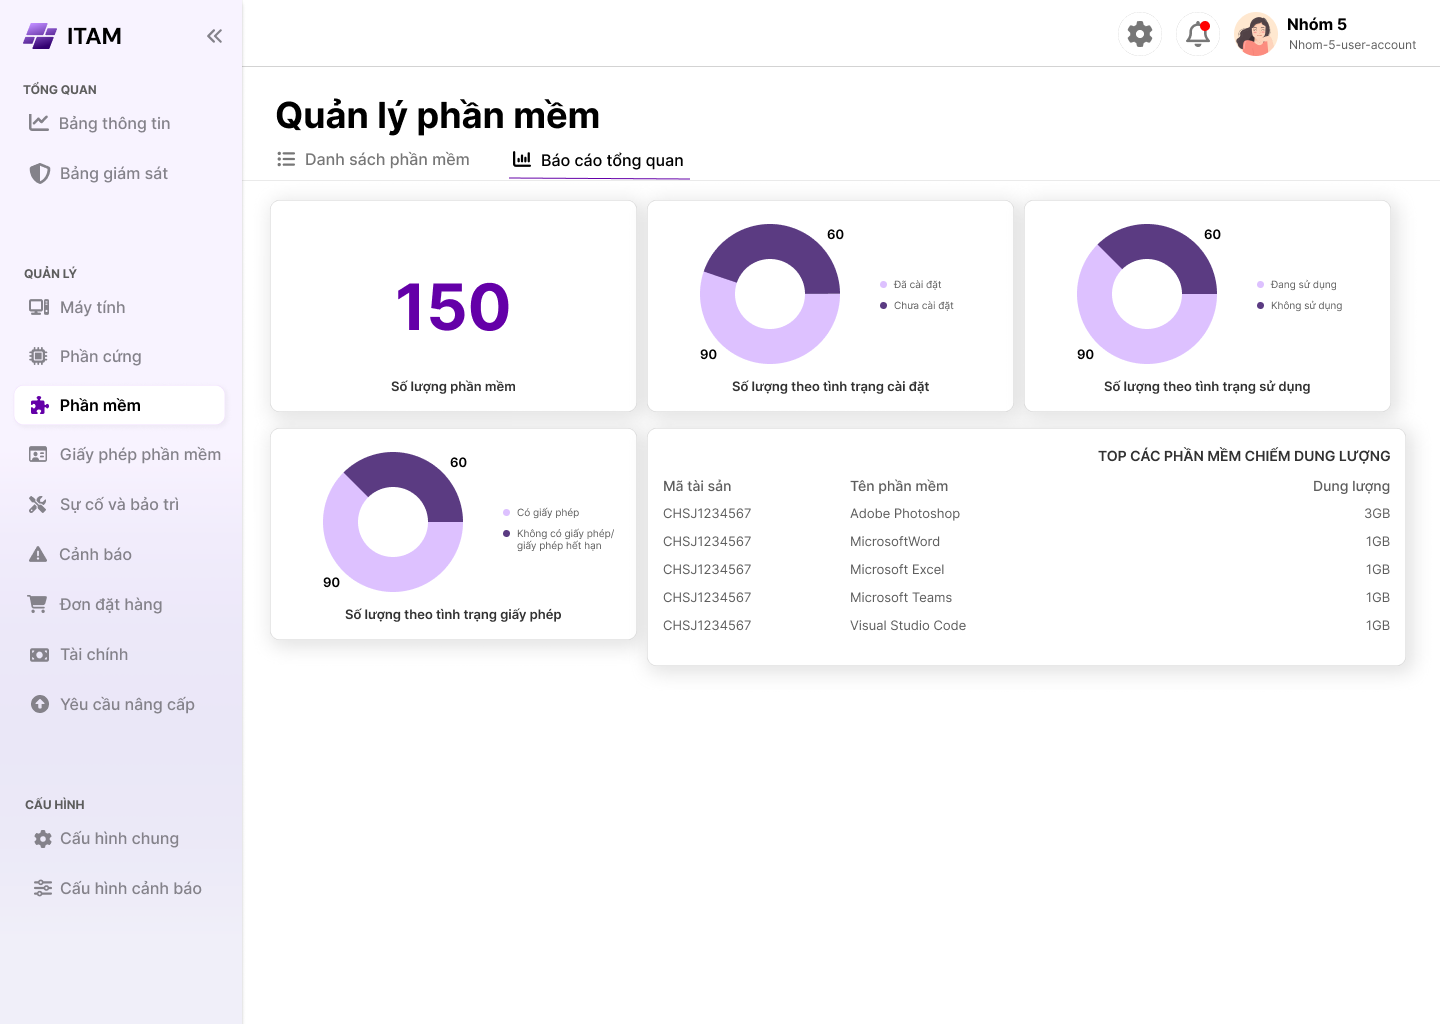
\includegraphics[width=14cm]{Images/C5/UI/Feature-Giám sát tài sản-Phần mềm 2.png}
%     \vspace{15pt}
%     \caption{Giao diện Quản lý phần mềm 2}
% \end{figure}
% \begin{figure}[H]
%     \centering
%     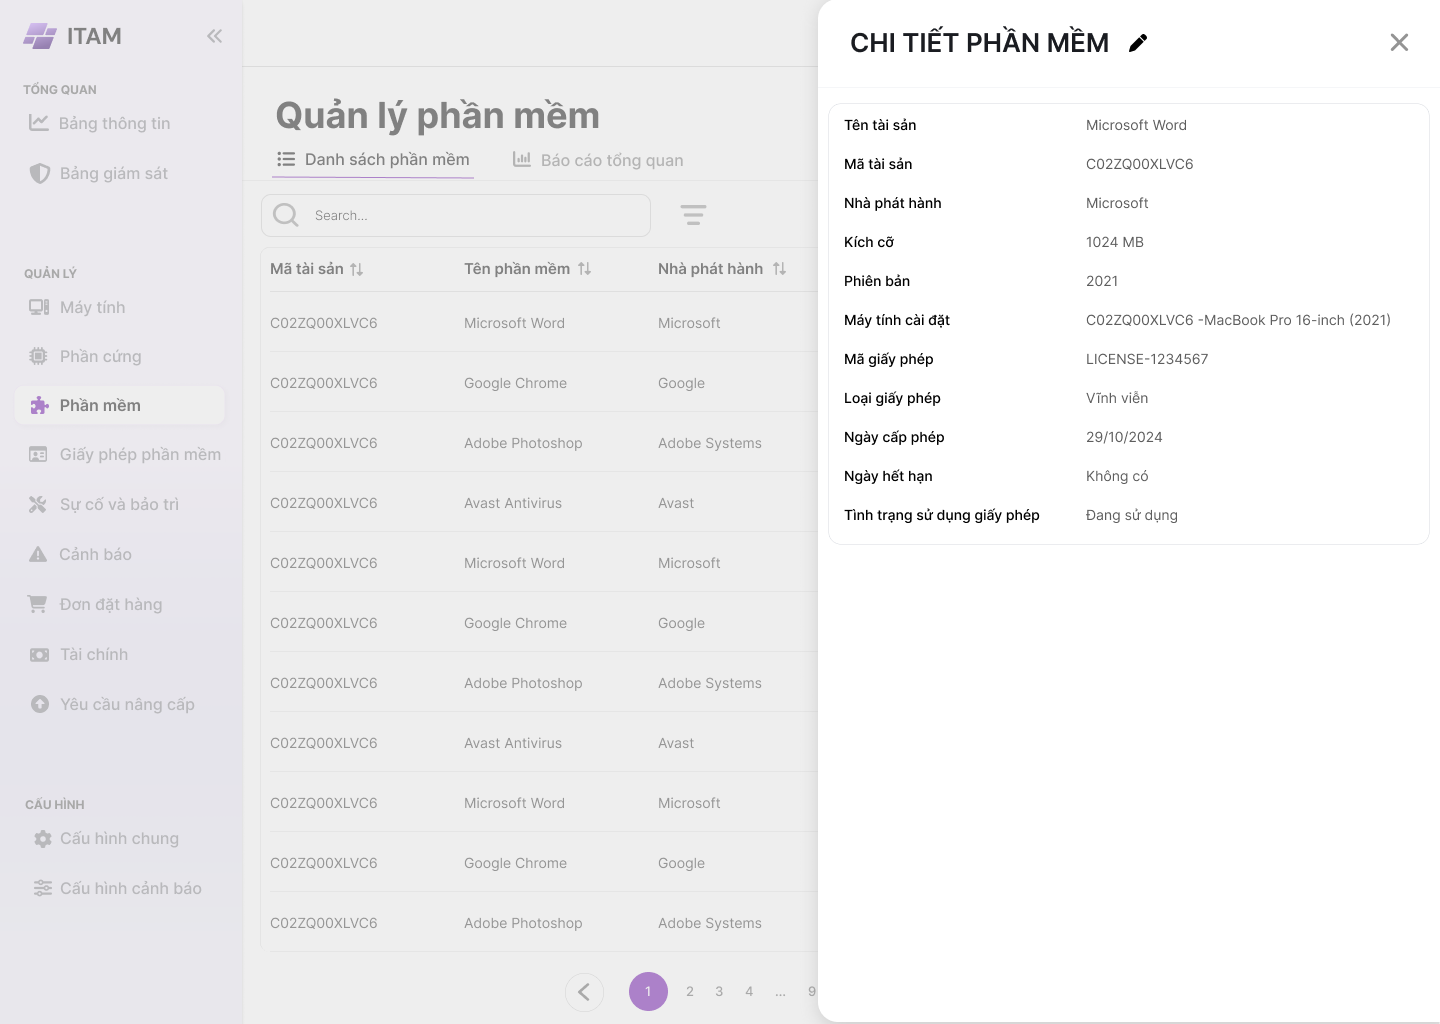
\includegraphics[width=14cm]{Images/C5/UI/Feature-Giám sát tài sản-Phần mềm 3.png}
%     \vspace{15pt}
%     \caption{Giao diện Quản lý phần mềm 3}
% \end{figure}
% \begin{figure}[H]
%     \centering
%     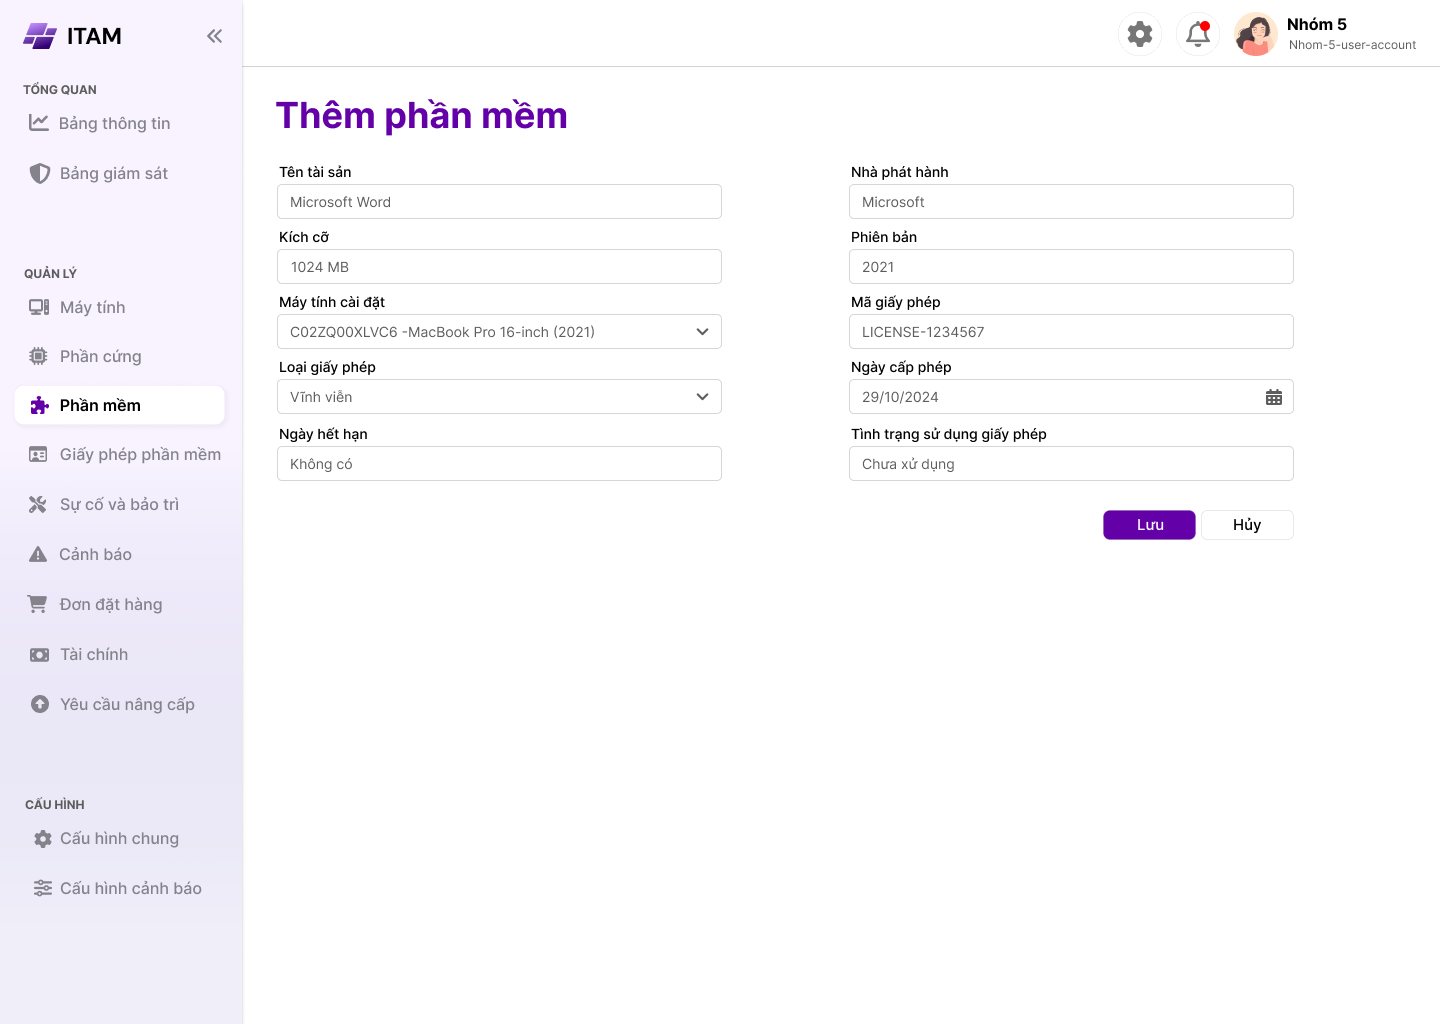
\includegraphics[width=14cm]{Images/C5/UI/Feature-Giám sát tài sản-Phần mềm 4.png}
%     \vspace{15pt}
%     \caption{Giao diện Quản lý phần mềm 4}
% \end{figure}

\item{Quản lý sự cố và bảo trì}\\
Quản lý sự cố và bảo trì cung cấp các tính năng xem danh sách, chi tiết sự cố và yêu cầu bảo trì của tài sản, giúp người dùng có thể quản lý một cách tập trung sự cố và bảo trì trong hệ thống (xem thêm chi tiết ở phụ lục).
% \begin{figure}[H]
%     \centering
%     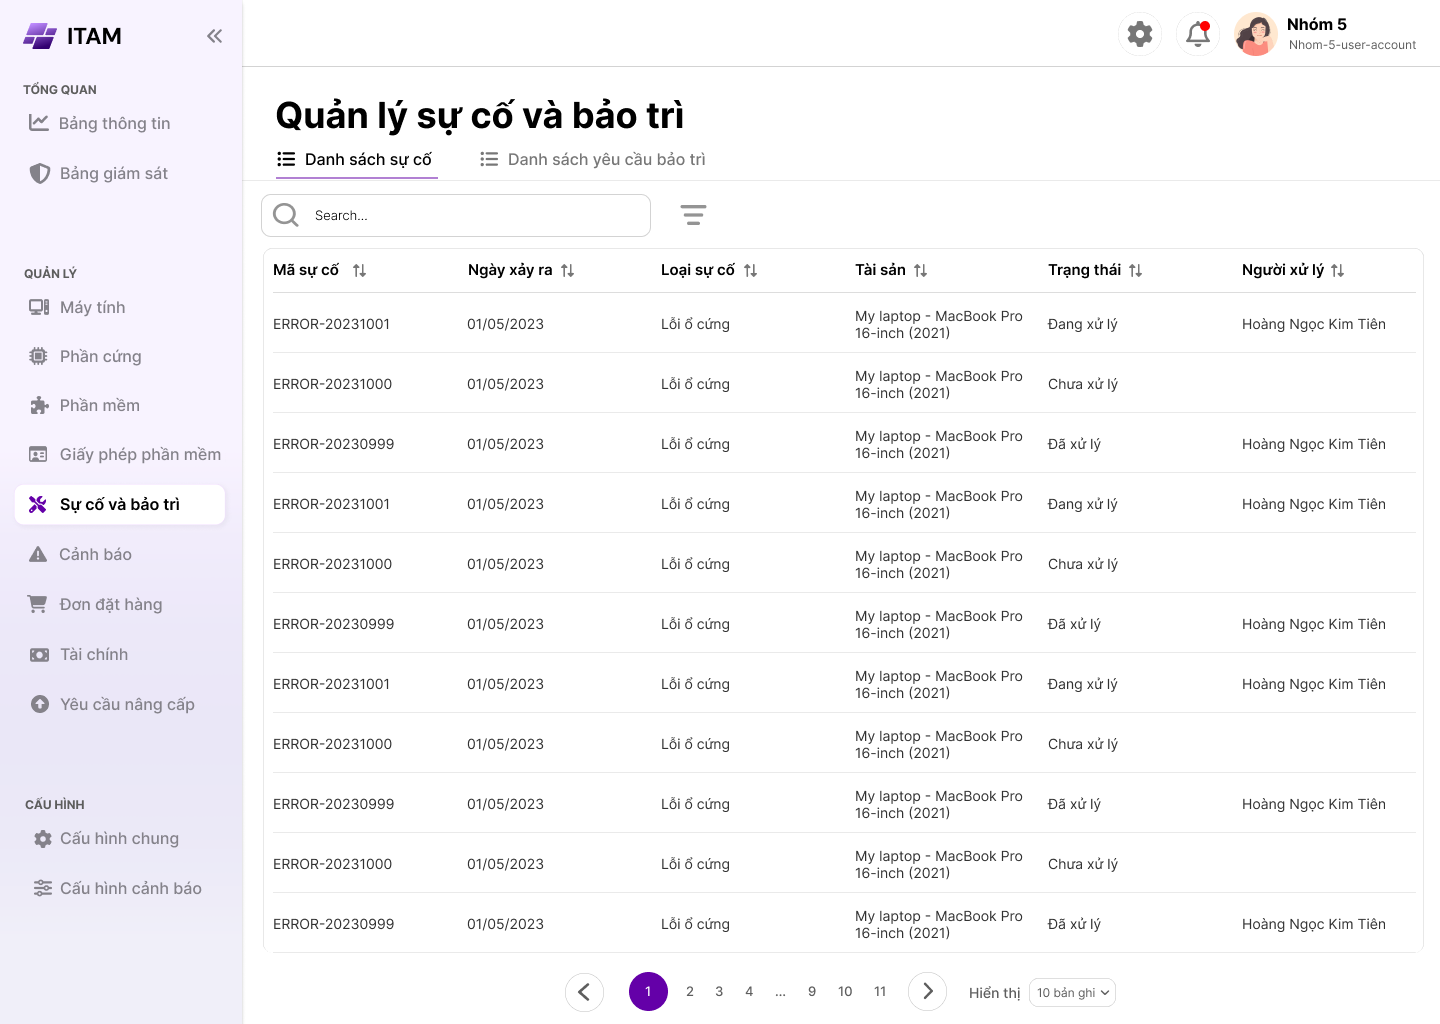
\includegraphics[width=14cm]{Images/C5/UI/Feature-Quản lý sự cố và bảo trì 1.png}
%     \vspace{15pt}
%     \caption{Giao diện Quản lý sự cố và bảo trì 1}
% \end{figure}
% \begin{figure}[H]
%     \centering
%     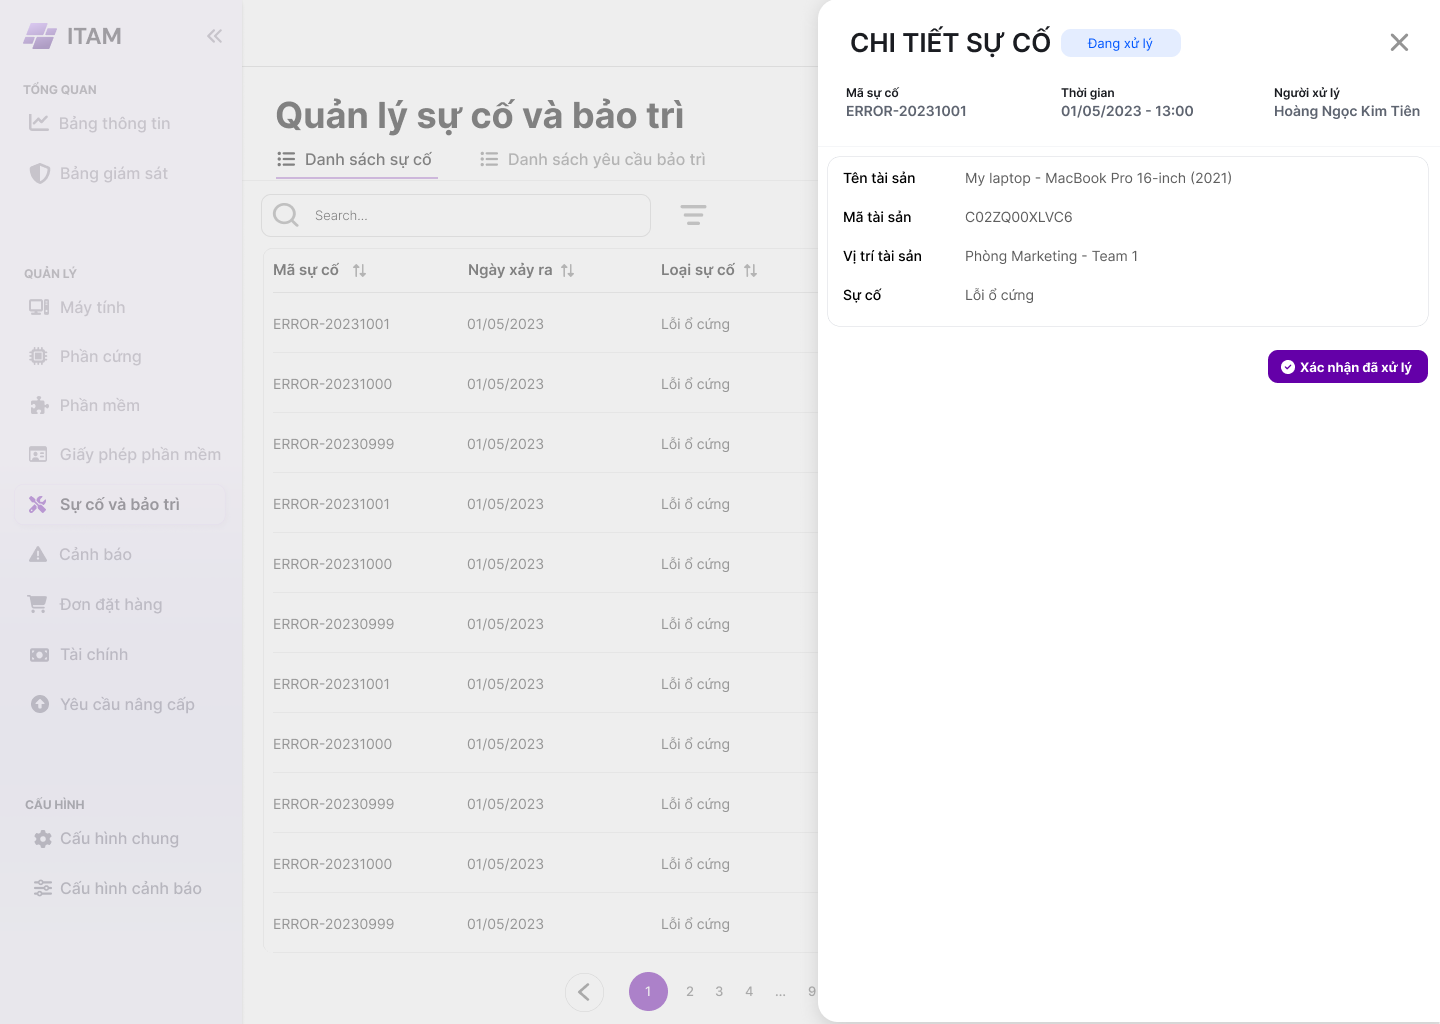
\includegraphics[width=14cm]{Images/C5/UI/Feature-Quản lý sự cố và bảo trì 2.1.png}
%     \vspace{15pt}
%     \caption{Giao diện Quản lý sự cố và bảo trì 2}
% \end{figure}
% \begin{figure}[H]
%     \centering
%     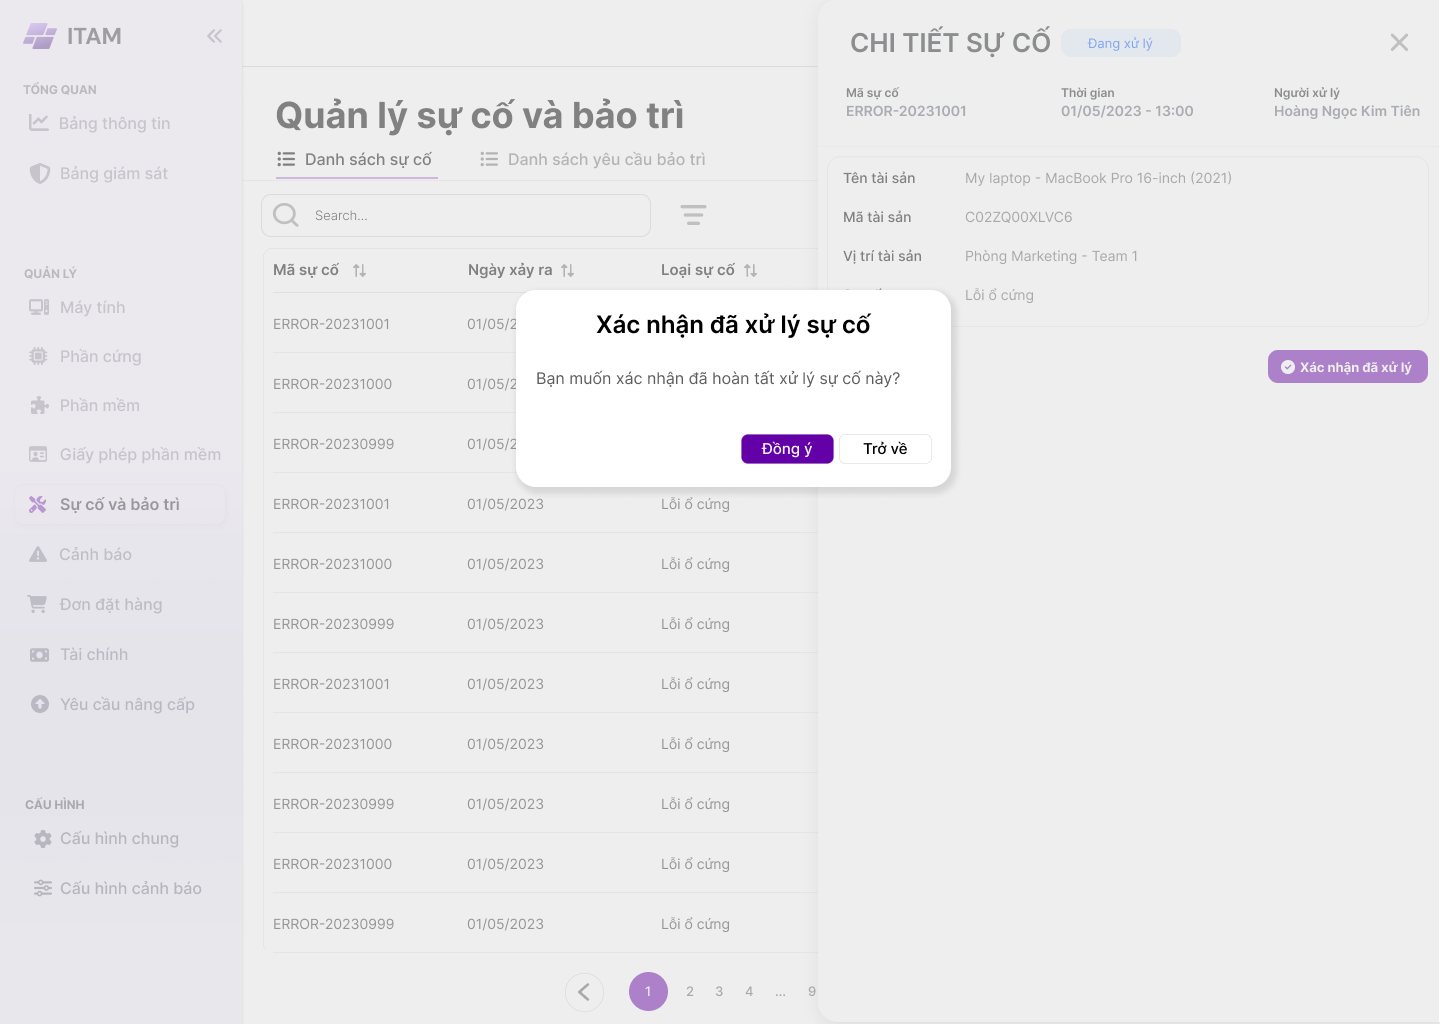
\includegraphics[width=14cm]{Images/C5/UI/Feature-Quản lý sự cố và bảo trì 2.2.png}
%     \vspace{15pt}
%     \caption{Giao diện Quản lý sự cố và bảo trì 3}
% \end{figure}
% \begin{figure}[H]
%     \centering
%     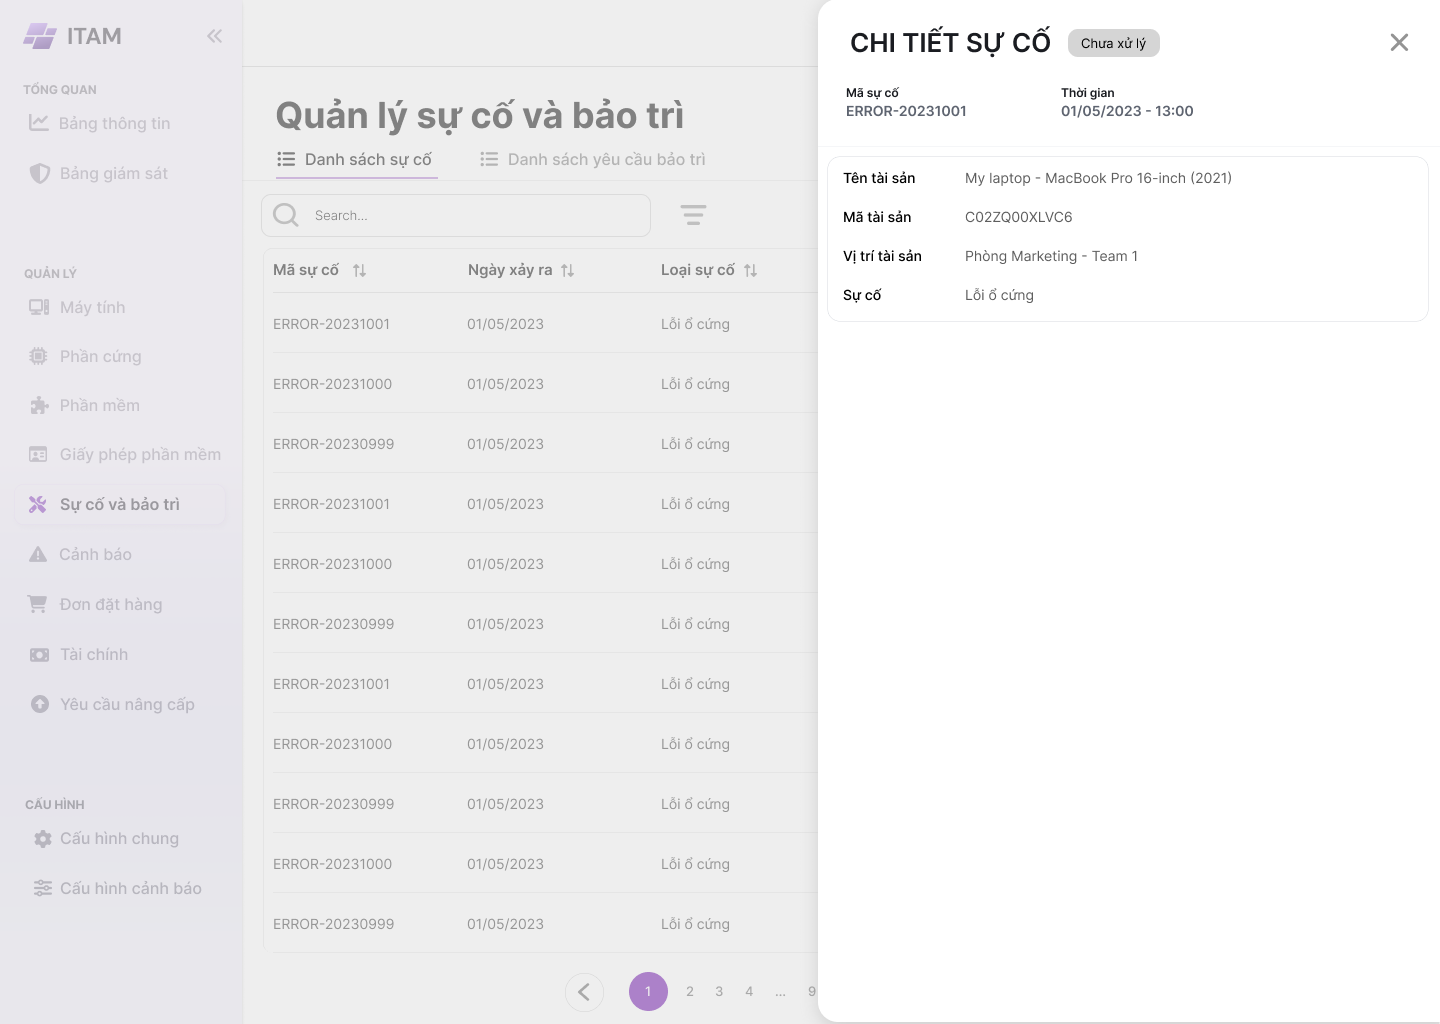
\includegraphics[width=14cm]{Images/C5/UI/Feature-Quản lý sự cố và bảo trì 2.3.png}
%     \vspace{15pt}
%     \caption{Giao diện Quản lý sự cố và bảo trì 4}
% \end{figure}
% \begin{figure}[H]
%     \centering
%     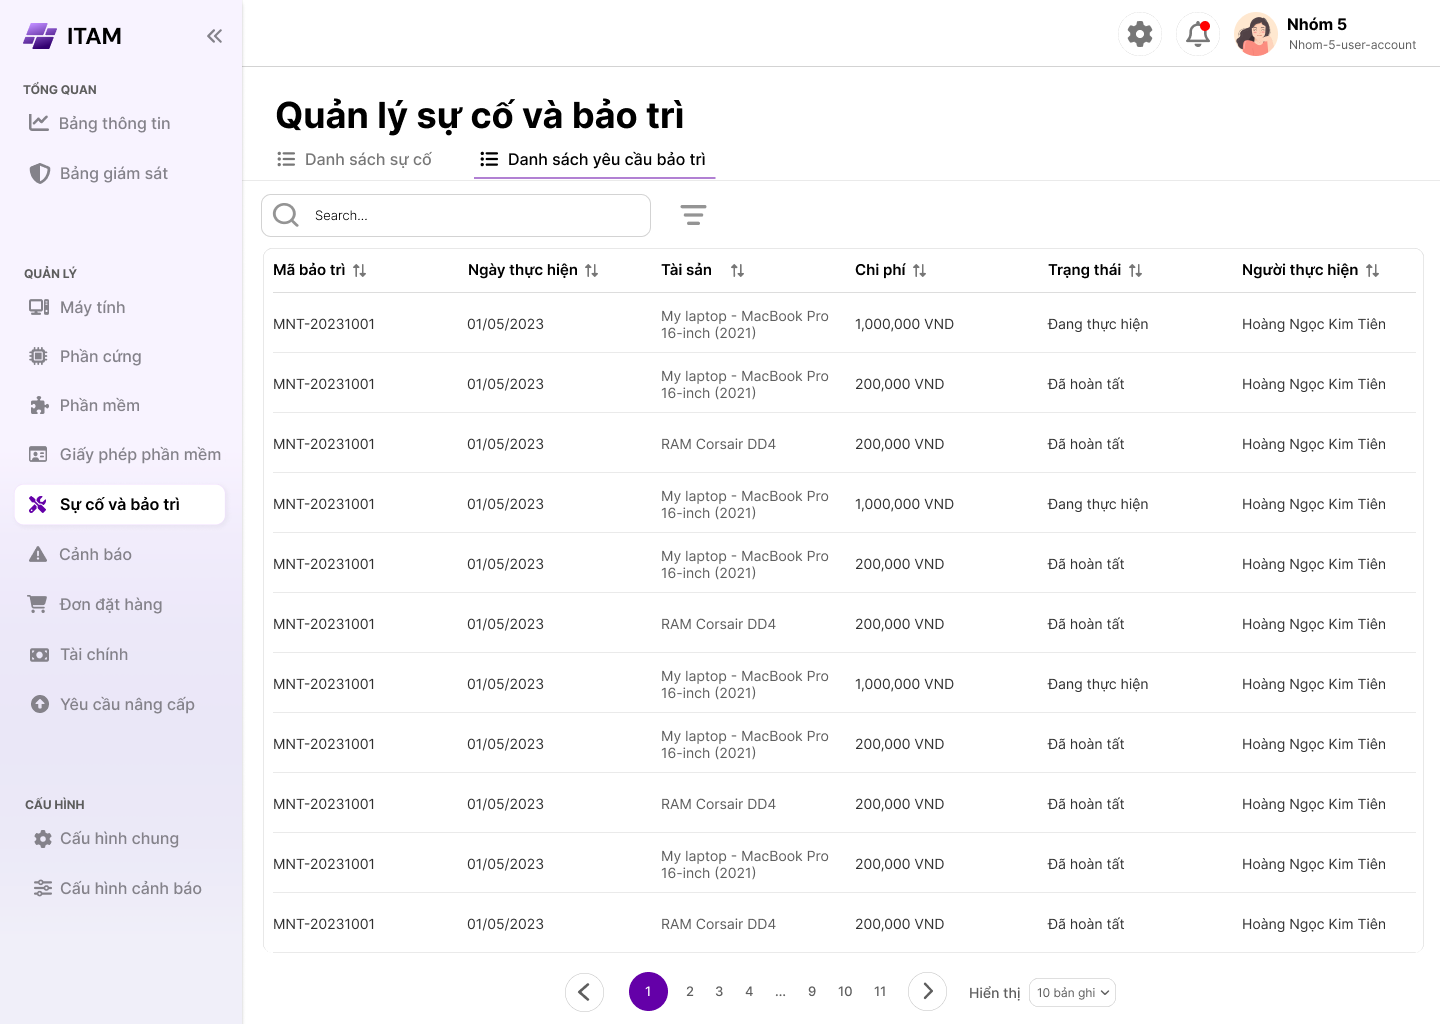
\includegraphics[width=14cm]{Images/C5/UI/Feature-Quản lý sự cố và bảo trì 3.1.png}
%     \vspace{15pt}
%     \caption{Giao diện Quản lý sự cố và bảo trì 3}
% \end{figure}
% \begin{figure}[H]
%     \centering
%     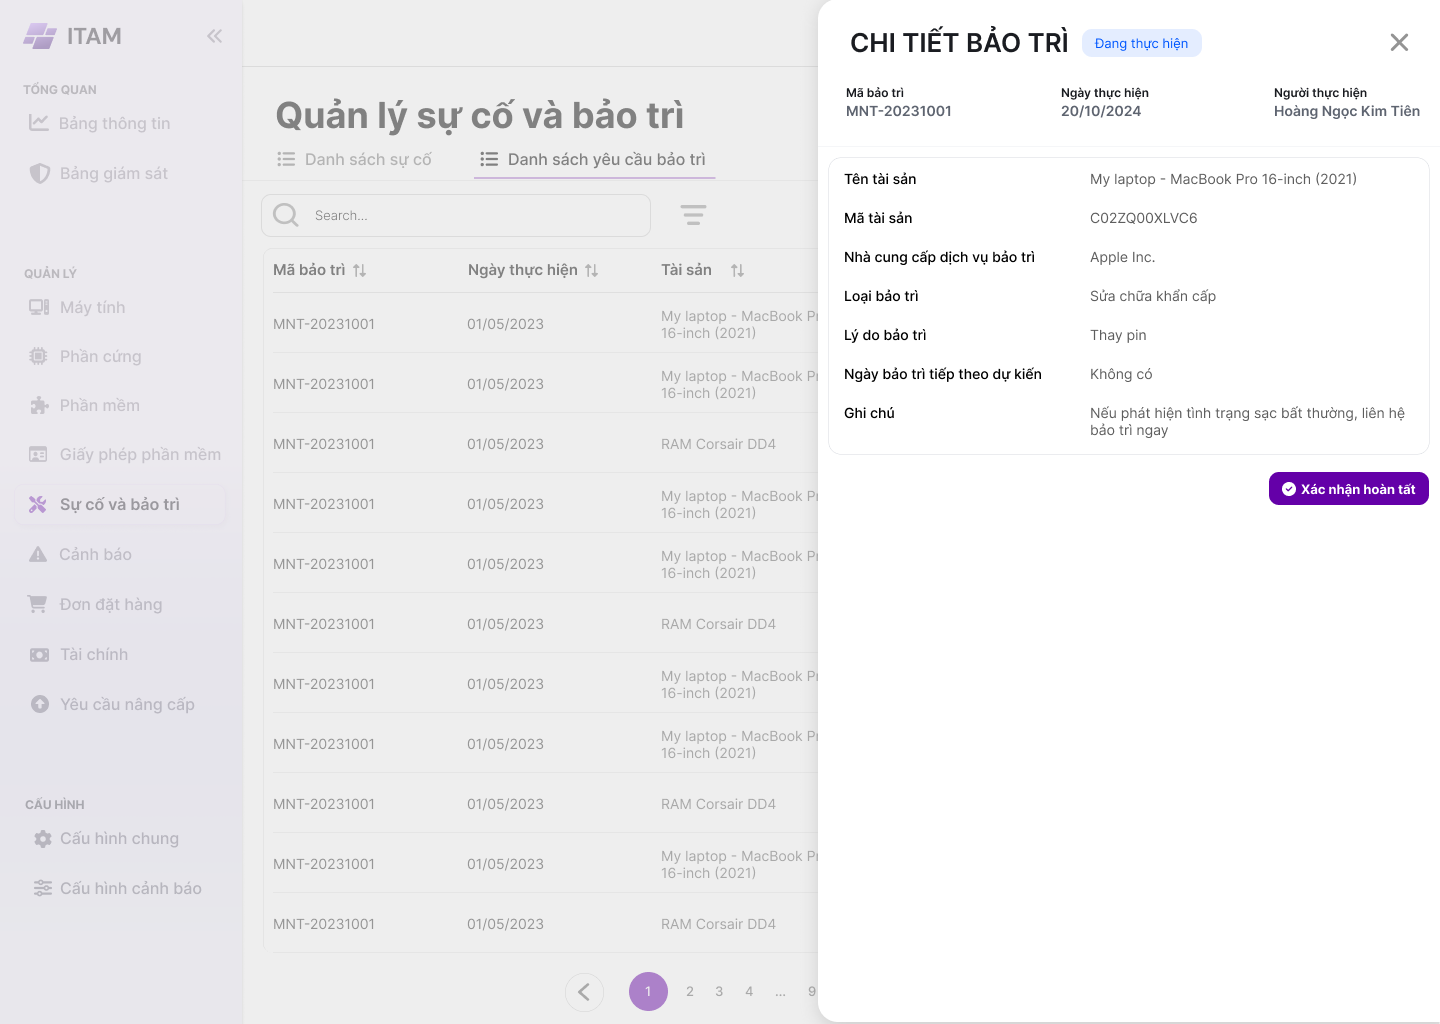
\includegraphics[width=14cm]{Images/C5/UI/Feature-Quản lý sự cố và bảo trì 3.2.png}
%     \vspace{15pt}
%     \caption{Giao diện Quản lý sự cố và bảo trì 4}
% \end{figure}
% \begin{figure}[H]
%     \centering
%     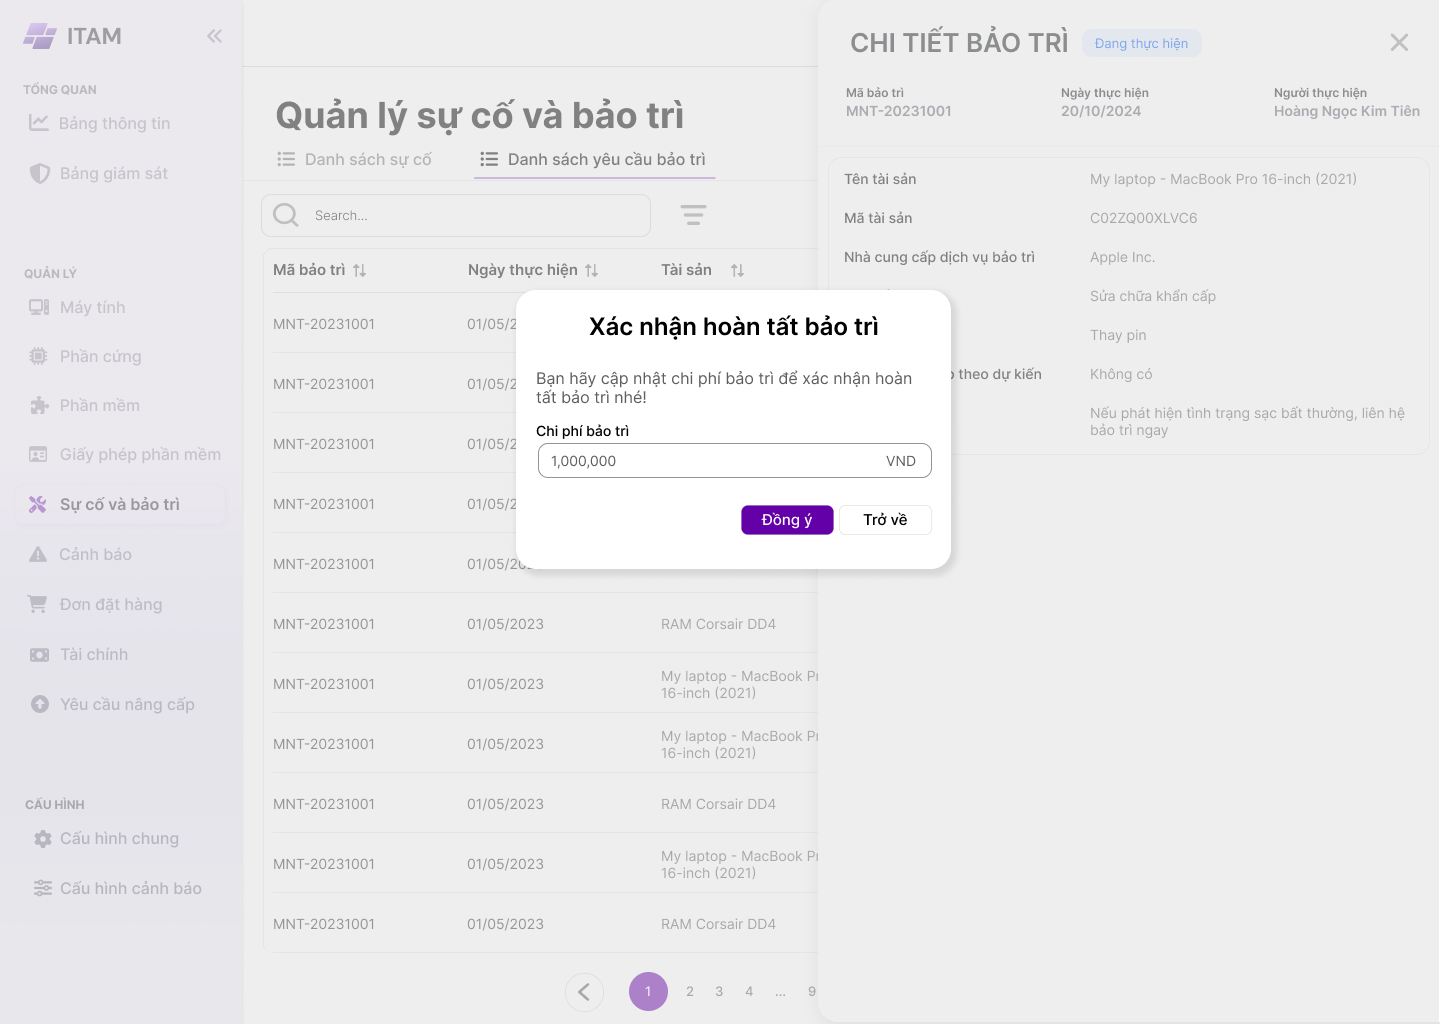
\includegraphics[width=14cm]{Images/C5/UI/Feature-Quản lý sự cố và bảo trì 3.3.png}
%     \vspace{15pt}
%     \caption{Giao diện Quản lý sự cố và bảo trì 7}
% \end{figure}

\item{Quản lý cảnh báo}\\
Ở Quản lý cảnh báo, người cùng có thể xem tất cả các cảnh báo của các máy tính có trong hệ thống và xem chi tiết các cảnh báo đó. Cảnh báo cũng được phân loại màu sắc dựa trên mức độ nghiêm trọng để người dùng có thể kịp thời đưa ra quyết định xử lý các cảnh báo quan trọng (xem thêm chi tiết ở phụ lục).
% \begin{figure}[H]
%     \centering
%     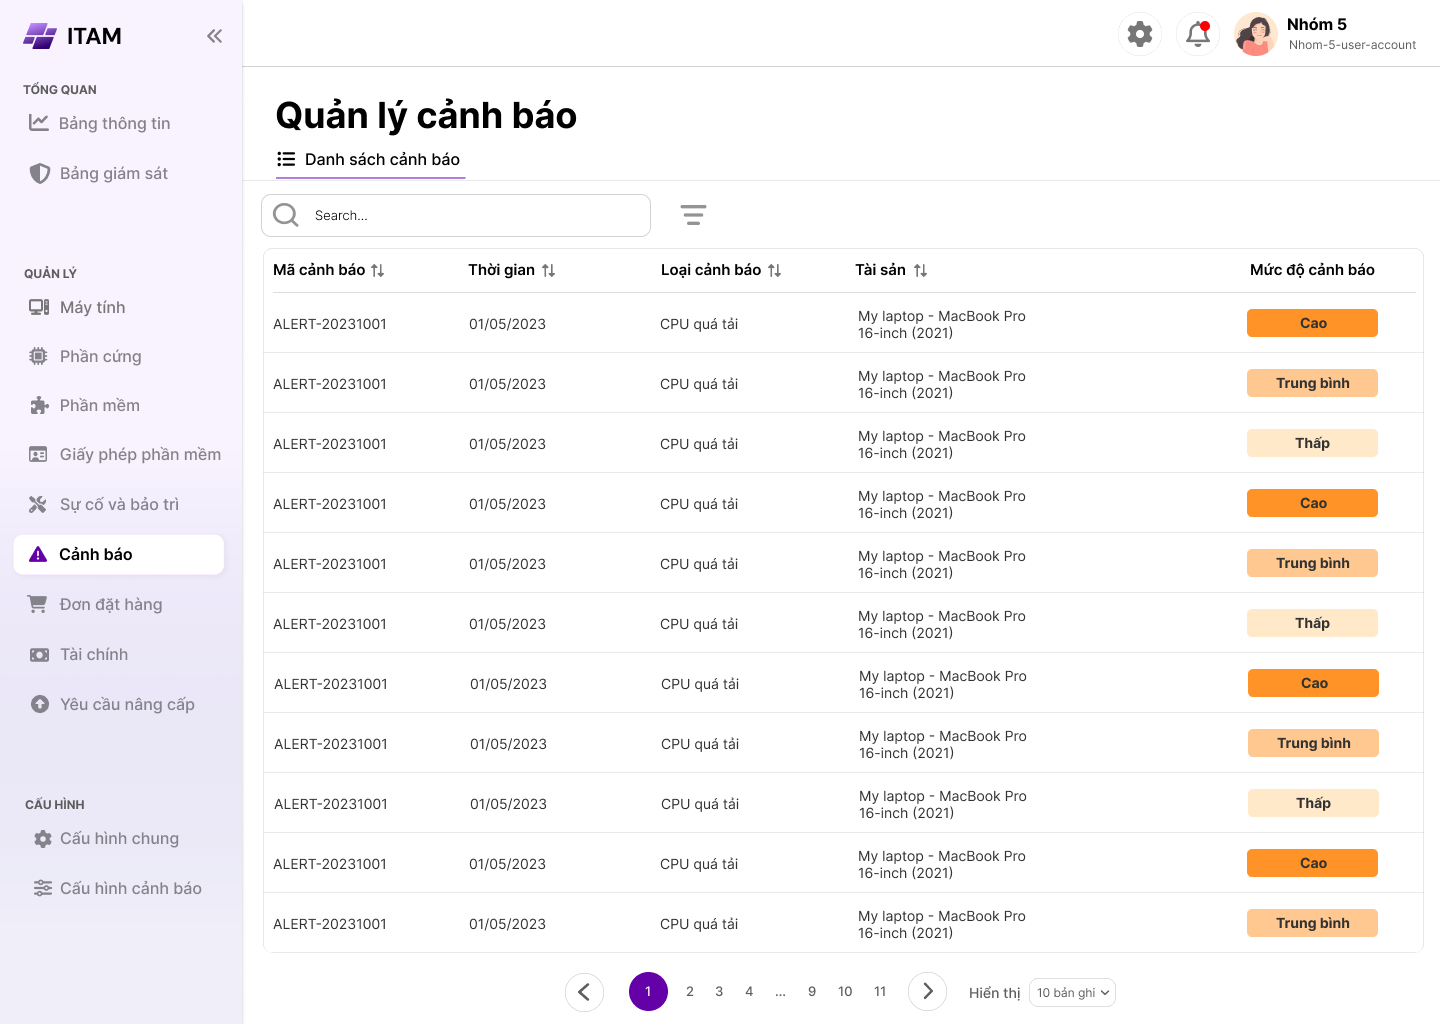
\includegraphics[width=14cm]{Images/C5/UI/Feature-Quản lý cảnh báo 1.png}
%     \vspace{15pt}
%     \caption{Giao diện Quản lý cảnh báo 1}
% \end{figure}
% \begin{figure}[H]
%     \centering
%     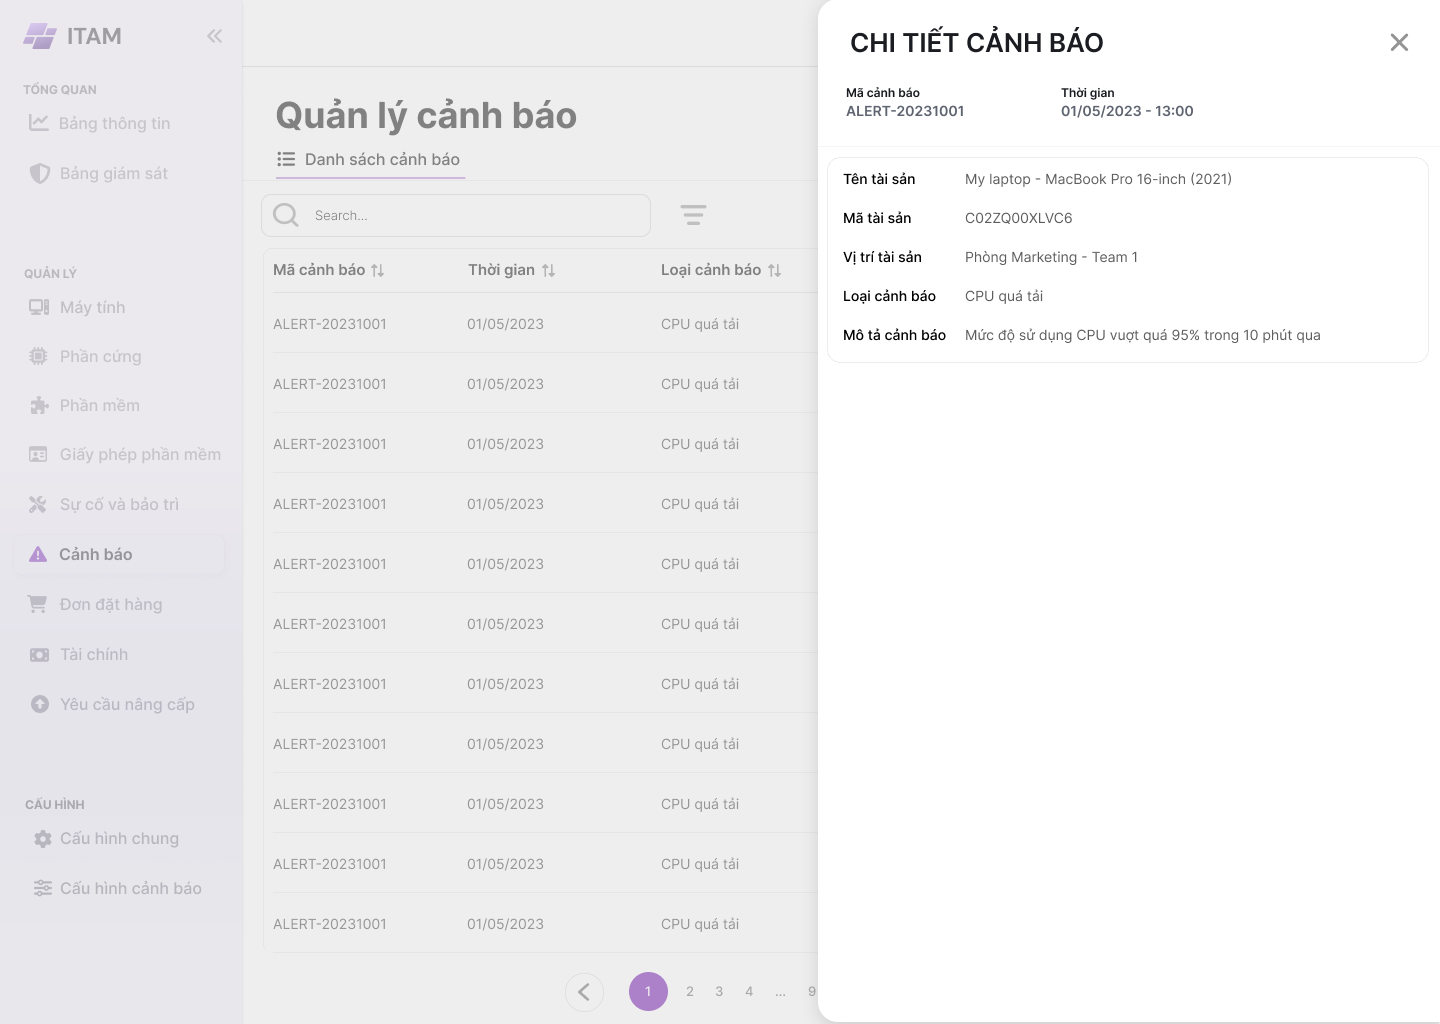
\includegraphics[width=14cm]{Images/C5/UI/Feature-Quản lý cảnh báo 2.1.png}
%     \vspace{15pt}
%     \caption{Giao diện Quản lý cảnh báo 2}
% \end{figure}

\item{Quản lý yêu cầu nâng cấp}\\
Người dùng có thể xem danh sách các yêu cầu nâng cấp và chi tiết các yêu cầu nâng cấp đó, đồng thời quản lý cũng có thể phê duyệt các yêu cầu nâng cấp (xem thêm chi tiết ở phụ lục).
% \begin{figure}[H]
%     \centering
%     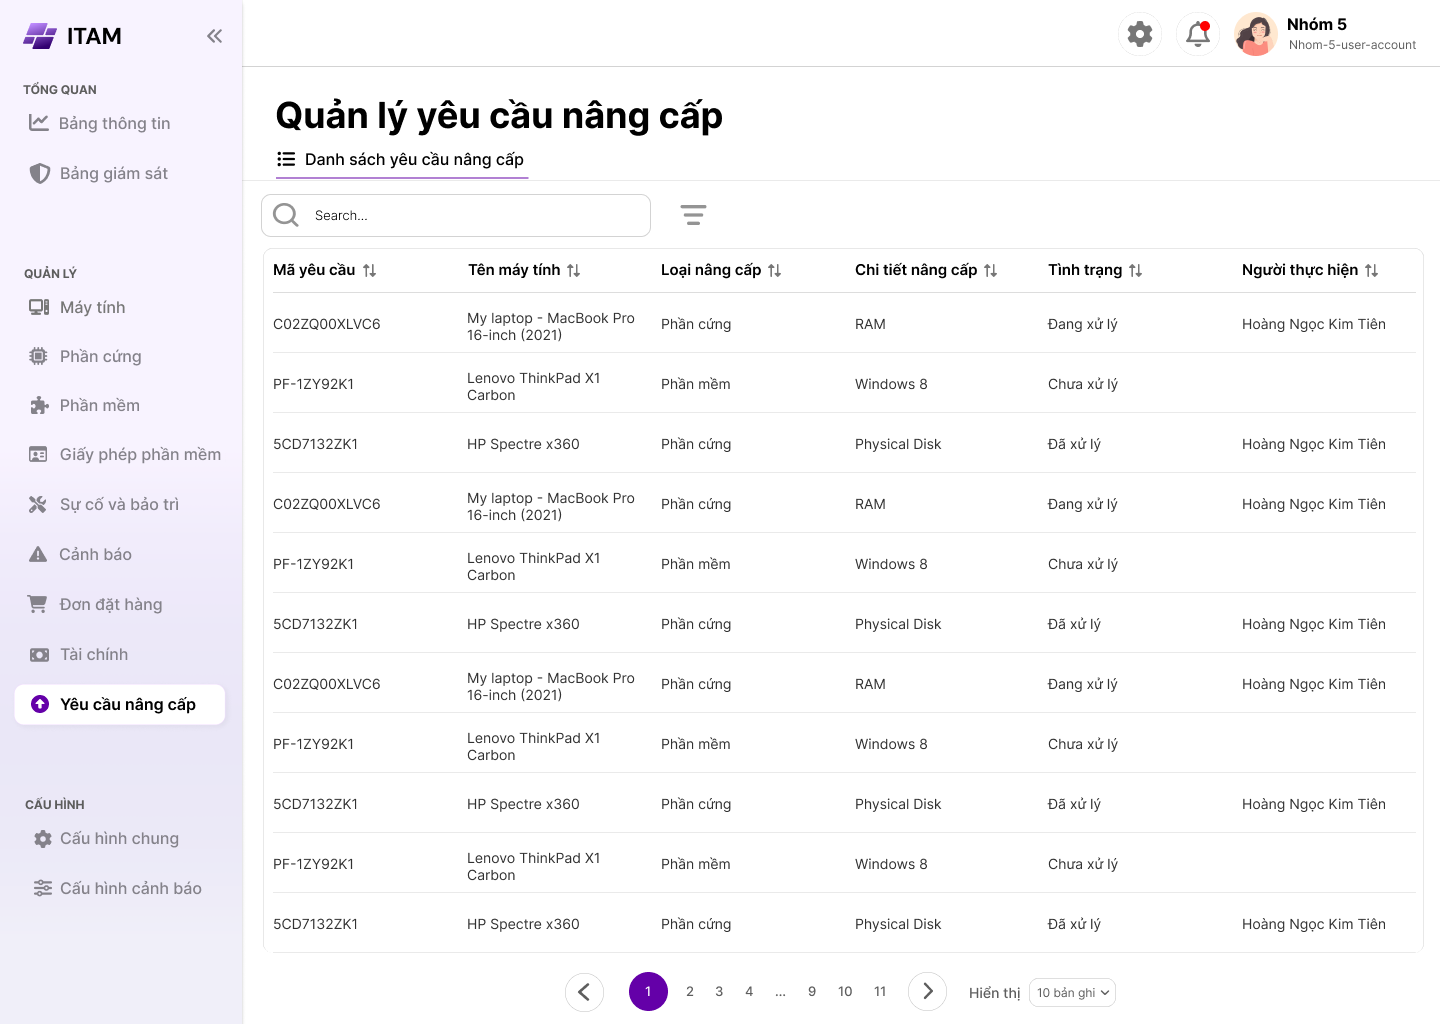
\includegraphics[width=14cm]{Images/C5/UI/Feature-Quản lý yêu cầu nâng cấp 1.png}
%     \vspace{15pt}
%     \caption{Giao diện Quản lý yêu cầu nâng cấp 1}
% \end{figure}
% \begin{figure}[H]
%     \centering
%     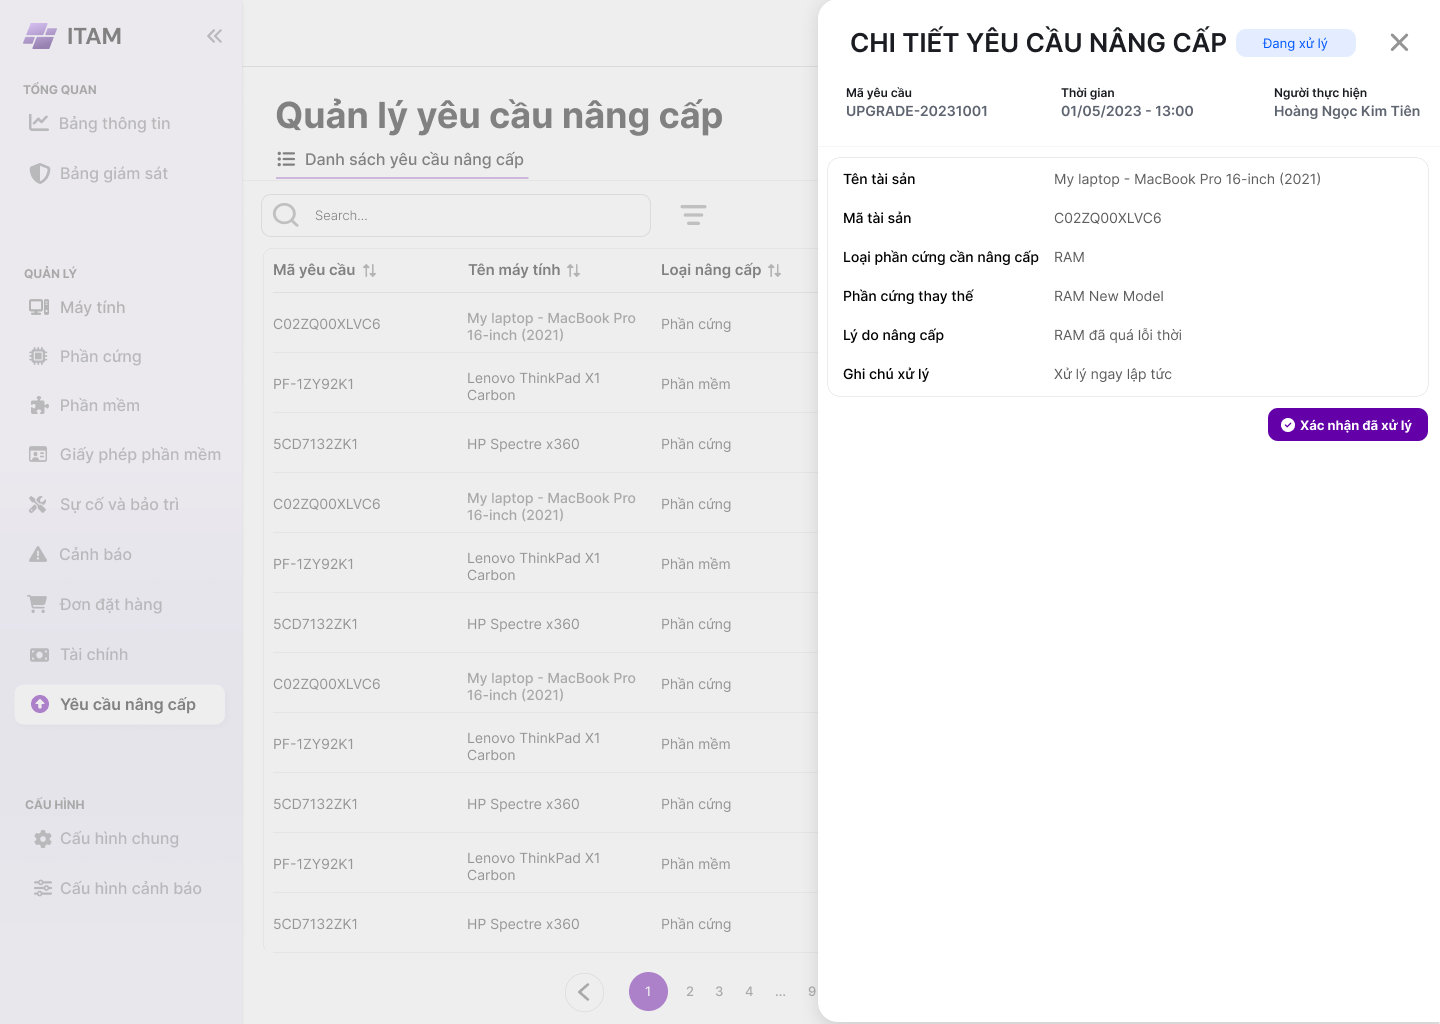
\includegraphics[width=14cm]{Images/C5/UI/Feature-Quản lý yêu cầu nâng cấp 2.1.png}
%     \vspace{15pt}
%     \caption{Giao diện Quản lý yêu cầu nâng cấp 2}
% \end{figure}
% \begin{figure}[H]
%     \centering
%     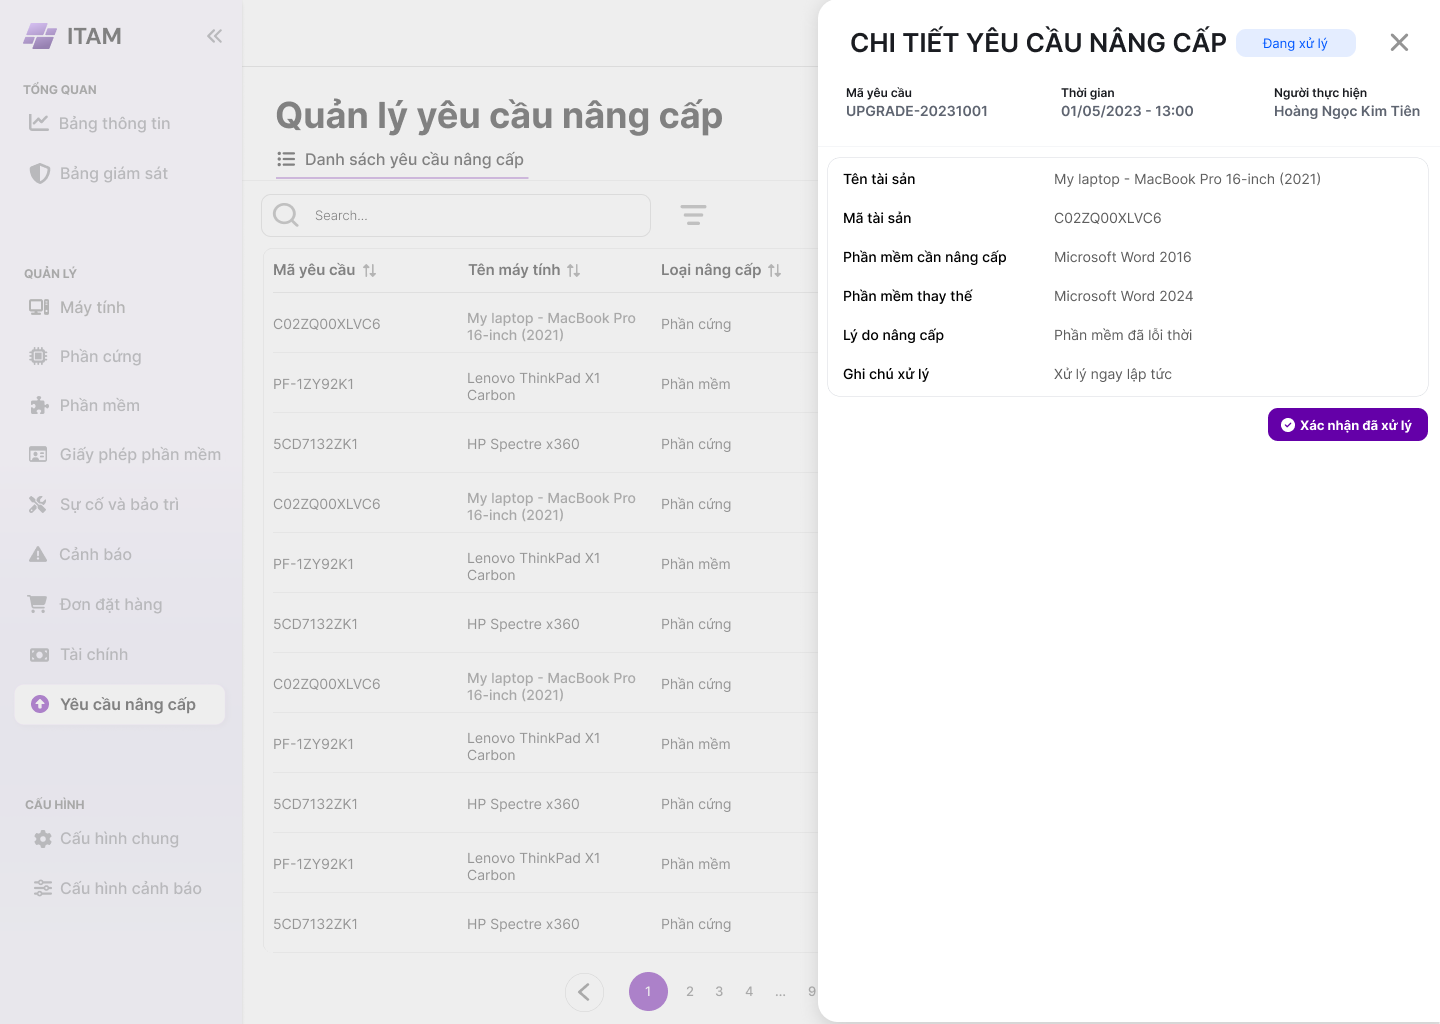
\includegraphics[width=14cm]{Images/C5/UI/Feature-Quản lý yêu cầu nâng cấp 2.2.png}
%     \vspace{15pt}
%     \caption{Giao diện Quản lý yêu cầu nâng cấp 3}
% \end{figure}
% \begin{figure}[H]
%     \centering
%     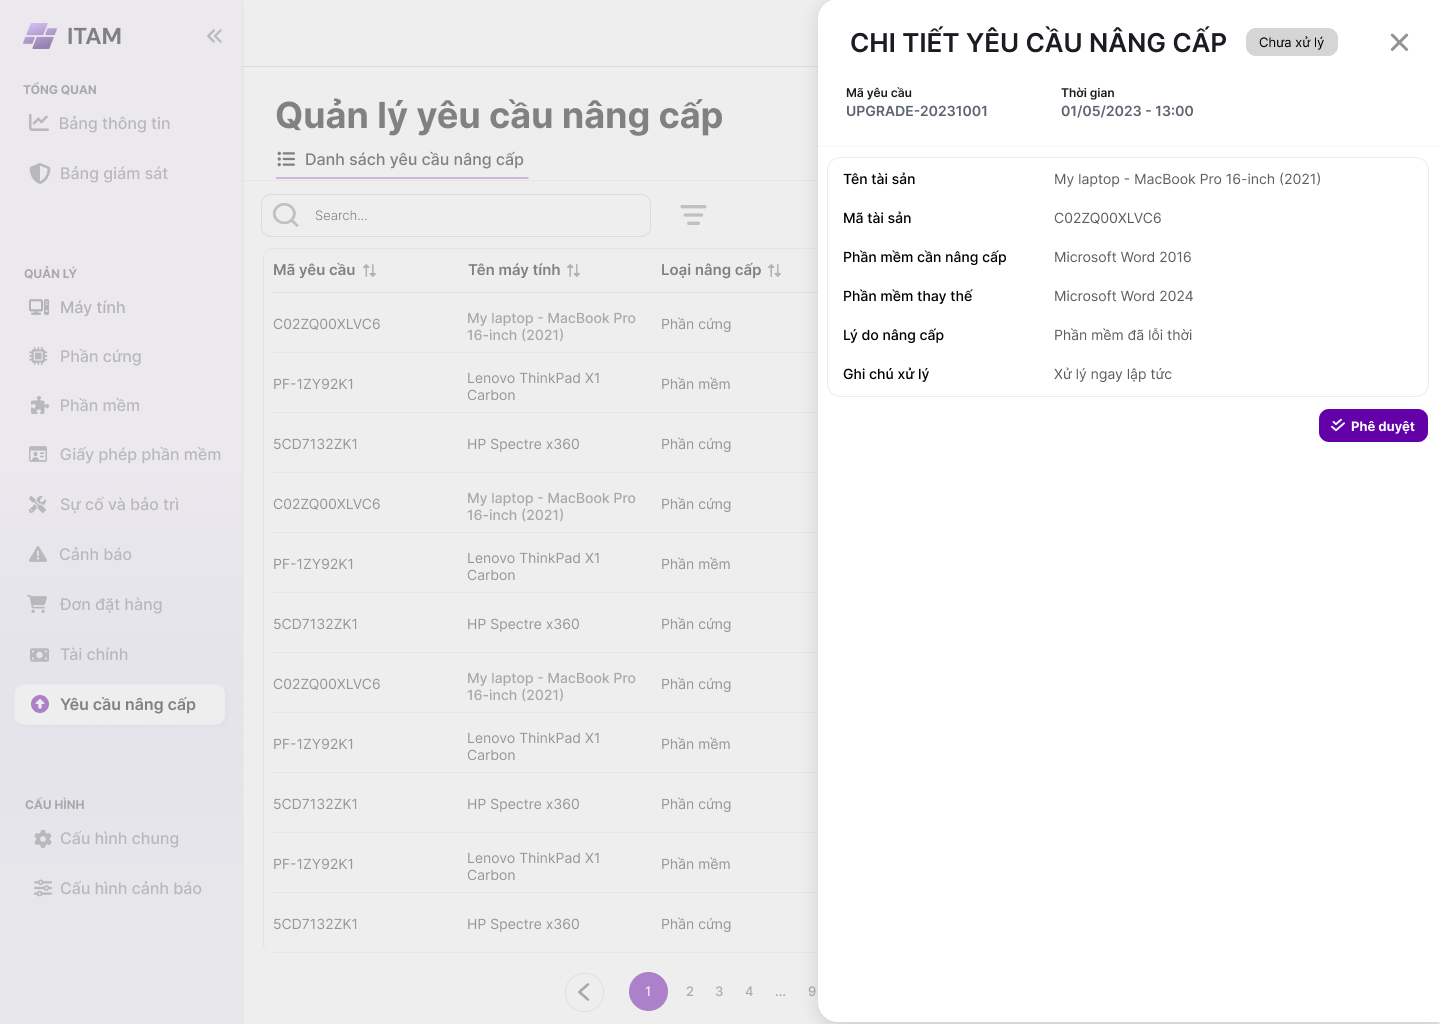
\includegraphics[width=14cm]{Images/C5/UI/Feature-Quản lý yêu cầu nâng cấp 2.3.png}
%     \vspace{15pt}
%     \caption{Giao diện Quản lý yêu cầu nâng cấp 2}
% \end{figure}
% \begin{figure}[H]
%     \centering
%     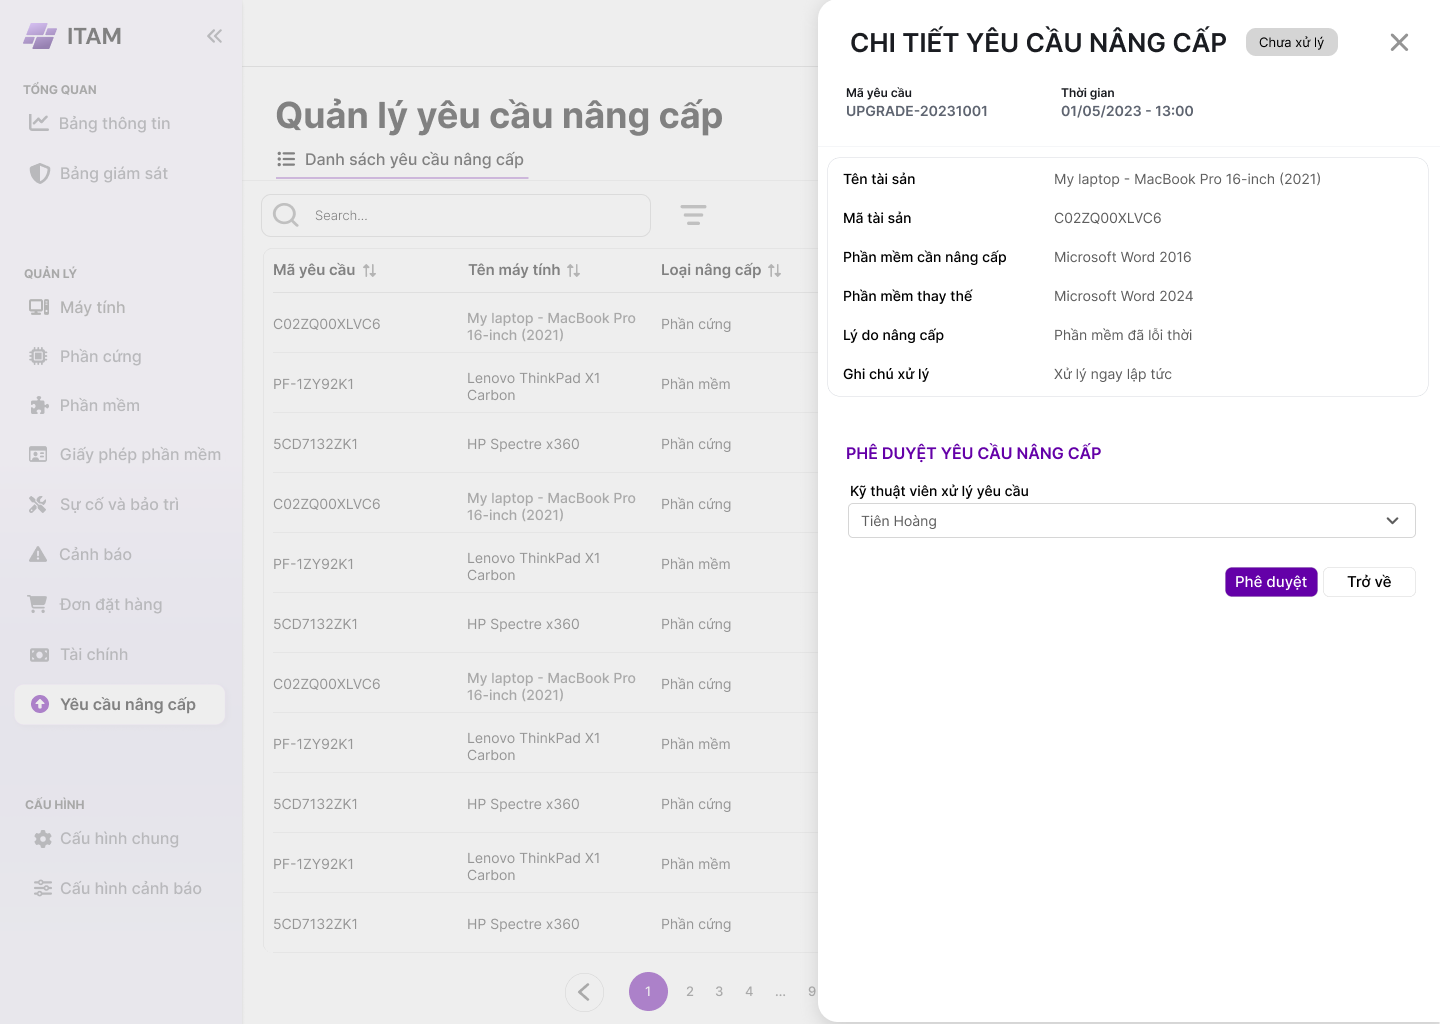
\includegraphics[width=14cm]{Images/C5/UI/Feature-Quản lý yêu cầu nâng cấp 2.4.png}
%     \vspace{15pt}
%     \caption{Giao diện Quản lý yêu cầu nâng cấp 2}
% \end{figure}

\item{Quản lý yêu cầu thanh lý}\\
Người dùng có thể xem danh sách các yêu cầu thanh lý và chi tiết các yêu cầu thanh lý đó, đồng thời quản lý cũng có thể phê duyệt các yêu cầu thanh lý (xem thêm chi tiết ở phụ lục).

\item{Quản lý đơn đặt hàng}\\
Người dùng với vai trò quản lý có thể xem danh sách đơn đặt hàng và chi tiết đơn đặt hàng, tạo đơn đặt hàng mới (xem thêm chi tiết ở phụ lục).
% \begin{figure}[H]
%     \centering
%     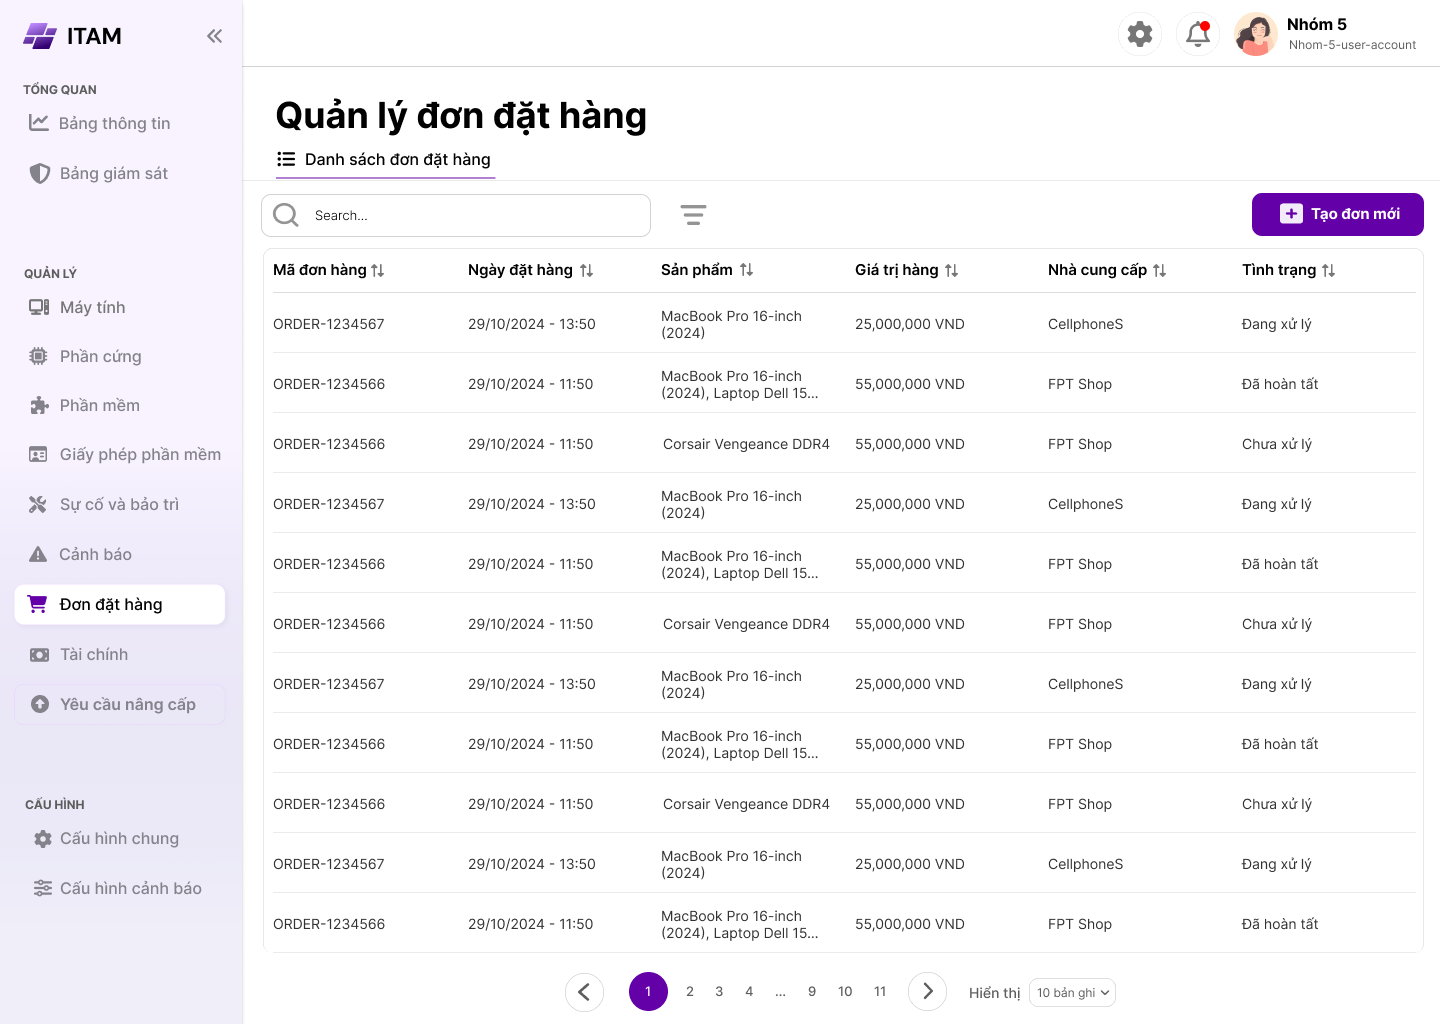
\includegraphics[width=14cm]{Images/C5/UI/Feature-Quản lý đơn đặt hàng 1.png}
%     \vspace{15pt}
%     \caption{Giao diện Quản lý đơn đặt hàng 1}
% \end{figure}
% \begin{figure}[H]
%     \centering
%     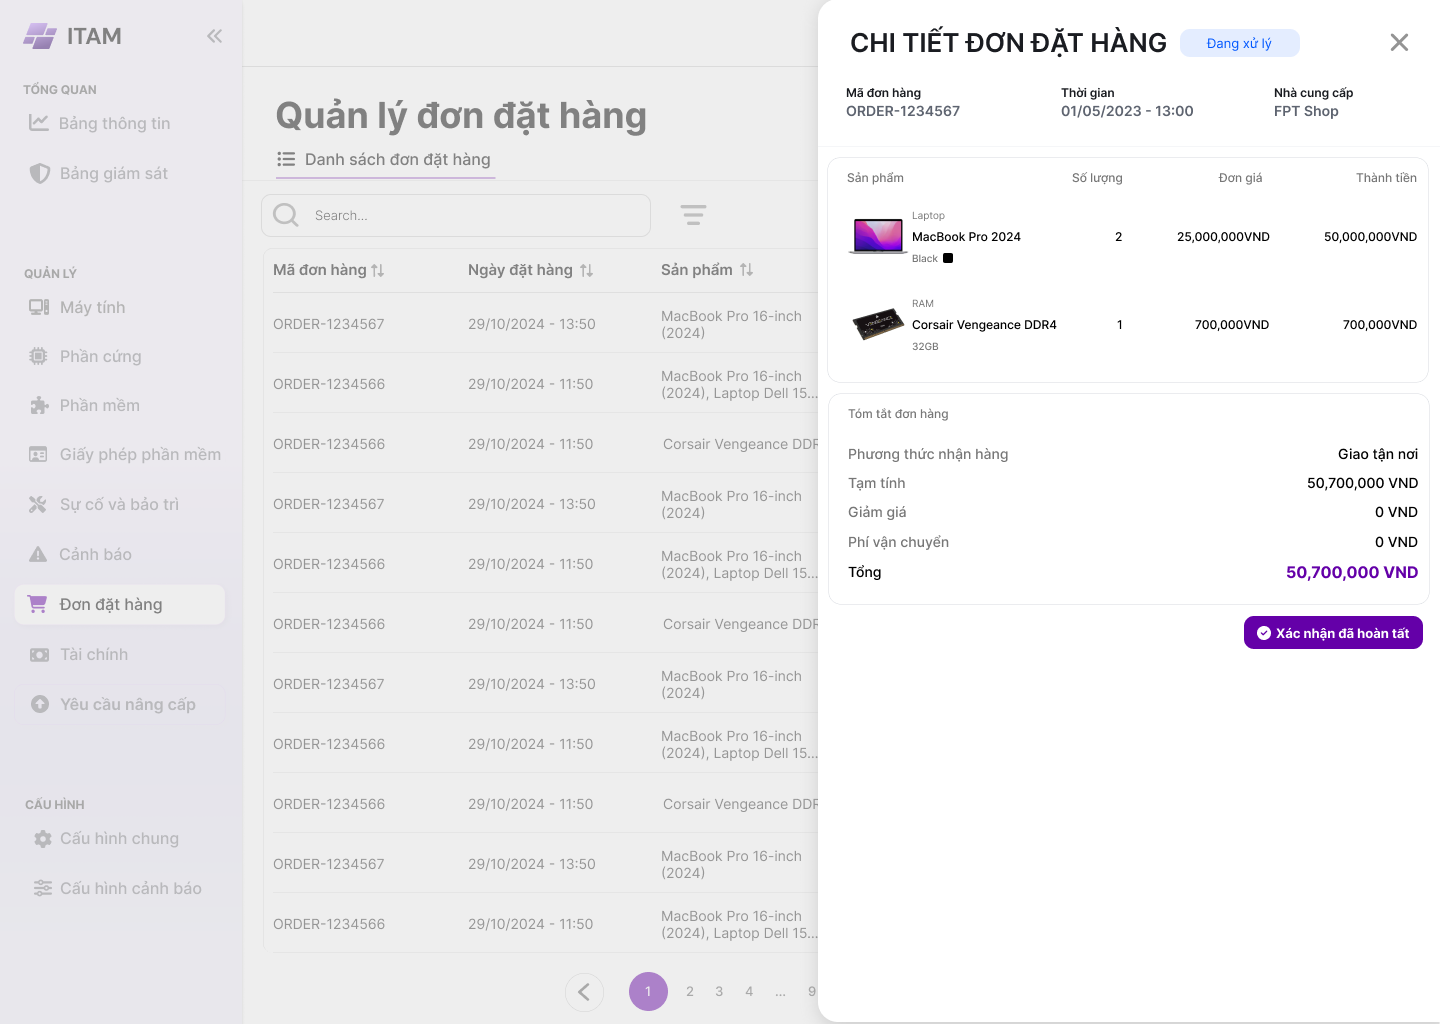
\includegraphics[width=14cm]{Images/C5/UI/Feature-Quản lý đơn đặt hàng 2.1.png}
%     \vspace{15pt}
%     \caption{Giao diện Quản lý đơn đặt hàng 2}
% \end{figure}
% \begin{figure}[H]
%     \centering
%     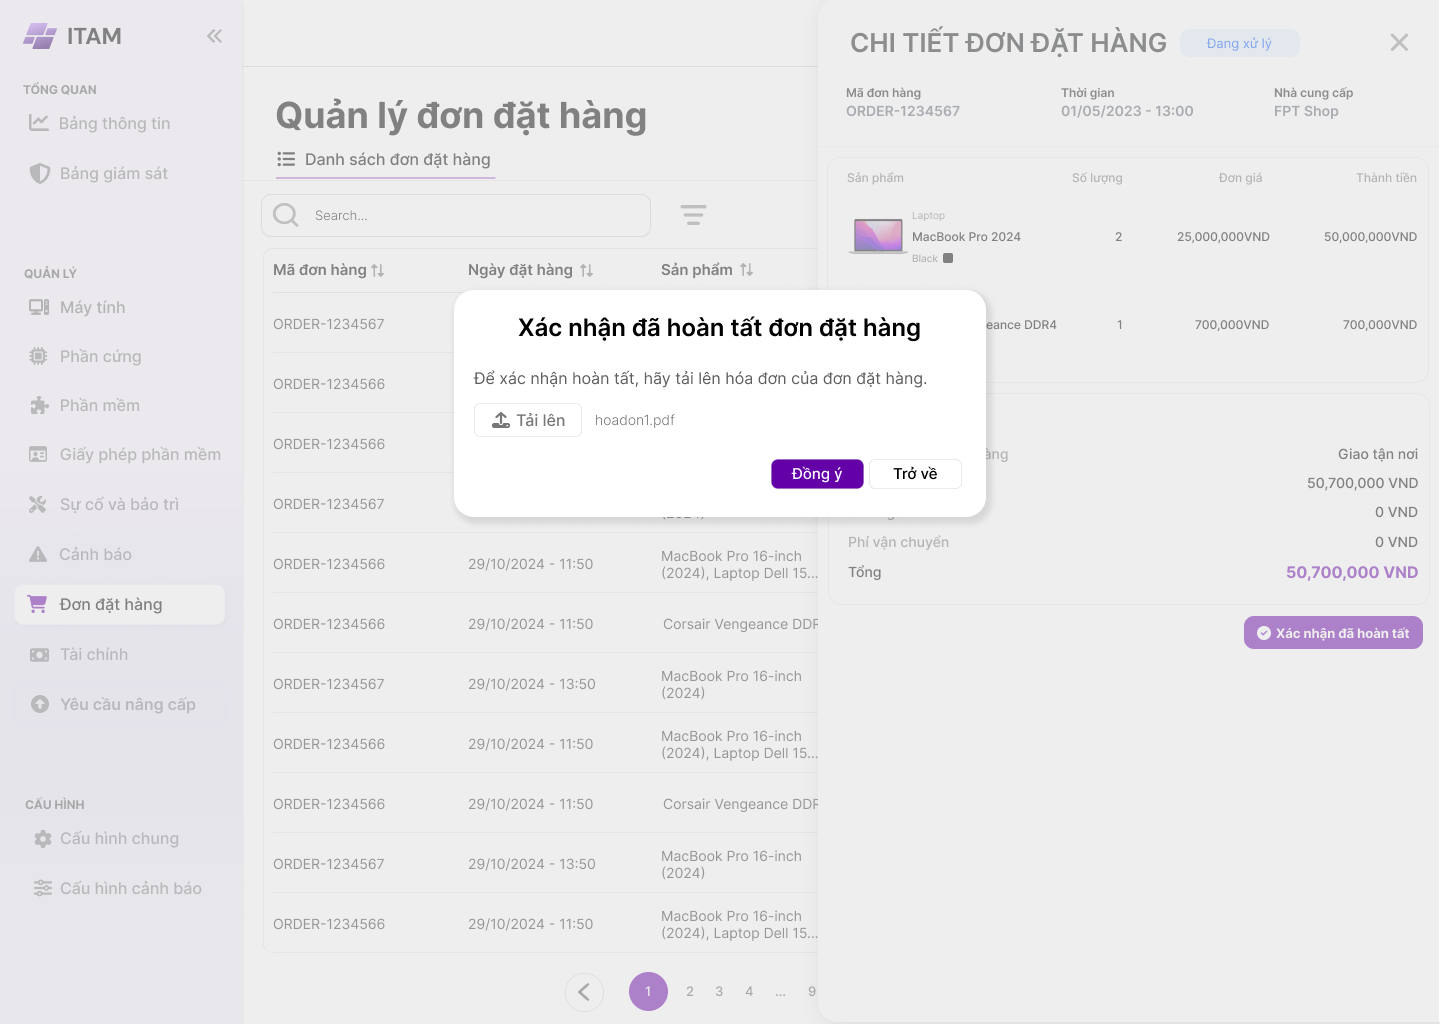
\includegraphics[width=14cm]{Images/C5/UI/Feature-Quản lý đơn đặt hàng 2.2.png}
%     \vspace{15pt}
%     \caption{Giao diện Quản lý đơn đặt hàng 3}
% \end{figure}
% \begin{figure}[H]
%     \centering
%     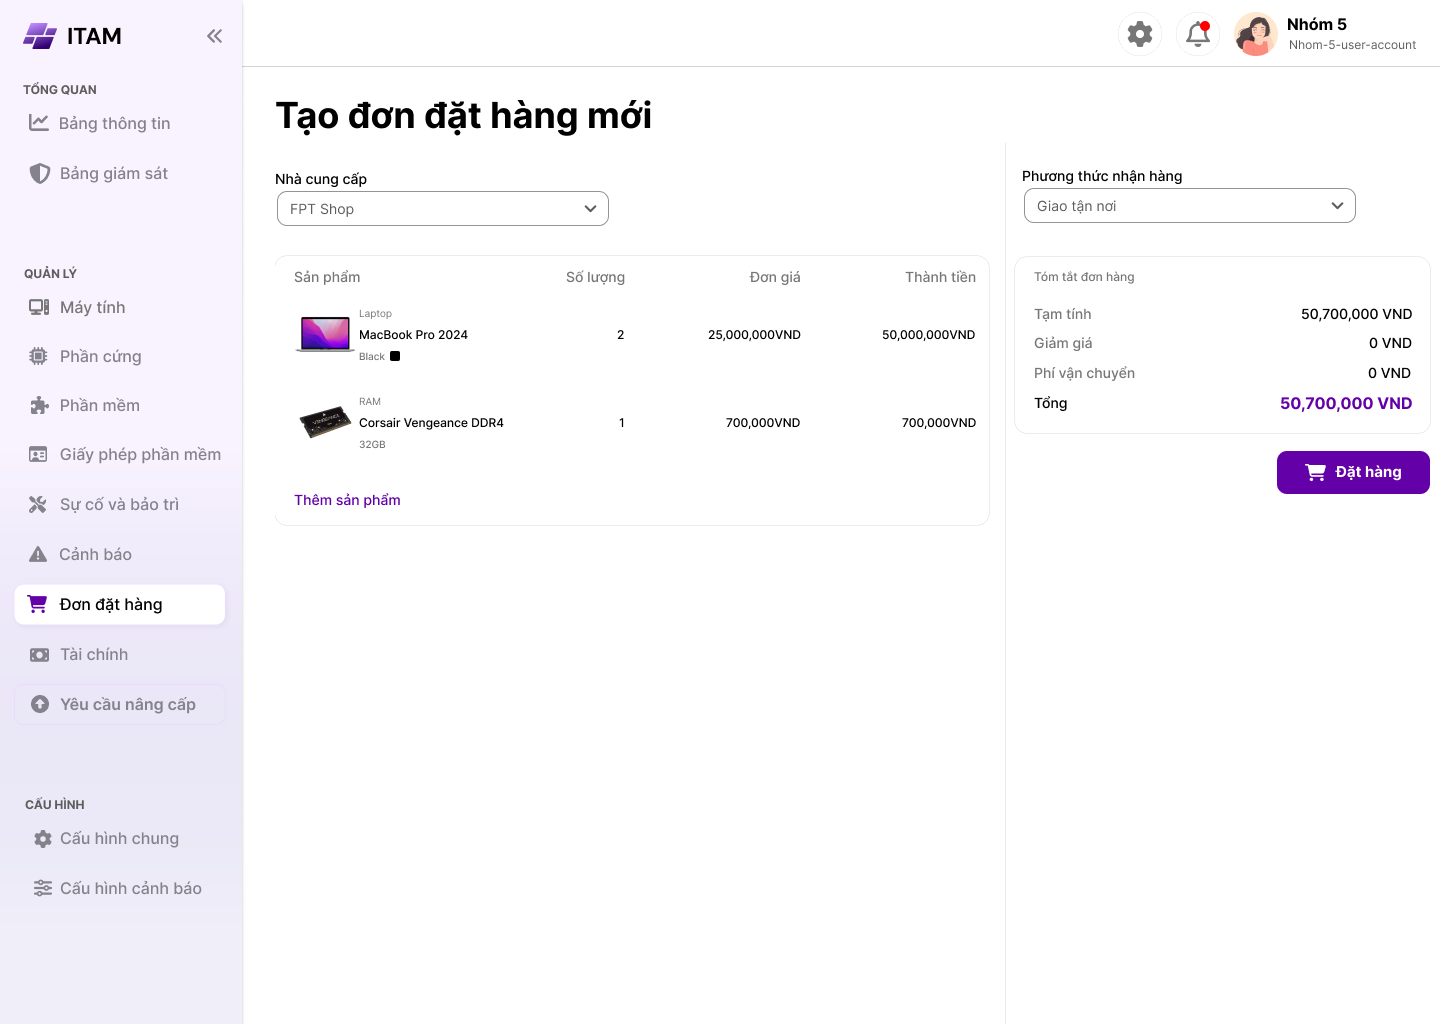
\includegraphics[width=14cm]{Images/C5/UI/Feature-Quản lý đơn đặt hàng 3.1.png}
%     \vspace{15pt}
%     \caption{Giao diện Quản lý đơn đặt hàng 3}
% \end{figure}
% \begin{figure}[H]
%     \centering
%     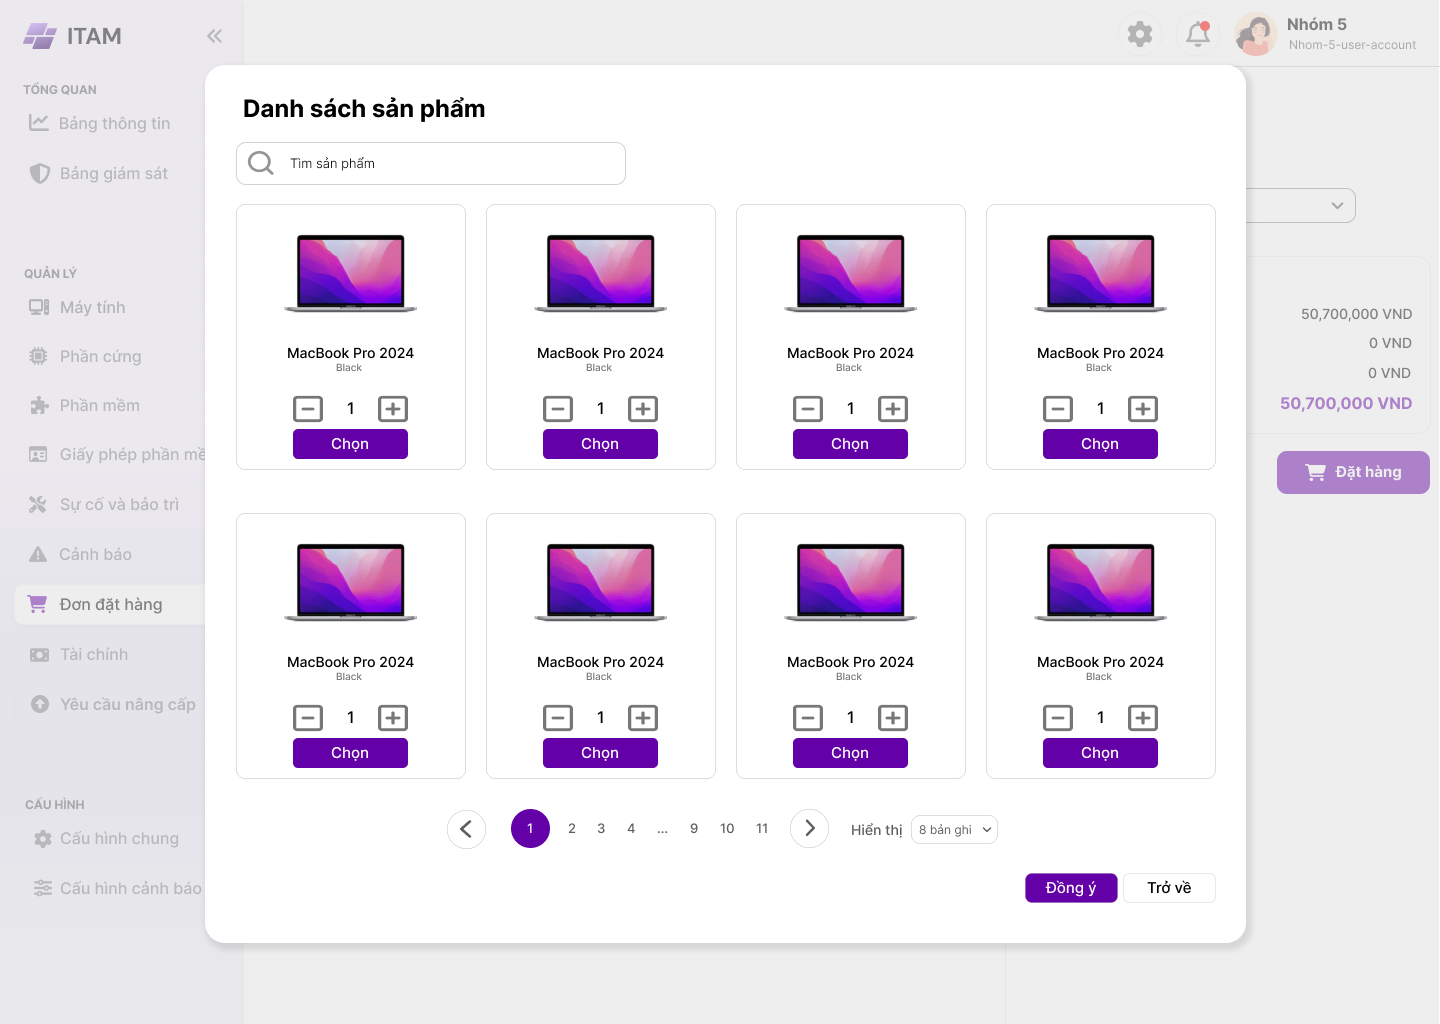
\includegraphics[width=14cm]{Images/C5/UI/Feature-Quản lý đơn đặt hàng 3.2.png}
%     \vspace{15pt}
%     \caption{Giao diện Quản lý đơn đặt hàng 5}
% \end{figure}
% \begin{figure}[H]
%     \centering
%     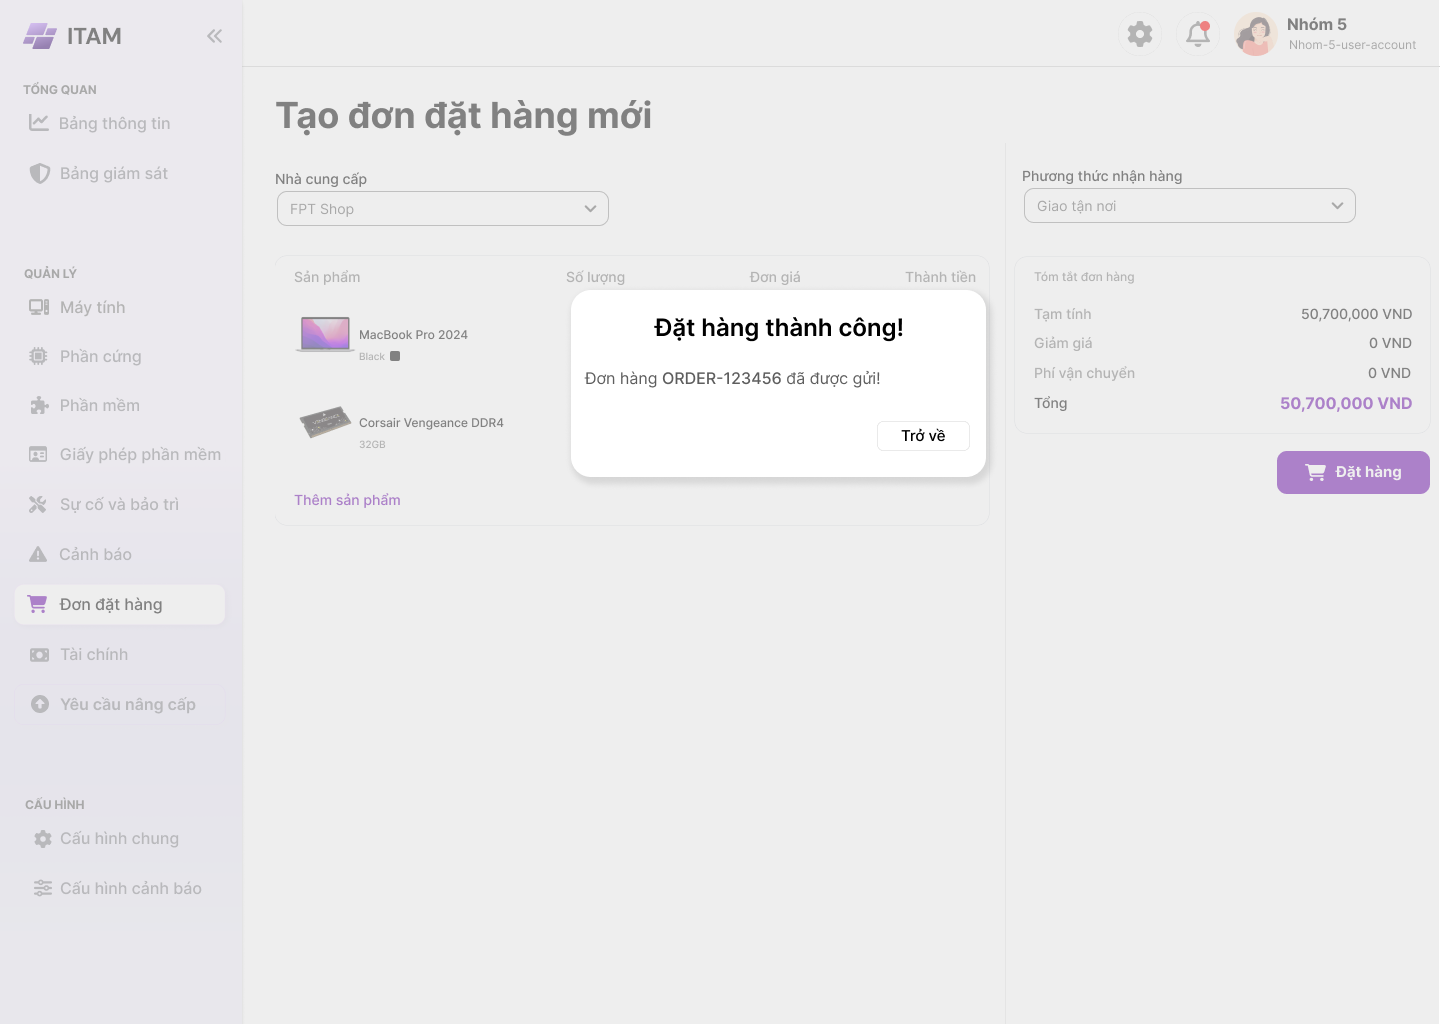
\includegraphics[width=14cm]{Images/C5/UI/Feature-Quản lý đơn đặt hàng 3.3.png}
%     \vspace{15pt}
%     \caption{Giao diện Quản lý đơn đặt hàng 6}
% \end{figure}

\item{Quản lý giấy phép phần mềm}\\
Quản lý giấy phép mềm hiển thị danh sách và thông tin của các giấy phép phần mềm có trong hệ thống (xem thêm chi tiết ở phụ lục).
% \begin{figure}[H]
%     \centering
%     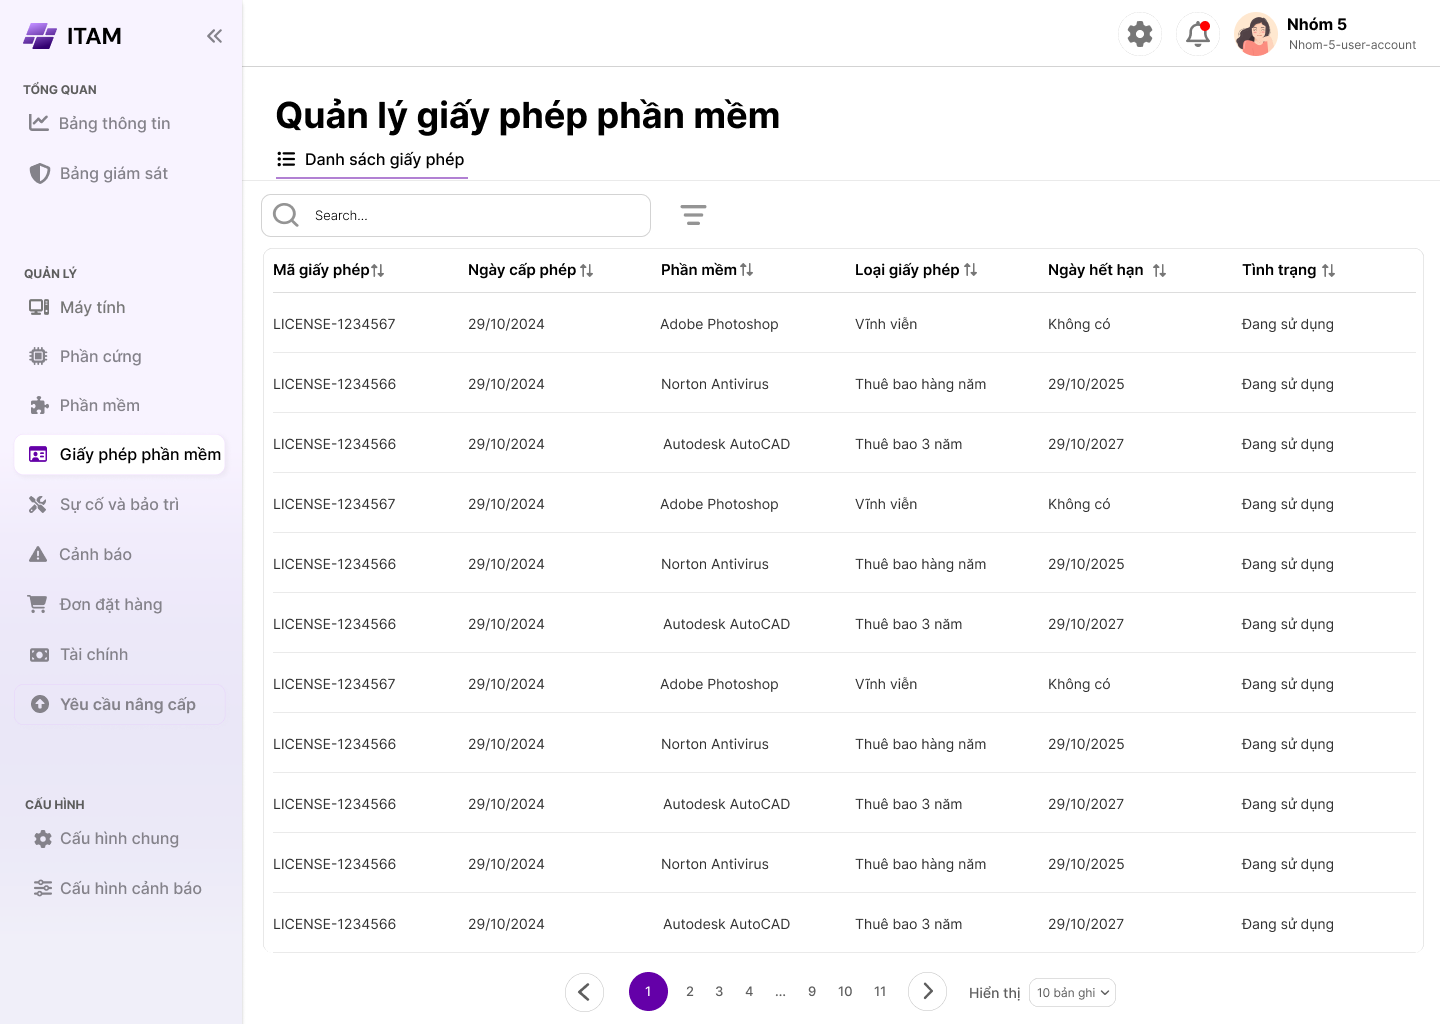
\includegraphics[width=14cm]{Images/C5/UI/Feature-Quản lý giấy phép phần mềm.png}
%     \vspace{15pt}
%     \caption{Giao diện Quản lý giấy phép phần mềm}
% \end{figure}

\item{Quản lý cấu hình cảnh báo}\\
Người dùng truy cập vào Cấu hình cảnh báo để điều chỉnh các ngưỡng của cảnh báo cho các máy tính trong hệ thống. Dựa vào các ngưỡng này, cảnh báo sẽ được sinh ra (xem thêm chi tiết ở phụ lục).
% \begin{figure}[H]
%     \centering
%     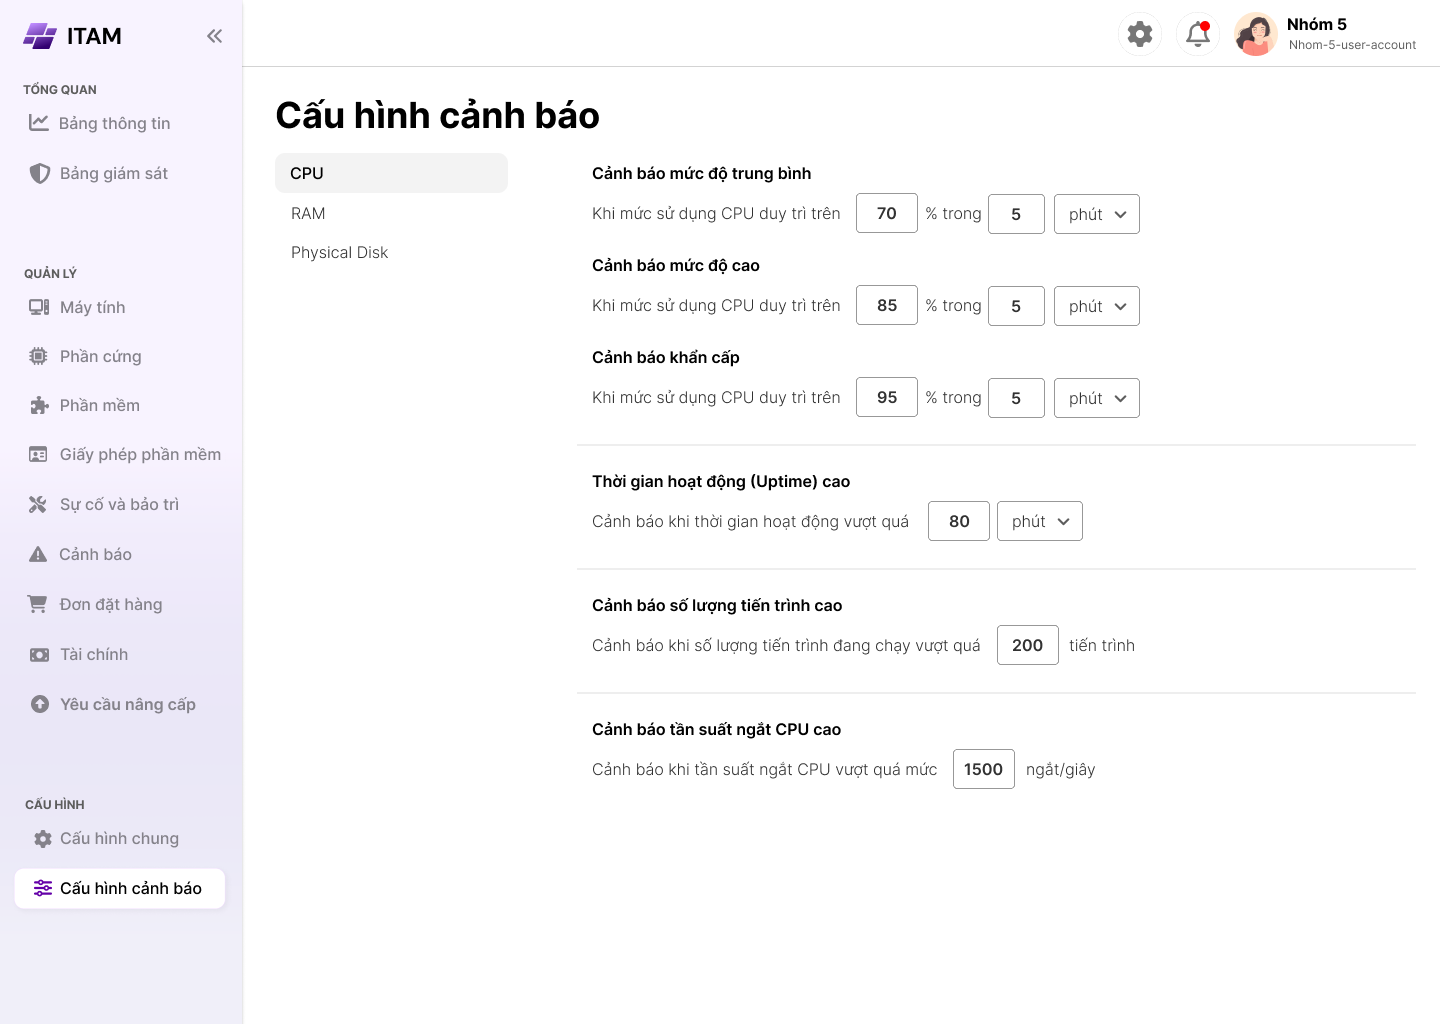
\includegraphics[width=14cm]{Images/C5/UI/Feature-Cấu hình cảnh báo 1.png}
%     \vspace{15pt}
%     \caption{Giao diện Quản lý cấu hình cảnh báo 1}
% \end{figure}
% \begin{figure}[H]
%     \centering
%     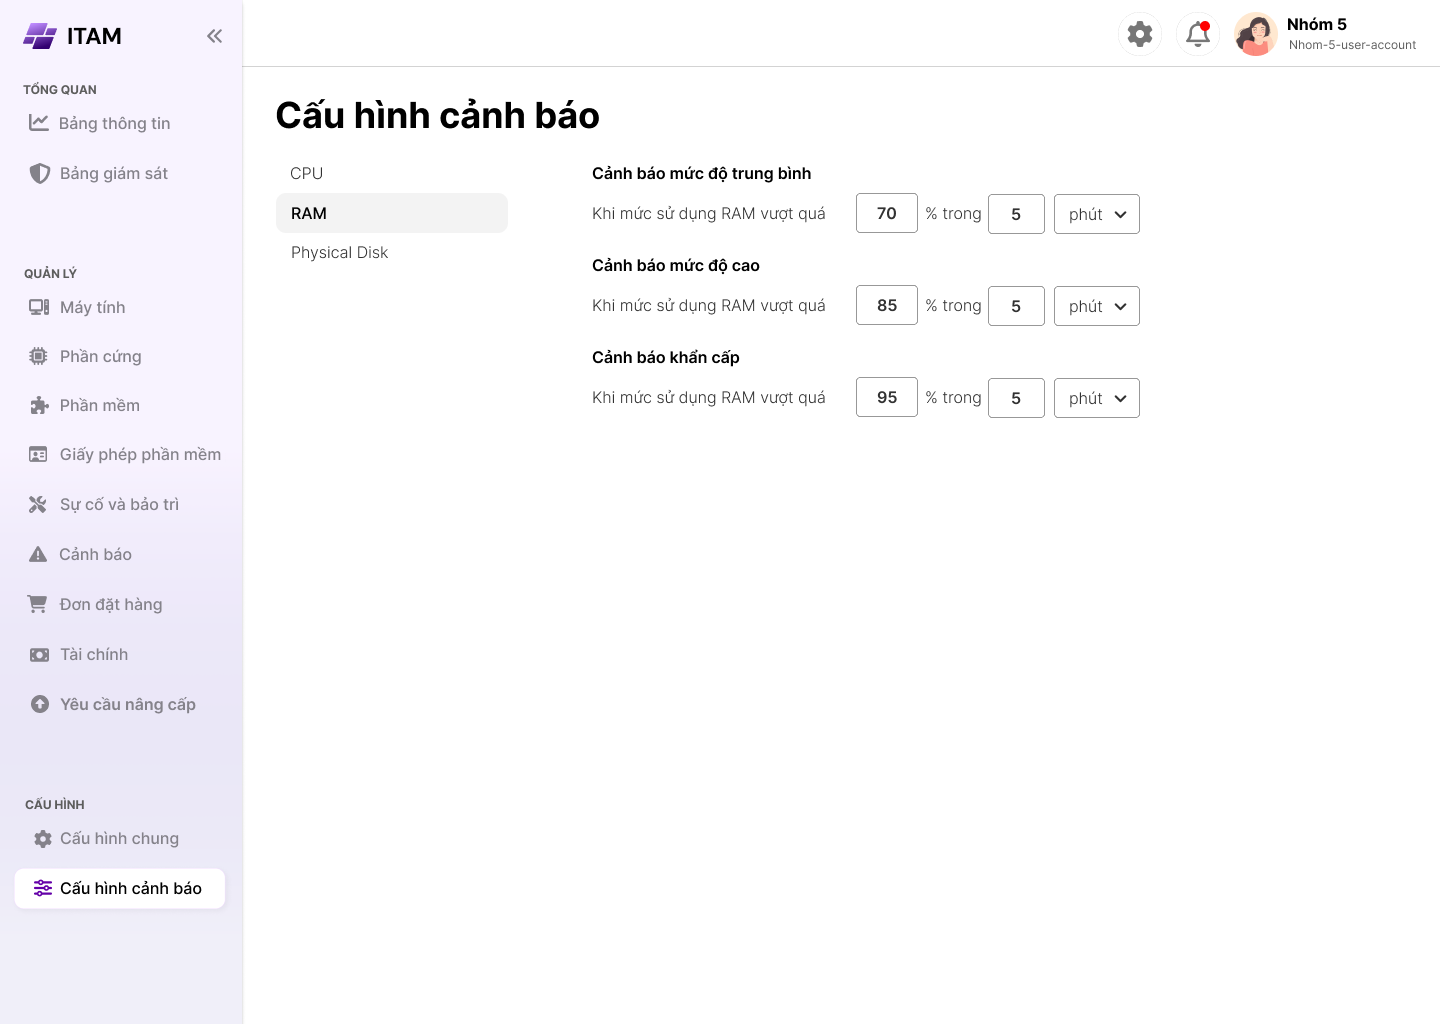
\includegraphics[width=14cm]{Images/C5/UI/Feature-Cấu hình cảnh báo 5.png}
%     \vspace{15pt}
%     \caption{Giao diện Quản lý cấu hình cảnh báo 2}
% \end{figure}
% \begin{figure}[H]
%     \centering
%     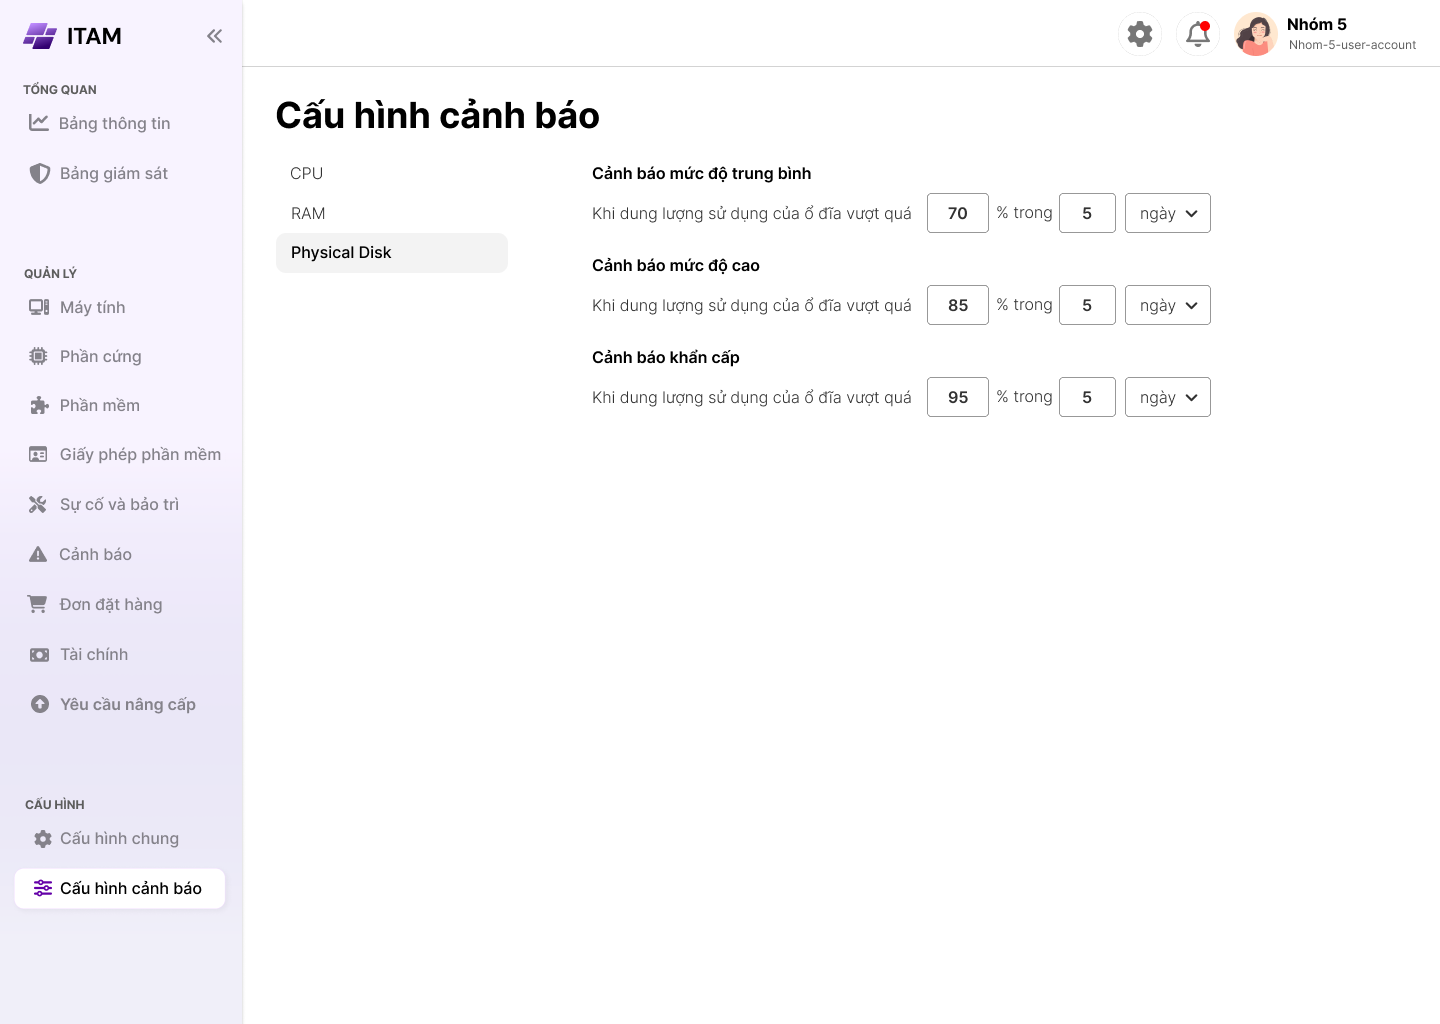
\includegraphics[width=14cm]{Images/C5/UI/Feature-Cấu hình cảnh báo 6.png}
%     \vspace{15pt}
%     \caption{Giao diện Quản lý cấu hình cảnh báo 3}
% \end{figure}

\end{itemize}
\subsection{Kết chương}
\noindent Trong quá trình phát triển một hệ thống hoàn chỉnh, phân tích và thiết kế đóng vai trò cốt lõi.
Chương này nhóm đã ba nội dung chính:
\begin{itemize}
    \item \textbf{Phân tích}: Mô hình hóa quy trình nghiệp vụ và các tương tác trong hệ thống.
    \item \textbf{Giải pháp công nghệ}: Đề xuất các giải pháp, đặc biệt là xử lý thời gian thực để đáp ứng yêu cầu nghiệp vụ.
    \item \textbf{Thiết kế}: Bao gồm thiết kế kiến trúc hệ thống, cơ sở dữ liệu, chi tiết bên trong và giao diện người dùng.
\end{itemize}
Qua phần phân tích nhóm đã đưa ra mô hình hóa nghiệp vụ cho các qui trình: giám sát tài sản, quản lý vòng đời tài sản, cảnh báo, quản lý đơn đặt hàng. Bên cạnh đó nhóm cũng đưa ra các use case cho hệ thống để trình bày các luồng thực thi cho hệ thống.\\ \\ 
Đến phần giải pháp công nghệ, nhóm đã trình bày các khái niệm, khía cạnh liên quan đến thu thập và xử lý dữ liệu thời gian thực. Ngoài ra nhóm cũng đã đi sâu vào phần công nghệ Kafka (công nghệ cốt lõi mà nhóm đã chọn) và so sánh Kafka với hai loại công nghệ khác là .\\ \\
Cuối cùng là phần thiết kế, trong phần này, nhóm đã đưa ra một kiến trúc hệ thống gồm 3 lớp là Presentation, Application, Storage. Từ đó nhóm đã lựa chọn các công nghệ cho Front-End là Angular và Back-end là ASP.NET Core, cơ sở dữ liệu là MSSQL. Nhóm cũng đã thiết kế ERD, làm rõ mối quan hệ giữa các đối tượng dữ liệu của hệ thống. Bên cạnh đó, nhóm cũng đã trình bày chi tiết bên trong qua class diagram và giao diện bên ngoài qua figma.






